% Options for packages loaded elsewhere
\PassOptionsToPackage{unicode}{hyperref}
\PassOptionsToPackage{hyphens}{url}
%
\documentclass[
  a4paper,
]{book}
\usepackage{amsmath,amssymb}
\usepackage{iftex}
\ifPDFTeX
  \usepackage[T1]{fontenc}
  \usepackage[utf8]{inputenc}
  \usepackage{textcomp} % provide euro and other symbols
\else % if luatex or xetex
  \usepackage{unicode-math} % this also loads fontspec
  \defaultfontfeatures{Scale=MatchLowercase}
  \defaultfontfeatures[\rmfamily]{Ligatures=TeX,Scale=1}
\fi
\usepackage{lmodern}
\ifPDFTeX\else
  % xetex/luatex font selection
\fi
% Use upquote if available, for straight quotes in verbatim environments
\IfFileExists{upquote.sty}{\usepackage{upquote}}{}
\IfFileExists{microtype.sty}{% use microtype if available
  \usepackage[]{microtype}
  \UseMicrotypeSet[protrusion]{basicmath} % disable protrusion for tt fonts
}{}
\makeatletter
\@ifundefined{KOMAClassName}{% if non-KOMA class
  \IfFileExists{parskip.sty}{%
    \usepackage{parskip}
  }{% else
    \setlength{\parindent}{0pt}
    \setlength{\parskip}{6pt plus 2pt minus 1pt}}
}{% if KOMA class
  \KOMAoptions{parskip=half}}
\makeatother
\usepackage{xcolor}
\usepackage{longtable,booktabs,array}
\usepackage{calc} % for calculating minipage widths
% Correct order of tables after \paragraph or \subparagraph
\usepackage{etoolbox}
\makeatletter
\patchcmd\longtable{\par}{\if@noskipsec\mbox{}\fi\par}{}{}
\makeatother
% Allow footnotes in longtable head/foot
\IfFileExists{footnotehyper.sty}{\usepackage{footnotehyper}}{\usepackage{footnote}}
\makesavenoteenv{longtable}
\usepackage{graphicx}
\makeatletter
\def\maxwidth{\ifdim\Gin@nat@width>\linewidth\linewidth\else\Gin@nat@width\fi}
\def\maxheight{\ifdim\Gin@nat@height>\textheight\textheight\else\Gin@nat@height\fi}
\makeatother
% Scale images if necessary, so that they will not overflow the page
% margins by default, and it is still possible to overwrite the defaults
% using explicit options in \includegraphics[width, height, ...]{}
\setkeys{Gin}{width=\maxwidth,height=\maxheight,keepaspectratio}
% Set default figure placement to htbp
\makeatletter
\def\fps@figure{htbp}
\makeatother
\setlength{\emergencystretch}{3em} % prevent overfull lines
\providecommand{\tightlist}{%
  \setlength{\itemsep}{0pt}\setlength{\parskip}{0pt}}
\setcounter{secnumdepth}{5}
\ifLuaTeX
\usepackage[bidi=basic]{babel}
\else
\usepackage[bidi=default]{babel}
\fi
\babelprovide[main,import]{ngerman}
% get rid of language-specific shorthands (see #6817):
\let\LanguageShortHands\languageshorthands
\def\languageshorthands#1{}
\usepackage[utf8]{inputenc}
\usepackage{booktabs}
\usepackage{amsthm}
\usepackage{tcolorbox}
\usepackage{hyphenat}
\usepackage[top=20mm,bottom=20mm,left=20mm,right=20mm]{geometry}

\makeatletter
\def\thm@space@setup{%
  \thm@preskip=8pt plus 2pt minus 4pt
  \thm@postskip=\thm@preskip
}
\makeatother

\hyphenation{Me-dien-pä-da-gog-ik Bild-ungs-in-for-ma-tik Kom-mu-ni-ka-ti-ons-me-di-en Hand-lungs-mus-tern So-zia-li-sa-ti-ons Ein-satz-mög-lich-kei-ten Rah-men-be-din-gun-gen Un-ter-su-chungs-zu-sam-men-hang Ver-gleichs-di-men-sio-nen Trans-for-ma-ti-ons-dy-na-mi-ken Hand-lungs-se-quen-zen De-si-gn-wis-sen-schaf-ten Vor-aus-set-zun-gen au-to-ope-ra-tio-na-le Ge-gen-stands-be-rei-che Lern-ma-nage-ment-sys-te-me Soft-ware-schnitt-stel-len Aus-ga-be-mög-lich-kei-ten An-wen-der-in-nen Be-nut-zungs-schnitt-stel-len Pro-duk-ti-ons-be-din-gun-gen kul-tur-wis-sen-schaft-lich er-zie-hungs-wis-sen-schaft-li-chen Kom-pe-tenz-pro-fi-le Trans-for-ma-ti-ons-pro-zess Po-si-ti-ons-be-stim-mun-gen Ge-stal-tungs-pro-zes-ses Hand-lungs-mög-lich-kei-ten Me-tho-den-aus-bil-dung}

% Manuelle Titel-Anpassungen
\renewcommand{\contentsname}{Inhaltsverzeichnis}
\addto\captionsenglish{\renewcommand{\chaptername}{Kapitel}}

%Formatierung der Diskussionskästen
\newtcolorbox{blackbox}{
  colback=red,
  colframe=red,
  coltext=white,
  boxsep=5pt,
  arc=4pt}

%Formatierung der Whitebox
\newtcolorbox{whitebox}{
  colback=white,
  colframe=black,
  coltext=black,
  boxsep=5pt,
  arc=0pt}

%Formatierung der Lizenzkästen
\newenvironment{licencebox}[1]
  {
  \begin{itemize}
  \renewcommand{\labelitemi}{
    \raisebox{-.7\height}[0pt][0pt]{
      {\setkeys{Gin}{width=6em,keepaspectratio}
        
\includegraphics{figures/by-sa.png}}
    }
  }
  \setlength{\fboxsep}{1 em}
  \begin{whitebox}
  \item
  }
  {
  \end{whitebox}
  \end{itemize}
  }

\AtBeginDocument{\let\maketitle\relax}

\usepackage{fancyhdr}
\pagestyle{fancy}
\fancyhf{} % Alle Kopf- und Fußzeilen bereinigen
\fancyhead[LE,RO]{\rightmark} % Nur Unterkapitel (Abschnittstitel) in Kopfzeile anzeigen
\fancyfoot[C]{\thepage}


\raggedbottom

\let\cleardoublepage\clearpage



\ifLuaTeX
  \usepackage{selnolig}  % disable illegal ligatures
\fi
\usepackage[]{natbib}
\bibliographystyle{apa-good-german}
\usepackage{bookmark}
\IfFileExists{xurl.sty}{\usepackage{xurl}}{} % add URL line breaks if available
\urlstyle{same}
\hypersetup{
  pdftitle={Digitale Medienbildung},
  pdfauthor={Christoph Richter},
  pdflang={de},
  hidelinks,
  pdfcreator={LaTeX via pandoc}}

\title{Digitale Medienbildung}
\usepackage{etoolbox}
\makeatletter
\providecommand{\subtitle}[1]{% add subtitle to \maketitle
  \apptocmd{\@title}{\par {\large #1 \par}}{}{}
}
\makeatother
\subtitle{Ein Denk- und Werkzeugkasten}
\author{Christoph Richter}
\date{2024: zuletzt kompiliert 2024-11-01}

\begin{document}
\maketitle

\pagenumbering{gobble}

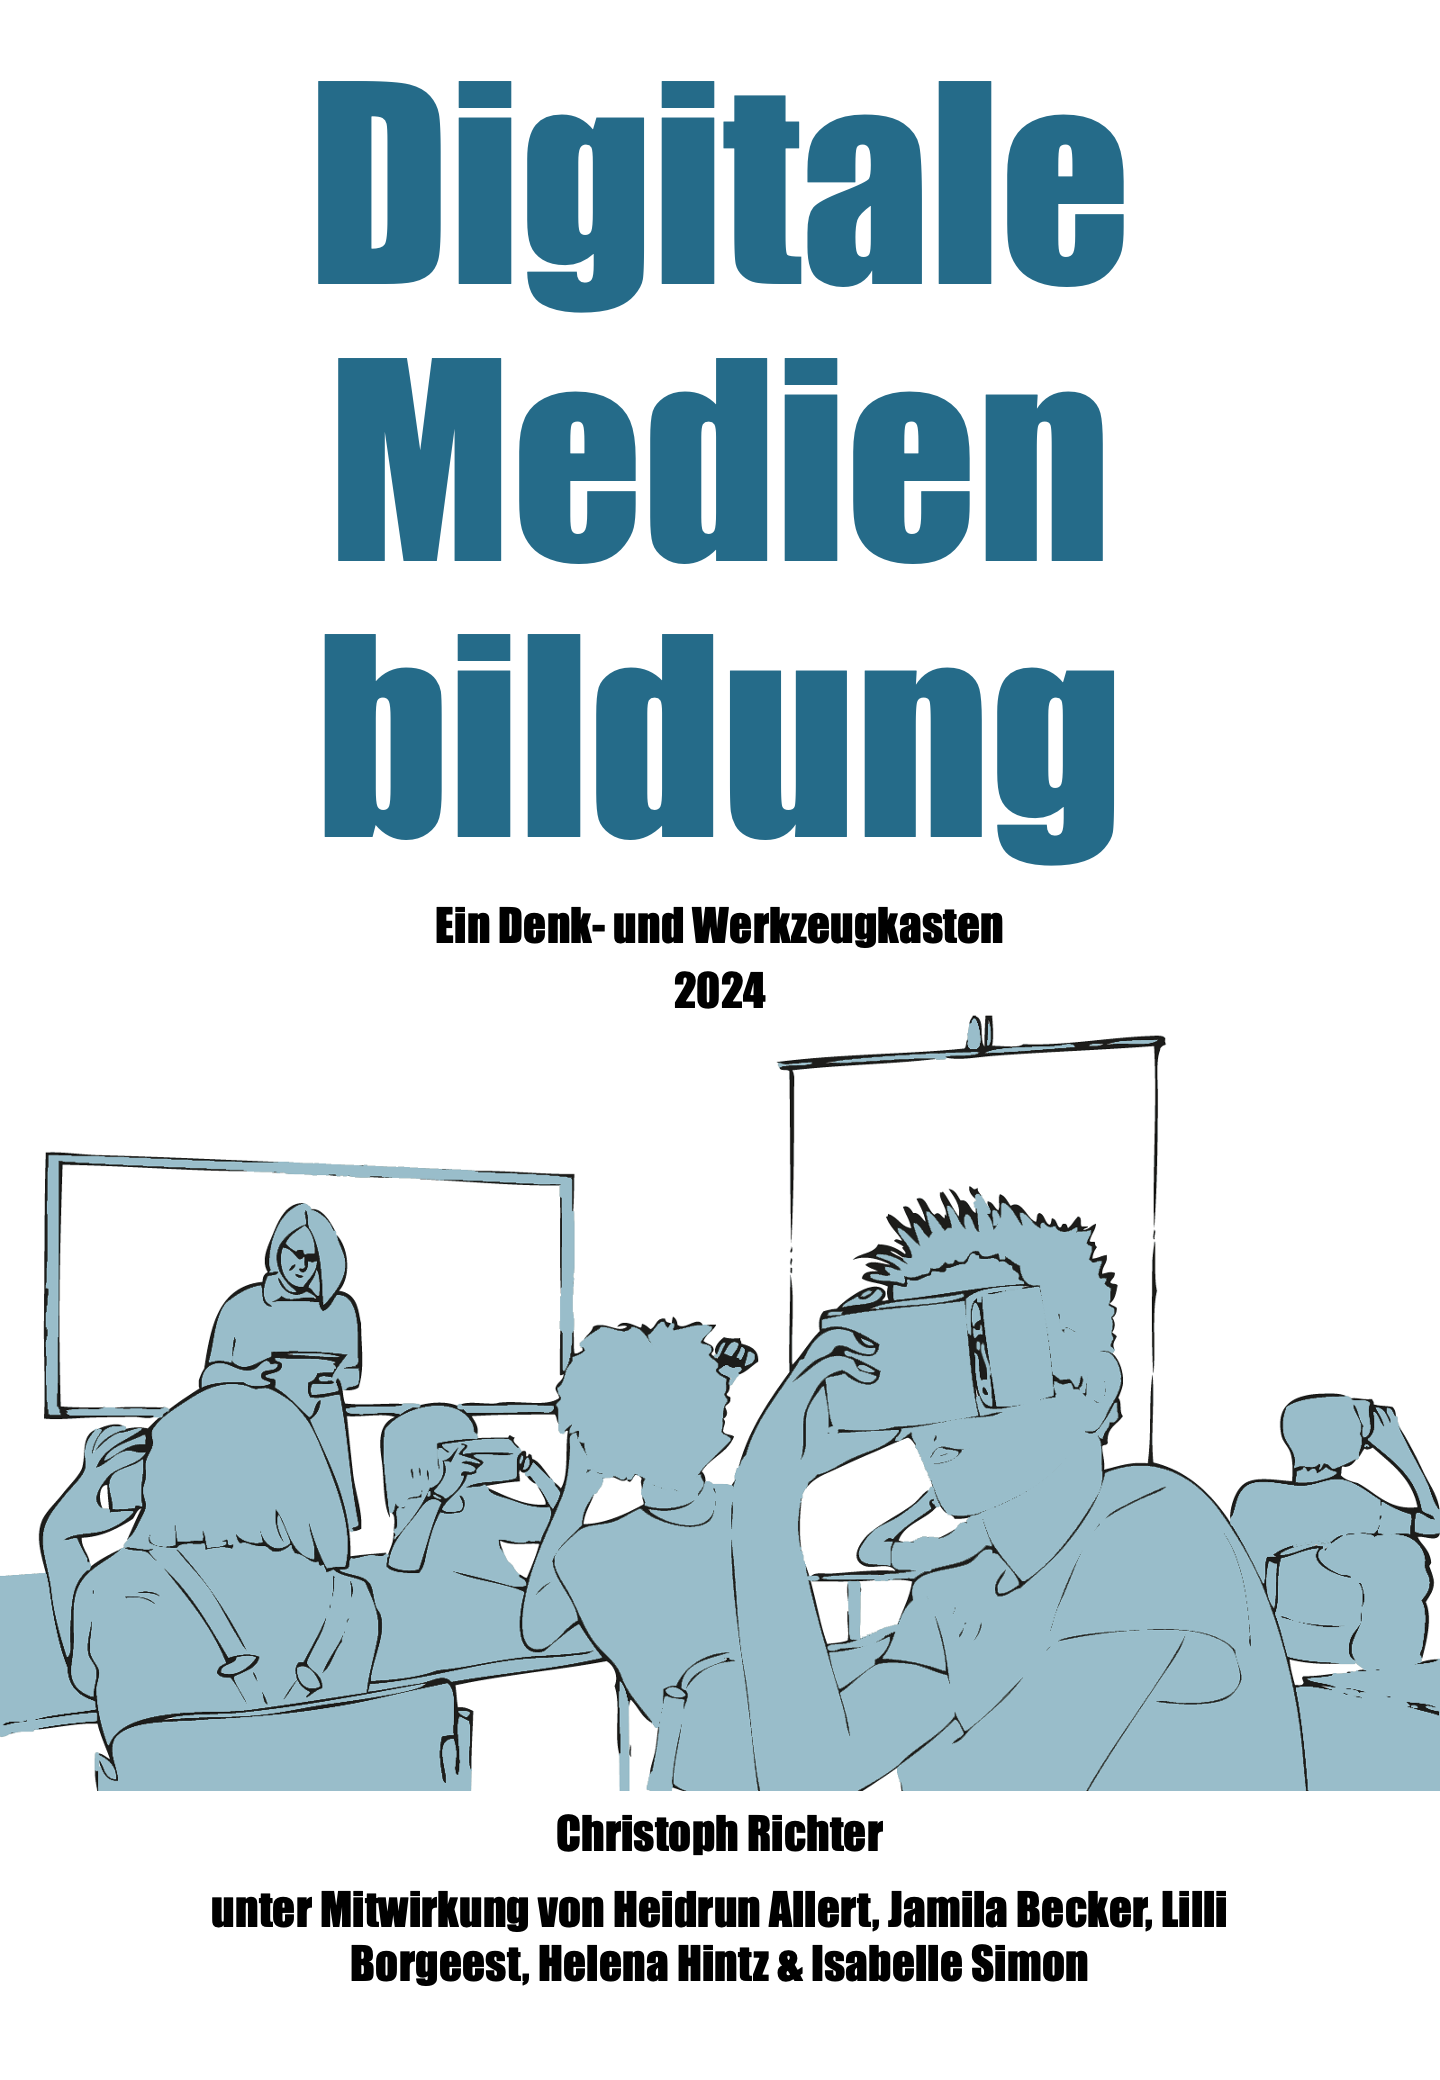
\includegraphics[width=\textwidth, height=0.99\textheight]{Figures/Cover.png}


\newpage
~\vfill
\thispagestyle{empty}

\noindent IMPRESSUM\\
\noindent »Digitale Medienbildung - Ein Denk- und Werkzeugkasten«\\
\noindent Christoph Richter\\
\noindent unter Mitwirkung von Heidrun Allert, Jamila Becker, Lilli Borgeest, Helena Hintz und Isabelle Simon\\
\\
\noindent 2024\\
\\
\noindent Herausgeberin:\\
Heidrun Allert\\
Olshausenstr. 75\\
24118 Kiel\\
Deutschland\\
allert(at)paedagogik.uni-kiel.de\\
\\
\noindent Web: \href{https://christoph-mp.github.io/Digitale-Medienbildung/}{christoph-mp.github.io/Digitale-Medienbildung}\\ % URL

\noindent DOI: \href{https://zenodo.org/records/13778113}{10.5281/zenodo.13778113}\\ % DOI


\includegraphics[width=0.15\textwidth]{"Figures/by-sa.png"}\par\vspace{1cm}


\noindent Dieses Werk ist unter der Creative-Commons-Lizenz Namensnennung – Weitergabe unter gleichen Bedingungen 4.0 International \href{https://creativecommons.org/licenses/by-sa/4.0/}{CC BY-SA 4.0} Lizenz veröffentlicht. Den vollständigen Lizenztext finden Sie unter \href{https://creativecommons.org/licenses/by-sa/4.0/deed.de}{https://creativecommons.org/licenses/by-sa/4.0/deed.de}.\\ % License information


\newpage
\pagenumbering{arabic}

{
\setcounter{tocdepth}{1}
\tableofcontents
}
\chapter*{Vorwort}\label{vorwort}
\addcontentsline{toc}{chapter}{Vorwort}

Der vorliegende ›Denk- und Werkzeugkasten‹ zum Themenfeld der Digitalen Medienbildung richtet sich an Lehramtstudierende und Lehrer*innen, aber auch an Medienpädagog*innen und andere Personen, die sich in schulischen und außerschulischen Handlungsfeldern mit Fragen der Digitalisierung befassen und sich damit auseinandersetzen, in welcher Weise digitale Technologien unsere sozialen, gesellschaftlichen und kulturellen Praktiken transformieren.

Als Denk- und Werkzeugkasten beinhaltet dieses Dokument verschiedene theoretische und methodische Ansatzpunkte zur eigenständigen wie auch gemeinsamen Erkundung digitaler Transformationsprozesse. Jedes der 14 Kapitel nähert sich dem Themenfeld der Digitalen Medienbildung aus einer spezifischen Perspektive. Nähere Informationen zum Aufbau und den didaktischen Leitgedanken finden sich in den Abschnitten \hyperref[keine-gebrauchsanweisung]{1.3} sowie \hyperref[inhalte-der-materialsammlung]{1.4}.

Das Dokument steht als freie und offene Ressource zur Verfügung. Weitere Informationen zum Kopieren, Ändern oder Mitwirken am Denk- und Werkzeugkasten finden Sie weiter unten.

\section{Entstehungszusammenhang und Danksagung}\label{entstehungszusammenhang-und-danksagung}

Der Denk- und Werkzeugkasten ist in der Abteilung für Medienpädagogik/Bildungsinformatik der Christian-Albrechts-Universität zu Kiel im Rahmen des Projekts \href{https://www.medienpaedagogik.uni-kiel.de/de/profil/entwicklungslinien-digitaler-kultur-digitale-kulturtechniken-und-wissenspraktiken}{»Entwicklungslinien digitaler Kultur, digitale Kulturtechniken und Wissenspraktiken«} unter Leitung von Frau Prof.~Dr.~Heidrun Allert entstanden. Das Projekt wurde aus Mitteln des Strategie- und Exzellenzbudgets des Ministeriums für Bildung, Wissenschaft und Kultur (MBWK) in Schleswig-Holstein im Zeitraum von 2021 bis 2024 gefördert.

Die Erstellung dieses Dokuments wäre ohne den engen Austausch mit der Projektleitung wie auch den am Projekt beteiligten wissenschaftlichen Hilfkräften nicht möglich gewesen. Sowohl Jamila Becker, Lilli Borgeest, Helena Hintz und Isabelle Simon haben die Entwicklung der Texte nicht nur formal, sondern auch inhaltlich eng begleitet und durch ihr Feedback wesentlich zu deren Qualität beigetragen. Jamila Becker, Helena Hintz und Isabelle Simon haben zudem nicht nur Beispiele (siehe Anhang), sondern auch einzelne Impulse und Leittexte beigesteuert und Lilli Borgeest hat einen wesentlichen Beitrag zur digitalen Umsetzung geleistet. Darüber hinaus möchte ich mich bei Heidrun Allert für den engen und kontinuierlichen Austausch zu inhaltlichen wie auch didaktischen Fragen bedanken, die dem Dokument letztlich seine Struktur und Form gegeben haben.

Schließlich gilt mein Dank auch den Studierenden, die sich während der Projektlaufzeit in einer Reihe von Lehrveranstaltungen mit den Inhalten und Ansätzen des Denk- und Werkzeugkastens auseinandergesetzt und hilfreiche Rückmeldungen zu dessen Weiterentwicklung gegeben haben.

\section{Lizenz \& Autor*innenschaft}\label{lizenz-autorinnenschaft}

~

Das gesamte Werk ist unter einer Creative Commons \href{https://creativecommons.org/licenses/by-sa/4.0/}{CC BY-SA 4.0} Lizenz veröffentlicht. Diese Lizenz erlaubt unter der Voraussetzung der Namensnennung der Urheber*innen und der Angabe der Lizenzbedingungen die Bearbeitung, Vervielfältigung und Verbreitung des Materials in jedem Format oder Medium für beliebige Zwecke, auch kommerzieller Art. Bei einer Bearbeitung oder Veränderung der Originalfassung dieses Werks müssen alle neuen Version unter derselben Lizenz \href{https://creativecommons.org/licenses/by-sa/4.0/}{CC BY-SA 4.0} veröffentlicht werden.

Ausführlichere Informationen zu den Lizenzbedingungen finden Sie unter: \url{https://creativecommons.org/licenses/by-sa/4.0/deed.de}.

~

\textbf{Angaben zur Autor*innenschaft}

Soweit nicht anders angegeben, wurden die Inhalte des Denk- und Werkzeugkastens von \href{Mailto:richter@paedagogik.uni-kiel.de}{Christoph Richter} erstellt.

Das Kapitel 1 \hyperref[digitale-medienbildung]{›Digitale Medienbildung‹} wurde von Christoph Richter und Heidrun Allert verfasst.

Der Impuls \hyperref[mein-lernkosmos]{›Mein Lernkosmos‹} sowie das Beispiel \hyperref[beispiel-blinkist]{›Blinkist‹} wurde von Helena Hintz verfasst.

Das Beispiel \hyperref[beispiel-whatsapp]{›WhatsApp‹} wurde von Jamila Becker erstellt.

Der Leittext \hyperref[partizipationsorientierter-technikeinsatz]{›Partizipationsorientierter Technikeinsatz‹} wurde von Isabelle Simon und Christoph Richter erstellt.

Soweit nicht anders angegeben, wurden alle Grafiken und Abbildungen von den jeweiligen Autor*innen selbst erstellt und unterliegen derselben Lizenz wie das gesamte Dokument.

\section{Kopieren des Denk- und Werkzeugkastens}\label{kopieren-des-denk--und-werkzeugkastens}

Dieses Dokument wurde in R-Studio unter Verwendung von R Markdown geschrieben und mit dem Bookdown-Paket in ein Webbuchformat übersetzt.

Der gesamte Quellcode für die Kompilierung des Buches ist im GitHub-Repository für dieses Buch verfügbar: \url{https://github.com/Christoph-MP/Digitale-Medienbildung/}.

Sie können dieses Repository sowohl herunterladen als auch {[}forken{]}. Laden Sie anschließend die Rproj-Datei in R-Studio und kompilieren Sie dann das gesamte Buch. Anschließend können Sie die einzelnen .rmd-Dateien für jedes Kapitel inhaltlich und stilistisch ihren eigenen Bedürfnissen anpassen. Nähere Informationen zur Arbeit mit Bookdown finden Sie unter anderem in \href{https://www.crumplab.com/OER_bookdown/}{»Open tools for writing open interactive textbooks (and more).«} von M.J.C. Crump.

Wenn sie zu diesem Denk- und Werkzeugkasten beitragen möchten, können Sie Pull-Requests auf GitHub stellen oder Probleme und Anfragen auf der Registerkarte Probleme diskutieren.

\chapter{Digitale Medienbildung}\label{digitale-medienbildung}

\emph{(Autor*innen: Christoph Richter \& Heidrun Allert, 2022)}

Digitale Technologien sind zu einem integralen \textbf{Bestandteil unseres Alltags} geworden. Egal ob wir im Internet nach einem Kochrezept suchen, uns mit Hilfe unseres Smartphones zu einer Sehenswürdigkeit oder zum nächsten Bahnhof navigieren lassen, unseren Freund*innen eine Kurznachricht zukommen lassen oder mit unseren Kolleg*innen in der ›Cloud‹ arbeiten, überall haben wir es mit digitalen Technologien zu tun. Und auch dort, wo wir nicht direkt mit ihnen interagieren, mischen sie sich ein. Etwa indem sie Verkehrs-, Energie- und Warenflüsse steuern, Wetter- und Klimaprognosen erstellen, Fachwissen synthetisieren, Texte produzieren, zur Entwicklung neuer Medikamente oder auch von Waffentechnik verwendet werden.

In dem Maße, in dem uns digitale Technologien nicht mehr nur als ›bloße‹ Werkzeuge und Kommunikationsmedien dienen, sondern in immer umfassenderer Weise unsere individuellen Handlungs- und Erfahrungsspielräume prägen, werfen sie sowohl grundlegende bildungstheoretische wie auch bildungspraktische Fragen auf. Im Folgenden geht es um eine erste Annäherung an die \textbf{Begriffe der Digitalisierung und Digitalität} und die hieran anknüpfende Idee einer \textbf{›digitalen Medienbildung‹}.

\begin{figure}

{\centering 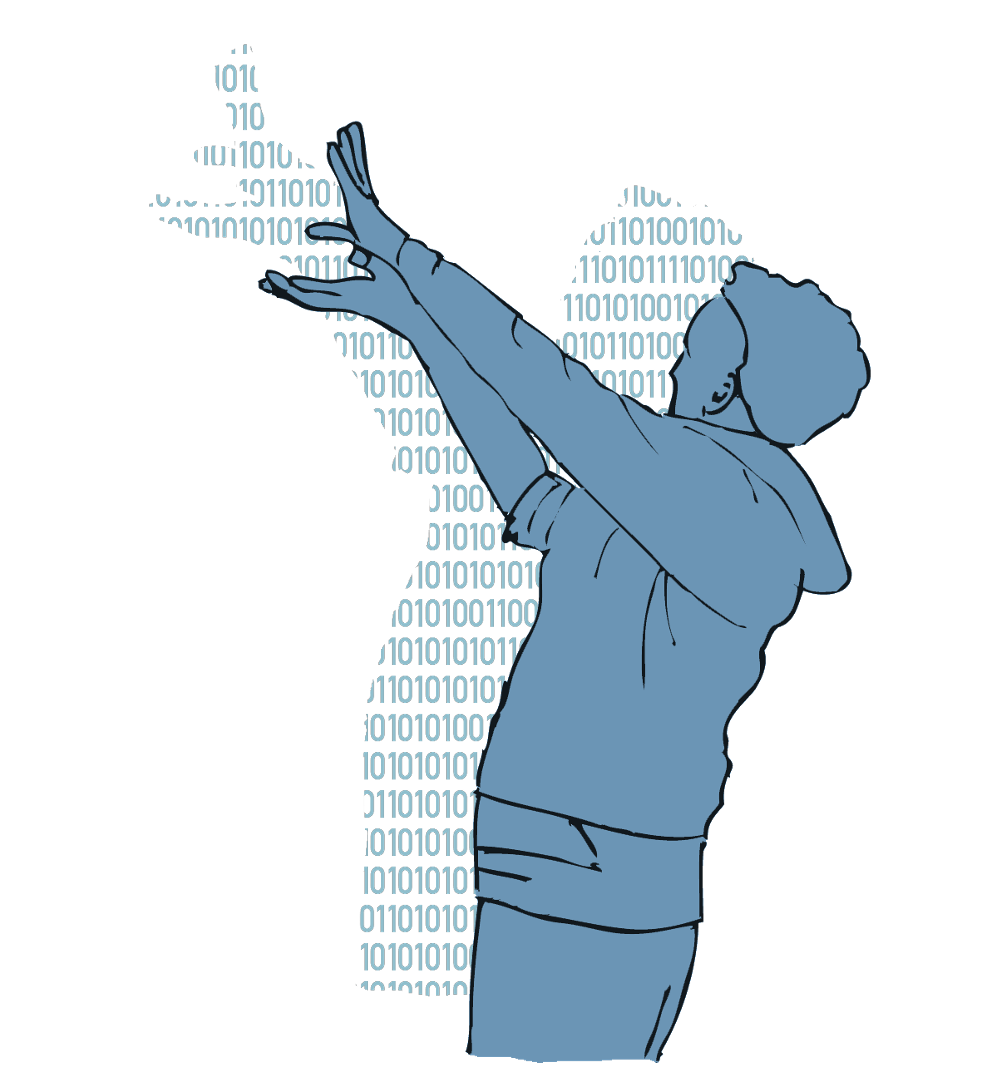
\includegraphics{Figures/01-1-Schattenspieler} 

}

\caption{Schattenspieler.}\label{fig:fig1}
\end{figure}

\section{Digitalisierung und Digitalität}\label{digitalisierung-und-digitalituxe4t}

Trotz seiner weiten Verbreitung ist der Begriff der ›Digitalisierung‹ mit verschiedenen Assoziationen behaftet. So verweist Digitalisierung in einem sehr engen Sinn auf die Überführung analoger Daten in ein von Computern verarbeitbares Format, wie etwa beim Scannen eines Textes oder der digitalen Aufzeichnung eines Musikstückes. Unter Digitalisierung wird aber auch die Delegation von Aufgaben und Entscheidungsprozessen an Computer verstanden, wie etwa bei der Verwendung eines Bankterminals zur Abwicklung von Überweisungen oder auch der Orientierung mittels eines digitalen Navigationsgeräts. Schließlich wird mit dem Begriff der Digitalisierung auf die tiefgreifende Veränderung sozialer, politischer und gesellschaftlicher Gefüge hingewiesen, etwa wenn sich durch den Einsatz von Informations- und Kommunikationstechnologien Arbeits- und Lebensbedingungen, Partizipationsmöglichkeiten oder Machverhältnisse transformieren \citep{brindaFrankfurtDreieckZurBildung2019}.

Für die aktuelle (medien-)pädagogische Diskussion ist insbesondere dieses letzte, sehr weit gefasste Begriffsverständnis von Interesse, da es Digitalisierung als einen kulturellen Transformationsprozess auffasst, der aufs engste mit unseren gemeinsamen Lebens- und Handlungsweisen wie auch unseren individuellen und kollektiven Selbstverständnissen verknüpft ist. Digitale Technologien sind aus dieser Perspektive nicht bloße Werkzeuge oder Instrumente, die wir zielgerichtet nutzen, sondern Kulturtechniken, die durch soziale Prozesse entstehen und zugleich unser soziales Miteinander nachhaltig prägen. So hat etwa die Entwicklung internetbasierter Suchmaschinen nicht nur unseren Zugang zu Informationen erweitert, sondern auch unsere Art des Suchens und den Umgang mit Informationen transformiert, während Social Media Plattformen es nicht nur möglich machen mit unseren Freunden, Bekannten und Verwandten in Kontakt zu bleiben, sondern auch neue Erwartungen und Interaktionsformen mit sich gebracht haben. Digitalisierung impliziert entsprechend immer auch die Veränderung unserer Lebenswelt, in dem sie »tief in die ökonomischen, aber auch in die politischen und kulturellen Verhältnisse ein{[}greift{]}« \citep[S. 33]{coyKulturenNichtBetreten2008}.

Um der sozialen und kulturellen Tragweite dieser Veränderungen Rechnung zu tragen und deutlich zu machen, dass der Prozess der Digitalisierung »so weit abgeschlossen ist, dass das Digitale eine omnipräsente, ubiquitäre Infrastruktur darstellt« \citep[S. 69]{jorissenSubjektivationUndAsthetische2018}, wird auch in der medienpädagogischen Diskussion vermehrt auf das Konzept der ›Digitalität‹ Bezug genommen. Im Unterschied zum Begriff der Digitalisierung, der eng mit technologischen Entwicklungen assoziiert ist, bezieht sich der Begriff der Digitalität auf einen »dominante{[}n{]} kulturelle{[}n{]} Raum, in dem wir uns bewegen, bzw. die dominante Bedingung, unter der wir uns bewegen« \citep[S. 4]{stalderWasIstDigitalitaet2021}. Das Konzept der Digitalität betont den Umstand, dass digitale Technologien zu einem integralen Bestandteil unser Lebenswelten geworden sind, die sich in unsere Routinen, Normen, Strukturen und Selbstverständnisse eingewoben haben.

\section{Digitalisierung als Frage der (Medien-)Bildung}\label{digitalisierung-als-frage-der-medien-bildung}

Das Verständnis von digitalen Technologien als kulturelle Produkte und der Digitalisierung als einen kulturellen Transformationsprozess hat weitreichende Konsequenzen für das Verständnis einer ›digitalen Medienbildung‹. Ausgehend von der Annahme, dass digitale Technologien tiefgreifenden Einfluss darauf nehmen, wie wir uns die Welt erschließen, wie wir uns selbst verstehen und wie wir miteinander leben, reicht es nicht aus, zu wissen, wie man diese Technologien effektiv nutzt oder auf welchen informatischen Grundlagen sie basieren. Aus (medien-)pädagogischer Sicht ist es vielmehr notwendig, sich im Zuge der Digitalisierung, neben Fragen des Kompetenzerwerbs, der Medienerziehung und -sozialisation, damit auseinanderzusetzen, wie sich kulturelle Praktiken und die hiermit verbundenen individuellen und kollektiven Handlungs- und Erfahrungsspielräume unter dem Einfluss digitaler Technologien transformieren \citep{munte-goussarMedienbildungSchulkulturUnd2016}. Ein (medien)pädagogischer Zugang kann sich aus dieser Perspektive weder auf den instrumentell-praktischen Gebrauch noch auf die informatischen Grundlagen digitaler Technologien beschränken, sondern muss sich in grundlegender Weise mit den sich im Zuge der Digitalisierung wandelnden kulturellen Praktiken und den hieraus resultierenden individuellen und kollektiven Handlungs- und Erfahrungsspielräumen auseinandersetzen. Die Vorbereitung von Schüler*innen »auf das Leben in der derzeitigen und künftigen Gesellschaft {[}und ihre Befähigung{]} zu einer aktiven und verantwortungsvollen Teilhabe am kulturellen, gesellschaftlichen, politischen, beruflichen und wirtschaftlichen Leben« \citep{kultusministerkonferenzBildungDigitalenWelt2016} erfordert insofern eine Auseinandersetzung mit den aktuellen ›Technologieverhältnissen‹ \citep{zornSelbstWeltUnd2014} und den mit ihnen einhergehenden Formen der Subjektivierung wie auch die individuellen und kollektiven Möglichkeiten der Einflussnahme und Veränderung.

Im Sinne einer so verstandenen digitalen Medienbildung geht es nicht allein um den Erwerb von Fähigkeiten und Kenntnissen zum kompetenten Umgang mit digitalen Medien oder die Begleitung von Schüler*innen beim Hineinwachsen in bereits bestehende Strukturen und Praktiken, als vielmehr um die (gemeinsame) Erkundung und Erprobung der Möglichkeiten zur (Weiter-)Entwicklung bzw. (Mit-)Gestaltung unserer Selbst-, Welt-, und Anderenverhältnisse in einem von Digitalität geprägten kulturellen Raum. Das Konzept einer digitalen Medienbildung verweist insofern über den klassischen Gegenstandsbereich der Medienpädagogik hinaus auf grundlegende bildungstheoretische wie praktische Fragen. So vollziehen sich unter der Prämisse einer tiefgreifenden und umfassenden Mediatisierung beziehungsweise Digitalisierung alle Bildungsprozesse »im Horizont von Medialität« \citep{jorissenMedienbildungBegriffsverstandnisseUnd2011}, sodass Bildung letztlich nicht ohne Medien und den mit ihnen verbundenen kulturellen Räumen zu denken ist. Digitale Medienbildung ist damit auch Teil einer Allgemeinbildung, insoweit diese darauf ausgelegt ist, »ein geschichtlich vermitteltes Bewußtsein von zentralen Problemen der Gegenwart und -- soweit voraussehbar -- der Zukunft zu gewinnen, Einsicht in die Mitverantwortlichkeit aller angesichts solcher Probleme und Bereitschaft,an ihrer Bewältigung mitzuwirken« \citep[S. 56]{klafkiNeueStudienZur2007}.

\begin{blackbox}
\emph{Was verbinden Sie mit dem Begriff der ›Digitalisierung‹? Welche Rolle spielt Digitalisierung in ihrem privaten, in ihrem schulischen und/oder in ihrem beruflichen Umfeld?}

\end{blackbox}

\section{(K)eine Gebrauchsanweisung}\label{keine-gebrauchsanweisung}

Diese vorliegende Materialsammlung ist weniger ein Handbuch, das einen systematischen Überblick über den Stand der Forschung und Theoriebildung vermittelt, als vielmehr eine Art ›Denk und Werkzeugkasten‹, der versucht, Perspektiven zu entwickeln, Fragen aufzuwerfen und verschiedene Zugänge zur eigenständigen Erkundung digitaler Transformationsprozesse aufzuzeigen. Die Materialsammlung ist als Arbeitsmaterial gedacht, das den jeweiligen Erfordernissen entsprechend verwendet, modifiziert und erweitert oder auch mit anderen Materialien kombiniert werden kann, darf und soll.

Die in dieser Materialsammlung zusammengetragenen Überlegungen und Zugänge nähern sich dem Thema der Digitalisierung über das Konzept sozialer Praktiken und betonen die enge Verwobenheit digitaler Technologien mit den praktischen und kulturellen Milieus, in denen sie genutzt werden. Diese Perspektive ist wie jedes Modell nur eine mögliche Art und Weise, sich die Welt zu erschließen. Sie wurde hier gewählt, da sie es erlaubt, Digitalisierung als einen offenen, nicht abgeschlossenen Prozess zu verstehen, mit dem wir uns in aktiver und durchaus auch streitbarer Weise auseinandersetzen können.

\textbf{Didaktische Leitgedanken}

\begin{itemize}
\tightlist
\item
  \textbf{Exemplarisches Lehren und Lernen:} Auseinandersetzung mit Prozessen der Digitalisierung anhand von Beispielen aus eigenen Erfahrungs- und Handlungsbereich
\item
  \textbf{Methodenorientiertes Lernen:} Kennenlernen und praktisches Erproben von Verfahren zur Analyse digitaler Technologien und ihres praktischen Gebrauchs
\item
  \textbf{Handlungsorientierter Unterricht:} Reflexion und Dokumentation eigener Nutzungspraktiken, Recherche und Synthese von Informationen
\item
  \textbf{Verbindung von sachbezogenem und sozialem Lernen:} Darstellung und Diskussion der eigenen Arbeitsergebnisse in Kleingruppen
\end{itemize}

\section{Inhalte der Materialsammlung}\label{inhalte-der-materialsammlung}

\textbf{Thematische Kurzeinführungen}

Jedes Kapitel enthält eine thematische Kurzeinführung. Die Kurzeinführungen geben jeweils einen ersten Einblick in verschiedene gegenstandsbezogene Perspektiven, Begriffe, Modelle und Fragestellungen. Zur Vertiefung enthalten die Kurzeinführungen mögliche Diskussionspunkte und/oder Beispiele.

\textbf{Impulse}

Die Kapitel 2 und 4 enthalten am Ende jeweils thematische Impulse in Form kreativer oder dokumentarischer Aufgabenstellungen. Die Impulse laden dazu ein, sich vor dem Hintergrund eigener Erfahrungen mit verschiedenen Aspekten digitaler Medienbildung zu befassen. Die daraus resultierenden Beobachtungen und Erkenntnisse können zum Ausgangspunkt weiterführender Diskussionen werden.

\textbf{Minimale Leittexte}

Die Kapitel 5 bis 14 enden jeweils mit einem minimalen Leittext. Diese Leittexte ergänzen die thematischen Kurzeinführungen um methodische Zugänge in Form praktischer Handlungsanleitungen. Sie dienen der eigenständigen Aneignung ausgewählter Methoden im Sinne des selbstorganisierten Lernens.

\textbf{Beispiele}

Im \hyperref[anhang]{Anhang} finden sich zudem zwei Beispiele, die sich anhand der minimalen Leittexte mit der Verwendung von WhatsApp zur Gruppenarbeit im Studium und dem digitalen ›Referatedienst‹ Blinkist befassen. Die von Jamila Becker und Helena Hintz ausgearbeiteten Beispiele veranschaulichen mögliche Zugänge zur eigenen Auseinandersetzung mit digitalen Technologien und den mit ihnen verbundenen Praktiken. Die Beispiele beinhalten zudem Reflexionen ihrer Autorinnen, die als Einsatzpunkte für weiterführende Diskussionen genutzt werden können.

~

\begin{licencebox}{licencebox}
Das Kapitel ›Digitale Medienbildung‹ wurde 2022 von \href{mailto:richter@paedagogik.uni-kiel.de}{Christoph Richter} und \href{mailto:allert@paedagogik.uni-kiel.de}{Heidrun Allert} erstellt und ist unter einer Creative Commons \href{https://creativecommons.org/licenses/by-sa/4.0/}{CC BY-SA 4.0} Lizenz veröffentlicht.

\end{licencebox}

\chapter{Digitalisierung als epochaltypisches Schlüsselproblem}\label{digitalisierung-als-epochaltypisches-schluxfcsselproblem}

Während in den vergangenen zwei Jahrzehnten theoretische Modelle zur Transformation von Selbst-, Welt- und Anderenverhältnissen in der (Medien-)Pädagogik intensiv diskutiert worden sind, gibt es bislang nur vereinzelte Ansätze, die sich den \textbf{Möglichkeiten der Medienbildung aus didaktischer Perspektive} nähern \citep{zornSelbstWeltUnd2014, munte-goussarMedienbildungSchulkulturUnd2016, rabe-maticevicMedienbildungHochschuleHandlungsorientierte2020}.

Einen möglichen Ansatzpunkt bildet die von Wolfgang Klafki (1985/2007) entworfene \textbf{›kritisch-konstruktive Didaktik‹} und das mit ihr verbundene Konzept der \textbf{›epochaltypischen Schlüsselprobleme‹}. Dieser Ansatz ist in Bezug auf die Möglichkeiten einer digitalen Medienbildung nicht nur deshalb interessant, da Klafki die »Gefahren und die Möglichkeiten der neuen technischen Steuerungs-, und Informations- und Kommunikationsmedien« \citep[S. 59]{klafkiNeueStudienZur2007} als eben eines jener Schlüsselprobleme versteht, sondern auch, weil er die gesellschaftliche Dimension von Bildungsprozessen betont und ein sehr umfassendes Verständnis einer \textbf{›Allgemeinbildung‹} entwirft.

\begin{figure}

{\centering \includegraphics{Figures/02-01-Schlüsselproblem} 

}

\caption{Digitalisierung als Schlüsselproblem – von der Pandemiebekämpfung mittels digitaler Technologien über Deepfakes wie dem Papst als Fashion-Victim und Memes zum Ukrainekrieg bis zu elektronischem Abfall (Grafik: Helena Hintz, 2023).}\label{fig:fig2}
\end{figure}

\section{Allgemeine Bildung und Schlüsselprobleme}\label{allgemeine-bildung-und-schluxfcsselprobleme}

In seinem Bemühen um die Entwicklung eines »zeitgemäßen und zukunftsoffenen Bildungsbegriffs« \citep[S. 49]{klafkiNeueStudienZur2007} betont Klafki die gesellschaftliche Dimension von Bildungsprozessen. Anstatt gesellschaftliche Strukturen als einen Rahmen zu verstehen, innerhalb dessen sich individuelle Bildungsprozesse vollziehen, betrachtet Klafki die Entwicklung der Fähigkeit und Bereitschaft zu Mitgestaltung der gesellschaftlichen Verhältnisse und Entwicklungen als zentrales Moment von Bildung. Entsprechend definiert Klafki »Allgemeinbildung {[}\ldots{]} als Aneignung der die Menschen gemeinsam angehenden Frage- und Problemstellungen ihrer geschichtlich gewordenen Gegenwart und der sich abzeichnenden Zukunft und als Auseinandersetzung mit diesen gemeinsamen Aufgaben, Problemen und Gefahren« \citep[S. 53]{klafkiNeueStudienZur2007}.

Im Sinne einer Gesellschaftsfrage setzt Bildung dabei für Klafki, die Erarbeitung der Fähigkeit zur \textbf{Selbstbestimmung, Mitbestimmung und Solidarität} voraus. Während sich die Fähigkeit zur Selbstbestimmung hierbei auf die Möglichkeit zur mündigen Ausgestaltung der eigenen Lebensverhältnisse bezieht, verweist die Fähigkeit zur Mitbestimmung auf die »Möglichkeit und Veranwortung für die Gestaltung unserer gemeinsamen kulturellen, gesellschaftlichen und politischen Verhältnisse« \citep[S. 52]{klafkiNeueStudienZur2007}. Die Fähigkeit zur Solidarität verweist schließlich auf die Verantwortung für diejenigen, deren Möglichkeiten zur Selbst- und Mitbestimmungen aufgrund der aktuellen Verhältnisse eingeschränkt sind.

Mit dem so entwickelten Verständnis von ›Allgemeinbildung‹, das nicht nur eine \textbf{»Bildung für alle«}, sondern insbesondere eine \textbf{»Bildung im Medium des Allgemeinen«} \citep[S. 53]{klafkiNeueStudienZur2007} meint, rücken inhaltlich jene Frage- und und Problemstellungen in den Mittelpunkt, die Klafki als \textbf{›epochaltypische Schlüsselprobleme‹} bezeichnet. Hierbei handelt es sich um für eine bestimmte geschichtliche Epoche charakteristische »Strukturprobleme von gesamtgesellschaftlicher, meistens sogar übernationaler bzw. weltumspannender Bedeutung {[}\ldots{]}, die gleichwohl jeden einzelnen betreffen« \citep[S. 60]{klafkiNeueStudienZur2007}.

Die Auseinandersetzung mit eben diesen epochaltypischen Schlüsselproblemen versteht Klafki als zentralen inhaltlichen Bezugspunkt zukunftsfähiger Bildungsangebote über alle Altersstufen hinweg. Hierbei geht es jedoch nicht um die Durchsetzung einer bestimmten Perspektive oder eines Lösungsansatzes, sondern darum, anhand exemplarischer Problemstellungen die Bereitschaft zur gemeinsamen, demokratisch fundierten, Auseinandersetzung zu fördern und zu erkennen, wie Antworten und Lösungsversuche in unterschiedlichen Interessen, Positionen und Wertorientierungen begründet sein können \citetext{\citealp[S. 61f.]{klafkiNeueStudienZur2007}; \citealp[s. a.][S. 105f.]{kollerGrundbegriffeTheorienUnd2021}}.

Methodisch gewendet bilden für Klafki (I) das \textbf{exemplarische Lernen}, (II) das \textbf{methodenorientierte Lernen}, (III) der \textbf{handlungsorientierte Unterricht} und (IV) die \textbf{Verbindung von sachbezogenem und sozialem Lernen} die vier miteinander verschränkten Prinzipien eines auf Schlüsselprobleme ausgerichteten Unterrichts \citep[S. 61]{klafkiNeueStudienZur2007}. »Den Lernenden sollen demnach nicht fertige Ergebnisse angeboten werden, sondern vielmehr sollen sie sich einen Gegenstand selbsttätig entdeckend, problemlösend oder analytisch-rekonstruktiv erschließen« \citep[S. 109]{rabe-maticevicMedienbildungHochschuleHandlungsorientierte2020}.

\section{Digitalisierung als Schlüsselproblem}\label{digitalisierung-als-schluxfcsselproblem}

Als Beispiele epochaltypischer Schlüsselprobleme benennt Klafki in seinem Aufsatz neben der Friedensfrage, der Umweltfrage, der gesellschaftlich produzierten Ungleichheit und der ›Ich-Du-Beziehungen‹ im Kontext von Liebe, Geschlechtlichkeit und Sexualität auch den Einsatz neuer Steuerungs-, Informations- und Kommunikationsmedien.

In Bezug auf den Einsatz neuer Steuerungs-, Informations- und Kommunikationsmedien, und damit dessen, was wir heute als digitale Technologien kennen, sieht Klafki das Schlüsselproblem insbesondere »im Hinblick auf die Weiterentwicklung des Produktionssystems, der Arbeitsteilung oder aber ihrer schrittweisen Zurücknahme, der möglichen Vernichtung von Arbeitsplätzen durch eine ausschließlich ökonomisch-technisch verstandene ›Rationalisierung‹, der Folgen für veränderte Anforderungen an Basis- und Spezialqualifikationen, für die Veränderung des Freizeitbereichs und der zwischenmenschlichen Kommunikationsbeziehungen« \citep[S. 59]{klafkiNeueStudienZur2007}.

Auch wenn Klafki 1985 bereits viele der heute immer noch aktuellen Fragestellungen in Hinblick auf digitale Technologien vorwegnimmt, so lässt sich die von ihm skizzierte Problemlage mittlerweile in unterschiedliche Richtungen ausdifferenzieren. Zu nennen wäre hier beispielsweise die Verbreitung von digitalen Kontroll- und Überwachungsmöglichkeiten, die Entwicklung neuer Kommunikations- und Kollaborationsformen, die Monopolbildung aber auch die Möglichkeiten der Manipulation im Rahmen digitaler Plattformen, die Fernsteuerung, Beschleunigung und Vernetzung von Prozessen, die digitale und automatisierte Kriegsführung oder die Verbreitung von Verfahren des maschinellen Lernens und der künstlichen Intelligenz. Hiermit einher gehen tiefgreifende Fragen nach dem Selbstverständnis des Menschen \citep[z. B.][]{heintzHerrschaftRegelZur1993} und dem Umgang mit dem Unbestimmten \citep[z. B.][]{allertBildungAlsProduktive2017}.

Im Sinne eines epochaltypischen Schlüsselproblems markiert die Digitalisierung insofern eine Frage- bzw. Problemstellung, die uns sowohl individuell wie auch als Gesellschaft betrifft und sowohl in der Bildungstheorie wie auch -praxis eine gemeinsame, solidarische und zukunftsorientierte Auseinandersetzung erfordert. Im Sinne eines ergebnisoffenen Prozesses gibt es insofern keine definitive Antwort auf die Frage, wie Prozesse der Digitalisierung zu gestalten sind. Die Lehrenden sind folglich notwendigerweise »MitLernende, kritisch Befragte und zu Befragende« \citep[S. 49]{klafkiNeueStudienZur2007}. Gleichzeitig wird aus Sicht einer kritischen Medienbildung aber auch deutlich, dass digitale Technologien kulturelle bzw. gesellschaftliche Produkte darstellen, die einerseits zwar immer auch anders gestaltet werden können, aber andererseits in der Art wie sie jeweils gestaltet sind, tiefgreifenden Einfluss auf unsere Handlungs- und Erfahrungsmöglichkeiten haben.

\begin{blackbox}
\emph{Inwiefern lässt sich aus Ihrer Sicht der Prozess der Digitalisierung als ein Schlüsselproblem oder eine gesellschaftliche Herausforderung verstehen? An welchen Beispielen lässt sich dies veranschaulichen?}

\end{blackbox}

\section{Time Maschine}\label{time-maschine}

Wann sind Sie zum ersten Mal mit einem Computer oder einem anderen digitalen Gerät in Kontakt gekommen? Was war das für ein Gerät und wozu haben Sie es verwendet? Gibt es davon oder zumindest von dem Gerät ein Bild?

\textbf{Worum geht`s?}

Digitale Technologien sind aus unserem Alltag nicht mehr wegzudenken. Egal, ob wir am Computer einen Text schreiben oder an einer Videokonferenz teilnehmen, mit dem Smartphone ein Foto verschicken oder auf der Spielekonsole zocken, die digitalen Technologien sind irgendwie immer schon da. Vermutlich ist es auch schon nicht mehr der erste Computer, das erste Handy oder die erste Konsole, mit der wir es gerade zu tun haben. Aber wann sind wir den digitalen Technologien eigentlich das erste Mal begegnet? Oder vielleicht genauer, wann ist das erste Mal gewesen, an das wir uns bewusst erinnern können?

\begin{center}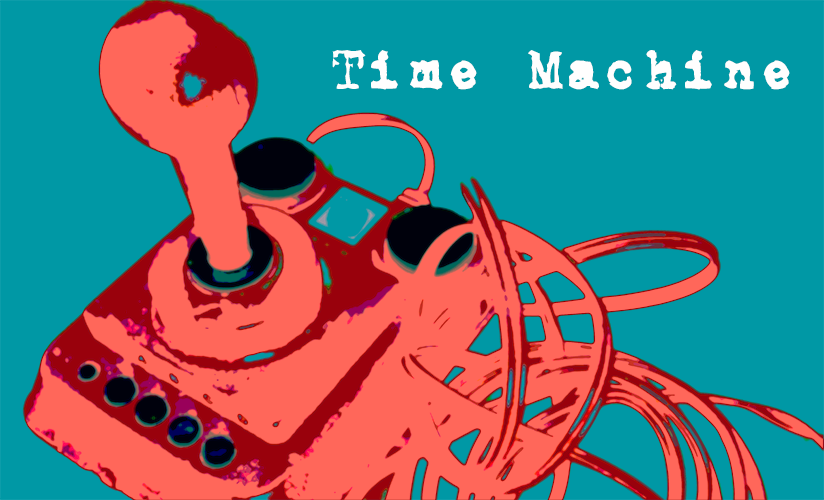
\includegraphics{Figures/02-02-TimeMachine} \end{center}

\textbf{Was steckt dahinter?}

Auch wenn es für gewöhnlich Wichtigeres im Leben gibt, als die technischen Dinge, so verändert der Kontakt mit ihnen doch unsere praktischen Handlungs- und Erfahrungsmöglichkeiten. Wir können plötzlich nach Informationen suchen oder uns in den Weiten des Internets verlaufen, wir können unseren Freund*innen Bilder und Nachrichten schicken, ohne dass es die anderen mitbekommen, oder wir entdecken uns bislang unbekannte Spiel- und Experimentierräume. Gleichzeitig entstehen damit aber auch neue Erwartungen an uns. Digital präsent zu sein wird plötzlich notwendig, um mit \textgreater dabei\textless{} zu sein, wir sollen den Computer nicht nur zum Spaß nutzen, sondern damit auch etwas \textgreater Sinnvolles\textless{} anstellen und bitte auch verantwortungsbewusst damit umgehen.

Wie sich der erste Kontakt mit digitalen Technologien gestaltet, ist dabei einerseits abhängig von unserer persönlichen Situation und dem sozialen Milieu, in der wir aufwachsen. Andererseits ist es aber auch eine Generationenfrage, ob bestimmte digitale Technologien, wie etwa Internet, Smartphone, Mähroboter, Google oder Messenger Dienste eigentlich immer schon da waren.

\chapter{Digitalisierung von Bildungsprozessen}\label{digitalisierung-von-bildungsprozessen}

Im Sinne eines kulturellen Transformationsprozesses hat die Digitalisierung einen tiefgreifenden Einfluss nicht nur auf die Art und Weise, wie wir lernen und uns bilden, sondern auch darauf, was wir unter Begriffen wie Lernen, Bildung, Wissen und Kompetenzen verstehen. In einer ersten Annäherung an die Frage nach der Digitalisierung von Bildungsprozessen geht es im Folgenden darum, einen ersten Überblick über verschiedene Perspektiven zu gewinnen, von dem aus sich entsprechende Transformationsprozesse betrachten und untersuchen lassen.

\begin{center}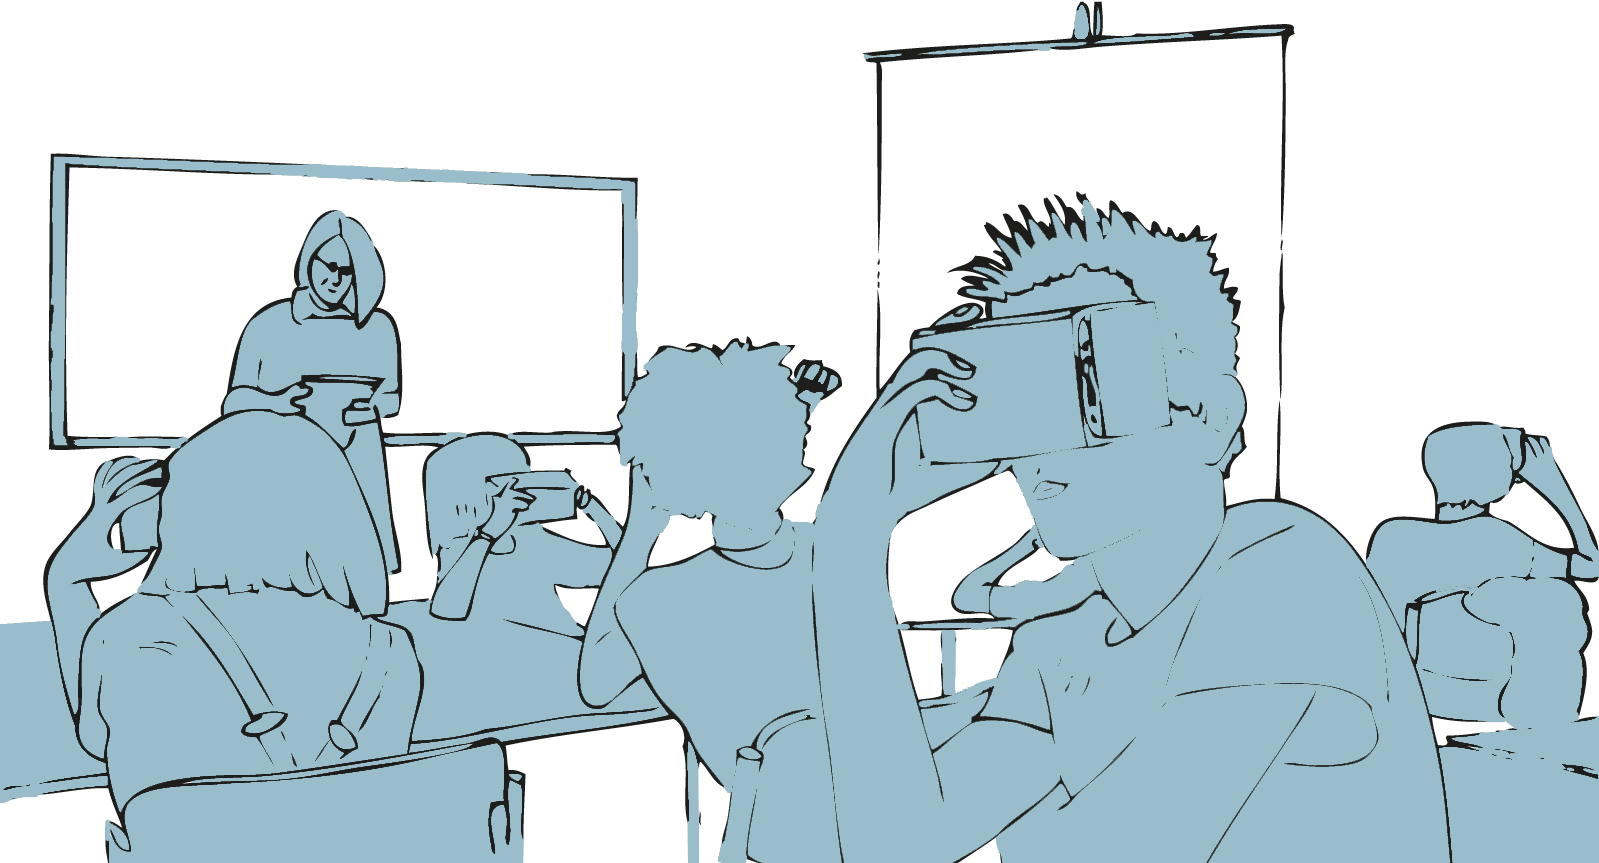
\includegraphics{Figures/03-01-Digitalisierung} \end{center}

\section{Lernen \& Bildung mit, über und durch digitale Medien}\label{lernen-bildung-mit-uxfcber-und-durch-digitale-medien}

In der aktuellen Diskussion um ›Bildung in der Digitalen Welt‹ wird die Frage nach der Digitalisierung von Bildungsprozessen aus verschiedenen Perspektiven verhandelt. Die hierbei vertretenen Positionen unterscheiden sich nicht zuletzt hinsichtlich der Rolle und Funktion, die den digitalen Technologien in Bezug auf Lernen und Bildung zugesprochen wird. Je nach Perspektive steht dabei die Vorstellung von Lernen und Bildung \textbf{mit, über oder durch digitale Medien} im Mittelpunkt der Betrachtung \citep{jorissenMedienbildungSatzen2013, othmerUndNochPaar2016}.

\textbf{Lernen \& Bildung mit digitalen Medien:}

Im Mittelpunkt dieser Perspektive steht die Vorstellung von digitalen Medien als Mittel, als Werkzeuge, Instrumente und Ressourcen, derer wir uns bedienen, um etwas zu lernen, uns zu bilden oder auch um andere zu unterrichten und Lernprozesse zu organisieren. Im Sinne von (Hilfs-)Mitteln liegt das Hauptaugenmerk aus dieser Perspektive auf dem effektiven und effizienten Einsatz digitaler Technologien und ihrem relativen Mehrwert gegenüber anderen Medien im Kontext von Lern- und Bildungsprozessen. Der gekonnte Umgang mit digitalen Medien und ihre zielgerichtete Verwendung sind entsprechend wesentliche Voraussetzungen für ihren produktiven Einsatz im Rahmen individueller Lernprozesse wie auch der Unterrichtsgestaltung.

\textbf{Lernen \& Bildung über digitale Medien:}

In Abgrenzung zu einem Lernen mit digitalen Medien richtet diese Perspektive den Blick auf digitale Medien als einen Gegenstand von Lern- und Bildungsprozessen. Digitale Medien treten hier vor allem als etwas in Erscheinung, über das wir etwas lernen können oder sollen. Ein solches Lernen über digitale Medien kann sich dabei sowohl auf deren technische Funktionsweise, ihre Entstehungsgeschichte, ihre soziale Bedeutung und Funktion wie auch Fragen eines angemessenen und in diesem Sinne kompetenten Gebrauchs beziehen. Neben der Befähigung zu einem praktischen Medienhandeln in privaten, öffentlichen und beruflichen Kontexten umfasst diese Perspektive auch den Erwerb der hierfür notwendigen Kenntnisse und Fertigkeiten.

\textbf{Lernen \& Bildung durch digitale Medien:}

Die dritte Perspektive wendet sich gegen die Vorstellung digitaler Medien als ›bloße‹ Mittel oder Gegenstände des Lernens oder der Bildung und betont stattdessen die mit der Verbreitung digitaler Medien einhergehende Transformation von Lebenswelten. Aus dieser Perspektive sind Digitale Medien ein integraler Bestandteil von Lern- und Bildungsprozessen. Sie bestimmen darüber mit, was unter den entsprechenden Prozessen überhaupt zu verstehen ist. Grundlage dieser Perspektive bildet ein starker Medienbegriff, der davon ausgeht, dass sich Medien »als eine Art Träger oder Stoff {[}verstehen lassen{]}, in dem sich bestimmte Vorgänge abspielen« \citep[S. 91]{meyerBildungNeuenMediums2014}. Digitale Medien durchdringen in diesem Sinne die Art und Weise, wie wir uns in der Welt bewegen, welche Erfahrungen wir machen, wie wir uns zu uns selbst aber auch zu unseren Mitmenschen verhalten, wie wir mit Wissen umgehen und uns organisieren. Siehe hierzu auch das gleichnamige Strategiepapier der Kultusministerkonferenz aus dem Jahr 2016 \citep{kultusministerkonferenzBildungDigitalenWelt2016}. Torsten Meyer \citep[S. 91]{meyerBildungNeuenMediums2014} verwendet zur Veranschaulichung das Beispiel der Fische, die im ›Medium‹ des Wassers leben. Medien sind in diesem Sinne etwas, in das wir quasi ›eingetaucht‹ sind und das uns, wie die Luft zum Atmen, oft erst dann bewusst wird, wenn es uns entzogen wird.

\section{Lernen \& Bildung im Kontext von Schule\ldots{}}\label{lernen-bildung-im-kontext-von-schule}

\textbf{\ldots mit digitalen Medien}

(Weiter-)Entwicklung und Veränderung von Lehrmitteln
bspw. digitale Schul- und Klassenbücher, interaktive Tafeln, intelligente tutorielle Systeme oder digitale Simulations- und Experimentalumgebungen

\textbf{\ldots über digitale Medien}

(Weiter-)Entwicklung von Unterrichtsinhalten bspw. in Form einer grundlegenden informatischen Bildung oder Angeboten zur Vermittlung digitaler Medienkompetenz der Digitalisierung als einem spezifischen Gegenstand

\textbf{\ldots durch digitale Medien}

regt zum Hinterfragen der Ideen von Lernen und Bildung an, die sich in digitalen Lernszenarien und Anwendungen realisieren und in Form heimlicher Lehrpläne wirksam werden \citep[z. B.][]{darvinYouthTechnologyHidden2019, decuypereResearchingEducationalApps2019, edwardsSoftwareHiddenCurriculum2015}.
Bis hin zur Frage wie eine derart umfassende Transformation von Lebenswelten überhaupt thematisiert und ein Verständnis für eine solche ›Kultur der Digitalität‹ \citep{stalderKulturDigitalitat2016} entwickelt werden kann

\begin{blackbox}
\textbf{Mit ›Antolin‹ betreibt der Schulbuchverlag Westermann unter \href{ttps\%20://antolin.westermann.de/}{https ://antolin.westermann.de/} eine populäre Plattform zur Leseförderung für die Primar- und Sekundarstufe I. Neben einem Überblick über die grundlegenden Funktionen und Zielsetzungen der Plattform durch den Verlag \citep{westermanngruppeAntolinProgrammZur2022} finden sich in der Literatur hierzu auch verschiedene kritische Analysen \citep{jornitzsieglindeMitAntolinPunkten2018, forschlerZurAmbivalentenWirkmachtigkeit2021}.}

\emph{Welches Modell, welche Idee von ›Lesen‹ realisiert sich in Antolin?}

\emph{Welche Aspekte des Lesens, der Bücher, der Leser*innen werden ausgeblendet?}

\end{blackbox}

\section{Minimale Leittexte}\label{minimale-leittexte}

\textbf{Ziel}

Minimale Leittexte dienen der eigenständigen Aneignung ausgewählter Methoden im Kontext des selbstorganisierten Lernens.

\textbf{Leitgedanke}

Minimale Leittexte versuchen die Beschreibung einer Methode auf das Wesentliche zu reduzieren und den Anwender*innen neue Handlungsmöglichkeiten zu erschließen. Die Methode geht von selbstorganisierten Lerner*innen aus, die die Verantwortung für ihr Handeln übernehmen, sich gegebenenfalls selbständig mit der Hintergrundliteratur befassen oder sich anderweitige Hilfe erschließen.

\textbf{Anwendungskontext}

Minimale Leittexte eignen sich für die Darstellung grundlegender Methoden in verschiedenen Anwendungsbereichen. Sie sind auf einen praxisorientierten Einstieg in die jeweilige Methode ausgerichtet und sollen die Anwender*nnen bei der Auswahl geeigneter Methoden unterstützen.

\begin{center}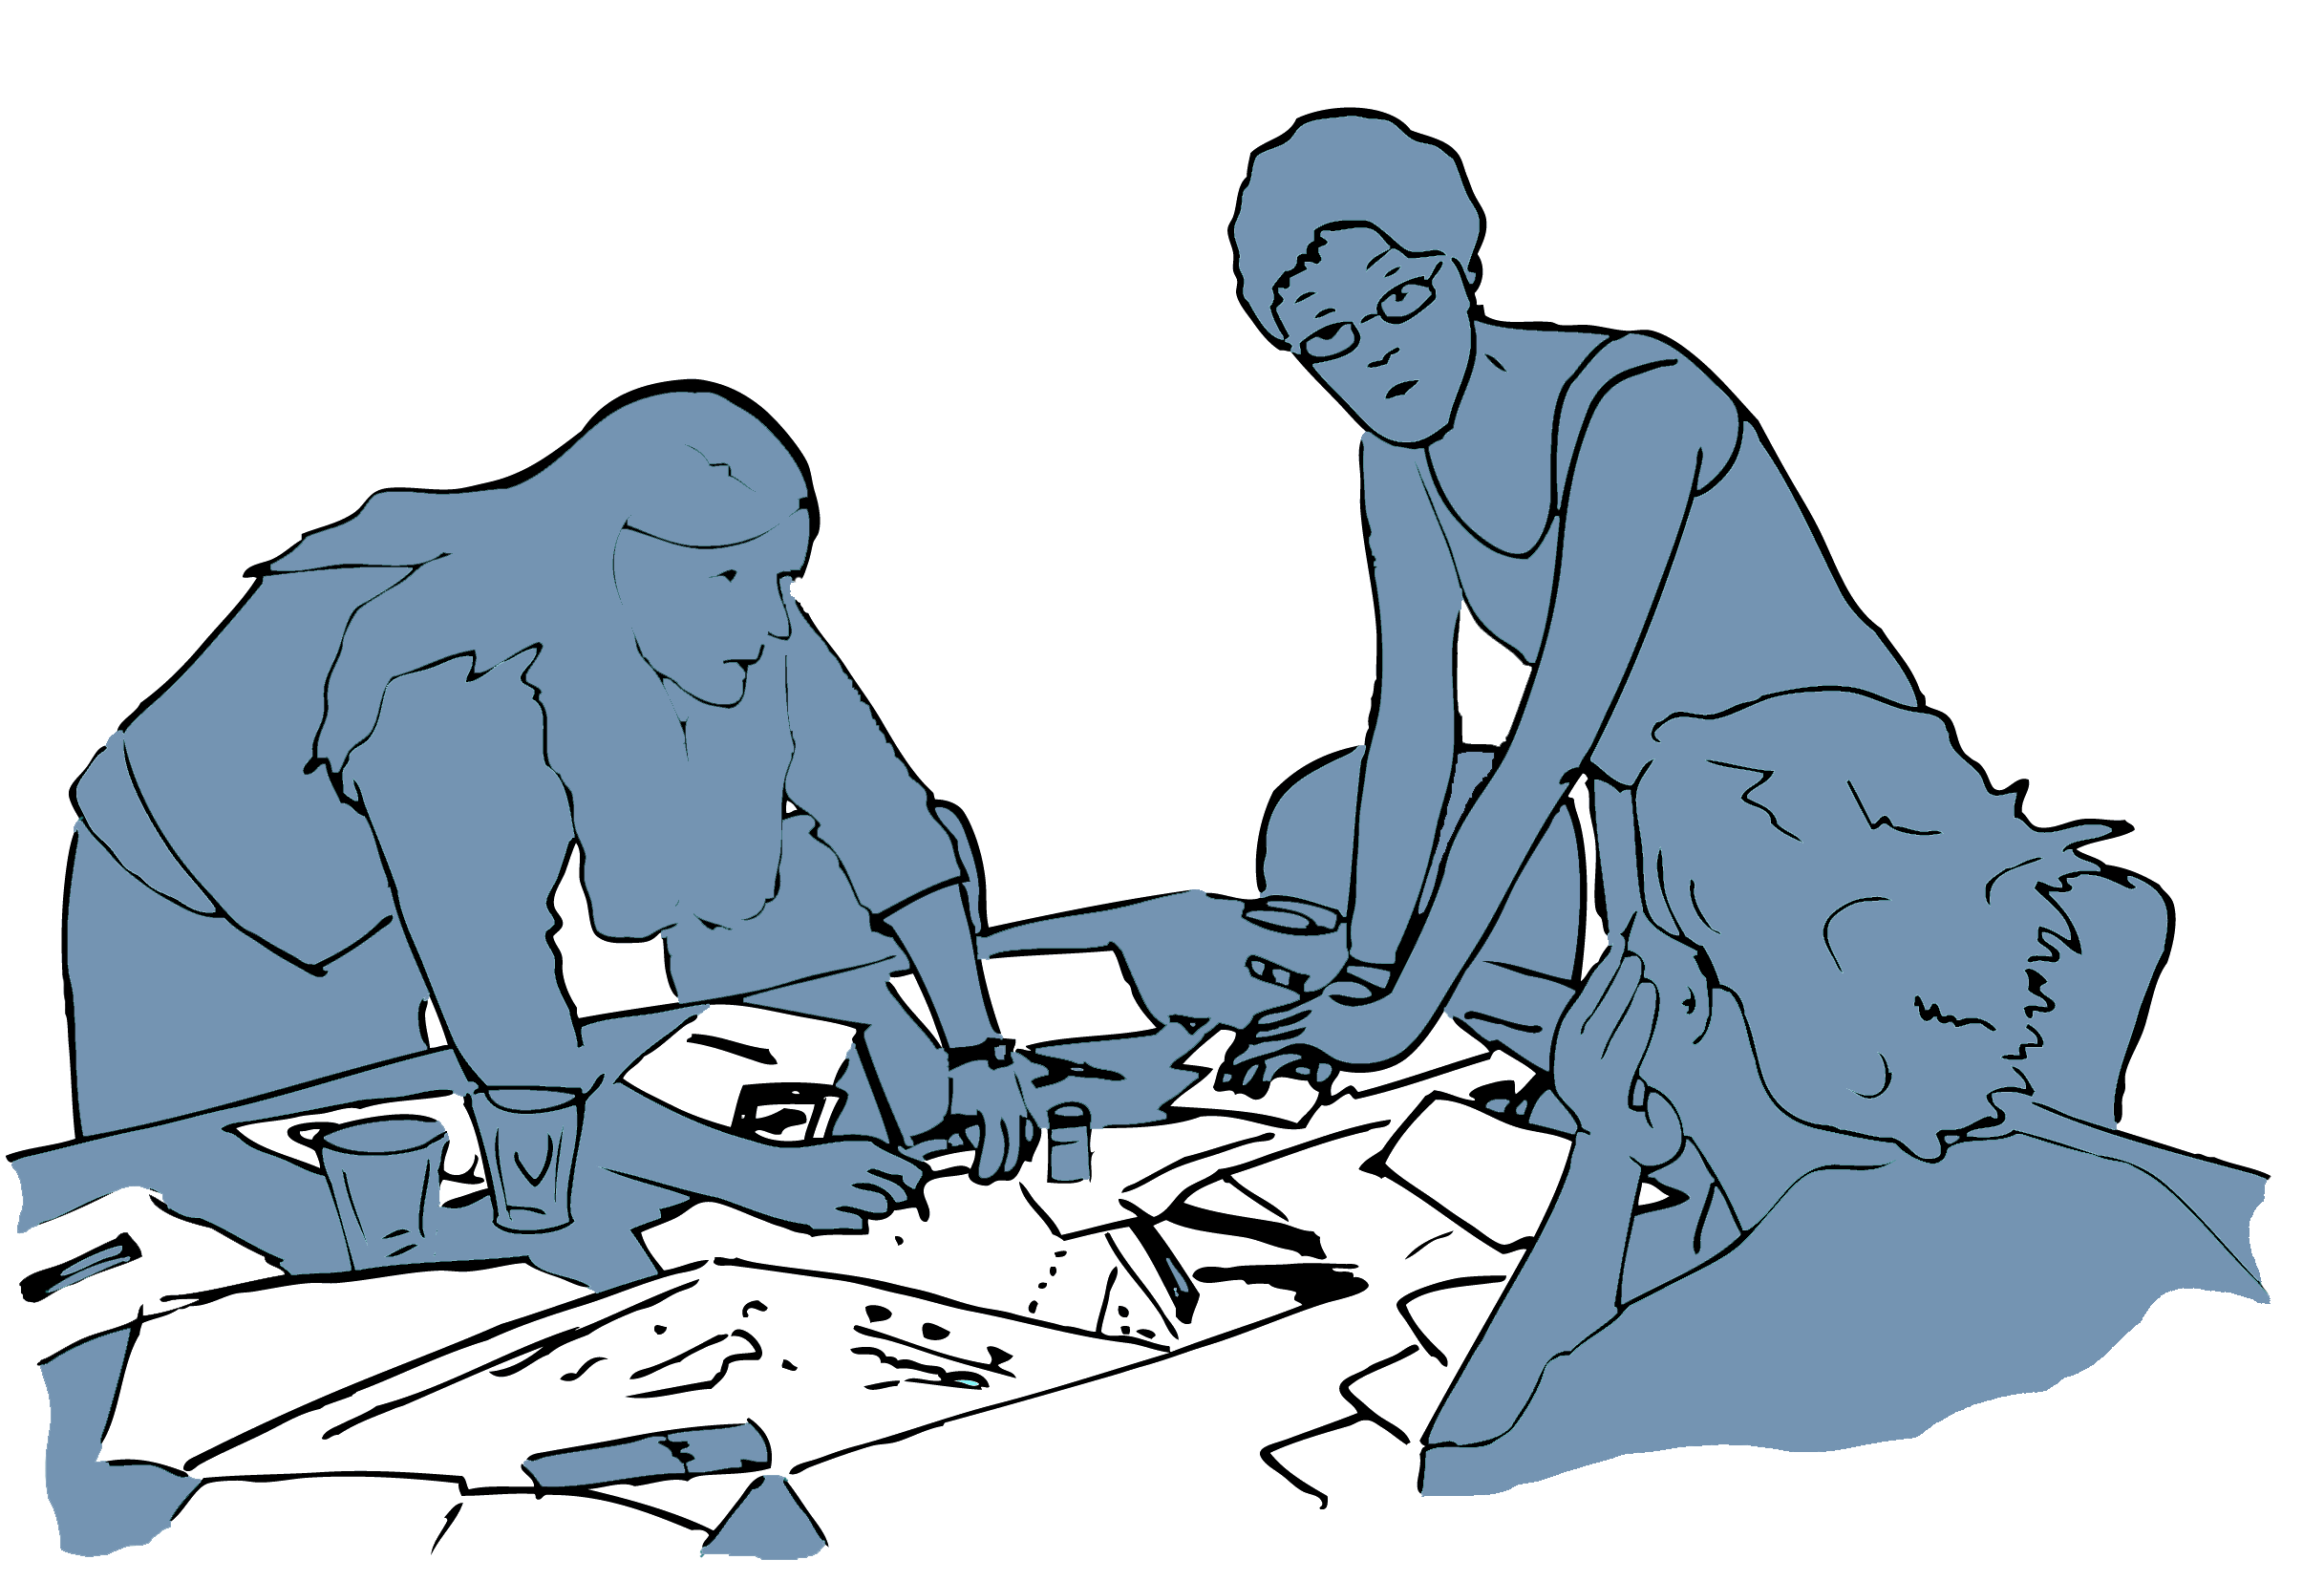
\includegraphics{Figures/03-02-praktik} \end{center}

\textbf{Arbeitsschritte}

\begin{enumerate}
\def\labelenumi{\arabic{enumi}.}
\tightlist
\item
  Die Erstellung minimaler Leittexte erfolgt in der Regel auf Basis einschlägiger Methodenliteratur und/oder auf den Erfahrungen des/der Autor*innen.
\item
  Minimale Leittexte werden entweder als Einzeldokumente oder in gesammelter Form potentiellen Anwender*innen zur Verfügung gestellt.
\item
  Die Leittexte werden auf Basis von Rückmeldungen durch die Anwender*nnen weiterentwickelt.
\end{enumerate}

\textbf{Ergebnisformat}

Das praktische Ergebnis ist der Minimale Leittext, bzw. ein entsprechender Pool von Leittexten.

\textbf{Praktische Tipps}

\begin{itemize}
\tightlist
\item
  Minimale Leittexte sollten auf das Wesentliche reduziert sein.
\item
  Die Beschreibung der Methode sollte aus sich heraus verständlich sein, sodass keine Verweise auf andere Dokumente notwendig sind.
\item
  Es sollten vor allem Methoden beschrieben werden, die sich in der Praxis bereits bewährt haben. Ist dies zum Beispiel bei einer neuen Methode nicht der Fall, so sollte dies im Leittext vermerkt werden.
\end{itemize}

\textbf{»Fallstricke«}

\begin{itemize}
\tightlist
\item
  Minimale Leittexte sind kein Ersatz für eine fundierte Methodenausbildung. Die methodologischen Grundlagen einer Methode können nur sehr bedingt dargestellt werden.
\item
  Minimale Leittext sind keine Kochrezepte, sie erfordern die aktive Interpretation und verantwortungsvolle Umsetzung durch den/die Leser*in.
\end{itemize}

\textbf{Weiterführende Literatur zum Leittext}

Greif, S. (1998)- Minimale Informations- und Leittexte. In: Greif, S., Kurtz H.-J. (Hrsg.). \emph{Handbuch Selbstorganisiertes Lernen} (S. 255-266). 2. Aufl.- Göttingen: Verlag für Angewandte Psychologie.

Richter, C., Allert, H., Nejdl, W. (2005). Minimal Activity Plans: Artifacts for Self-Organized Learning within Organizations. \emph{Proceedings of WM2005}, Kaiserslautern, Germany 2005. Bonn: Gesellschaft für Informatik, S. 166--169.

\chapter{Soziale Praktiken}\label{soziale-praktiken}

Eine der grundlegenden Fragen der Sozial- und Kulturwissenschaften, wie auch der Pädagogik, ist die nach dem Verhältnis von Mensch und Welt. Um dieses Verhältnis analytisch zu fassen, sind sehr unterschiedliche theoretische Positionen entwickelt worden. In Abgrenzung zu strukturtheoretischen, individualistisch-zweckrationalen und normorientierten Ansätzen haben in den letzten Jahrzehnten zunehmend kulturtheoretische Ansätze an Bedeutung gewonnen. Einer dieser Ansätze ist die \textbf{Theorie sozialer Praktiken}, die das Konzept \textbf{›sozialer Praktiken‹} zum Bezugspunkt theoretischer wie auch empirischer Überlegungen macht.

\begin{center}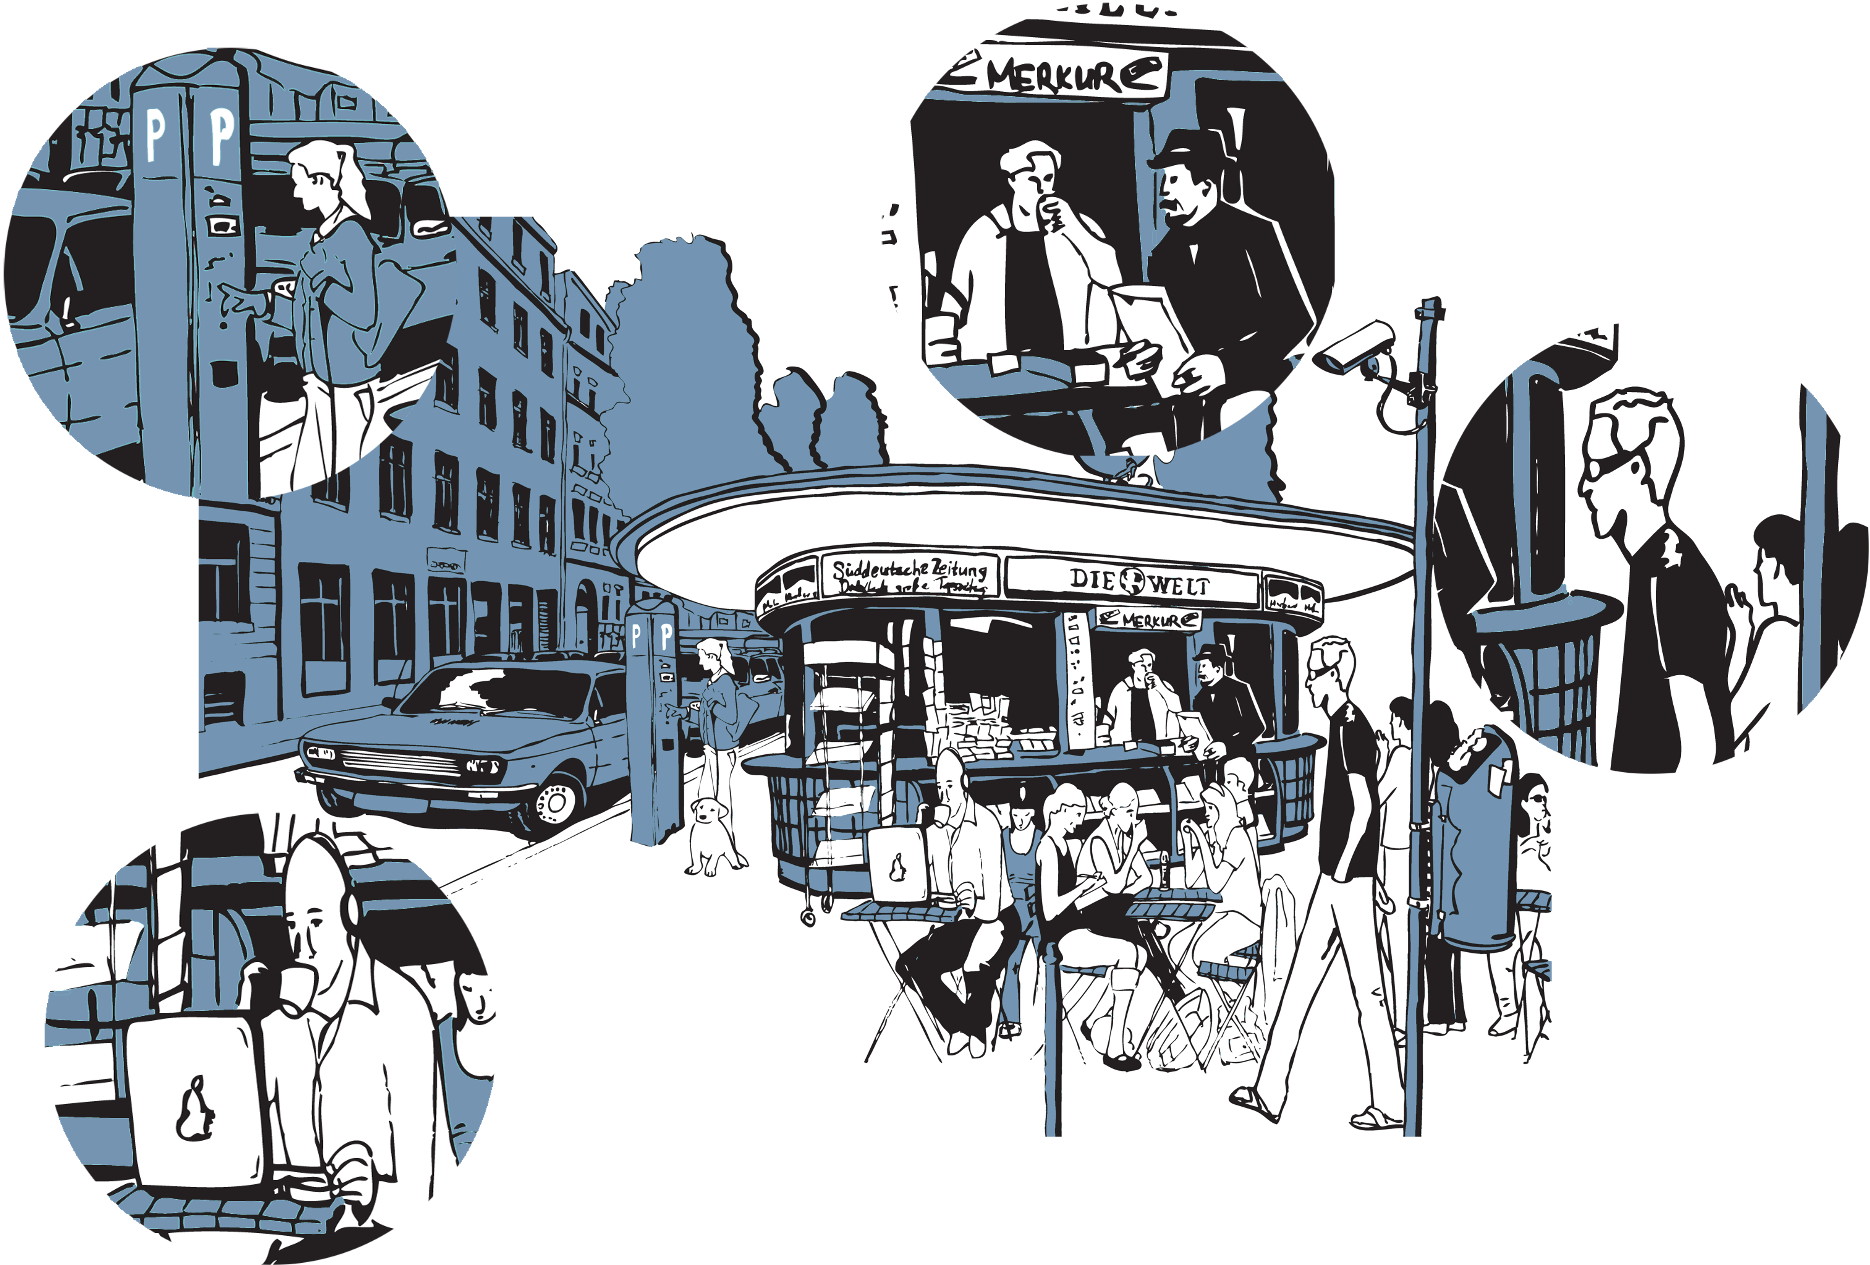
\includegraphics{Figures/04-01-Soziale-Praktiken} \end{center}

\section{Das Konzept der sozialen Praktik als analytischer Bezugspunkt}\label{das-konzept-der-sozialen-praktik-als-analytischer-bezugspunkt}

Die Begriffe ›Praktik‹ und ›Praxis‹ sind nicht nur im wissenschaftlichen, sondern auch im alltäglichen Sprachgebrauch weit verbreitet. Sie werden aber sehr unterschiedlich verwendet und sind oft nur vage definiert. So wird zum Beispiel der Begriff der Praxis dazu verwendet, um konkretes Handeln von theoretischen Betrachtungen zu unterscheiden. Mit Praxis kann aber auch die gesamte Lebenstätigkeit und die hiermit verbundenen Erfahrungen eines Menschen gemeint sein. Ebenso dient der Begriff der Praktik manchmal als Verweis auf eine allgemeine Methode oder Vorgehensweise, während in anderen Fällen die spezifische Art und Weise gemeint ist, auf die eine Person oder eine Gruppe von Personen etwas tut.

Im Rahmen der Theorie sozialer Praktiken werden Praktiken im Kern als eine organisierte Form menschlichen Tätigseins verstanden, in der sich »{[}d{]}urch häufiges und regelmäßiges Miteinandertun {[}\ldots{]} gemeinsame Handlungsgepflogenheiten heraus{[}bilden{]}, die sich zu kollektiven Handlungsmustern und Handlungsstilen verdichten und so bestimmte Handlungsvollzüge sozial erwartbar werden lassen« \citep{horningExpertenAlltags2001}. Soziale Praktiken sind in diesem Sinne kollektive Handlungsformen, die sich im Umgang von Menschen miteinander wie auch mit den Dingen ausbilden und sich im praktischen Tun kontinuierlich transformieren. Von diesem theoretischen Standpunkt aus sind soziale Praktiken der zentrale Bezugspunkt sowohl für soziale Phänomene, wie zum Beispiel Wissen, Macht, Institutionen und gesellschaftlichen Wandel, als auch für individuelle Prozesse, wie etwa des Denkens, der Identität, des Lernens und der Kommunikation \citep[vgl. z.B.][]{schatzkiPrimerPracticesTheory2012}.

Der Rückgriff auf praxistheoretische Positionen hat damit weitreichende Konsequenzen für das (medien-)pädagogische \textbf{Verständnis von Sozialisations-, Lern- und Bildungsprozessen}.

Prozesse der Sozialisation, des Lernens oder der Bildung lassen sich vor dem Hintergrund dieser Positionen nicht mehr losgelöst von den jeweiligen Praktiken, den kulturellen und technischen Milieus begreifen, in denen sie stattfinden. Der Fokus verschiebt sich damit \textbf{weg von der Annahme eines intentional handelnden und autonomen Subjekts hin zu den sozialen, kulturellen und technischen Beziehungsgefügen, in denen bestimmte menschliche Existenzweisen überhaupt erst ihre Form gewinnen und geformt werden} \citep[vgl. z.B.][]{fenwickEmergingApproachesEducational2011, munte-goussarMedienbildungSchulkulturUnd2016, richterBildungSchnittstelleKultureller2020}.

Prozesse der Sozialisation, des Lernens und insbesondere der Bildung lassen sich damit aber auch nicht nur als ›bloße‹ Anpassungen an bestehende soziale Ordnungen verstehen. Vielmehr eröffnen diese Positionen den Raum für eine Form von Subjektivität, in der Menschen die sich aus dem praktischen Handel ergebenden Potentiale nutzen können, um die bestehenden Ordnungen zu transformieren und neue Möglichkeiten für sich und andere zu erschließen \citep[vgl. z.B.][]{alkemeyerBefahigenPraxistheoretischeUberlegungen2017}.

\section{Wesentliche Ideen}\label{wesentliche-ideen}

\textbf{Praktiken erzeugen soziale Ordnungen} - Praktiken sind keine abstrakten Beschreibungen, sondern ein konkretes Produkt wiederholter Interaktionen und Kommunikationen (Doings und Sayings). Die Ausbildung von Praktiken reduziert die Komplexität sozialer Interaktionen, indem sie bestimmte Handlungsweisen nahelegen beziehungsweise erwartbar machen \citep[vgl. z.B.][]{bickhardSocialOntologyPersons2003, bickhardSocialOntologyConvention2008}. Praktiken können dabei in unterschiedlichem Maße institutionalisiert oder formalisiert sein.

\textbf{Praktiken setzen ›Know-How‹ und ein praktisches Verständnis der Akteur*innen voraus} - Jede Praktik folgt ihrer eigenen ›Logik‹. Diese Logik bestimmt nicht nur, welche Formen des praktischen Wissens relevant sind und welche funktionalen Erfordernisse zu beachten sind, sondern auch die normativen und ästhetischen Erwartungen, die an die Akteur*innen herangetragen werden \citep[vgl. z.B.][]{alkemeyerBefahigenPraxistheoretischeUberlegungen2017}. Die Logik einer Praxis realisiert sich vor allem im Miteinandertun. Die praktische Kompetenz der Akteur*innen ist deshalb neben der Kenntnis expliziter Regeln und der Einübung praktischer Vorgehensweisen vor allem die Fähigkeit zur produktiven Interaktion mit anderen Praktiker*innen.

\textbf{Praktisches Handeln ist ein situationsgebundener Prozess} - Praktisches Handeln wird weniger durch unsere Pläne und Ideen bestimmt als durch die Anforderungen und Möglichkeiten, denen die Akteur*innen begegnen. Praktisches Handeln ist kein in sich abgeschlossener oder wiederholbarer Akt, sondern vielmehr ein fortlaufenderProzess, in dem Menschen sich der ihnen verfügbaren Ressourcen bedienen, um die Situationen, in denen sie sich befinden, zu verstehen und mit ihnen umzugehen \citep[vgl. z.B.][]{horningSozialePraxisZwischen2004}. Menschliches Handeln vollzieht sich insofern immer im Rahmen praktischer Erwartungs- und Möglichkeitshorizonte.

\textbf{Soziale Praktiken sind in der materiellen Welt verankert} - Im Sinne konkreter Aktivitäten nehmen soziale Praktiken immer auch auf die materielle Welt Bezug. Dies gilt sowohl für die Körper der Akteur*innen, die physischen Umwelten, in denen sie agieren, wie auch für die (technischen) Artefakte, die im Rahmen der Praktiken verwendet oder hergestellt werden. Sowohl die Körper, die physischen Umwelten wie auch die (technischen) Artefakte sind dabei in vielen Fällen sowohl Voraussetzung wie auch das Produkt der jeweiligen sozialen Praktiken \citep[vgl. z.B.][]{schatzkiPrimerPracticesTheory2012}.

\textbf{Praktiken existieren in einem eigentümlichen Spannungsverhältnis aus Stabilität und Veränderung} - Indem soziale Praktiken Komplexität reduzieren und Erwartbarkeit schaffen, erzeugen sie immer auch ein bestimmtes Maß an Stabilität. Da sich praktisches Handeln aber in immer wieder neuen Situationen vollzieht, kann sich praktisches Handeln nicht allein in der Wiederholung des schon Dagewesenen erschöpfen. Vielmehr setzt praktisches Handeln immer auch eine produktive Auseinandersetzung und eine Erschließung des noch Unbekannten voraus \citep[vgl. z.B.][]{horningSozialePraxisZwischen2004}.

\begin{blackbox}
\emph{Welche sozialen Praktiken lassen sich im Kontext von Schule ausmachen?}

\emph{Wie lassen sich diese charakterisieren?}

\end{blackbox}

\begin{center}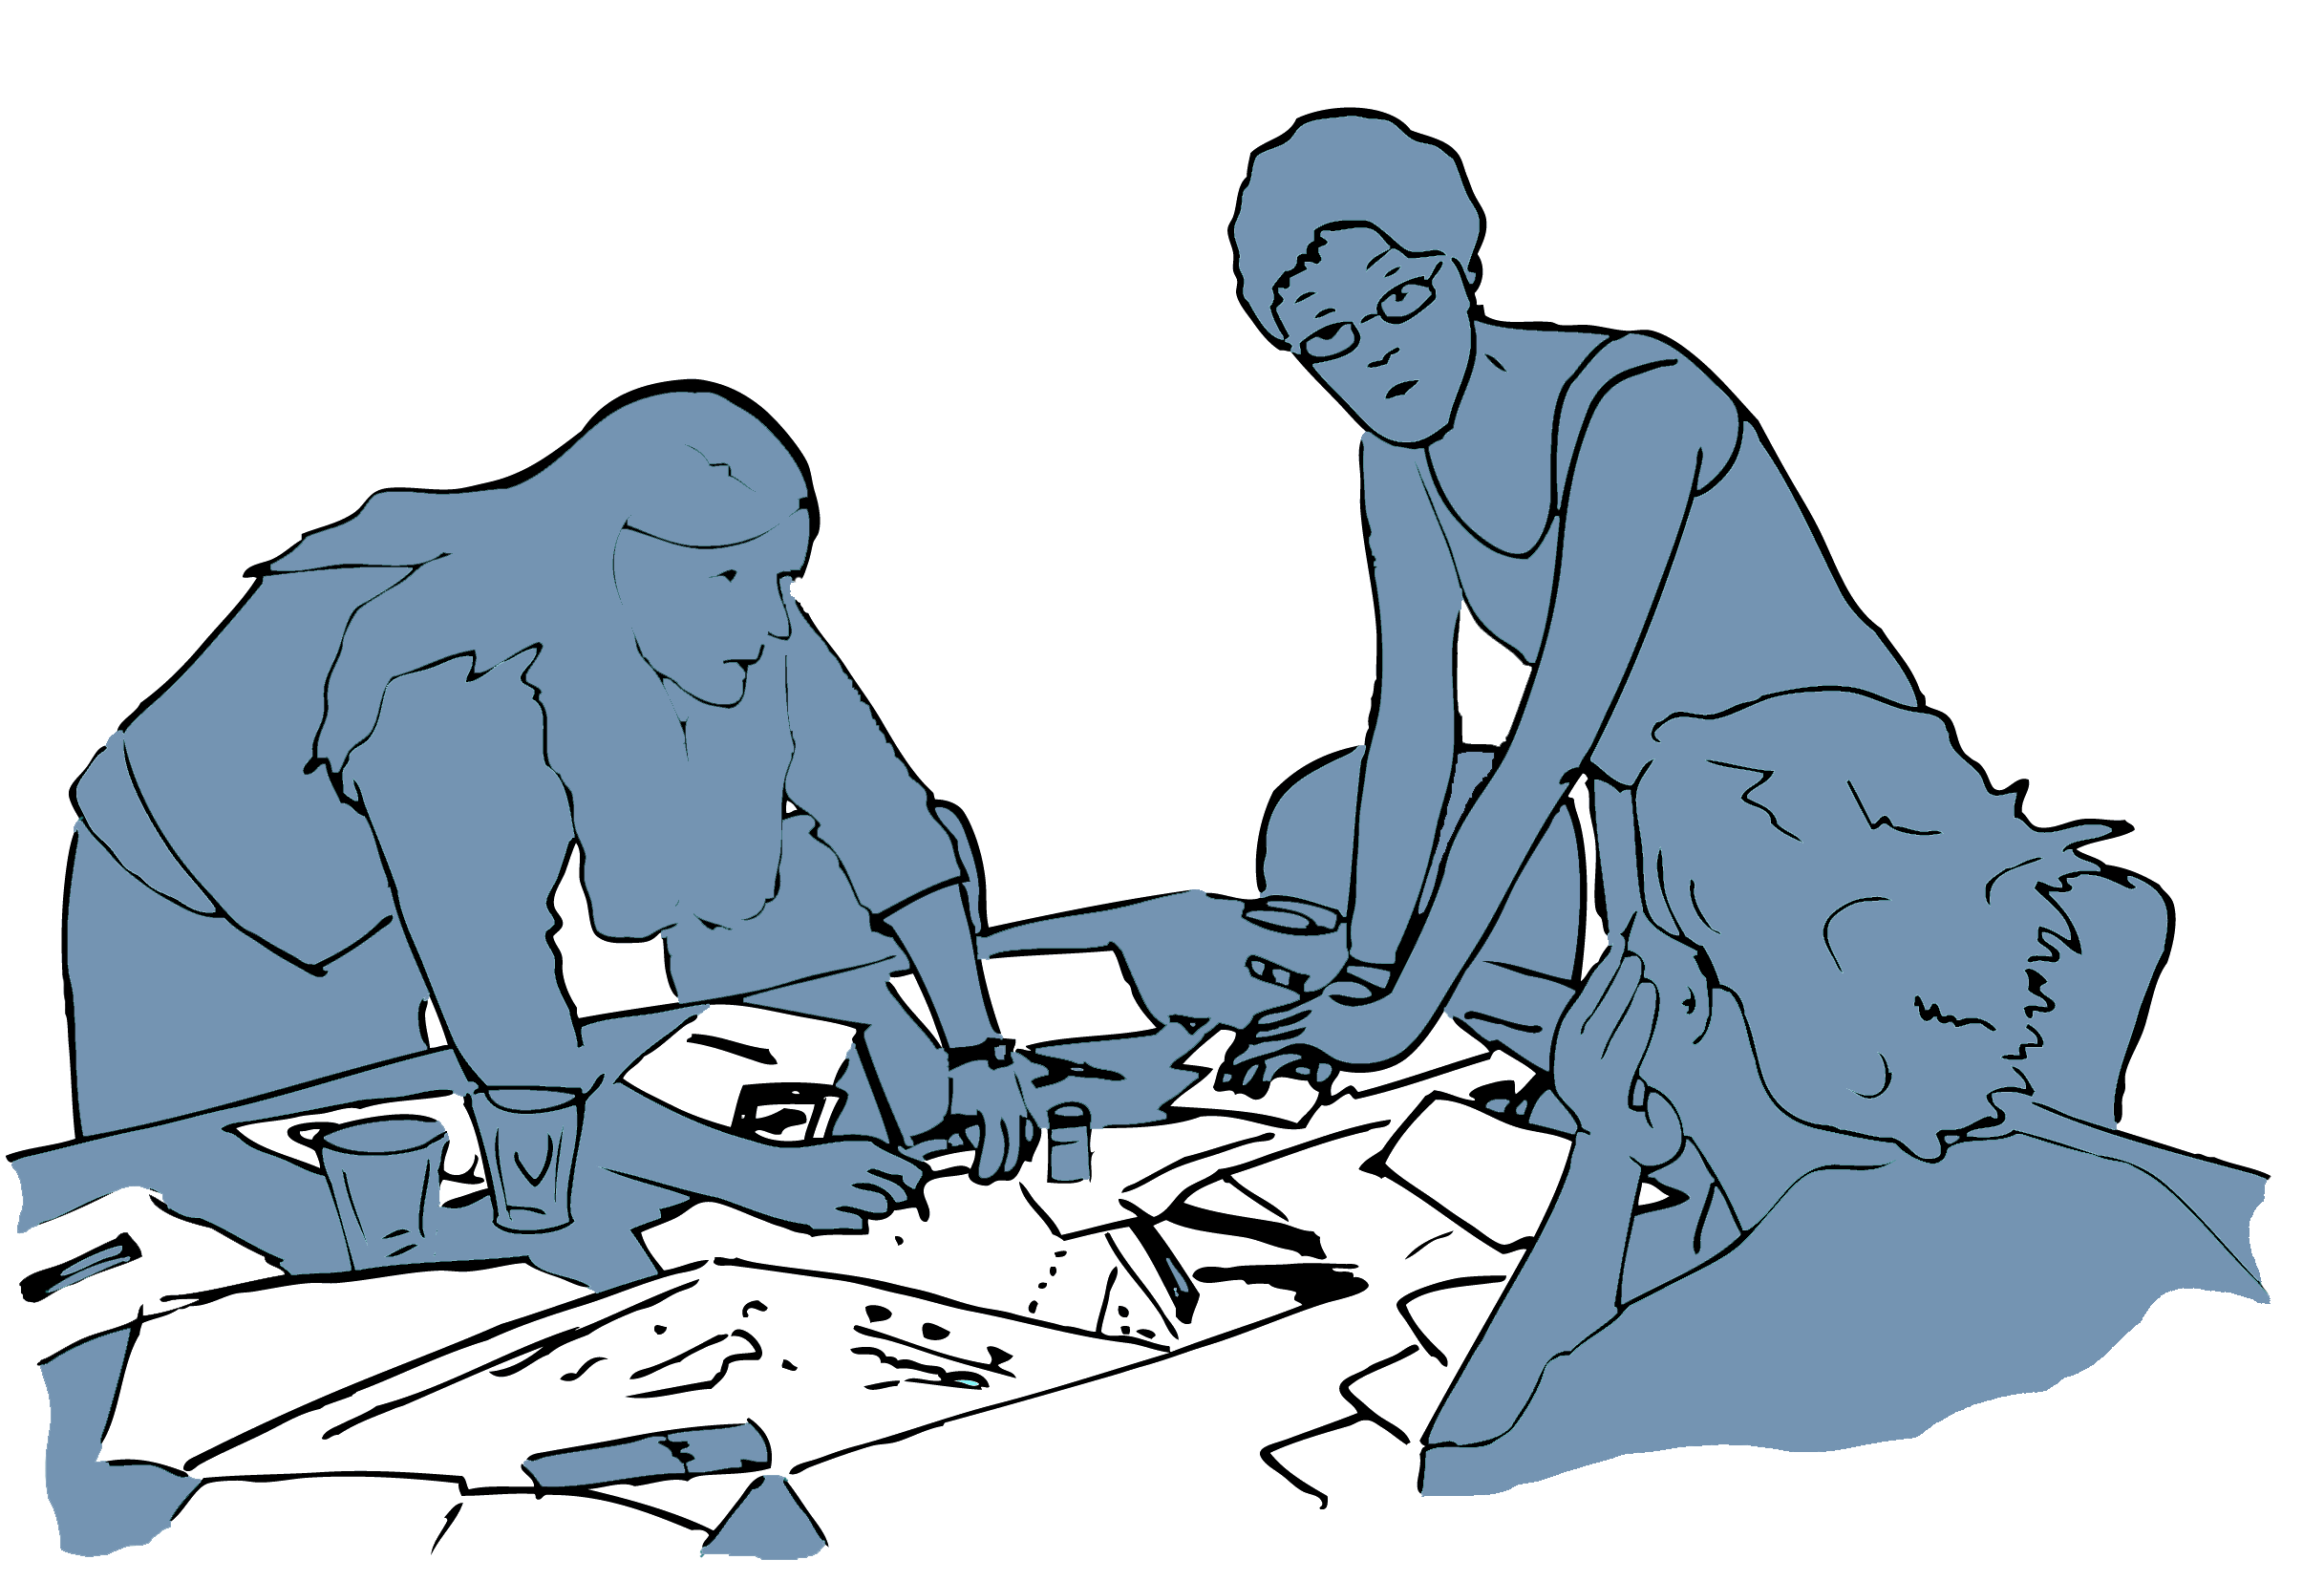
\includegraphics{Figures/03-02-praktik} \end{center}

\section{Mein Lernkosmos}\label{mein-lernkosmos}

\emph{(Autorin: Helena Hintz)}

Wann und wo hast du in deiner Kindheit und Jugend etwas für dich Bedeutsames gelernt? Welche Umgebungen und Bedingungen waren dabei besonders gute Nährböden für diese Lernerfahrungen? Gestalte einen persönlichen Lernkosmos in Form einer Karte, in welchem du für dich wesentliche Lernerfahrungen visualisierst und verortest.

\textbf{Worum geht`s?}

Oft sind es in unserer Kindheit und Jugend Gegebenheiten außerhalb von Schule, die uns zum (schulischen) Lernen animieren. Der Frankreich-Austausch in der 8. Klasse, der die Liebe für die Sprache weckt. Der Besuch im Aquarium, nach dem man mehr über Wasserlebewesen lernen möchte. Die Begeisterung fürs Backen oder die Möglichkeit, sich in Computer zu hacken. Aber auch innerhalb der Schule kann uns die begeisterte Lehrkraft zur Liebe für Gedichte oder die Robotik-AG zur Auseinandersetzung mit Technik animieren.

Verschiedene Kontexte und Impulse können die Begeisterung in uns erwachen lassen und zu bedeutsamen Lernerfahrungen führen. Wann haben wir uns also animiert gefühlt, Neues zu lernen? Wo befinden sich diese Orte in unserem individuellen Lernkosmos?

\begin{center}
\includegraphics{Figures/04-03-Lernkosmos} \end{center}

\textbf{Was steckt dahinter?}

Spätestens mit dem Kontakt zur Schule verbinden viele Lernen mit bestimmten Unterrichtsfächern. Manche Kinder gehen in dem System auf, andere gehen unter. Dabei wird oft vergessen, dass Lernen in vielen Kontexten stattfinden kann, von denen Schule nur einen Teil darstellt. Für viele Schüler*innen kann es ein Unterrichtsfach oder eine Lehrkraft sein, die Begeisterung für Themen entfacht, Lernerfahrungen gehen jedoch zumeist über die Grenze des Schulgeländes hinaus.

Etwas zu lernen kann sich durch Begeisterung, Notwendigkeit oder ganz nebenbei entwickeln -- wird oft aber nicht als Lernen wahrgenommen. Eigene Lernerfahrungen zu kartographieren, sich bewusst mit ihnen auseinanderzusetzen, kann dazu führen, dass plötzlich nicht mehr die Schule als Ort des Lernens im Mittelpunkt steht. Was macht das mit dem Verständnis der Schule als primärer Lernort?

~

\begin{licencebox}{licencebox}
Der Impuls ›Mein Lernkosmos‹ wurde 2022 von \href{mailto:hel.hintz@gmail.com}{Helena Hintz} erstellt und ist unter einer Creative Commons \href{https://creativecommons.org/licenses/by-sa/4.0/}{CC BY-SA 4.0} Lizenz veröffentlicht.

\end{licencebox}

\chapter{Soziale Praktik \& Technik}\label{soziale-praktik-technik}

Technik ist ein integraler Bestandteil unseres alltäglichen Handelns und damit auch unserer sozialen Praktiken. Egal ob wir mit dem Fahrrad zur Arbeit fahren, am Computer einen Text schreiben, unser Essen in der Mikrowelle aufwärmen oder in unserer Freizeit Klavier spielen, immer wieder haben wir es mit den verschiedensten technischen Geräten, Instrumenten und Maschinen zu tun. Die Frage, was eine Technik eigentlich ist und welche Bedeutung dem Gebrauch technischer Dinge zukommt, wird aber weiterhin kontrovers diskutiert. Diese Diskussion erstreckt sich dabei von der Technikphilosophie über die Techniksoziologie bis hinein in die Kulturwissenschaften. Einen einführenden Überblick über verschiedene theoretische Positionen gibt unter anderem Werner Rammert \citep{rammertTechnik2010}. Eine ausführliche Darstellung grundlegender technikphilosophischer Diskurse findet sich zum Beispiel bei Carl Mitcham \citep{mitchamThinkingTechnologyPath1994}.

\begin{center}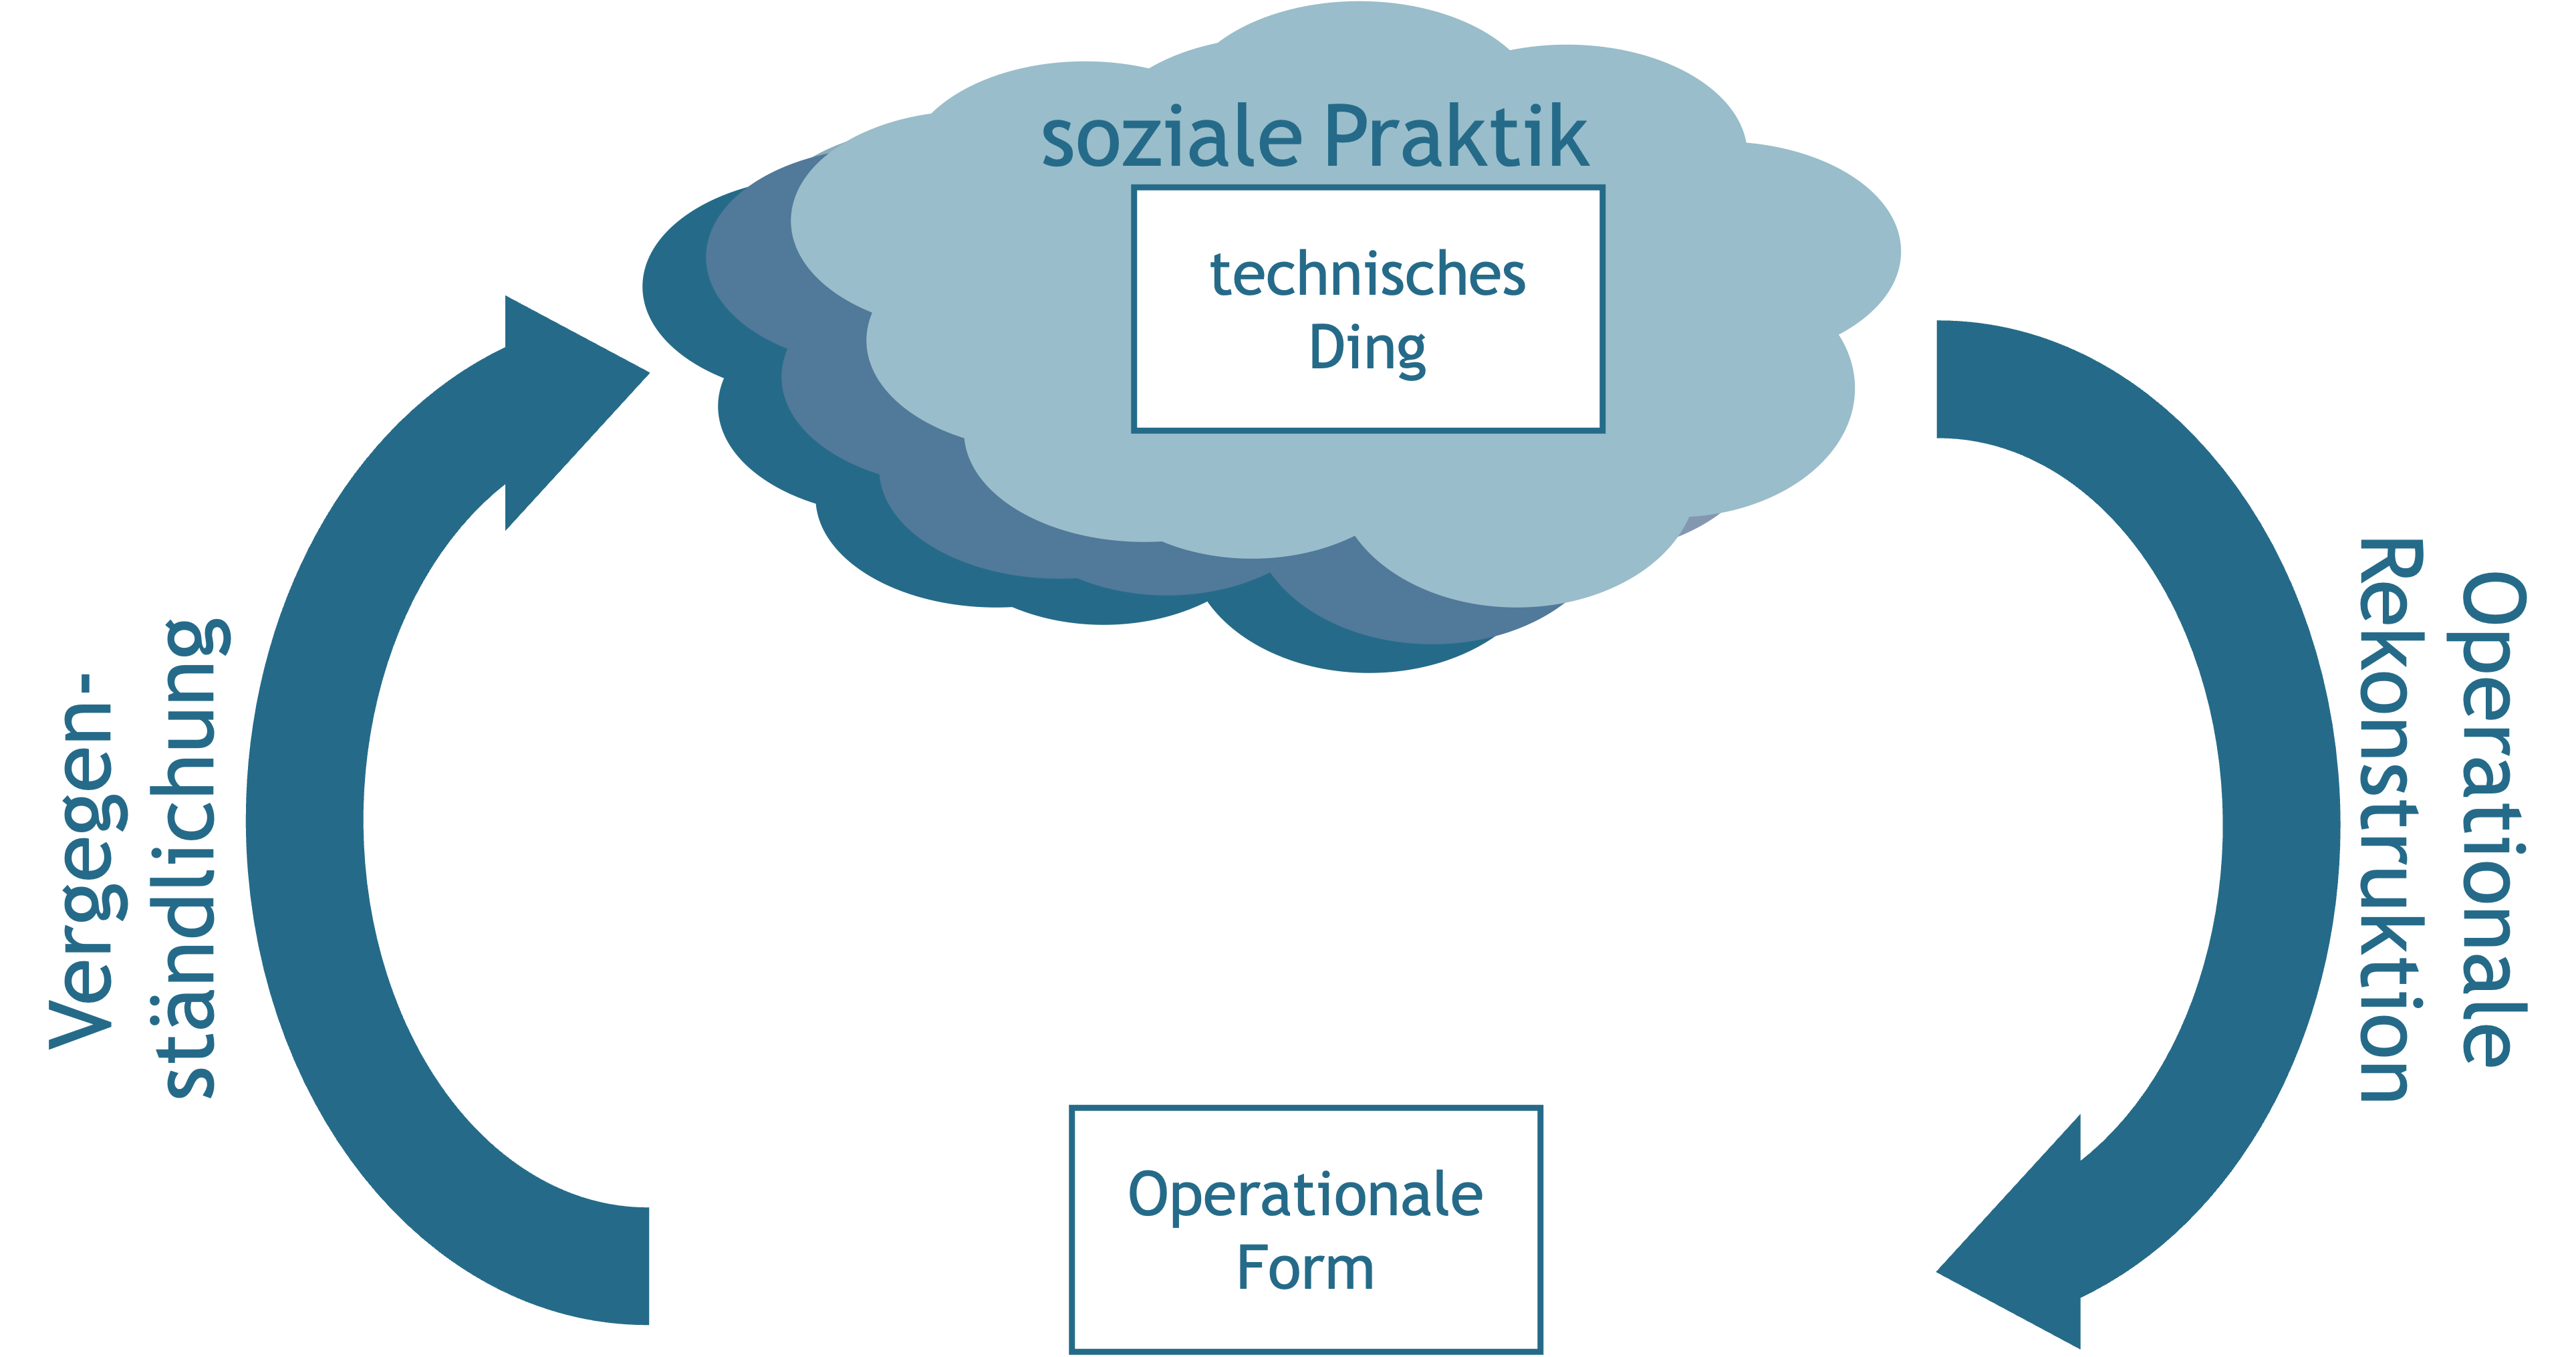
\includegraphics{Figures/05-01-SozialePraktik} \end{center}

\section{Das Konzept der Technik}\label{das-konzept-der-technik}

Die besondere Herausforderung in Bezug auf das Konzept der Technik besteht darin, dass mit dem Begriff der ›Technik‹ mindestens drei verschiedene Bedeutungsebenen verbunden sind \citep{mitchamThinkingTechnologyPath1994, horningExpertenAlltags2001}. So verweist der Begriff der Technik einerseits auf eine bestimmte Art von \textbf{Gegenständen}, die sich dadurch auszeichnen, dass sie von Menschen erschaffen worden sind und aufgrund ihrer materiellen Beschaffenheit bestimmte Wirkungszusammenhänge absichern. Andererseits bezeichnet der Begriff der Technik aber auch \textbf{Verfahren, Prozeduren und Fertigkeiten}, die Menschen (unter Verwendung technischer Dinge) erlernen und ausführen können. Beispiele hierfür sind etwa Moderations-, Unterrichts- oder Rechentechniken. Darüber hinaus kann Technik, im Sinne von ›Technologie‹, aber auch als eine \textbf{Form des Wissens} über technische Zusammenhänge verstanden werden.

Während sich die technischen Dinge für gewöhnlich recht einfach identifizieren lassen, da sie uns meist in Form konkreter Gegenstände, wie etwa dem Fahrrad, dem Computer, der Mikrowelle oder dem Klavier begegnen, ist die Frage nach der praktischen Funktion und Bedeutung dieser Dinge deutlich schwieriger zu beantworten. Ist zum Beispiel das Fahrrad ein Transportmittel, ein Sportgerät, ein Bastelobjekt, ein Beitrag zu einer nachhaltigeren Mobilität oder ein Zeichen dafür, dass man sich kein Auto leisten kann?

Während in den Sozial- und Kulturwissenschaften weitgehende Einigkeit darüber herrscht, dass technische Dinge das Ergebnis sozialer beziehungsweise kultureller Prozesse sind, unterscheiden sich die theoretischen Ansätze insbesondere hinsichtlich der Frage, ob die Funktion und Bedeutung der technischen Dinge Ausdruck der Intention derjenigen ist, die die technischen Dinge herstellen, oder ob sich die Funktion und Bedeutung der technischen Dinge erst im Gebrauch entscheidet \citep{orlikowskiUsingTechnologyConstituting2000}.

Vertreter*innen der Theorie sozialer Praktiken betonen den Umstand, dass technische Dinge keine austauschbaren Werkzeuge sind, sondern vielmehr einen \textbf{grundlegenden Bestandteil der jeweiligen Praktiken} darstellen. Technische Dinge sind dabei sowohl Voraussetzung wie auch Produkt sozialer Praktiken. In den technischen Dingen vergegenständlichen sich ›operationale Formen‹ \citep{floydAutooperationaleFormUnd1997}, die sich im Laufe des wiederholten Miteinandertuns herausgebildet haben.

Die Theorie sozialer Praktiken hebt dabei die konstitutive Verschränkung von sozialen Praktiken und technischen Dingen hervor, die sich in einem co-evolutionären Prozess gegenseitig bedingen und kontinuierlich transformieren \citep{mitchamThinkingTechnologyPath1994, shoveDynamicsSocialPractice2012}. Die Funktion und Bedeutung technischer Dinge muss dementsprechend immer wieder praktisch hergestellt werden; die technischen Dinge sind nicht schon von sich aus wirksam, sondern müssen ›ins Laufen‹ gebracht und auch ›am Laufen gehalten‹ werden. Hierzu braucht es sowohl die entsprechenden Fertigkeiten wie auch das Wissen der Praktiker*innen.

\section{Wesentliche Ideen}\label{wesentliche-ideen-1}

\textbf{Technische Dinge sind Voraussetzung und Produkt sozialer Praktiken} - Technische Dinge entwickeln ihre Form im Wechselspiel von Konzeption, Herstellung und Gebrauch. Die Vorstellungen der Entwickler*innen und die Erwartungen der Praktiker*innen sind dabei wechselseitig aufeinander bezogen. Mit der Einführung neuer technischer Dinge verändern sich die praktischen Handlungsspielräume, gleichzeitig entstehen aber auch neue Handlungsnotwendigkeiten und Erwartungen, die wiederum Anlass geben für die Weiterentwicklung der technischen Dinge \citep{shoveDynamicsSocialPractice2012}.

\textbf{Technische Dinge sind praktisch unterbestimmt} - Als Gegenstände können technische Dinge im Rahmen unterschiedlicher Praktiken Verwendung finden. Technische Dinge sind hinsichtlich ihrer praktischen Einsatzmöglichkeiten mehr oder weniger unterbestimmt. Während in einigen Fällen technische Dinge für spezifische Kontexte entwickelt werden, sind viele technische Dinge so konzipiert, dass sie in unterschiedlichen Kontexten Anwendung finden können. Neben einer geplanten Anpassbarkeit besteht dabei immer auch die Möglichkeit praktischer Zweckentfremdungen und Umnutzungen \citep{brandesNonIntentionalDesign2006, houkesOntologyArtefactsHard2006}.

\textbf{Technische Dinge haben eine materielle Form} - Technische Dinge sind keine abstrakten Objekte, sondern konkrete Gegenstände, mit denen im praktischen Gebrauch interagiert und hantiert werden kann. Aufgrund ihrer materiellen Eigenschaften sind die technischen Dinge nicht beliebig (um-)formbar, sondern immer auch eigensinnig beziehungsweise widerständig \citep{houkesOntologyArtefactsHard2006, kalthoffEinleitungMaterialitatKultur2016}. Für ihre Herstellung wie auch für ihre Wartung und Reparatur bedarf es bestimmter Fertigkeiten, Kenntnisse und gegebenenfalls weiterer (technischer) Dinge. Der Einsatz technischer Dinge erfordert zudem für gewöhnlich die Verfügbarkeit bestimmter Ressourcen, die verbraucht, benötigt oder bearbeitet werden, wie auch von Infrastrukturen, die die Verfügbarkeit der Ressourcen sicherstellen \citep{shoveMattersPractice2017}.

\textbf{Technische Dinge integrieren technische Elemente} - Technische Dinge setzen sich für gewöhnlich aus unterschiedlichen technischen Elementen zusammen, die zu einem bestimmten Zeitpunkt in einer Kultur verfügbar sind. Technische Elemente sind dabei grundlegende Prinzipien und Verfahren, die in die Konstruktion technischer Dinge einfließen und deren technische Eigenschaften und Funktionsweisen gewährleisten \citep{simondonExistenzweiseTechnischerObjekte2012}. Die Entwicklung technischer Elemente geht der Konstruktion und Herstellung konkreter technischer Dinge zumeist voraus.

\textbf{Technische Dinge bedürfen entsprechender soziotechnischer Milieus} - Damit technische Dinge praktisch einsetzbar werden, bedarf es hierauf abgestimmter sozialer und technischer Milieus. Neben der Verfügbarkeit geeigneter Ressourcen, Infrastrukturen und Produktionsbedingungen bedarf es entsprechender Fertigkeiten und Kenntnisse der beteiligten Akteur*innen wie auch sozial geteilter Deutungs- und Handlungsmuster, die den Einsatz bestimmter technischer Dinge sinnhaft erscheinen lassen. Die Entwicklung technischer Dinge geht insofern immer auch mit der Ausbildung entsprechender Milieus einher.

\begin{blackbox}
\emph{Welche analogen \& digitalen Technologien haben unseren Alltag nachhaltig verändert?}

\end{blackbox}

~

\begin{center}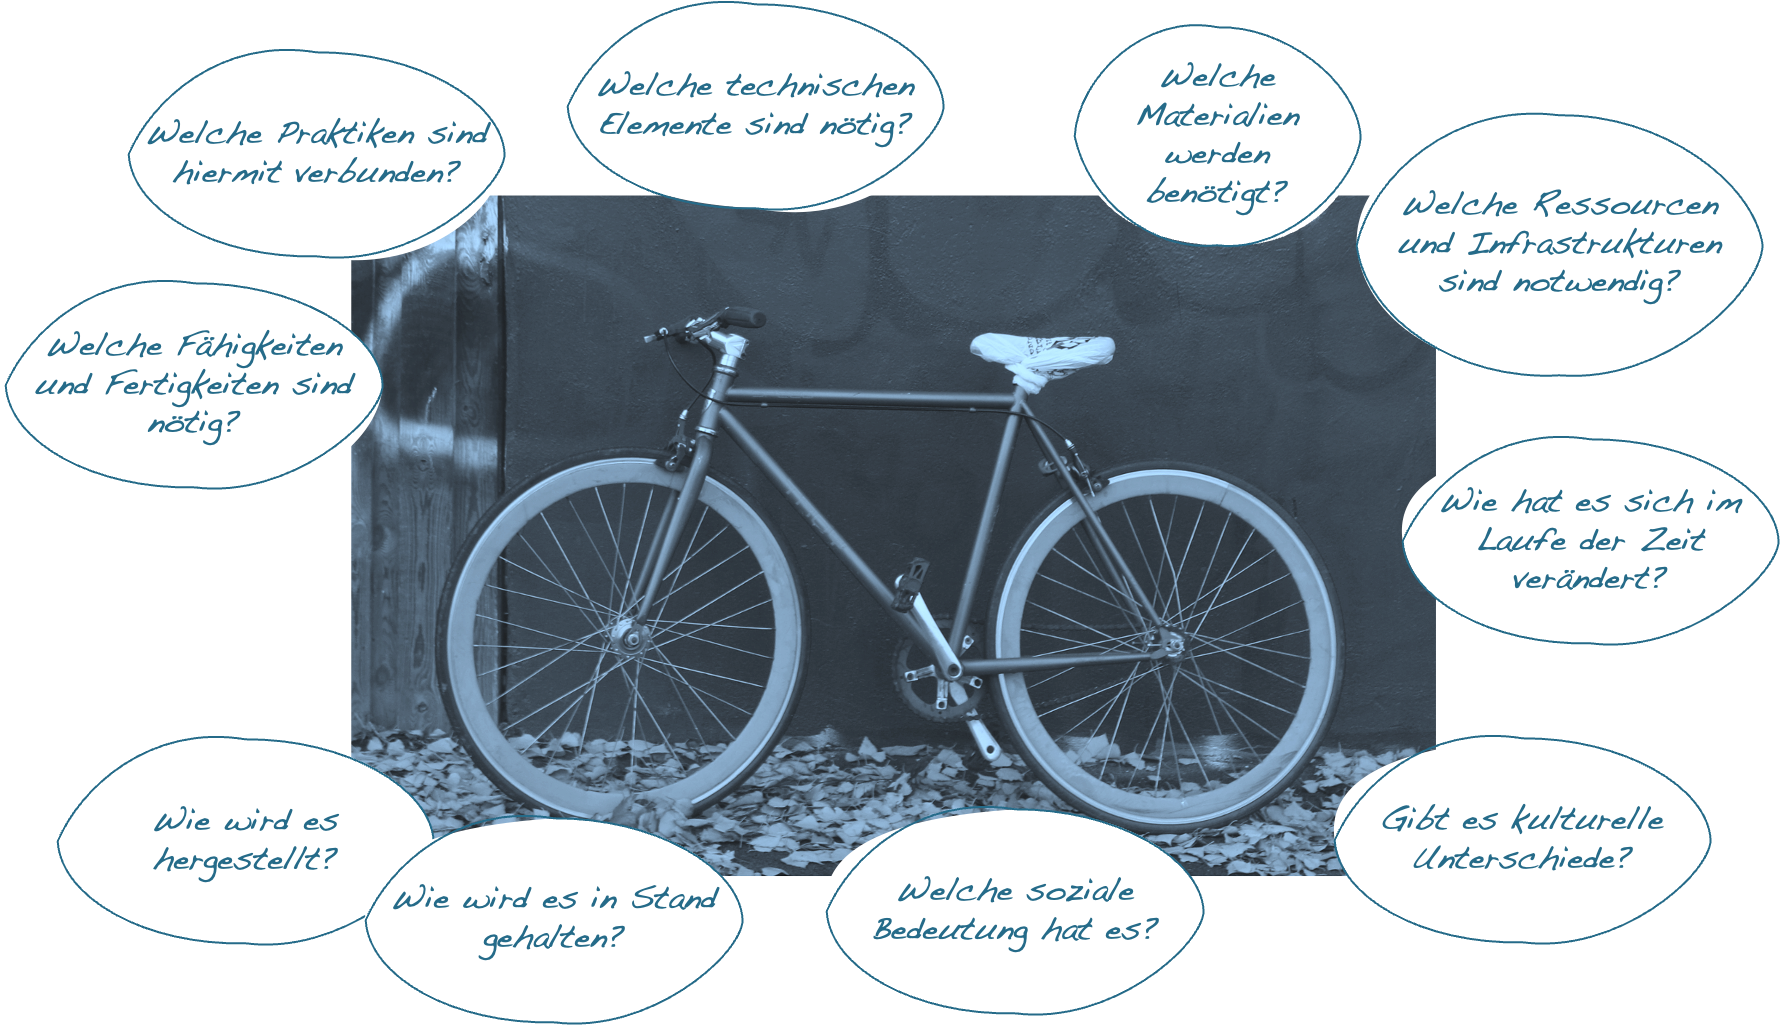
\includegraphics{Figures/05-02-Fahrrad} \end{center}

\section{Kartierung Sozialer Praktiken}\label{kartierung-sozialer-praktiken}

\textbf{Ziel}

Die Kartierung sozialer Praktiken dient der analytischen Abgrenzung praktischer Handlungszusammenhänge sowie die Identifikation wesentlicher Strukturelemente.

\textbf{Leitgedanke}

Die Kartierung sozialer Praktiken versucht organisierte Formen menschlichen Tätigseins zu identifizieren und gegeneinander abzugrenzen. Es geht hierbei darum, sowohl wesentliche Strukturelemente einer Praktik, wie auch Bezüge zu anderen Praktiken, aufzuzeigen. Neben der Benennung und ›Verortung‹ der Praktik gehen hierbei auch die wesentliche Fertigkeiten und Kenntnisse der beteiligten Personen(gruppen), die notwendigen Materialien wie auch die für die Praktik relevanten Interpretationsmuster in die Kartierung mit ein.

\textbf{Anwendungskontext}

Die Kartierung sozialer Praktiken eignet sich zum Abstecken eines Gegenstandsbereichs und bietet einen Ausgangspunkt für weiterführende Analysen.

\begin{center}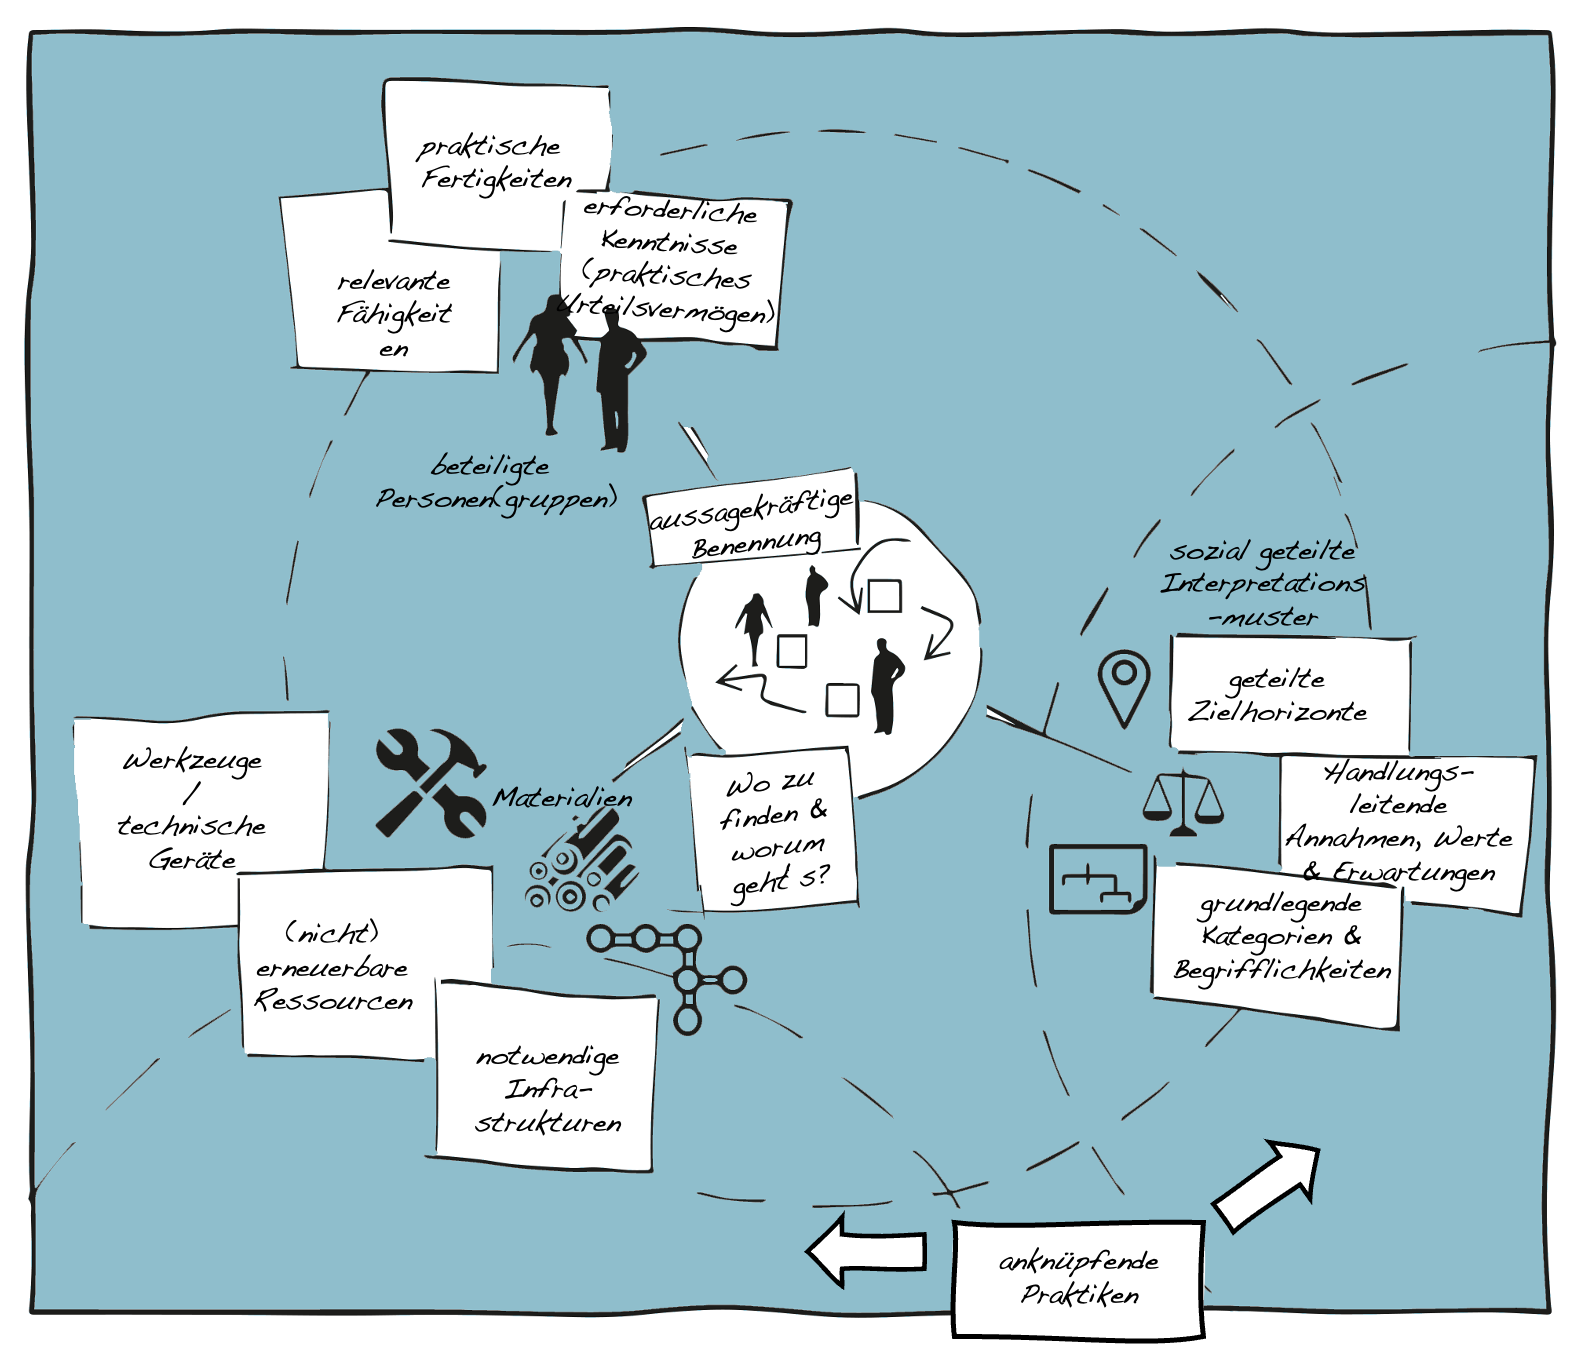
\includegraphics{Figures/05-03-Kartierung} \end{center}

\textbf{Arbeitsschritte}

\begin{enumerate}
\def\labelenumi{\arabic{enumi}.}
\tightlist
\item
  Auswahl und aussagekräftige Benennung der zu kartierenden Praktik.
\item
  ›Verortung‹ der Praktik: In welchem Kontext findet sie statt? Wer ist beteiligt? Worum geht es?
\item
  Beschreibung und ggf. Illustration wesentlicher Strukturelemente.
\item
  Kartierung angrenzender Praktiken, an denen dieselben Personen(gruppen), Materialien oder Interpretationsmuster beteiligt sind.
\item
  Ggf. Überarbeitung oder Erweiterung der Karte.
\end{enumerate}

\textbf{Ergebnisformat}

Eine grafische evtl. mit Bildern oder Verweisen angereichte Darstellung der wesentlichen Strukturelemente.

\textbf{Praktische Tipps}

\begin{itemize}
\tightlist
\item
  Die Karte sollte Außenstehenden eine Idee vom Sinn und Zweck der Praktik vermitteln und es ihnen ermöglichen, die Praktik zu erkennen, wenn sie ihr begegnen.
\item
  Die Beschreibung sollte sich an den Begrifflichkeiten der Praktiker*innen orientieren.
\end{itemize}

\textbf{»Fallstricke«}

\begin{itemize}
\tightlist
\item
  Soziale Praktiken sind keine fixen Einheiten. Die Strukturelemente können sich im Laufe der Zeit stark verändern. Ebenso kann es unterschiedliche ›Spielarten‹ ein und derselben Praktik gegeben. Die Kartierung sollte sich deshalb an den konkreten analytischen Interessen orientieren.
\item
  Viele Praktiken sind zwar eng mit bestimmten Technologien verknüpft. Der Einsatz einer Technik ist aber nie Selbstzweck. Insofern genügt der Verweis auf eine bestimmte Technologie nie aus, um eine Praktik zu charakterisieren.
\end{itemize}

\textbf{Weiterführende Literatur zum Leittext}

Schatzki, T. R. (2012). A primer on practices: Theory and research. In J. Higgs, R. Barnett, S. Billett, M. Hutchings, \& F. Trede (Hrsg.), Practice-based education (S. 13--26). New York: Sense Publisher.

Shove, E., Pantzar, M., \& Watson, M. (2012). The Dynamics of Social Practice---Everyday Life and how it Changes. Los Angeles: Sage.

\chapter{Technikgenese}\label{technikgenese}

Die Entwicklung und der Gebrauch technischer Dinge ist ein kultur- und epochenübergreifendes Phänomen. Dementsprechend haben auch die technischen Dinge, mit denen wir es heute zu tun haben, bereits eine mehr oder weniger lange und abwechslungsreiche Entwicklungsgeschichte hinter sich. Die Entwicklung und Verbreitung bestimmter Technologien ist dabei eng mit der Transformation sozialer Praktiken verknüpft. Der Buchdruck, das Auto wie auch der Computer sind hierfür nur einige sehr augenfällige Beispiele.

Das Konzept der Technikgenese bezieht sich auf die Prozesse der Entstehung, Entwicklung und Gestaltung von Technik. Je nach Erkenntnisinteresse nehmen technikgenetische Untersuchungen dabei zum Beispiel die Entwicklung einzelner technischer Produkte, die Entwicklungslinien einer Technologie oder auch die Gesamtheit technischer Entwicklungen innerhalb einer Epoche und Kultur in den Blick \citep{rammertTechnik2010}.

\begin{figure}
\centering
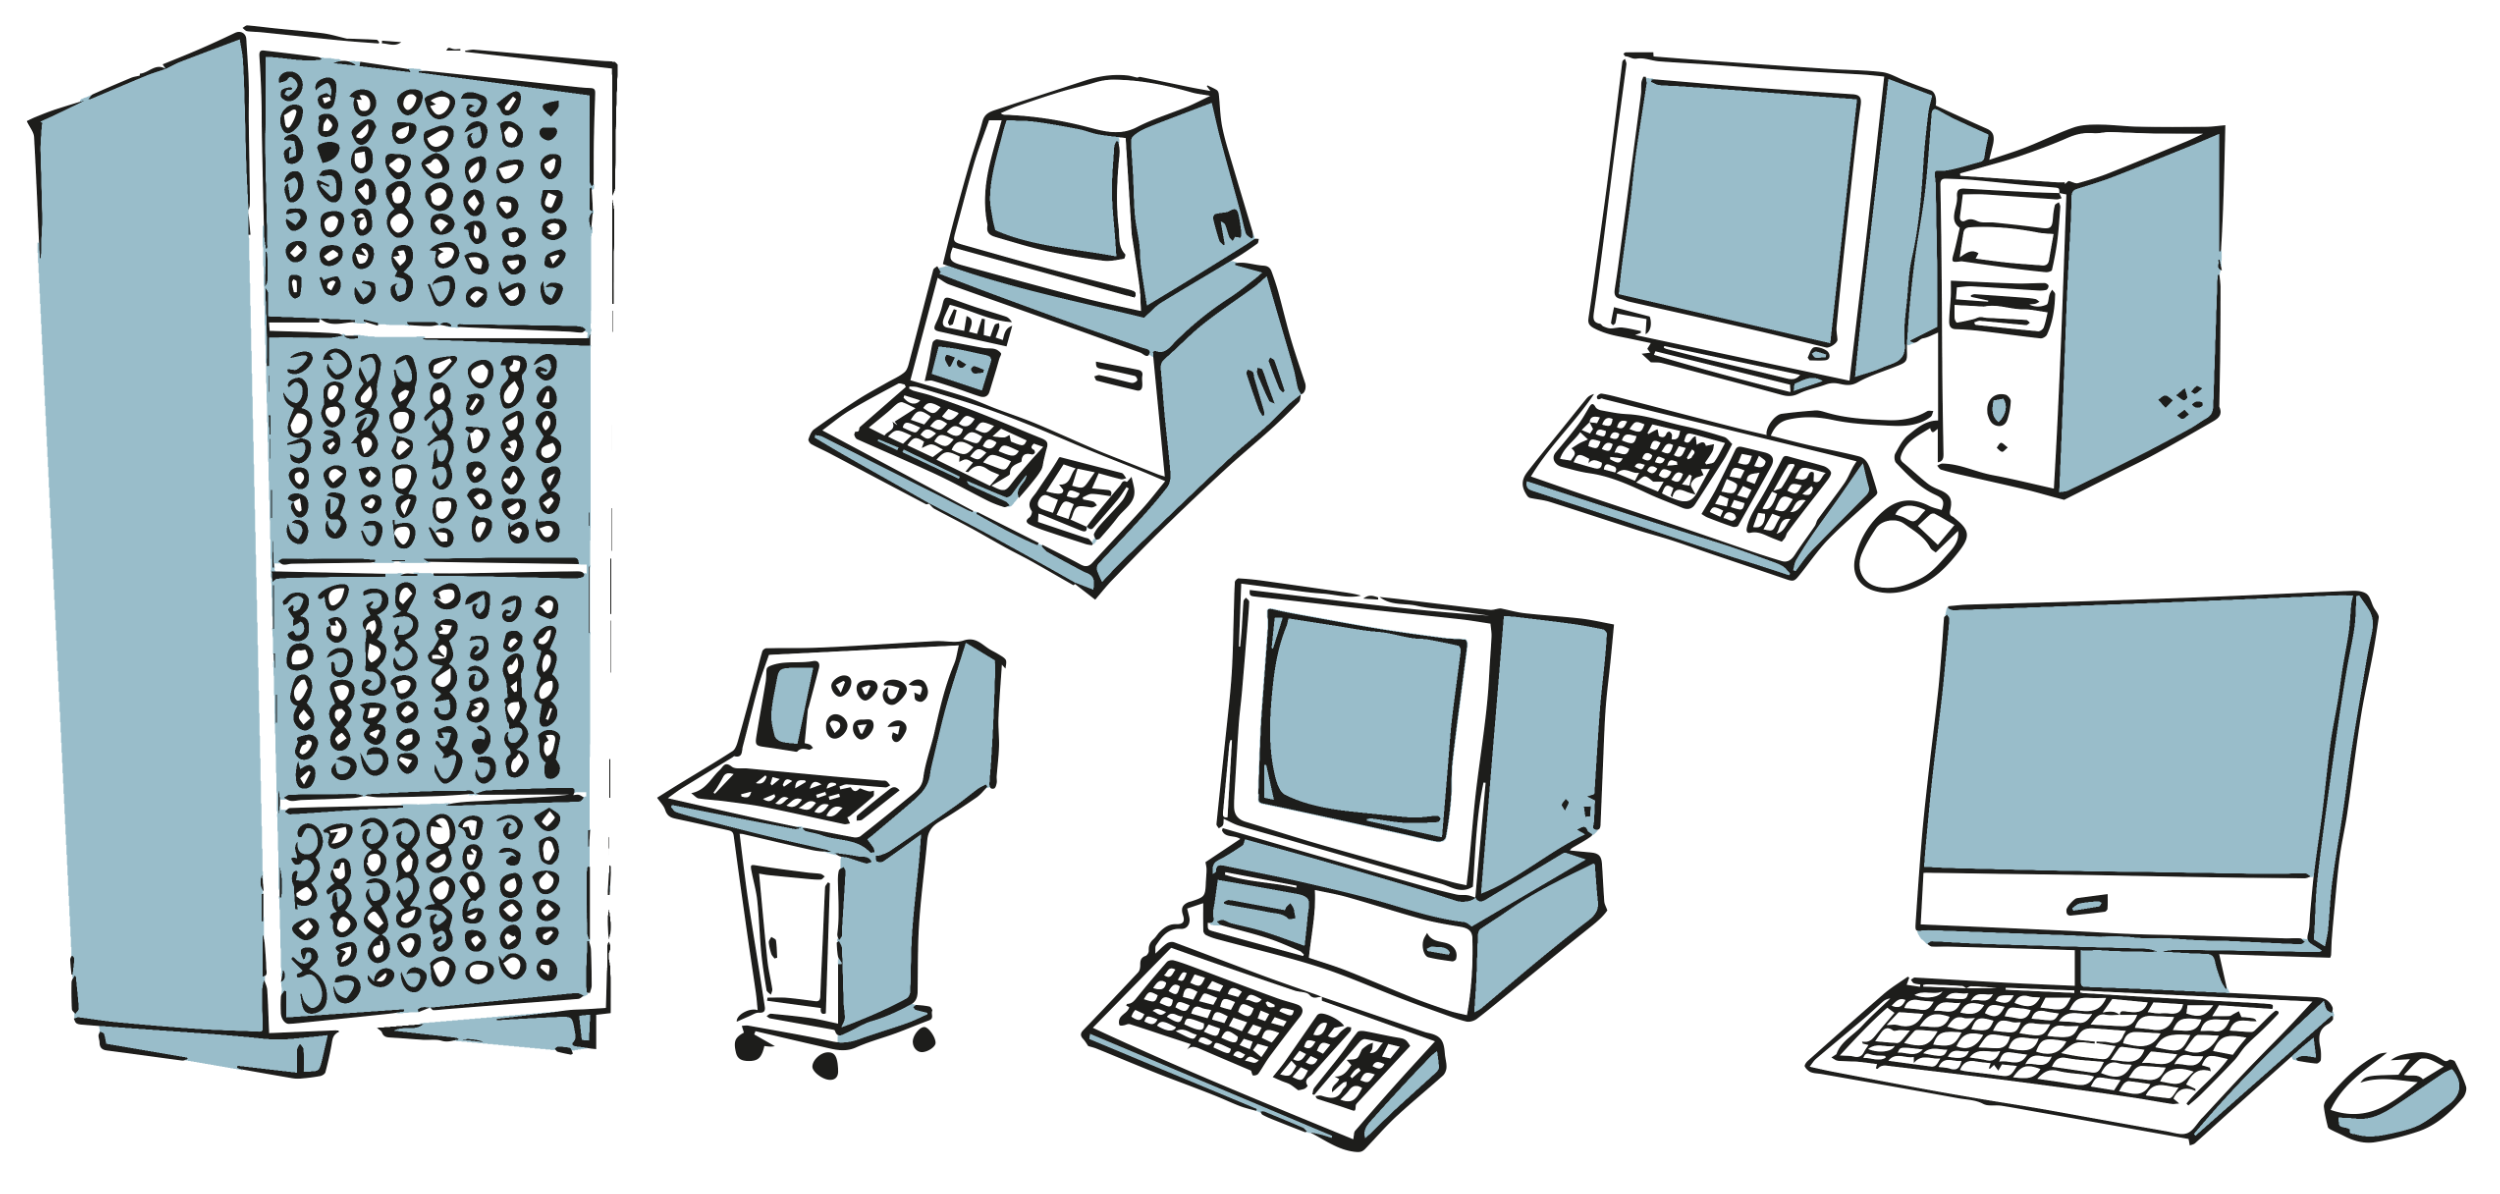
\includegraphics{Figures/06-01-Computer.png}
\caption{\label{fig:fig3}Der Computer im Wandel der Zeit (Illustration basierend auf einer Grafik von \href{https://www.freepik.com/free-vector/computers-evolution-cartoon-vector-concept-vintage-old-computing-stations-retro-system-units-monitors-modern-desktop-pc-with-keyboard-mouse-illustrations-set-isolated-white-background_4393734.htm\#query=computer\%20evolution&position=1&from_view=search&track=robertav1_2_sidr}{Freepik.com}).}
\end{figure}

\section{Konzepte der Technikgenese (1)}\label{konzepte-der-technikgenese-1}

Während in der sozial- und kulturwissenschaftlichen Diskussion die Vorstellung weit verbreitet ist, dass sich die \textbf{Entwicklung und der Gebrauch technischer Dinge als kulturell und historisch gerahmte Prozesse} verstehen lassen, besteht weniger Einigkeit hinsichtlich der Frage, wie sich entsprechende Prozesse analytisch fassen lassen. Je nach gewähltem analytischem Zugang verändert sich der Fokus und andere Aspekte treten in den Vordergrund. Das Spektrum technikgenetischer Perspektiven reicht hierbei von Ansätzen, die die Entwicklung technischer Dinge (a) als eine \textbf{Form intentionalen Handelns}, (b) als \textbf{soziale Aushandlungsprozesse} oder (c) als \textbf{koevolutionäre Transformationsprozesse} begreifen, in denen sich technische Dinge und soziale Praktiken gegenseitig bedingen und kontinuierlich verändern \citep[vgl.][]{fengThinkingDesignCritical2008, shoveDynamicsSocialPractice2012}.

\textbf{Technikgenese als intentionaler Prozess}

Modelle, die die Entstehung von Technik als einen intentionalen Prozess verstehen, betonen die Rolle derjenigen, die z.B. als Ingenieure, Designer*innen oder Softwareentwickler*innen unmittelbar an der Konzeption und Gestaltung der technischen Dinge beteiligt sind. Diese Modelle gehen davon aus, dass die für die konkreten Gestaltungsentscheidungen verantwortlichen Personen ein hohes Maß an Kontrolle über den Gestaltungsprozess wie auch die Produkte haben. Es sind aus dieser Perspektive die Entwickler*innen selbst, die aufgrund ihrer Rolle und ihres Know-Hows den Dingen eine Funktion und Bedeutung geben.

Intentionale Modelle widersetzen sich der Vorstellung technischen Fortschritts als einer inneren Notwendigkeit und betonen stattdessen die Rolle menschlicher Akteur*innen für die Entstehung technischer Dinge. Entsprechende Modelle finden sich insbesondere in den Design- und Ingenieurswissenschaften wieder, da sie einen wichtigen handlungspraktischen Rahmen für die an den entsprechenden Gestaltungsprozessen beteiligten Akteur*innen bieten \citep{carvalhoLegitimatingDesignSociology2009}. Die Betonung der intentionalen Seite der Technikgenese blendet aber die soziale und kulturelle Bedingtheit entsprechender Entwicklungen wie auch die Möglichkeiten nicht intendierter (Neben-)Wirkungen weitgehend aus \citep{ihdeDesignerFallacyTechnological2008}.

\section{Konzepte der Technikgenese (2)}\label{konzepte-der-technikgenese-2}

\textbf{Technikgenese als sozialer Aushandlungsprozess}

Im Unterschied zu intentionalen Modellen erweitert eine zweite Gruppe technikgenetischer Ansätze den Fokus und schließt die sozialen Rahmenbedingungen und Handlungskontexte mit ein, in denen technische Dinge konzipiert, hergestellt und implementiert werden. Technikgenese ist aus dieser Perspektive in Form sozialer Projekte organisiert, in denen unterschiedliche Interessengruppen über technische Optionen verhandeln und entscheiden welche Technik letztlich realisiert wird \citep[vgl. z.B.][]{woodhouseDesignSocietyScience2004}. Dementsprechend sind es vor allem die sozialen und politischen Entstehungszusammenhänge, die die Funktionalität und Bedeutung der technischen Artefakte bestimmen.

Die Vorstellung der Technikgenese als einem sozialen Aushandlungsprozess relativiert den Einfluss der Entwickler*innen und ihrer Intentionen und betont stattdessen die Bedeutung ökonomischer, politischer, institutioneller, sozialer und kultureller Faktoren für technische Entwicklungsvorhaben. Die Technikgenese wird damit zu einem macht- und interessengeladenen Prozess \citep[vgl.][]{fengThinkingDesignCritical2008}. Ähnlich wie die intentionalen Modelle gehen auch diese Ansätze davon aus, dass die Form, Funktion und Bedeutung technischer Dinge maßgeblich durch den jeweiligen Entstehungszusammenhang bestimmt wird, während sowohl dem Gebrauch wie auch den materiellen Eigenschaften der Dinge nur eine untergeordnete Bedeutung beigemessen wird. Zugespitzt formuliert erscheinen die technischen Dinge aus dieser Perspektive als eine ›geronnene‹ und auf Dauer gestellte Form sozialer Praxis \citep{mackenzieProblematisingTechnologicalObject2005}.

\textbf{Technikgenese als koevolutionärer Transformationsprozess}

Eine dritte Gruppe von Ansätzen setzt schließlich die Entwicklung und den praktischen Gebrauch technischer Dinge miteinander in Beziehung und geht davon aus, dass diese Prozesse miteinander verschränkt sind. Die Funktionalität und Bedeutung ist aus dieser Perspektive den technischen Dingen nicht ›eingeschrieben‹, sondern muss im praktischen Gebrauch immer wieder neu reproduziert werden. Die Entwicklung technischer Dinge knüpft in diesen Modellen immer schon an die bereits bestehenden Praktiken und vorhandenen technischen Gegebenheiten an und ist insofern eingebettet in entsprechende soziale und technische Milieus.

Koevolutionäre Modelle betonen die Prozess- und Ereignishaftigkeit technischer Entwicklungen \citep{mackenzieProblematisingTechnologicalObject2005}. Sie heben insbesondere die praktischen Leistungen der Anwender*innen hervor, die notwendig sind, um die Funktion und Bedeutung der Dinge im praktischen Gebrauch sicherzustellen und »die Technik ›am Laufen {[}zu{]} halten‹« \citep{horningExpertenAlltags2001}. Zudem unterlaufen sie die Vorstellung einer umfassenden Veränder- und Formbarkeit der Technik, indem sie individuelle Entwicklungsvorhaben mit vorausgegangenen technologischen Entwicklungslinien in Beziehung setzen \citep[z.B.][]{lawsonOntologyTechnologyArtefacts2008, riederEnginesOrderMechanology2020}.

\begin{blackbox}
\emph{Wie haben sich etwa die Praktiken des Schreibens und Zeichnens mit der Erfindung von Bleistift und Radiergummi verändert \citep[siehe hierzu ausführlicher etwa][]{oelkersHistorizitatPadagogischerGegenstande2012}?}

\end{blackbox}

~

\begin{center}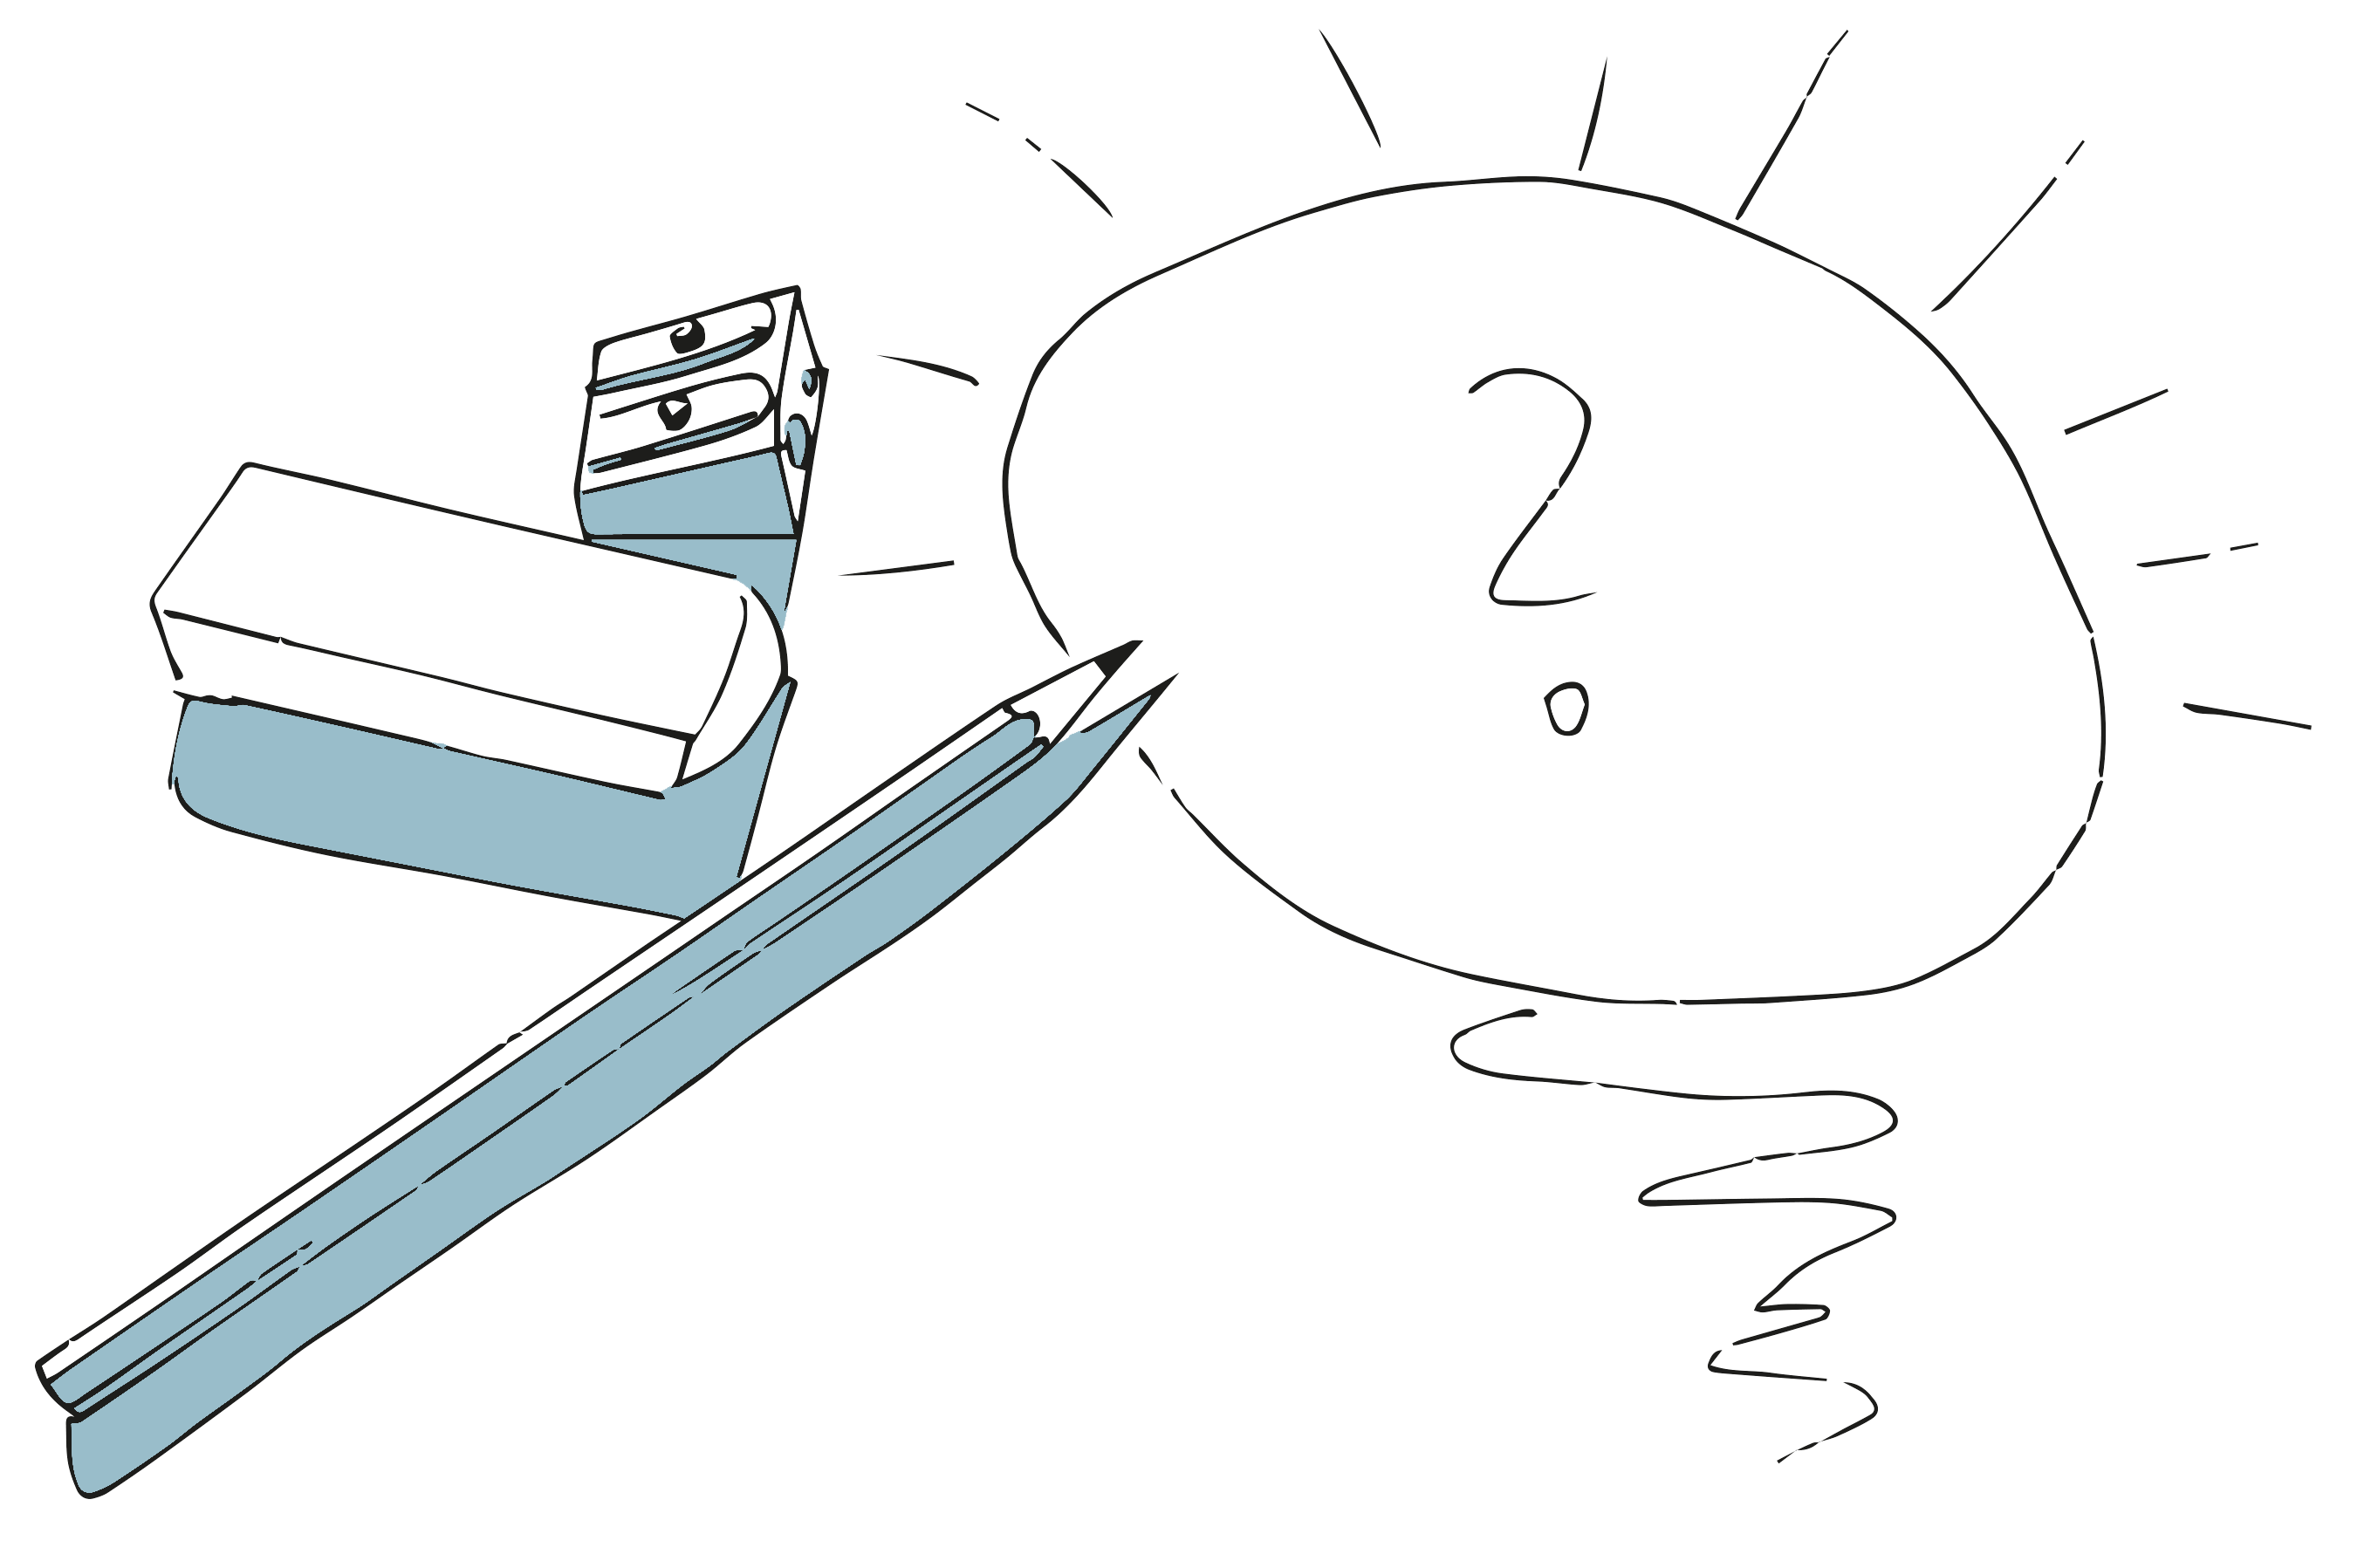
\includegraphics{Figures/06-02-Pencil} \end{center}

\section{Qualitative Gegenüberstellungen}\label{qualitative-gegenuxfcberstellungen}

\textbf{Ziel}

Qualitative Gegenüberstellungen dienen dazu, Gemeinsamkeiten und Unterschiede zwischen zwei oder mehr Untersuchungsgegenstände/Fällen zu identifizieren.

\textbf{Leitgedanke}

Ein systematischer Vergleich von Gegenständen/Fällen setzt die Kenntnis von Merkmalsdimensionen voraus, die für den jeweiligen Untersuchungszusammenhang relevant sind und anhand derer sich Gemeinsamkeiten und Unterschiede festmachen lassen. In vielen Fällen sind diese Merkmalsdimensionen zu Beginn der Untersuchung aber noch nicht vollständig bekannt, sodass diese anhand des Datenmaterials sukzessive (weiter-)entwickelt werden müssen. Die qualitative Gegenüberstellung dient insofern nicht nur dazu, Gegenstände/Fälle anhand vorhandener Kriterien zu beschreiben, sondern auch herauszufinden, worin relevante Unterschiede überhaupt bestehen könnten.

\textbf{Anwendungskontext}

Qualitative Gegenüberstellungen bieten sich insbesondere dann an, wenn die zu vergleichenden Gegenständen/Fälle komplexer Art sind und/oder die relevanten Vergleichsdimensionen noch unbekannt sind.

\begin{center}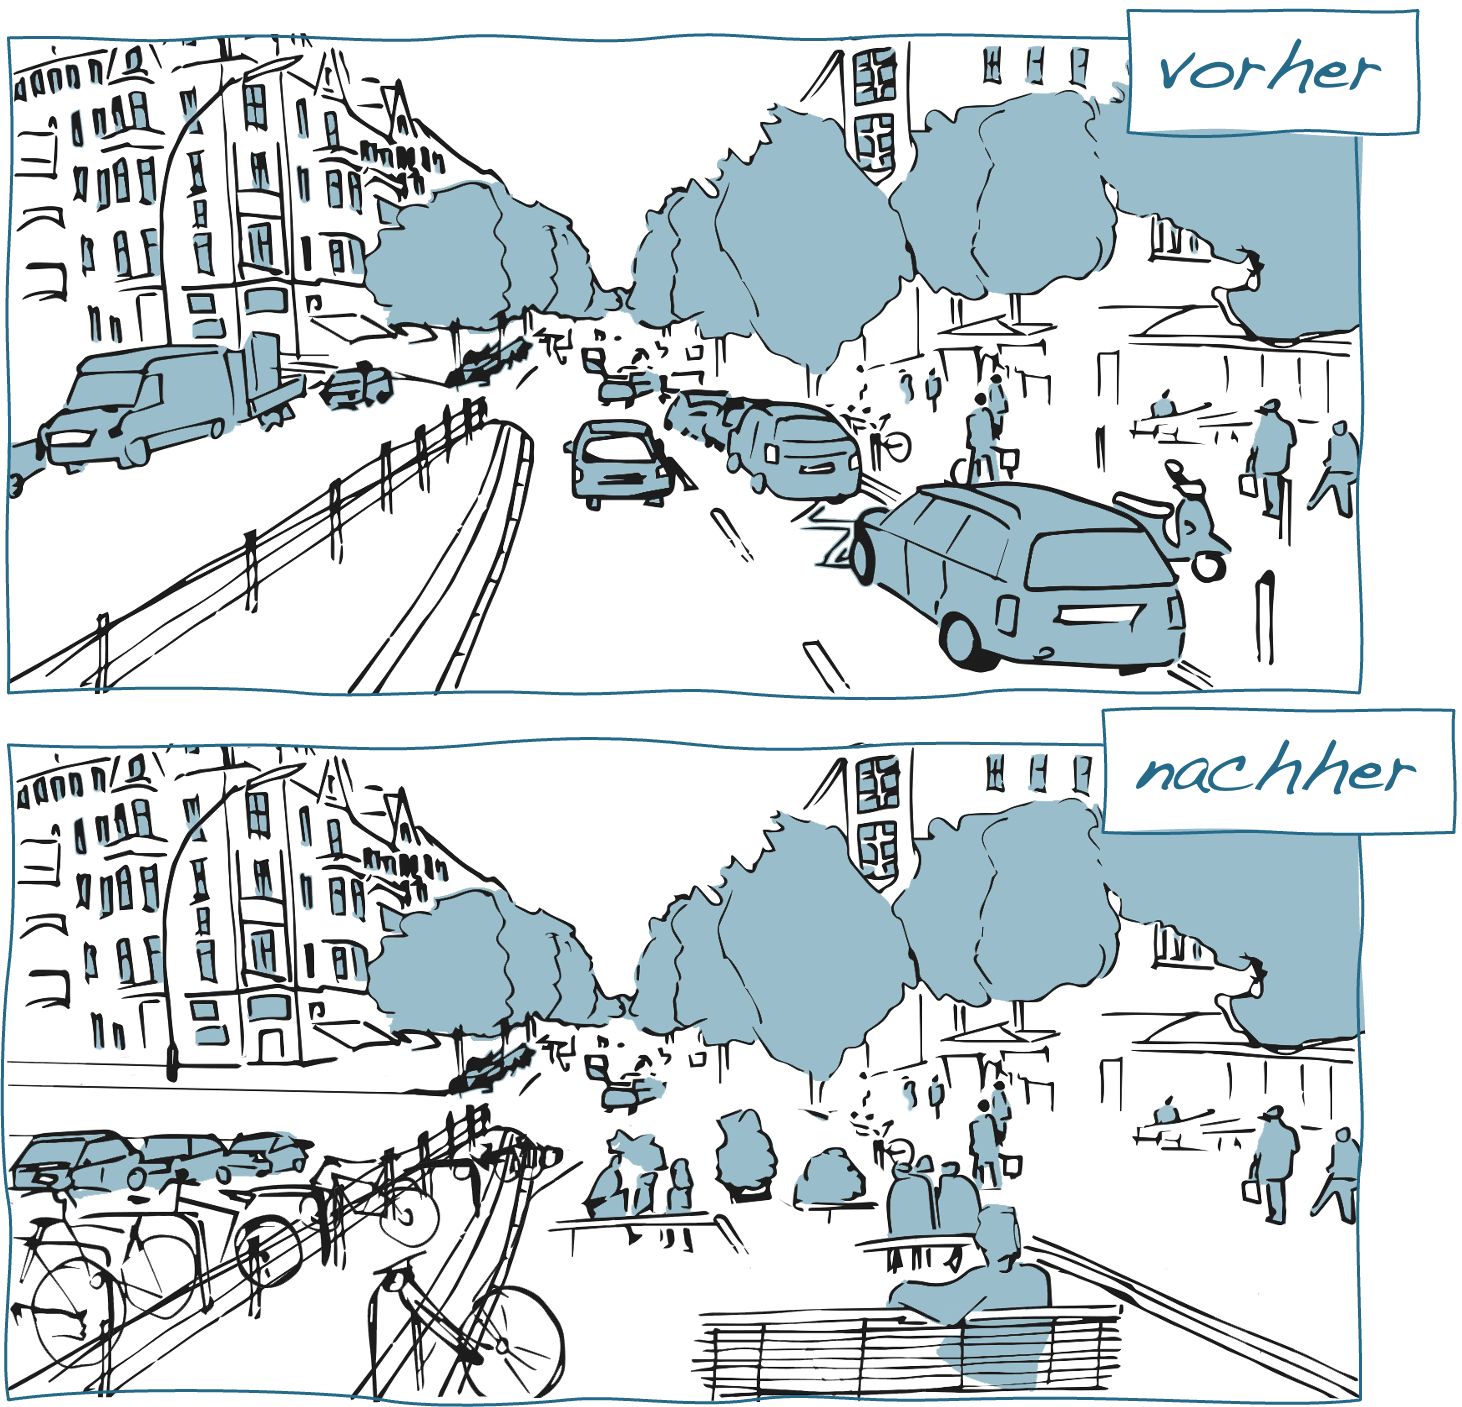
\includegraphics{Figures/06-03-vorher-nachher} \end{center}

\textbf{Arbeitsschritte}

\begin{enumerate}
\def\labelenumi{\arabic{enumi}.}
\tightlist
\item
  Auswahl der zu vergleichenden Untersuchungsgegenstände/Fälle.
\item
  Vorläufige Festlegung relevanter Vergleichsdimensionen.
\item
  Sammlung von Informationen und Beschreibung der Gegenstände/Fälle unter Berücksichtigung der Vergleichsdimensionen.
\item
  Falls erforderlich, Überarbeitung oder Erweiterung der Vergleichsdimensionen.
\item
  Dokumentation der zentralen Gemeinsamkeiten und Differenzen.
\end{enumerate}

\textbf{Ergebnisformat}

Eine grafische oder tabellarische Aufstellung der identifizierten Gemeinsamkeiten und Unterschiede.

\textbf{Praktische Tipps}

\begin{itemize}
\tightlist
\item
  Bei der Auswahl der Vergleichsdimensionen ist darauf zu achten, dass diese inhaltlich wirklich relevant sind. Aus diesem Grund sollten auch die Ergebnisse der Gegenüberstellung mit dem bereits vorhandenen (Vor-)Wissen abgeglichen werden.
\item
  Neben quantitativen Differenzen sollte bei der Gegenstellung insbesondere auf qualitative Unterschiede geachtet werden, die z.B. die Funktionsweise, Struktur oder Bedeutung der Gegenstände/Fälle betreffen.
\end{itemize}

\textbf{»Fallstricke«}

\begin{itemize}
\tightlist
\item
  Qualitative Gegenüberstellungen sind kein linearer Prozess, sondern erfordern die wiederholte Reflexion der zugrunde gelegten Vergleichsdimensionen.
\end{itemize}

\textbf{Weiterführende Literatur zum Leittext}

Adamson, B. (2019). Juxtaposing Comparative Education and Teacher Education. In M. A. Peters (Hrsg.), \emph{Encyclopedia of Teacher Education} (S. 899-904). Springer Singapore.

Miles, M. B., \& Huberman, A. M. (1994). \emph{Qualitative Data Analysis} (2nd. ed.). Sage.

\chapter{Transformation sozialer Praktiken}\label{transformation-sozialer-praktiken}

Vertreter*innen der praxistheoretischer Positionen betonen die konstitutive Verwicklung von Mensch und Technik, von Technologien und sozialen Praktiken \citep{horningExpertenAlltags2001, orlikowskiUsingTechnologyConstituting2000, schatzkiMaterialitySocialLife2010, shoveDynamicsSocialPractice2012}. Sie folgen damit im Wesentlichen der Idee der Technikgenese als einem koevolutionären Transformationsprozess, innerhalb dessen sich soziale Praktiken und technische Dinge gegenseitig bedingen und kontinuierlich transformieren. Um die hiermit einhergehenden Vorgänge fassen zu können, haben Elisabeth Shove, Mika Pantzar \& Matt Watson \citep{shoveDynamicsSocialPractice2012} ein Modell vorgeschlagen, mit dem sich die dynamische Veränderung sozialer Praktiken beschreiben und analysieren lässt.

Das Modell basiert auf einer bewussten Vereinfachung praxistheoretischer Grundannahmen und Konzepte, bietet damit aber zugleich die Möglichkeit Transformationsprozesse auf unterschiedlichen Abstraktionsebenen zu analysieren. Für eine weiterführende Übersicht über praxistheoretische Grundkonzepte siehe zum Beispiel Theodore Schatzki \citep{schatzkiPrimerPracticesTheory2012}.

\section{Materielle Dinge, praktische Kompetenzen \& soziale Bedeutungen}\label{materielle-dinge-praktische-kompetenzen-soziale-bedeutungen}

Shove, Pantzar und Watson \citep{shoveDynamicsSocialPractice2012} gehen in ihrem Modell davon aus, dass sich soziale Praktiken im Zusammenspiel \textbf{materieller Dinge} (materials), praktischer Kompetenzen (competences) und sozialer Bedeutungen (meanings) ausbilden und (weiter-)entwickeln.

Die materiellen Dinge umfassen dabei das gesamte Spektrum an Gegenständen, Werkzeugen, Geräten und Instrumenten, die in einer Praktik zum Einsatz kommen, wie auch die materiellen Ressourcen und Infrastrukturen, die für die Durchführung einer Praktik notwendig sind oder in ihr verarbeitet werden. Zu den materiellen Dingen gehören auch die Körper derjenigen, die aktiv oder passiv an einer Praktik beteiligt sind. Technische Dinge, wie etwa ein Fahrrad, ein Smartphone, ein WLAN aber auch ein digitales Textdokument sind aus dieser Perspektive ein Teil jener materiellen Dinge, die in bestimmten sozialen Praktiken Verwendung finden.

Zu den \textbf{praktischen Kompetenzen} zählen hier all jene Fähigkeiten und Fertigkeiten, die zur aktiven Teilhabe an einer bestimmten sozialen Praktik erforderlich sind, sowie die entsprechenden Kenntnisse. Zu diesen Kenntnissen gehört insbesondere ein allgemeines Verständnis für die mit der jeweiligen Praktik verbundenen Regeln, Werte und Normen, wie auch das Wissen über die Funktion und das Zusammenspiel der einzelnen Elemente. Die Kompetenzen umfassen ebenfalls ein auf die jeweilige Praktik bezogenes Urteilsvermögen, dass es den Praktiker*innen zum Beispiel erlaubt, eine Handlung als Teil einer Praktik zu erkennen oder auch die Qualität der Ausführung zu beurteilen. Bezogen auf den Umgang mit den technischen Dingen beinhalten die praktischen Kompetenzen auch jenes ›Know-how‹, das für den adäquaten Umgang mit den Dingen erforderlich ist. Der Umgang umfasst dabei neben dem direkten Gebrauch zum Beispiel Fragen der Anschaffung und Auswahl von Geräten wie auch deren Instandhaltung, Pflege und Reparatur.

Das dritte Element bilden schließlich die \textbf{sozialen Bedeutungen}, die mit einer sozialen Praktik verbunden sind und diese auszeichnen. Sie umfassen jene von den Praktiker*innen geteilten sozialen Interpretations- und Deutungsmuster, die für das Verständnis des gemeinsamen Miteinandertuns grundlegend und zielbestimmend sind. Hierzu zählen unter anderem geteilte Zielhorzionte, praxisleitende Annahmen, Werte und Erwartungen, wie auch grundlegende Kategorien und Begrifflichkeiten. In Hinblick auf die technische Dimension einer sozialen Praktik umfassen die sozialen Interpretations- und Deutungsmuster zum Beispiel die an den Einsatz einer bestimmten Technologie geknüpften Erwartungen und Werte wie auch hieraus resultierende Verantwortlichkeiten Formen der Arbeitsteilung.

Zusammengenommen bilden die materiellen Dinge, praktischen Kompetenzen und sozialen Bedeutungen das Grundgerüst einer sozialen Praktik. Shove, Pantzar und Watson stellen dieses Grundgerüst in Form einer dynamischen Dreiecksbeziehung dar (siehe {Abb. 7.1}).

\begin{figure}

{\centering 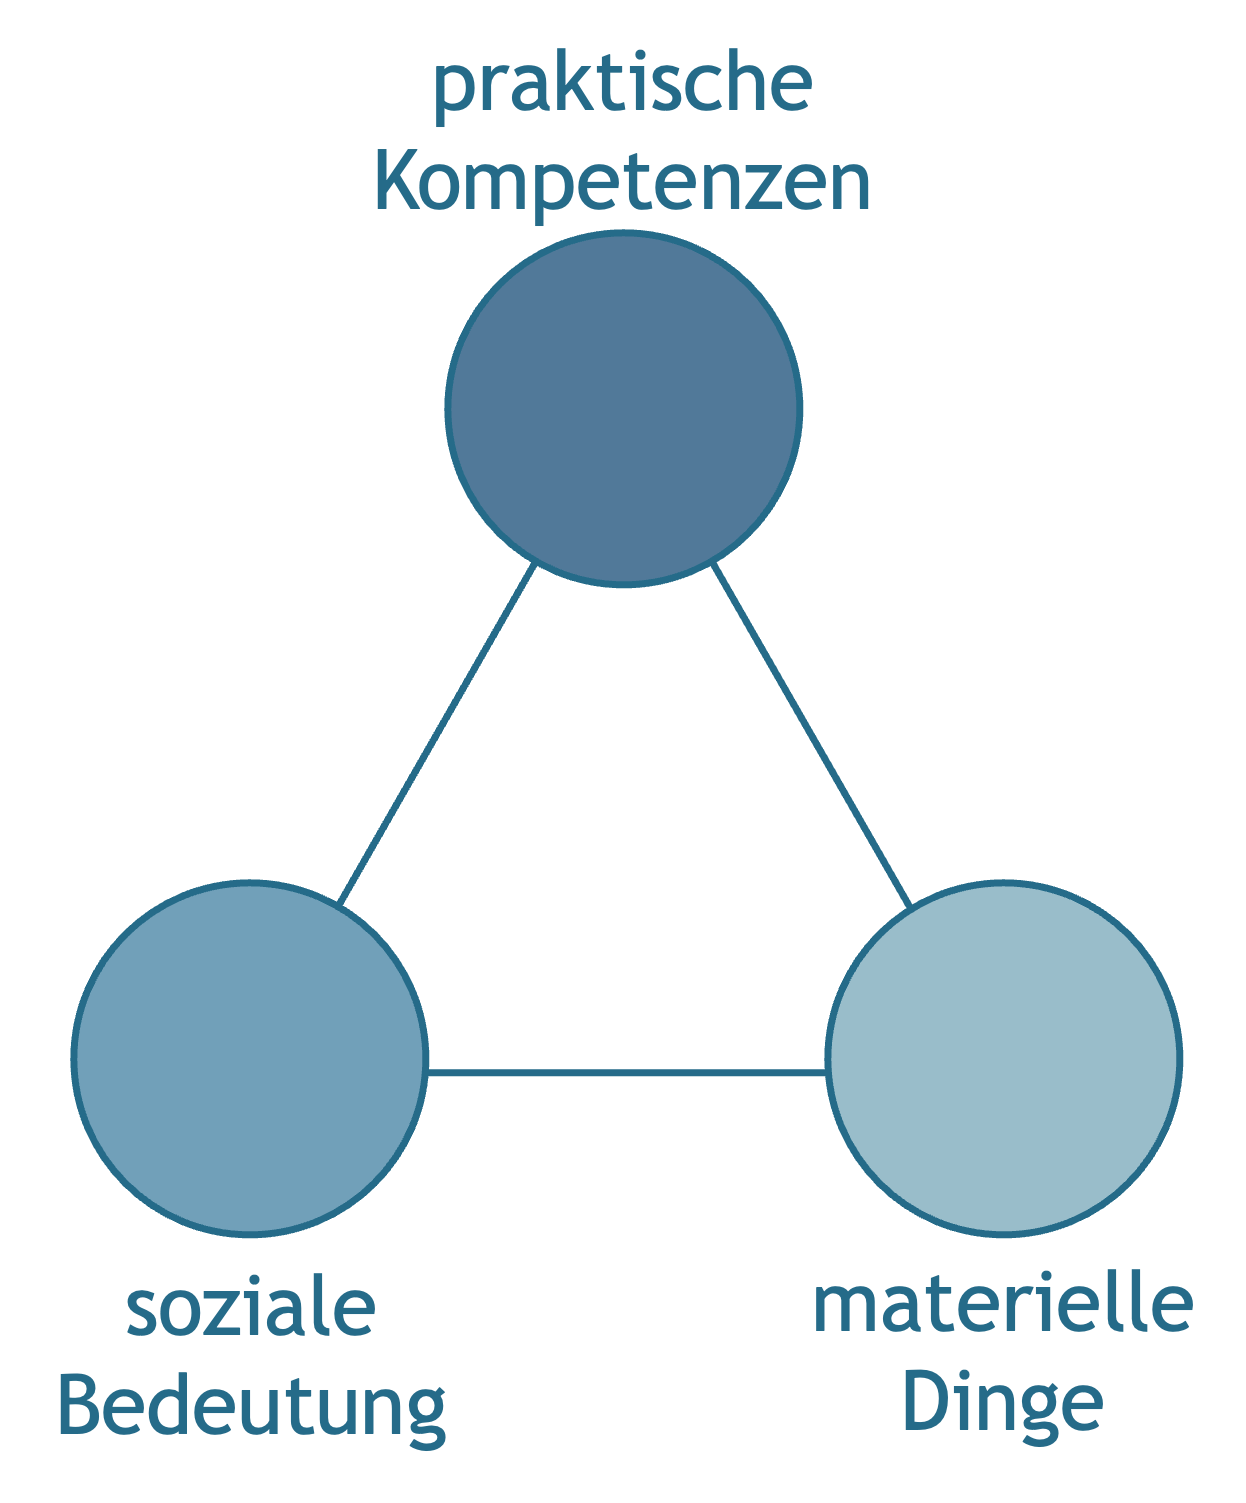
\includegraphics[width=0.5\linewidth]{Figures/07-01-Elemente-sozialer-Praktiken} 

}

\caption{Elemente sozialer Praktiken (in Anlehnung an Shove et al., 2012, S. 25).}\label{fig:fig4}
\end{figure}

\section{Soziale Praktiken -- Form \& Veränderung}\label{soziale-praktiken-form-veruxe4nderung}

Um der Veränderlichkeit sozialer Praktiken wie auch technischer Dinge Rechnung tragen zu können, schlagen Shove, Pantzar und Watson vor, die materiellen Dinge, praktischen Kompetenzen und sozialen Bedeutungen als mehr oder weniger eigenständige ›Elemente‹ zu verstehen, die aber zugleich im Rahmen sozialer Praktiken in grundlegender Weise aufeinander verweisen und aufeinander angewiesen sind.

Dieser gedankliche Spagat macht es möglich, die sukzessive Ausbildung von Dingen, Kompetenzen und Bedeutungen wie auch ihre Verschränkung im Rahmen sozialer Praktiken in den Blick zu nehmen und damit Abhängigkeiten und Transformationen auf unterschiedlichen Ebenen nachzuzeichnen. Materielle Dinge, wie ein Computer oder ein Fahrrad, können dementsprechend Teil unterschiedlicher Praktiken sein. Gleiches gilt auch für Kompetenzen und soziale Bedeutungen, die sich einerseits im Rahmen bestimmter Praktiken ausbilden aber zugleich auch in anderen Praktiken zum Tragen kommen können. Das Erlernen grundlegender Fertigkeiten, wie etwa des Lesens, Schreibens und Rechnens, aber auch grundlegende Wertorientierungen und allgemein anerkannte Wissensbestände sind typische Beispiele hierfür.

Vor diesem Hintergrund lassen sich drei grundlegende Transformationsdynamiken unterscheiden. Die \textbf{erste Transformationsdynamik} resultiert dabei aus den \textbf{Wechselbeziehungen der Elemente} innerhalb einer bestehenden Praktik. Da sich eine Praktik nicht in ihrer Wiederholung erschöpft, sind immer wieder Anpassungen und Veränderungen der einzelnen Elemente notwendig, um die Praktik ›am Laufen zu halten‹. Neue Praktiker*innen kommen hinzu und müssen die notwendigen Kompetenzen erwerben, technische Geräte nutzen sich ab und müssen ersetzt und repariert werden, Vorstellungen zum angemessenen Umgang miteinander aber auch mit den Dingen verändern sich. Veränderungen einzelner Elemente wirken sich dabei für gewöhnlich auch auf das Gesamtgefüge aus (vgl. {Abb. 7.2}).

\begin{figure}

{\centering 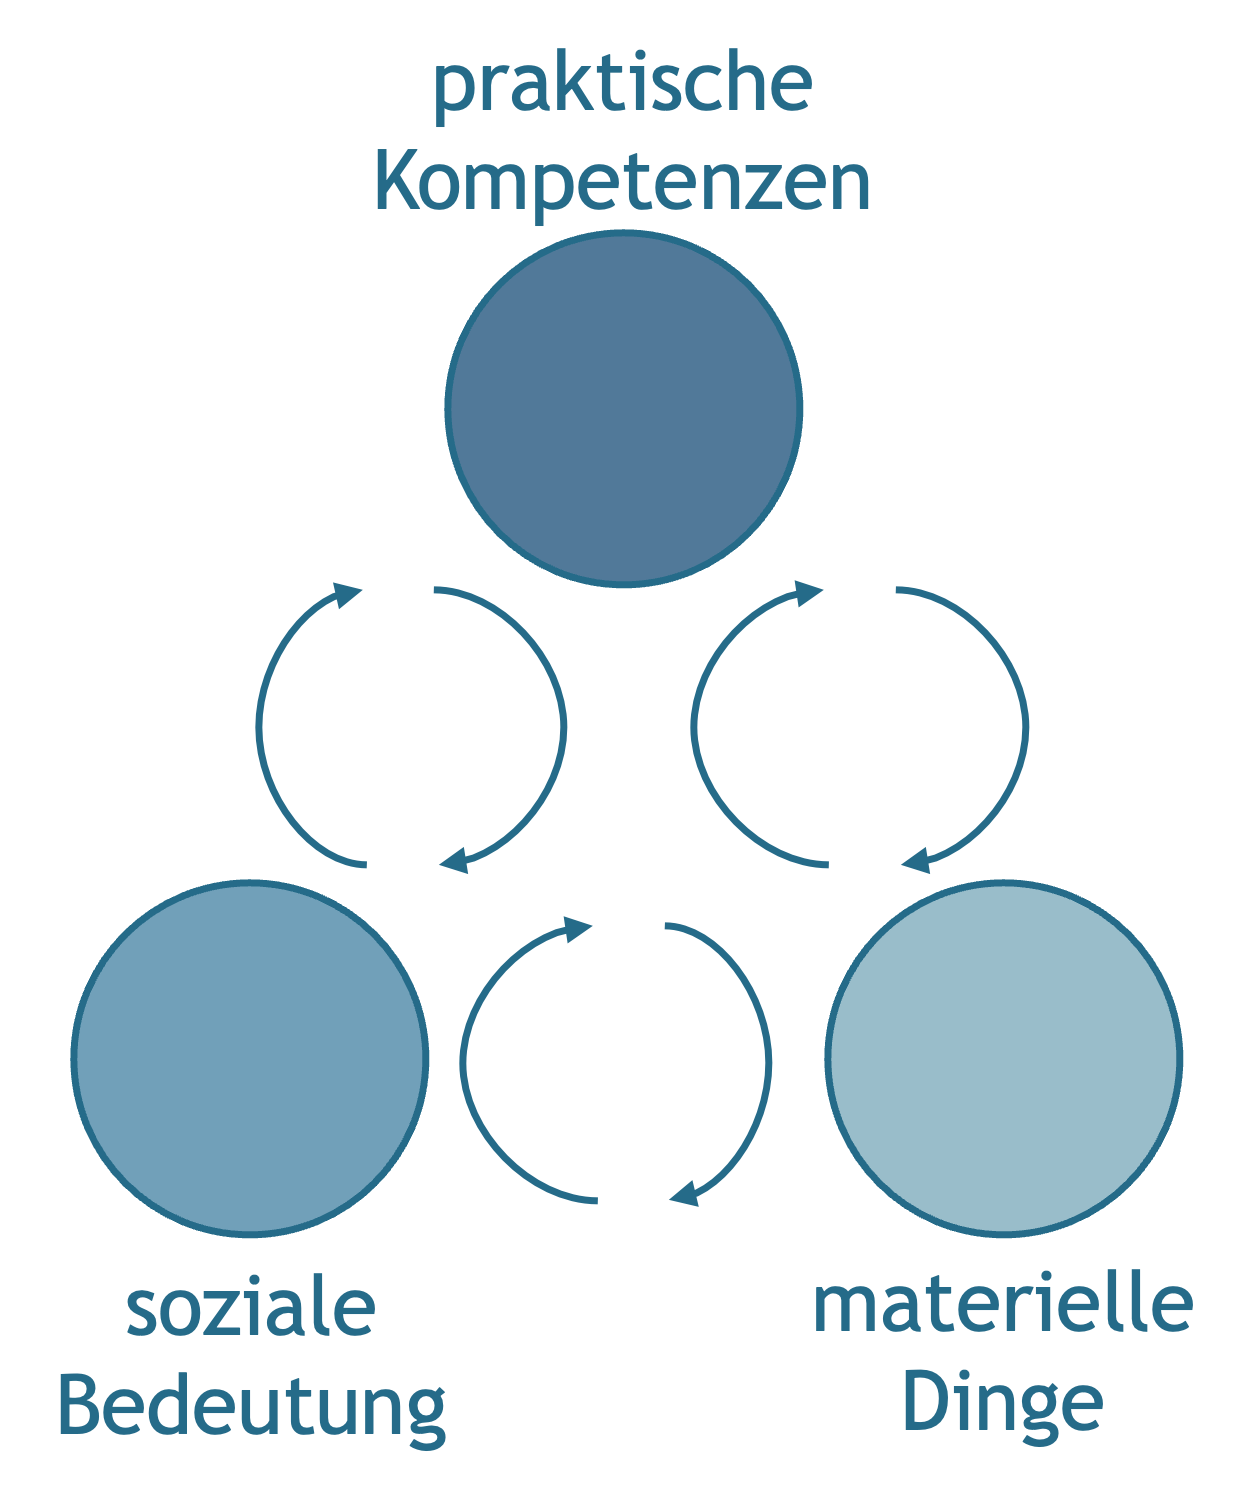
\includegraphics[width=0.5\linewidth]{Figures/07-02-Formung-Elemente} 

}

\caption{Die wechselseitige ›Formung‹ der Elemente einer Praktik (in Anlehnung an Shove et al., 2012, S. 32).}\label{fig:fig5}
\end{figure}

Die \textbf{zweite Transformationsdynamik} ergibt sich hingegen aus der \textbf{sukzessiven Veränderung einzelner Elemente} einer Praktik entlang eigener ›Entwicklungspfade‹ (vgl. {Abb. 7.3}). Technische Innovationen, die systematische Förderung allgemeiner Kompetenzen oder auch ein grundlegender Wertewandel, der über einzelne Praktiken hinausweist, können hierfür als Beispiele dienen.

\begin{figure}

{\centering 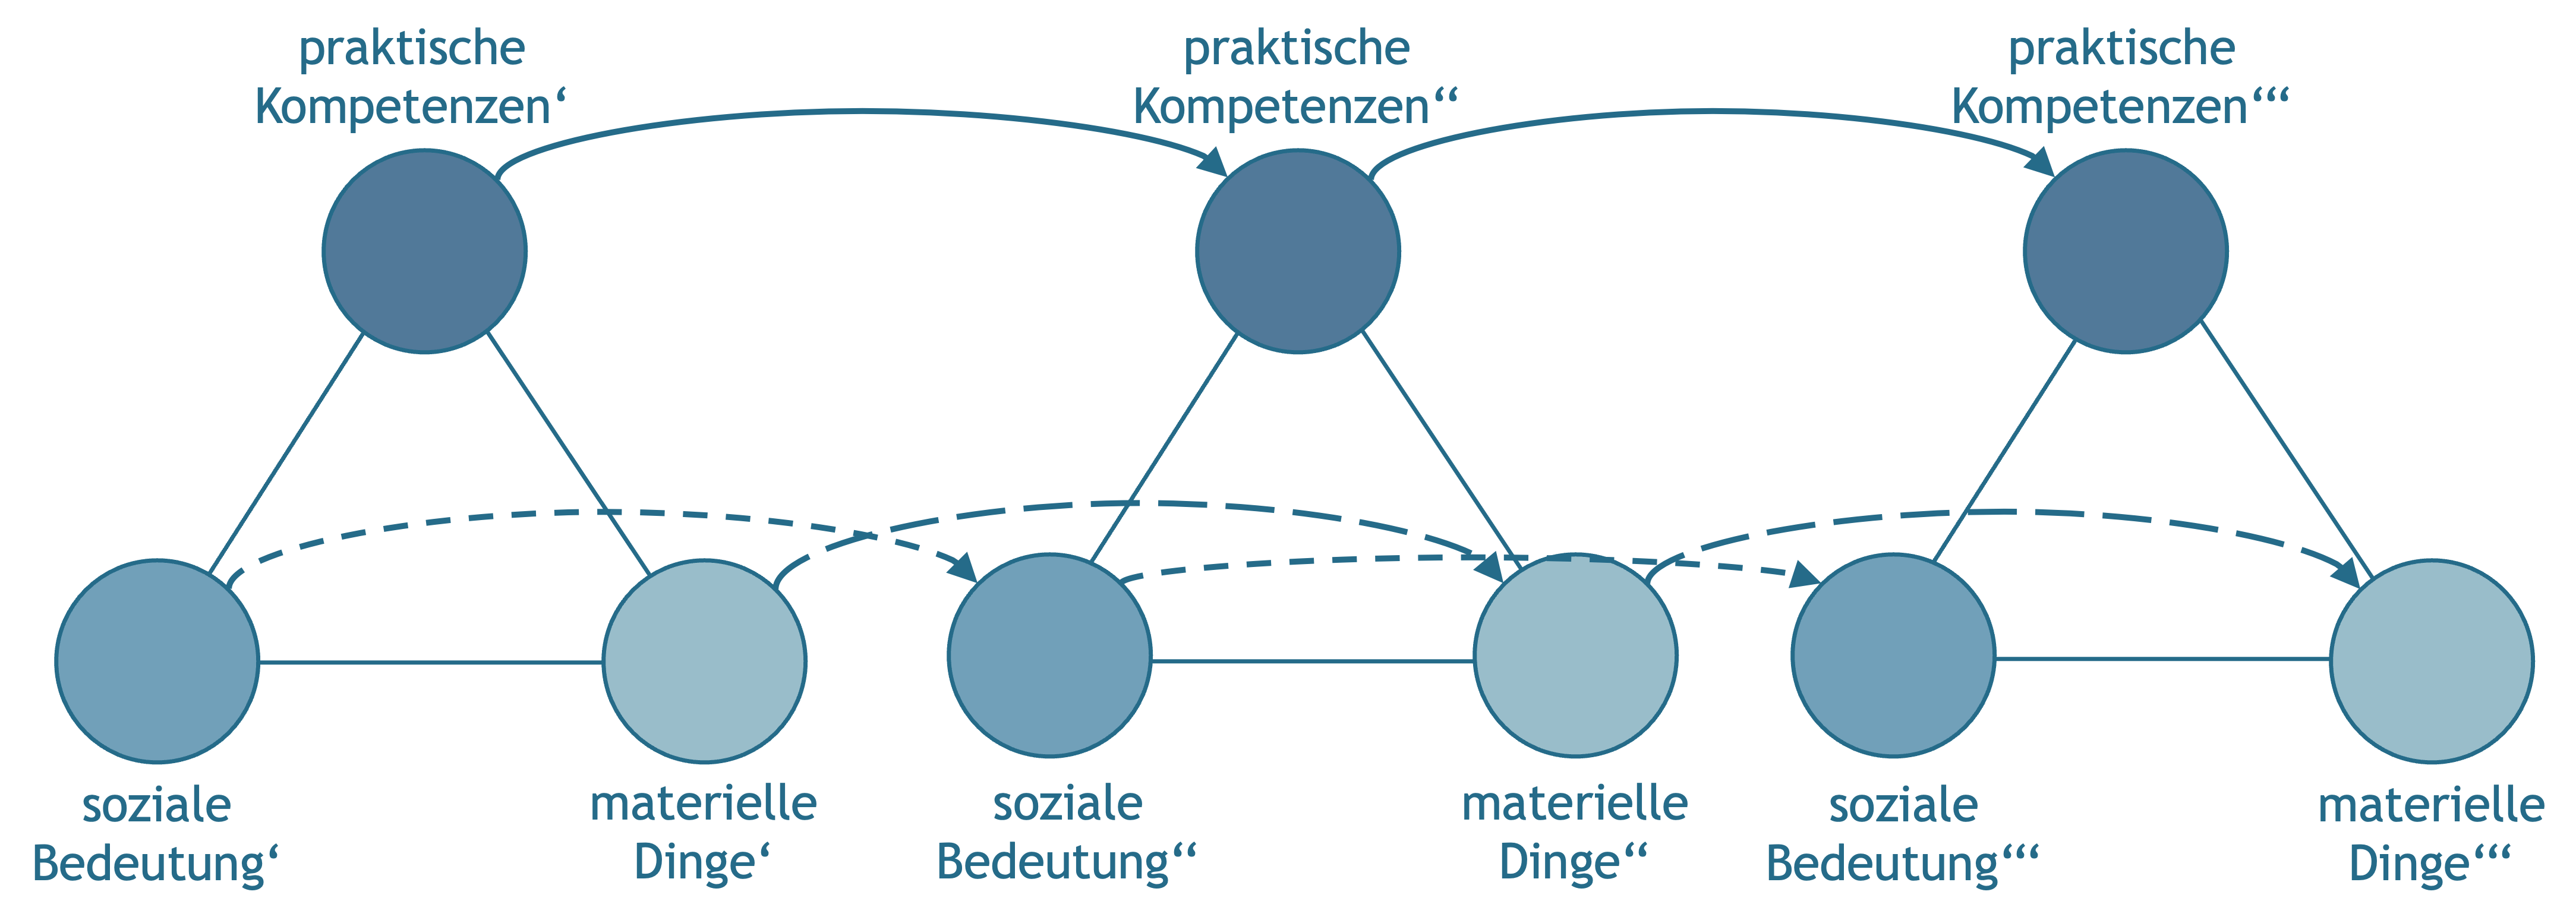
\includegraphics{Figures/07-03-Entwicklung-Elemente} 

}

\caption{Entwicklung der Elemente entlang eigener Pfade (in Anlehnung an Shove et al., 2012, S. 33).}\label{fig:fig6}
\end{figure}

Eine \textbf{dritte Transformationsdynamik} basiert schließlich auf der \textbf{Verknüpfung mehrerer Praktiken} durch die Bezugnahme auf ein gemeinsames Element. Veränderungen in einer Praktik können sich hierdurch auf andere Praktiken auswirken (vgl. {Abb. 7.4}). So kann beispielsweise ein Spielplatz seine Bedeutung für die Kinder einer Nachbarschaft verändern, wenn er zum Treffpunkt der Jugendlichen wird. Ebenso ändern sich beispielweise auch die Anforderungen an ein Auto, wenn dieses nicht nur als Transportmittel auf dem Weg zur Arbeit, sondern auch als Bastelobjekt, Statussymbol oder mobile Unterkunft im Urlaub dienen soll.

\begin{blackbox}
\emph{Anhand welcher Beispiele lassen sich die verschiedenen ›Transformationsdynamiken‹ veranschaulichen?}

\end{blackbox}

~

\begin{figure}

{\centering \includegraphics[width=0.75\linewidth]{Figures/07-04-Verknüpfung-Praktiken} 

}

\caption{Verknüpfung mehrerer Praktiken durch Bezugnahme auf ein gemeinsames Element (in Anlehnung an Shove et al., 2012, S. 37).}\label{fig:fig7}
\end{figure}

\section{Szenarien}\label{szenarien}

\textbf{Ziel}

Szenarien dienen der illustrativen Beschreibung prototypischer Handlungssequenzen in einem bestimmten Kontext.

\textbf{Leitgedanke}

Szenarien beschreiben einen typischen Handlungsverlauf. Sie sollen es ermöglichen, sich in eine Situation hineinzuversetzen und zu verstehen, welche Aspekte für eine Handlung relevant sind.
Im Rahmen eines Szenarios sollte deutlich werden: \textbf{wer} an der Handlung beteiligt ist, welche \textbf{Ziele} die Akteur*innen verfolgen, was sie \textbf{tun}, aber auch was sie \textbf{denken} und \textbf{fühlen}. Darüber hinaus sollte das Szenario über die \textbf{Kontextfaktoren} und \textbf{Ereignisse} informieren, die den Handlungsverlauf beeinflussen.

\textbf{Anwendungskontext}

Szenarien können sowohl zur zusammenfassenden Beschreibung aktueller wie auch fiktiver Handlungsabläufe verwendet werden.

\begin{center}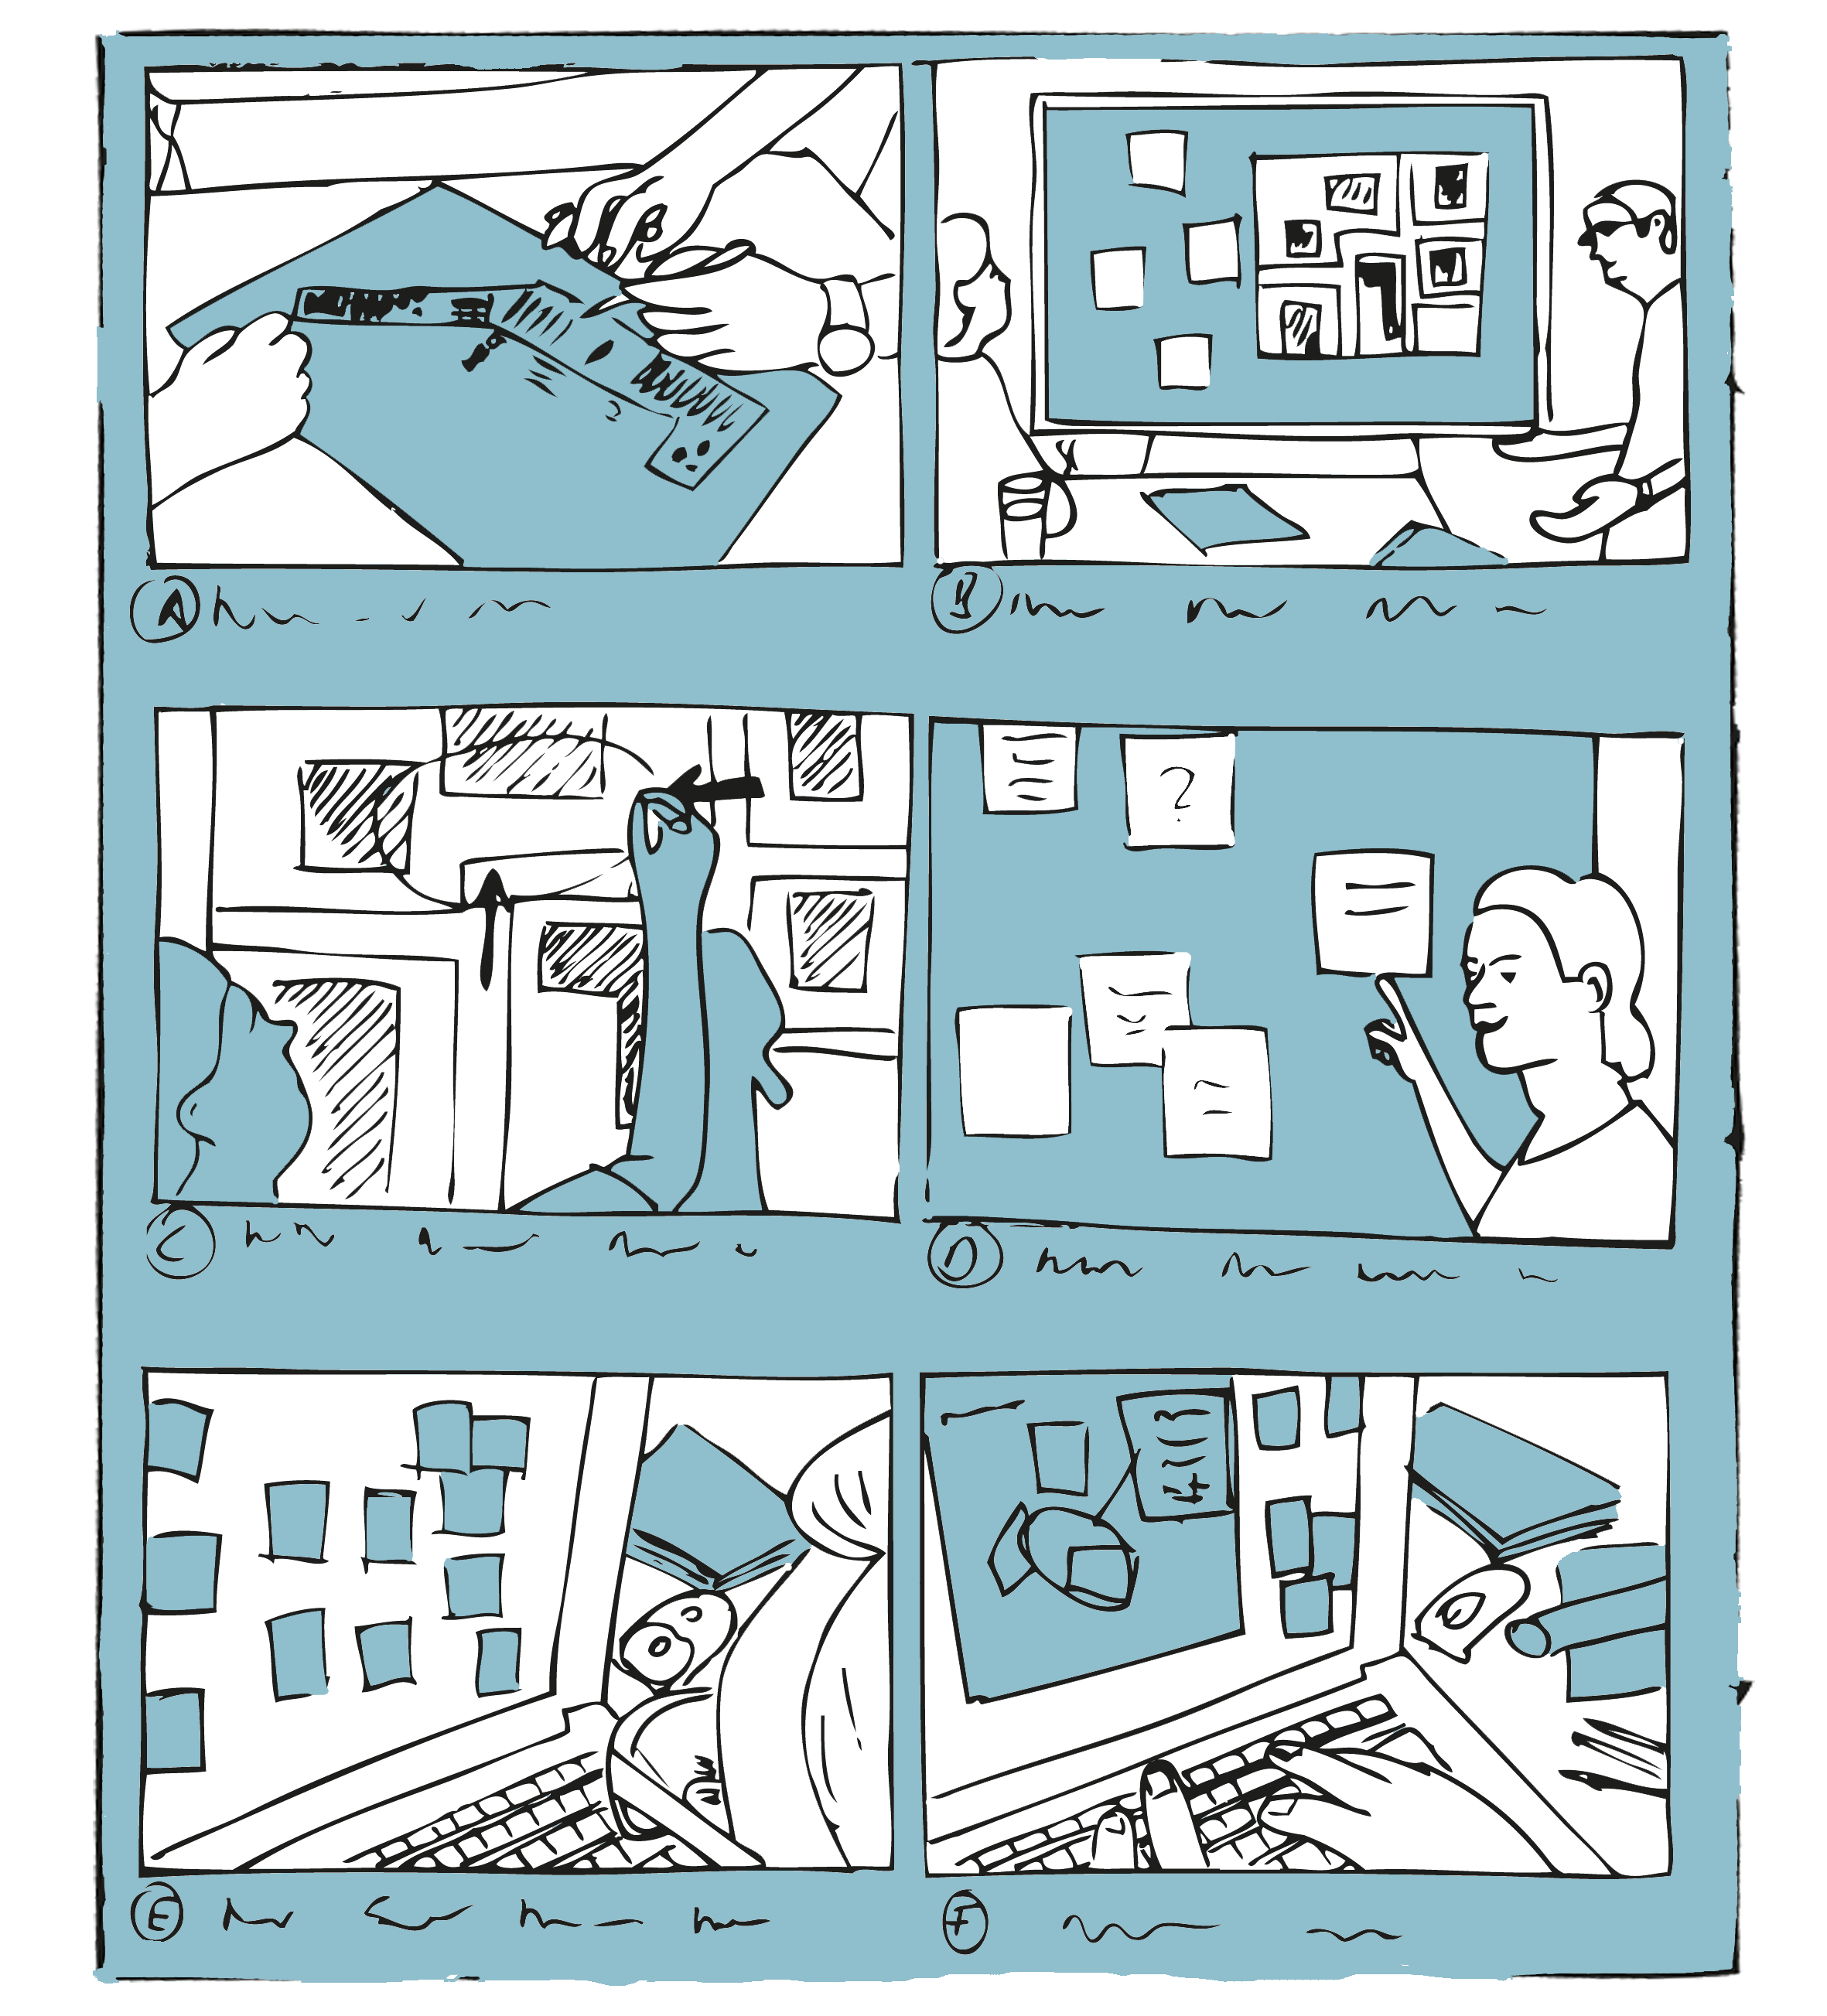
\includegraphics{Figures/07-05-Storyboard-blue-dark} \end{center}

\textbf{Arbeitsschritte}

\begin{enumerate}
\def\labelenumi{\arabic{enumi}.}
\tightlist
\item
  Festlegung/Abgrenzung der zu beschreibenden Handlung.
\item
  Sammlung von Informationen und ggf. Bildmaterial.
\item
  Bestimmung des Kontexts, der beteiligten Akteur*innen und Gegenstände.
\item
  Bestimmung zentraler Handlungsschritte/Szenen.
\item
  Ausarbeitung des Szenarios in Form eines narrativen Textes oder eines ›Storyboards‹.
\item
  Kritische Überprüfung und ggf. weitere Ausarbeitung des Szenarios.
\end{enumerate}

\textbf{Ergebnisformat}

Eine illustrative Beschreibung eines prototypischen Handlungsverlaufs, etwa in Form eines ›Storyboards‹.

\textbf{Praktische Tipps}

\begin{itemize}
\tightlist
\item
  Szenarien sollen prototypische Handlungssequenzen in einem konkreten Kontext verorten, um eine Identifikation mit den Akteuren zu ermöglichen.
\item
  Zur Veranschaulichung bieten sich Formate wie z.B. Photos \& Photomontagen an, die sich leicht modifizieren oder erweitern lassen.
\item
  Alternative Handlungsweisen sollten in getrennten Szenarien abgebildet werden.
\end{itemize}

\textbf{»Fallstricke«}

\begin{itemize}
\tightlist
\item
  Es sollte vermerkt werden, auf welchen Informationen das Szenario basiert, ob es bspw. der eigenen Erfahrung entstammt, auf Schilderungen Dritter basiert oder auch rein fiktional ist.
\item
  Bei komplexen Tätigkeiten und Vorgängen, die sehr unterschiedliche Handlungsweisen zulassen, ist es wichtig, sich auf wesentliche Handlungsschritte und Alternativen zu fokussieren.
\end{itemize}

\textbf{Weiterführende Literatur zum Leittext}

Greenberg, S., Carpendale, S., Marquardt, N. \& Buxton, B. (2012). \emph{Sketching UserExperiences -- The Workbook}. San Amsterdam: Morgan Kaufmann.

Rosson, M. \& Carroll, J. (2002). Usability Engineering: \emph{Scenario-BasedDevelopment of Human-Computer Interaction}. San Francisco: Morgan Kaufmann.

\chapter{Die Gestaltung von Technik}\label{die-gestaltung-von-technik}

Ebenso wie der Umgang mit Technik lässt sich auch die Gestaltung technischer Produkte als Teil sozialer Praktiken verstehen. Je komplexer die technischen Dinge werden, desto seltener liegen Entwurf, Herstellung und Gebrauch in einer Hand. Entsprechend sind auch die jeweiligen Praktiken mehr oder minder stark voneinander entkoppelt und durch die Ausbildung spezifischer Tätigkeitsprofile gekennzeichnet, die bis zur Ausbildung spezifischer Berufsgruppen, wie etwa von Ingenieur*innen, Architekt*innen und Softwareentwickler*innen, führen (vgl. {Abb. 8.1}).

\begin{figure}

{\centering 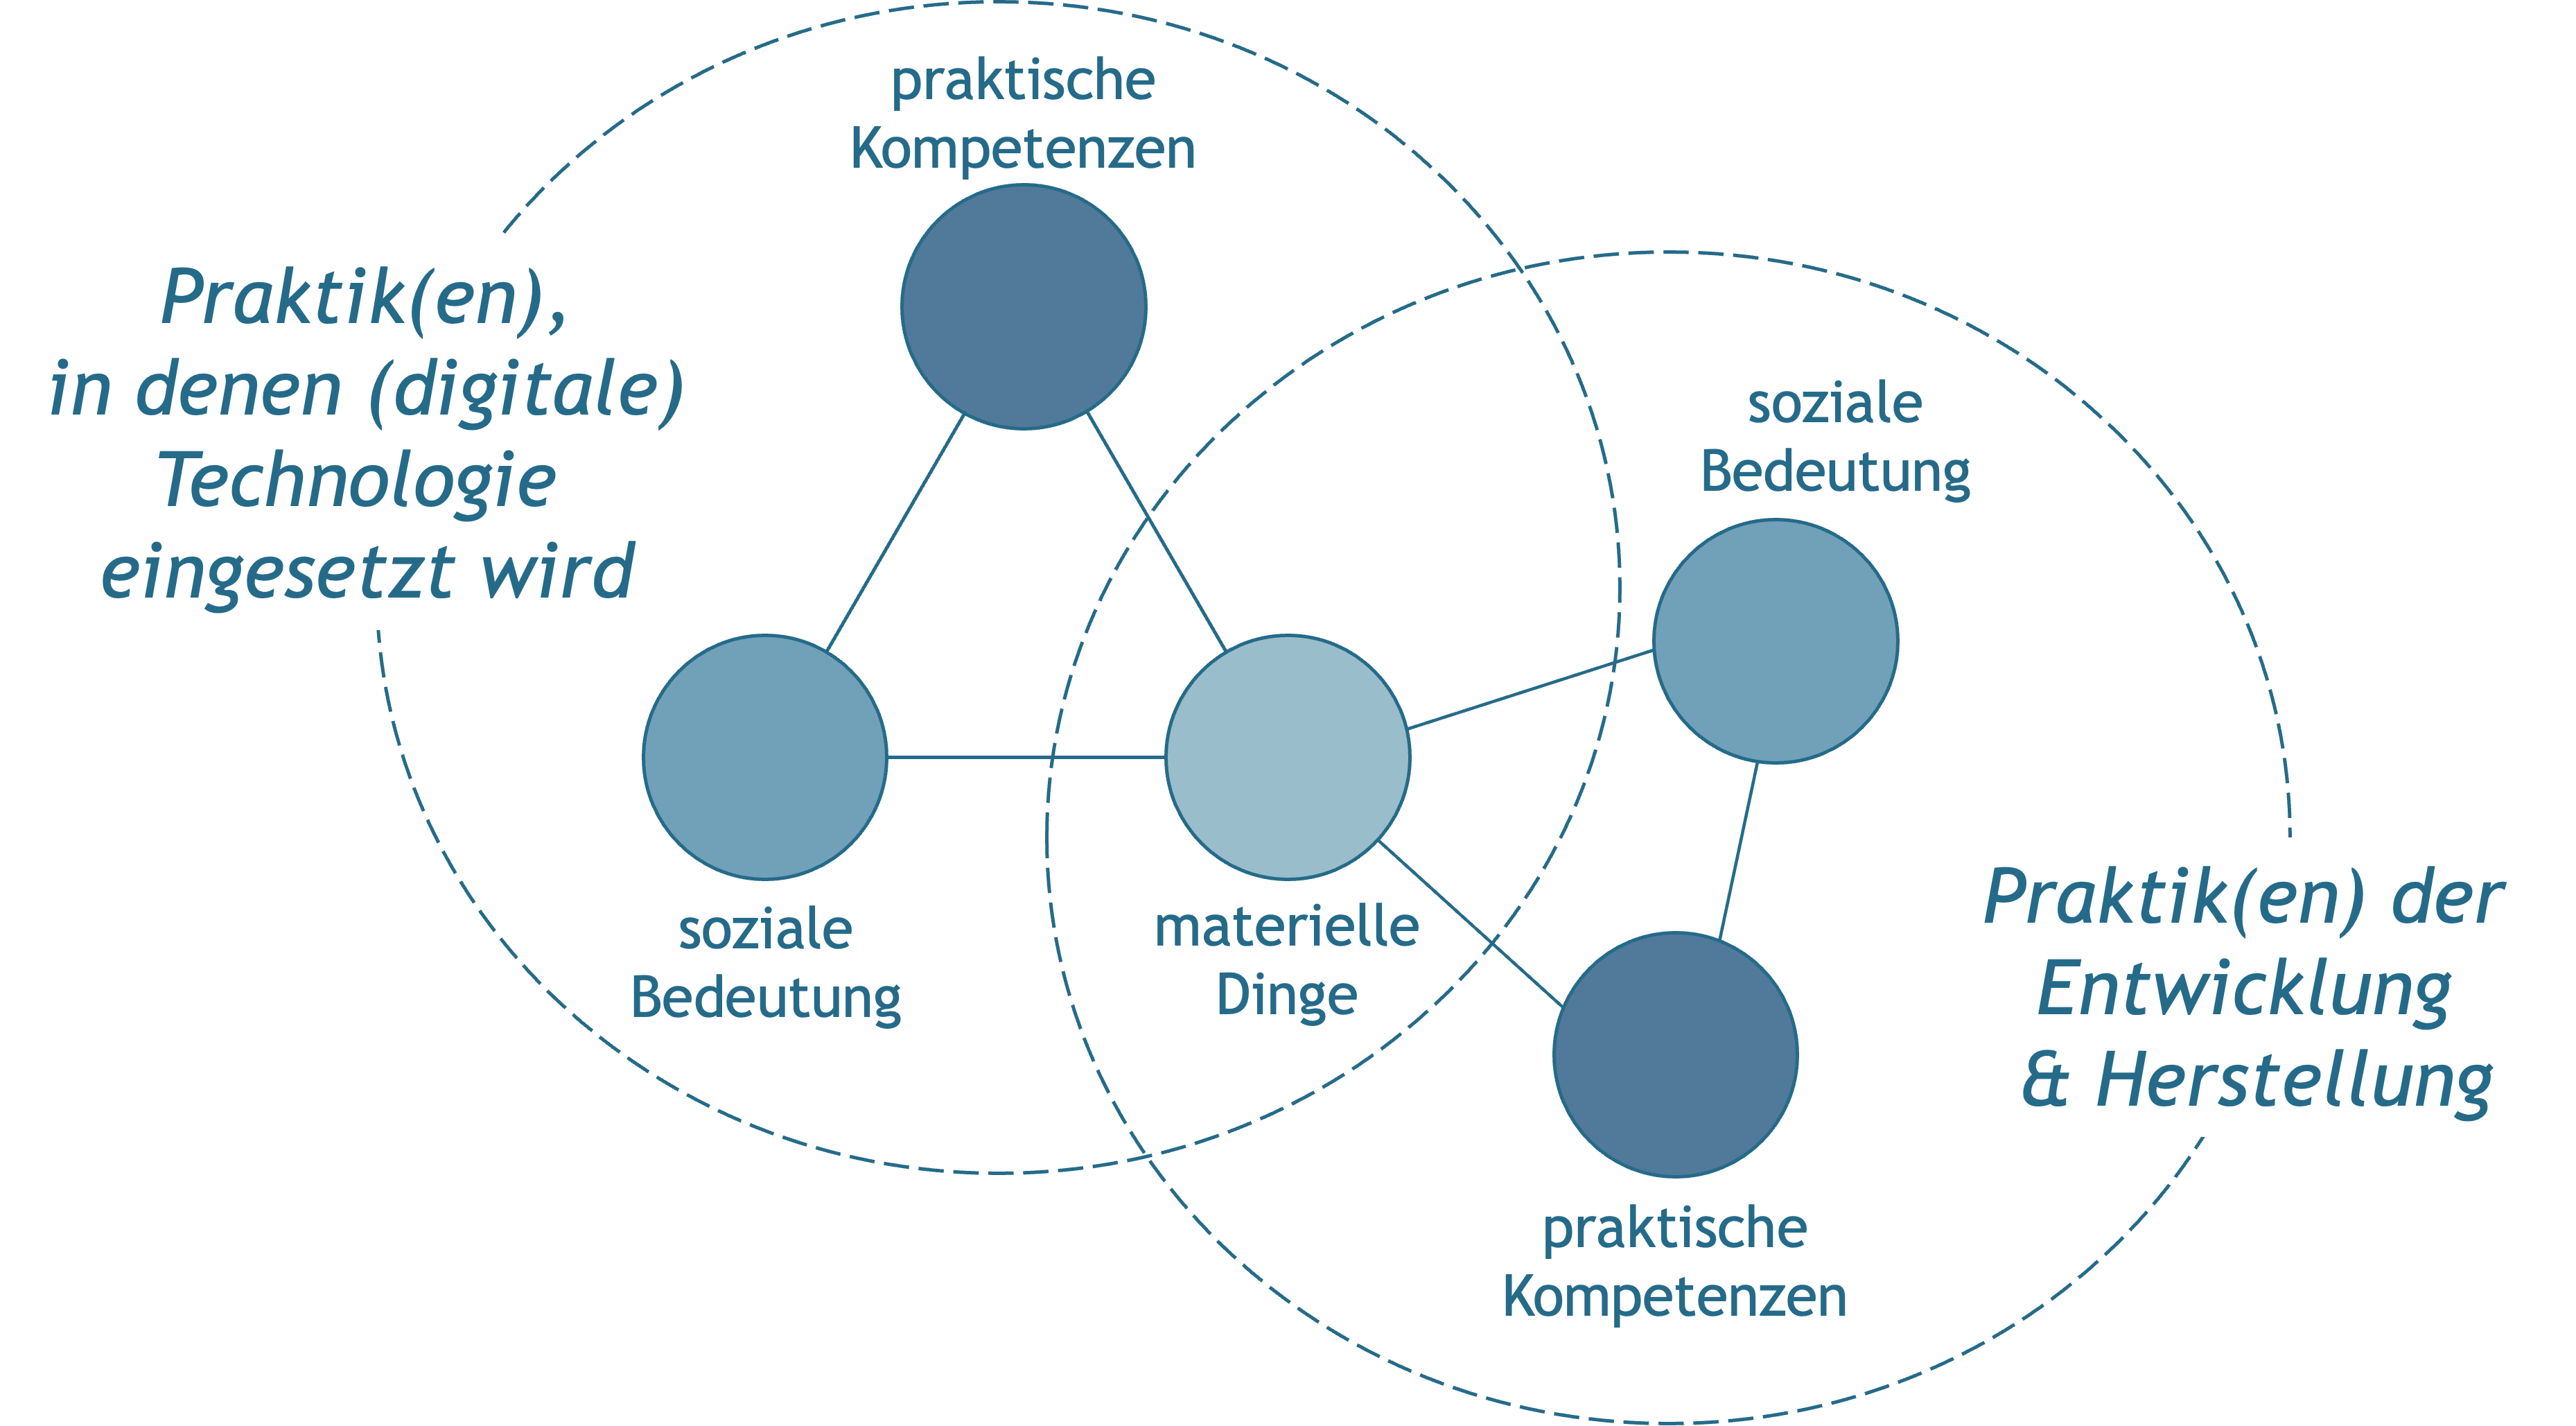
\includegraphics{Figures/08-01-gekoppelte-Praktiken} 

}

\caption{Herstellung und Gebrauch als aneinander gekoppelte Praktiken.}\label{fig:fig8}
\end{figure}

\section{Modelle als Gestaltungsprozess}\label{modelle-als-gestaltungsprozess}

Als soziale Praktik beinhaltet die Entwicklung und Herstellung technischer Produkte immer auch Annahmen und Modelle über den Sinn und Zweck wie auch die Bedingungen gestalterischen Handelns. Entsprechende Modelle bieten einen wichtigen \textbf{Orientierungsrahmen für die Praktiker*innen} und dienen gleichzeitig auch der \textbf{Vermittlung und Legitimation des eigenen Tuns gegenüber anderen}, wie etwa Auftraggeber*innen oder Anwender*innen \citep[vgl.][]{carvalhoLegitimatingDesignSociology2009, shoveDesignEverydayLife2007}.

Die Annahmen und Modelle dessen, was die Gestaltung (digitaler Technologien) ausmacht, sind nicht nur Gegenstand soziologischer und kulturwissenschaftlicher Analysen, sondern werden auch innerhalb der Ingenieurs- und Designwissenschaften, der Informatik wie auch der Pädagogik intensiv diskutiert. Über die Grenzen der einzelnen Disziplinen hinweg sind hierbei verschiedene Modelle vorgeschlagen worden, um den Gestaltungsprozess zu systematisieren und die mit ihm verbundenen Aufgaben zu definieren. Diese Modelle unterscheiden sich nicht zuletzt hinsichtlich der Frage, \textbf{was eigentlich zu gestalten ist, wie der Gestaltungsprozess organisiert} werden sollte und \textbf{welche Personengruppen} dabei in welcher Form beteiligt sein sollen. Sie umfassen immer auch mehr oder weniger explizite \textbf{Vorstellungen darüber, wie Menschen handeln} und wie sie mit technischen Dingen umgehen.

Gestaltung wird an dieser Stelle als \textbf{Oberbegriff} verstanden, der sowohl die Prozesse des \textbf{Entwerfens}, der \textbf{Konstruktion} wie auch der \textbf{Herstellung} oder \textbf{Realisierung} eines (technischen) Gegenstands umfasst. In Anlehnung an Victor Papanek \citep{papanekDesignFurReale2009} lässt sich Gestaltung dabei als »das bewusste und zugleich intuitive Bemühen um sinnvolle Ordnung« verstehen, die sich unter anderem in Form technischer Dinge manifestieren kann.

\textbf{Gestaltung als rationales Problemlösen}

Modelle der Gestaltung als Prozess des rationalen Problemlösens haben ihren Ursprung insbesondere in den Ingenieurswissenschaften. Sie gehen davon aus, dass das zu lösende Problem bereits bekannt ist und sich (im Idealfall) umfassend und präzise beschreiben lässt. Die wesentliche Aufgabe der Gestaltung besteht dementsprechend darin, unter Rückgriff auf zur Verfügung stehende Informationen eine zufriedenstellende Lösung zu finden. Eine Lösung ist dabei genau dann zufriedenstellend, wenn sie die in der Problembeschreibung festgelegten Anforderungen möglichst umfassend erfüllt. Der Gestaltungsprozess orientiert sich aus dieser Perspektive an objektiven Kriterien und ist methodisch kontrollierbar \citep[vgl.][]{lowgrenApplyingDesignMethodology1995}. Individuelle Präferenzen wie auch gesellschaftliche Normen und Werte spielen für die Suche nach einer Problemlösung keine Rolle. Ausgehend von den kognitionswissenschaftlichen Modellen der 1950er und 1960er Jahre orientieren sich diese Modelle an der Idee des Menschen als einem informationsverarbeitenden System.

\begin{figure}

{\centering 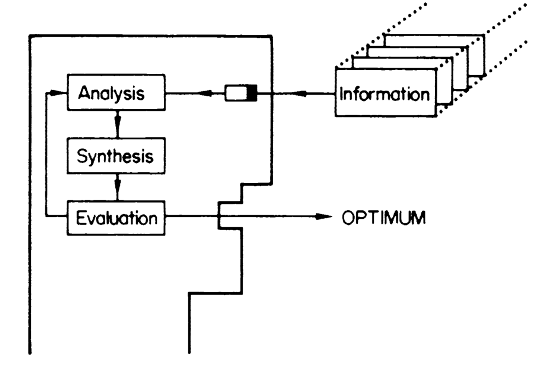
\includegraphics[width=0.75\linewidth]{Figures/08-02-Designer-als-Computer} 

}

\caption{»Designer as Computer« [aus @jonesDesignMethods1970].}\label{fig:fig9}
\end{figure}

Die Vorstellung von Gestaltung als Prozess des rationalen Problemlösens gilt als weitgehend überholt, da sie nicht zuletzt die Frage nach der Definition der zu lösenden Probleme ausklammert \citep[z.B.][]{rittelPlanningCrisisSystems1972}. Als handlungsleitendes Motiv spielt dieses Modell aber auch weiterhin eine wichtige Rolle \citep{pahlKonstruktionslehreGrundlagenErfolgreicher2007}.

\textbf{Gestaltung als kreativer und ergebnisoffener Prozess}

Modelle der Gestaltung als kreativer Prozess mit offenem Ausgang haben ihre Wurzeln vor allem in der designtheoretischen Diskussion. Im Gegensatz zur Vorstellung der Gestaltung als Problemlöseprozess gehen sie davon aus, dass sich Problemstellung und Lösung nicht voneinander trennen lassen. Jeder gestalterische Eingriff und jeder Versuch, eine Lösung zu finden, verändert vielmehr die Problemlage und zieht vorab nicht vorhersehbare Folgen nach sich. Je nachdem wie die Situation, die Anlass für einen Gestaltungsprozess gibt, verstanden wird, ergeben sich unterschiedliche Vorstellungen davon, worin das Problem besteht und wie mögliche Lösungen aussehen könnten \citep[z. B.][]{rittelPlanningCrisisSystems1972}. Gestaltung setzt aus dieser Perspektive ein Moment der Antizipation voraus, eine Vorstellung davon, was noch nicht ist, aber sein könnte und wünschenswert zu sein scheint (vgl. {Abb. 8.3}) \citep[vgl.][]{krippendorffProductSemanticsTriangulation1989, zamenopoulosAnticipatoryViewDesign2007}.

Gestaltung basiert entsprechend auf modellhaften, sozial und kulturell geprägten Vorstellungen dessen, was ist, wie auch dessen, was sein beziehungsweise werden soll, und impliziert damit immer auch normative Annahmen und Setzungen bezüglich dessen, was als wünschenswert erachtet wird.

\begin{figure}
\centering
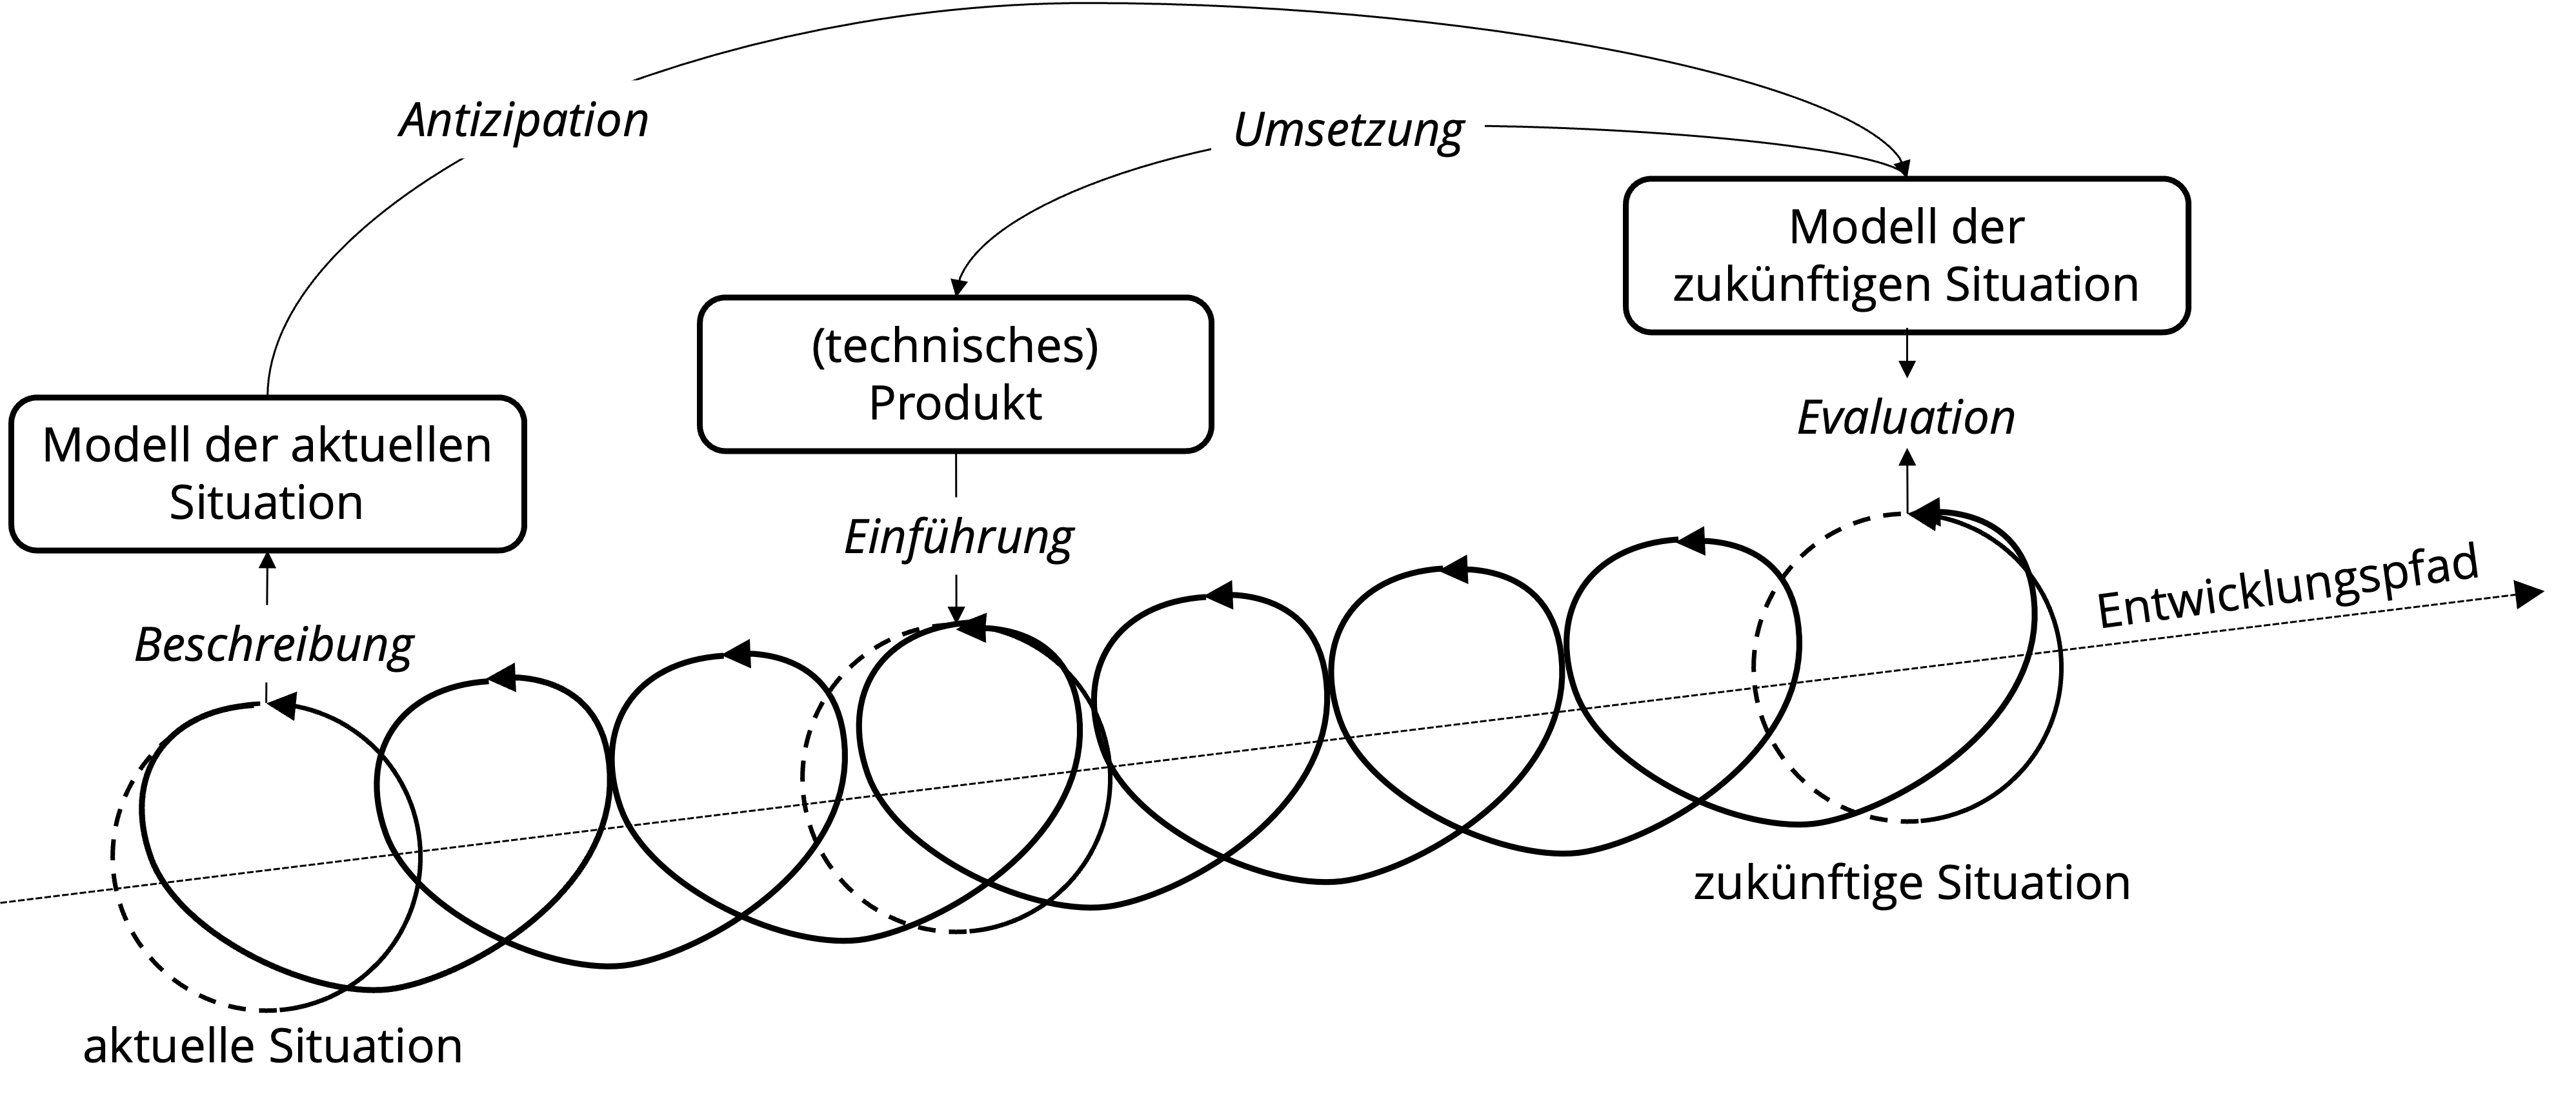
\includegraphics{Figures/08-03-Antizipation.png}
\caption{\label{fig:fig10}Gestaltung als ein antizipativer Vorgang (eigene Darstellung aufbauend auf \citet{krippendorffProductSemanticsTriangulation1989} \& \citet{zamenopoulosAnticipatoryViewDesign2007}).}
\end{figure}

\textbf{Gestaltung als koevolutionärer Prozess}

Modelle der Gestaltung als koevolutionärer Prozess finden sich in der techniksoziologischen wie auch der designtheoretischen Diskussion. Diese Ansätze erweitern den Fokus und verstehen nicht nur die Konzeption und Herstellung, sondern auch die Auswahl, Einführung und sukzessive Aneignung der jeweiligen (technischen) Produkte im Rahmen spezifischer Praktiken als Teil des Gestaltungsprozesses \citep[vgl.][]{carrollCompletingDesignUse2004}.

Herstellung und Gebrauch sind aus dieser Perspektive in rekursiver Weise aufeinander bezogen \citep[vgl.][]{bolinHeuristicsAlgorithmBig2015}. Während die Entwickler*innen an bereits bestehenden Praktiken, Routinen und Produkten anknüpfen und ein Modell zukünftiger Anwendungsmöglichkeiten entwerfen, eignen sich die Praktiker*innen ihnen zur Verfügung stehende oder gestellte Produkte aktiv an, indem sie diese erproben, hinsichtlich ihrer ›Praxistauglichkeit‹ evaluieren und, soweit möglich und erforderlich, ihren jeweiligen Bedürfnissen anpassen (vgl. {Abb. 8.4}).

Aus evolutionstheoretischer Sicht produziert die Konzeption und Herstellung (technischer) Produkte in Bezug auf die Transformation sozialer Praktiken Variation: Eine Bandbreite neuer Produkte wird verfügbar, die sich aber erst noch als praxistauglich erweisen müssen (Selektion), bevor sie zu einem fixen Bestandteil einer veränderten, sozialen Praktik werden können (Re-Stabilisierung) \citep[vgl.][]{jonasDesignResearchIts2007}.

\begin{figure}
\centering
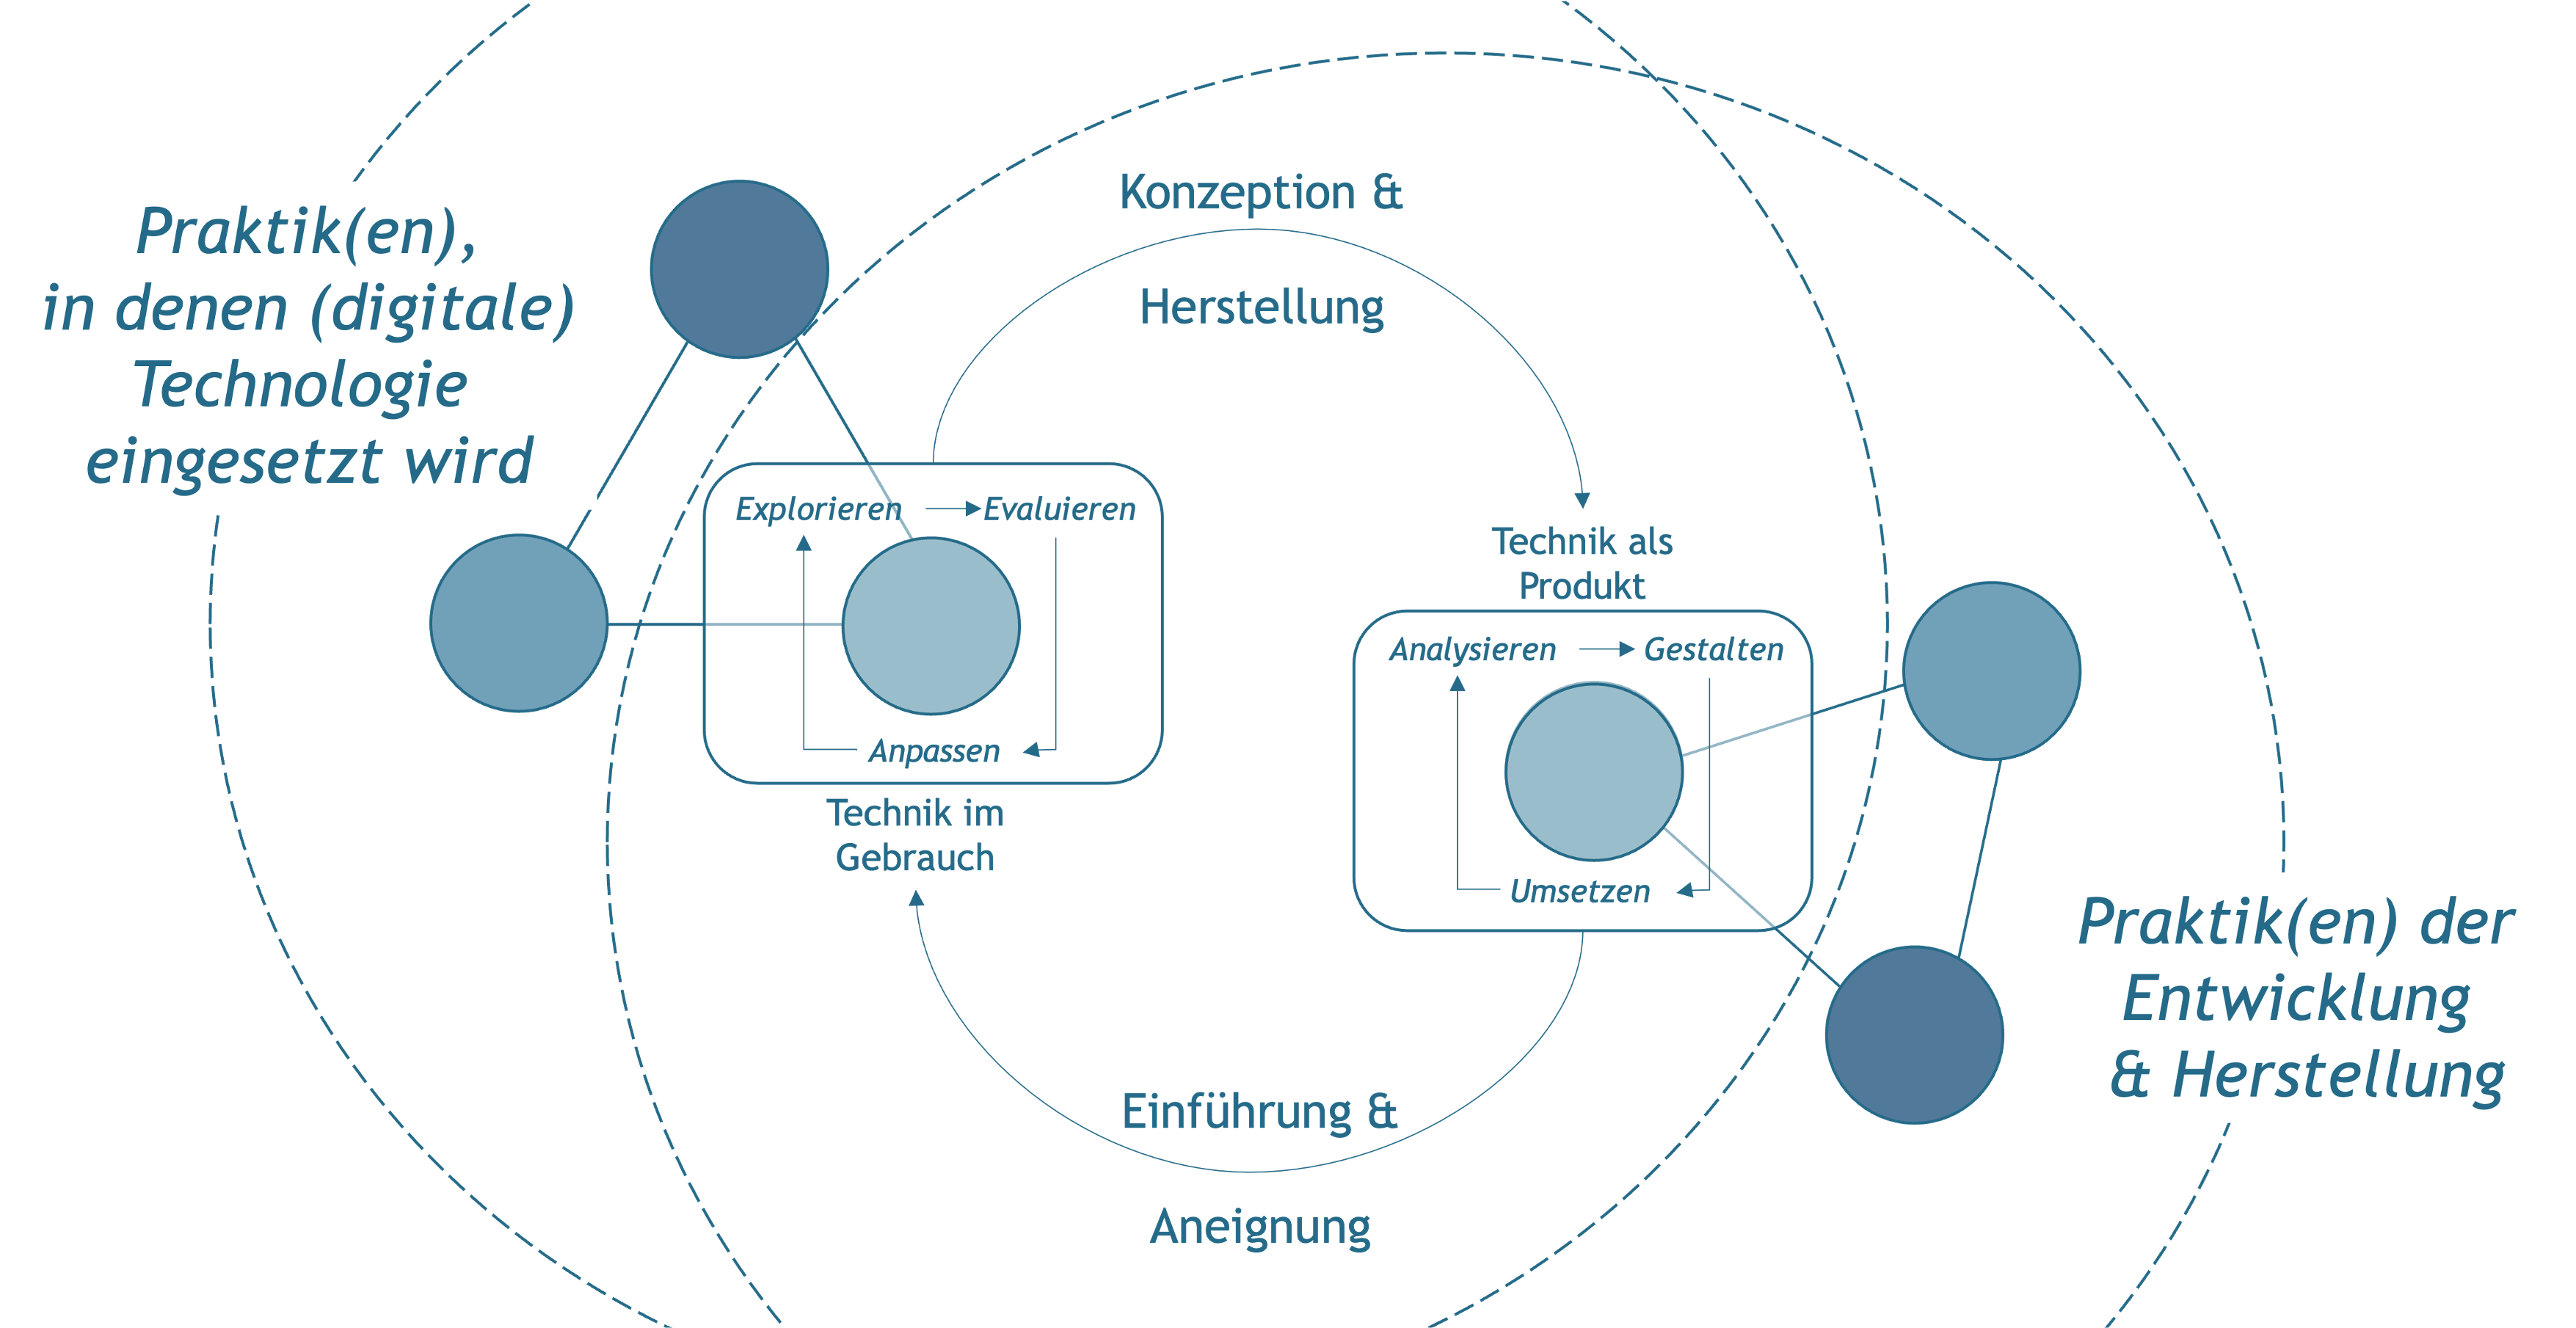
\includegraphics{Figures/08-04-Gestaltung-Wechselspiel.png}
\caption{\label{fig:fig11}Gestaltung im Wechselspiel von Konzeption, Herstellung, Einführung und Aneignung (eigene Darstellung aufbauend auf \citet{bolinHeuristicsAlgorithmBig2015} \& \citet{shoveDynamicsSocialPractice2012}).}
\end{figure}

\begin{blackbox}
\emph{Welche Beispiele für die aktive Umnutzung oder Zweckentfremdung technischer Produkte begegnen Ihnen in Ihrem Alltag? Wie kommt es dazu?}

\end{blackbox}

\section{Rekonstruktion der Produktvision}\label{rekonstruktion-der-produktvision}

\textbf{Ziel}

Die Rekonstruktion der Produktvision dient dazu, die einem Produkt zugrundeliegenden Annahmen der Entwickler*innen zu identifizieren.

\textbf{Leitgedanke}

Die Rekonstruktion der Produktvision geht davon aus, dass die an der Gestaltung eines Produkts beteiligten Personen eine bestimmte Perspektive auf den Gegenstandsgegenstand entwickelt haben, auf deren Grundlage sie ihre Entscheidungen treffen. Die Produktvision umfasst dabei insbesondere Aussagen über den Zweck und Mehrwert des Produkts, die Zielgruppe und ihre Bedürfnisse wie auch zentrale Anwendungsfälle und Funktionen. Grundlage für die Rekonstruktion können u.a. Produktwebseiten, Werbematerialien, Anleitungen, Pressemitteilungen und Entwicklerblogs sein.

\textbf{Anwendungskontext}

Ausgangspunkt für die Rekonstruktion bilden die Aussagen der Entwickler*innen über ein konkretes Produkt. Die rekonstruierte Produktversion bietet einen Referenzpunkt zum Abgleich mit tatsächlichen Nutzungsformen.

\begin{center}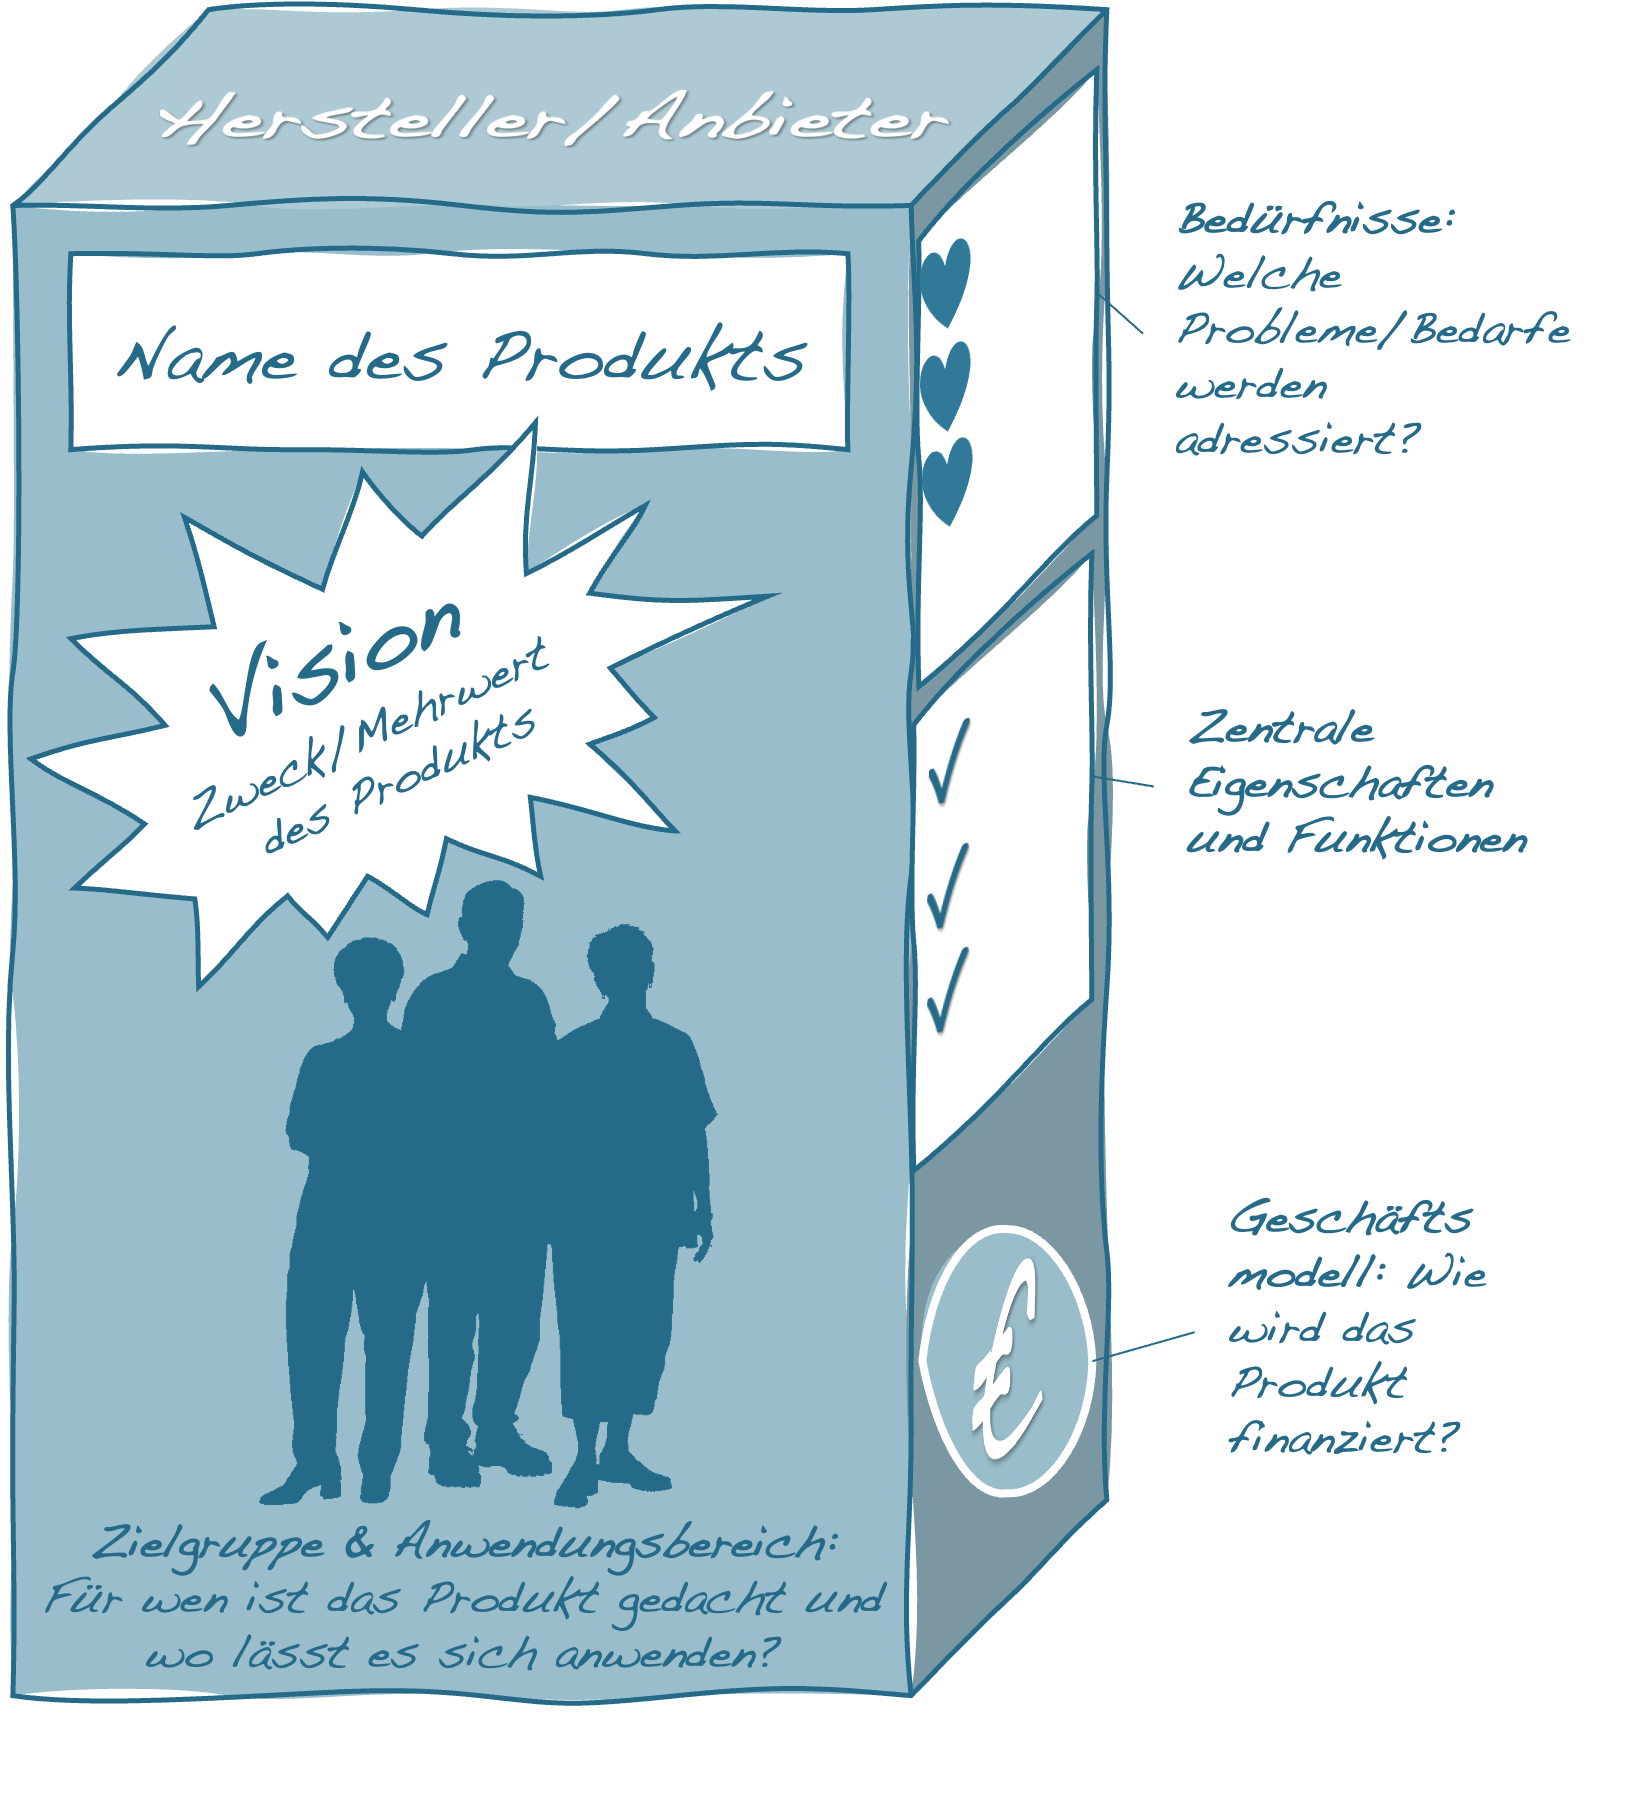
\includegraphics{Figures/08-05-Produktvision} \end{center}

\textbf{Arbeitsschritte}

\begin{enumerate}
\def\labelenumi{\arabic{enumi}.}
\tightlist
\item
  Auswahl des Produkts.
\item
  Sammlung von Darstellungen des Produkts durch die Entwickler*innen, z.B. Produktwebseiten, Werbematerialien, Anleitungen, Entwicklerblogs.
\item
  Abgleich und Verdichtung der gesammelten Aussagen.
\item
  Zusammenfassung in Form einer Produktpräsentation.
\item
  Kritische Überprüfung und ggf. weitere Ausarbeitung des Szenarios.
\end{enumerate}

\textbf{Ergebnisformat}

Darstellung der Produktvision in Form einer fiktiven Produktverpackung.

\textbf{Praktische Tipps}

\begin{itemize}
\tightlist
\item
  Im Mittelpunkt stehen die Intentionen und Ideen der Entwickler*innen. Ob und wie gut diese tatsächlich realisiert werden konnten, ist zunächst nicht relevant.
\item
  Die Rekonstruktion sollte sich soweit als möglich an den Begrifflichkeiten und Darstellungsweisen der Entwickler*innen orientieren.
\item
  Zur besseren Nachvollziehbarkeit sollten die verwendeten Quellen dokumentiert werden.
\end{itemize}

\textbf{»Fallstricke«}

\begin{itemize}
\tightlist
\item
  Da die Produktvision auf Annahmen beruht, ist sie weder wahr noch falsch, sondern in erster Linie Ausdruck einer bestimmten Position oder Haltung.
\item
  Nicht alle produktbezogenen Annahmen müssen explizit benannt werden. Auch visuelle Darstellungen, z.B. von Anwender*innen, oder Beispiele können auf Annahmen hinweisen.
\end{itemize}

\textbf{Weiterführende Literatur zum Leittext}

Deasy, D. (2003). Non-AssumptiveResearch. In B. Laurel (ed). \emph{Design Research --Methods and Perspectives} (pp.~172-174), MITPress.

Highsmith, J. A. (2004). \emph{Agile project management: Creating innovative products}. Addison-Wesley.

Light, B., Burgess, J., \& Duguay, S. (2018). The walkthrough method: An approach to the study of apps. \emph{New Media \& Society}, 20(3), 881--900.

\chapter{Modellierung und Formalisierung}\label{modellierung-und-formalisierung}

Ein wesentliches Moment digitaler Technologien besteht in der \textbf{automatisierten Ausführung und Steuerung praktisch relevanter Vorgänge} auf Basis von Algorithmen. Die Entwicklung digitaler Technologien setzt dementsprechend voraus, dass die zu automatisierenden Vorgänge in einer Weise beschrieben werden, die von einem Computer verarbeitet werden können. Zentrale Grundlage hierfür bildet die \textbf{formale Modellierung des jeweiligen Anwendungsbereichs}.

Diejenigen, die an der Entwicklung einer digitalen Technologie beteiligt sind, entwickeln dabei Modelle, sowohl der aktuellen Situation wie auch einer antizipierten Zukunft. Ein zentraler Gegenstand der Modellierung sind dabei jene Praktiken, innerhalb derer das jeweilige Produkt zum Einsatz kommen soll.

\begin{figure}

{\centering 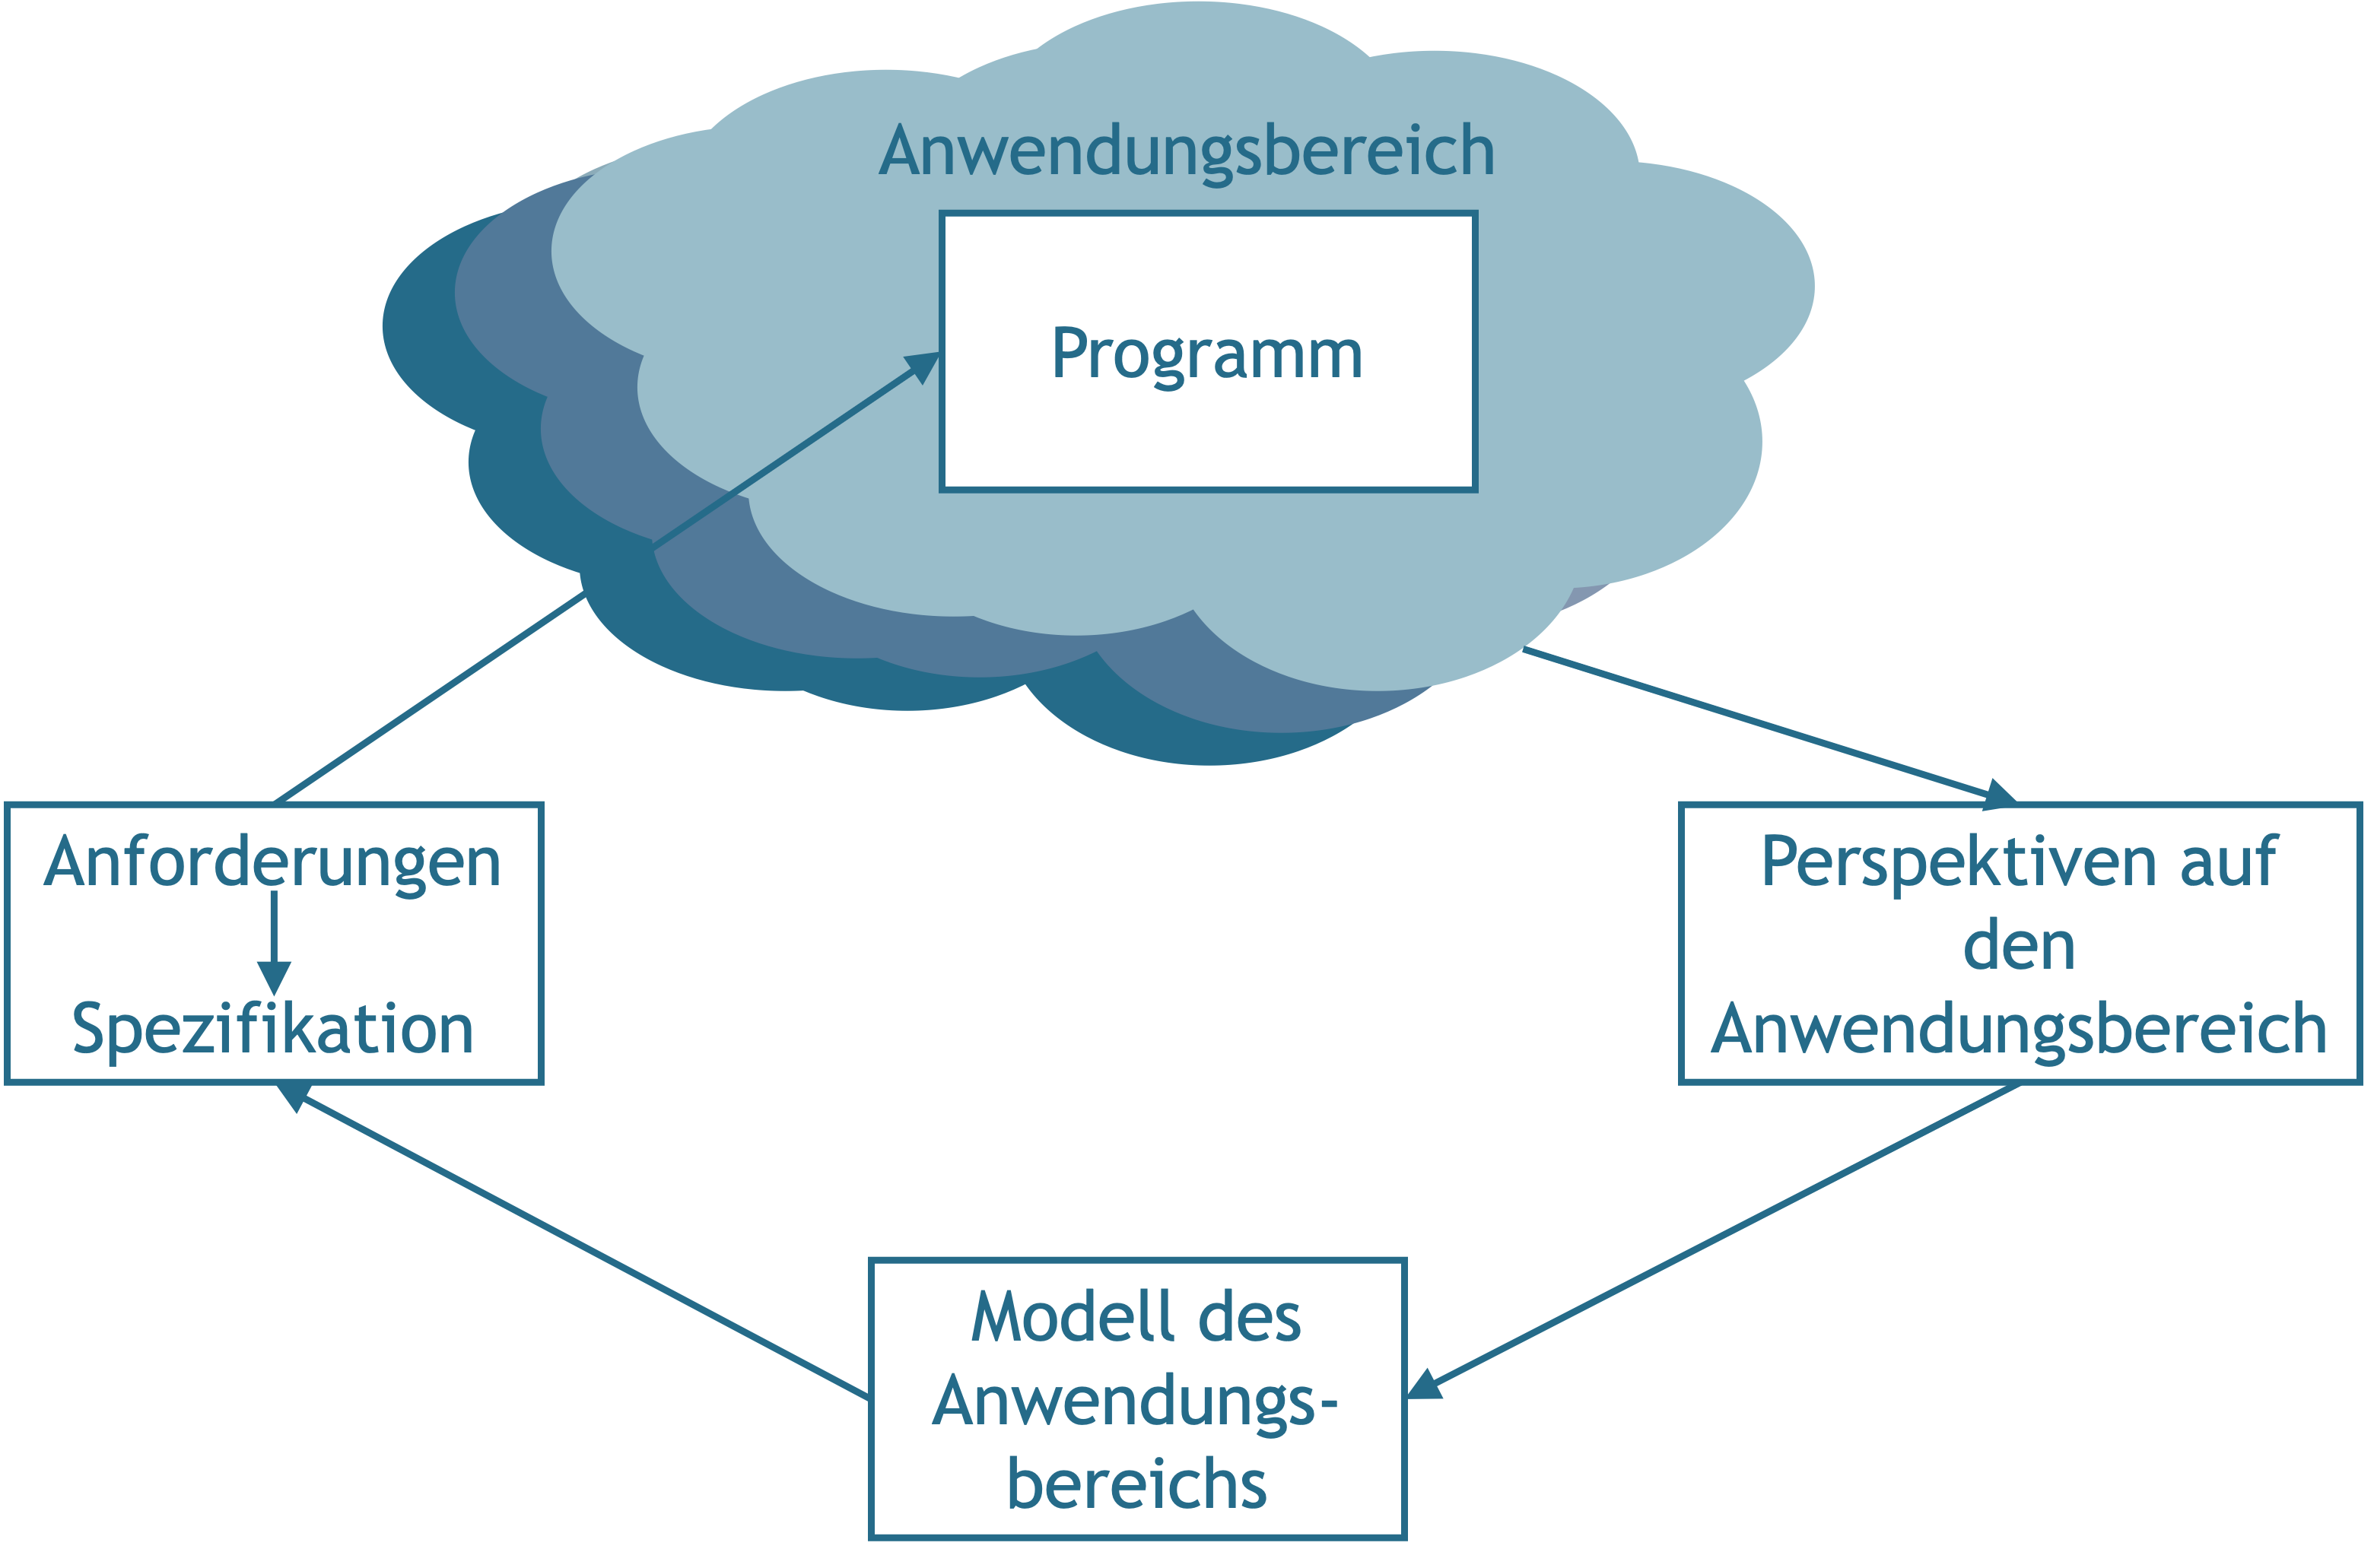
\includegraphics[width=0.75\linewidth]{Figures/09-01-Modellbildung} 

}

\caption{»Any program is a model of a model within a theory of a model of an abstraction of some portion of the world or of some universe of discourse.« [@lehmanProgramsLifeCycles1980, S. 1061].}\label{fig:fig12}
\end{figure}

\section{Modellierung und Formalisierung als Voraussetzungen der Digitalisierung}\label{modellierung-und-formalisierung-als-voraussetzungen-der-digitalisierung}

\begin{figure}

{\centering 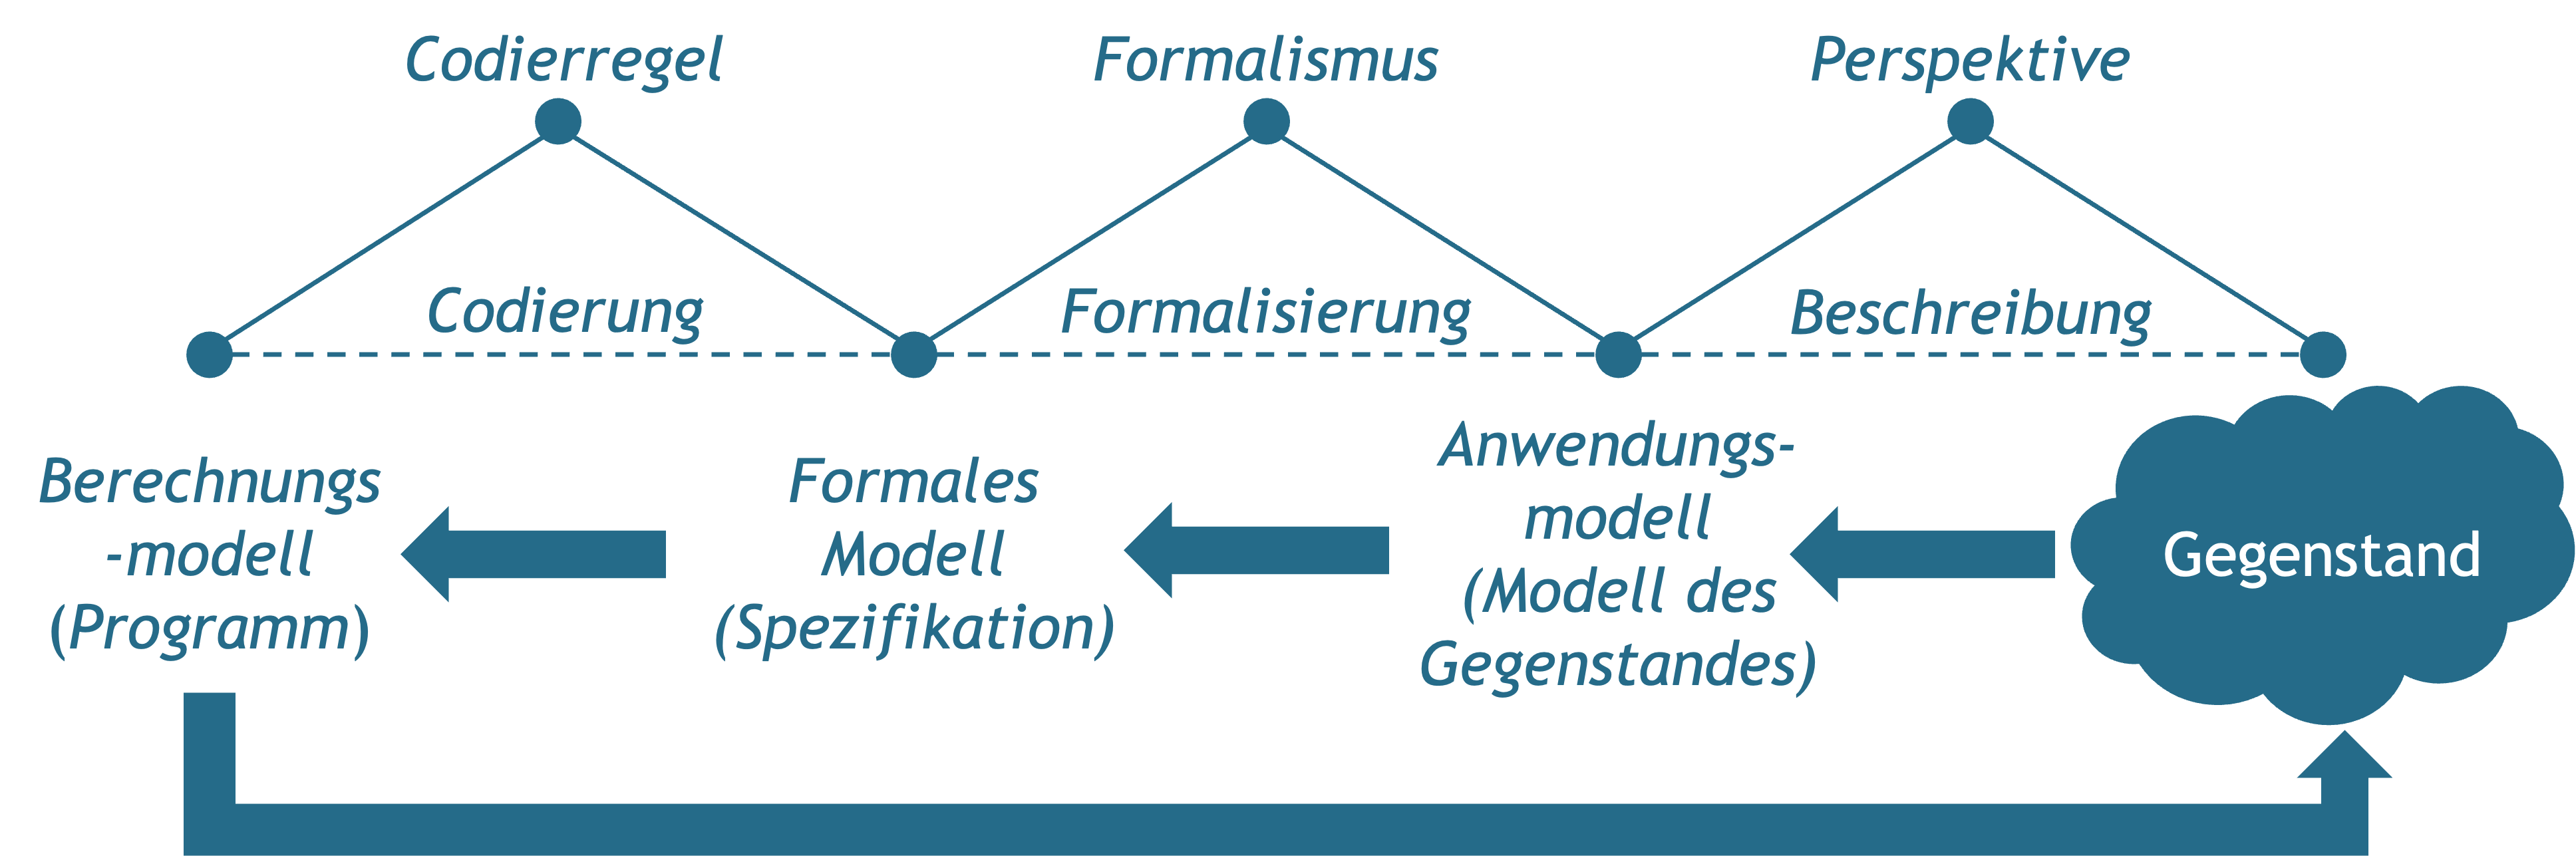
\includegraphics{Figures/09-02-InformatischeModellbildung} 

}

\caption{Programmierung als ein mehrstufiger Übersetzungsprozess.}\label{fig:fig13}
\end{figure}

Das Programmieren und damit auch die Entwicklung digitaler Dinge lässt sich im Kern als ein \textbf{Prozess der Modellierung} verstehen (siehe {Abb. 9.1}). Das von einem Computer ausführbare Programm ist letztendlich ein Modell, eine Beschreibung für die Lösung einer Aufgabe, die so formuliert ist, dass sie von einem Computer ausgeführt werden kann \citep{floydModellierungHandgriffZur1998, humbertInformatikUbergreifendeEinzigartige2002, rechenbergInformatikHandbuch2002}.

Ein \textbf{Programm} ist insofern ein \textbf{›Berechnungsmodell‹}, das darstellt, wie Daten zu verarbeiten sind, damit ein bestimmtes Ergebnis erzielt werden kann. Damit ein Programm von einem Computer verarbeitet werden kann, muss es so formuliert sein, dass die Anwendung der im Programm beschriebenen Regeln eindeutig ist und unabhängig von der Bedeutung der zu verarbeitenden Daten erfolgen kann. Ein Programm setzt somit bereits ein \textbf{formales Modell} der Aufgabe wie auch der Lösung voraus. Das, was das Programm leisten soll, muss deshalb im Rahmen einer \textbf{›Spezifikation‹} eindeutig definiert sein. Da jedoch handlungspraktische Situationen und die mit ihnen einhergehenden \textbf{›Aufgaben‹} nicht eindeutig definiert sind, sondern in unterschiedlicher Weise interpretiert und beschrieben werden können, geht (zumindest im Fall anwendungsbezogener Programme) der Spezifikation bereits eine Modellierung des Anwendungsbereichs voraus. Entsprechende \textbf{›Anwendungsmodelle‹} implizieren dabei immer auch eine bestimmte Vorstellung davon, wie der Gegenstandsbereich organisiert ist.

Der Prozess des Programmierens lässt sich dementsprechend als ein mehrstufiger Vorgang verstehen (siehe {Abb. 9.2}). Ausgehend von einem konkreten Gegenstand oder einer Situation wird zunächst ein Anwendungsmodell erstellt, aus dem hervorgeht, welche Aspekte des Gegenstandsbereichs als relevant und welche Zustände als (nicht) wünschenswert betrachtet werden. Dieses Anwendungsmodell wird dann in eine formale Spezifikation überführt, aus der hervorgeht, was ein entsprechendes Programm leisten soll, bevor dieses dann in einem Berechnungsmodell realisiert werden kann. Da die verschiedenen Modellarten nicht direkt ineinander überführt werden können, bedarf es jeweils einer \textbf{›Übersetzung‹}, mittels derer die unterschiedlichen Modelle miteinander in Beziehung gesetzt werden \citep[siehe hierzu ausführlicher][]{haeusslingZurRolleEntwuerfen2016}.

\section{Von situierten Handlungsabläufen zur ›autooperationalen Form‹}\label{von-situierten-handlungsabluxe4ufen-zur-autooperationalen-form}

Die Vorstellung der Programmierung wie auch der Entwicklung digitaler Technologien als Prozess der Modellierung lässt zunächst offen, was eigentlich modelliert und formalisiert wird. Hiermit verbunden ist die Frage, ob es in der Informatik eine bestimmte Vorstellung davon gibt, wie der Gegenstandsbereich organisiert ist. Eine mögliche Antwort auf diese Frage liefert die von der Informatikerin Christiane Floyd aufgestellte These, dass »Informatik {[}\ldots{]} in beliebigen Bereichen menschlicher Praxis {[}eingreift{]} und {[}\ldots{]} den jeweils interessierenden Bereich als \textbf{operationale Form} {[}begreift{]}« \citep[S. 238]{floydAutooperationaleFormUnd1997}.

Unter einer operationalen Form versteht Floyd dabei »eine Struktur aus möglichen Operationen in einem interessierenden Gegenstandsbereich« \citep[S. 242]{floydAutooperationaleFormUnd1997}. Im Gegensatz zum praktischen Vollzug ist die Operation dabei kein Prozess, sondern die Beschreibung eines Prozesses und damit ein Modell. Entsprechend lässt sich etwa ein Rezept zum Backen von Pfannkuchen oder die Bedienungsanleitung einer Waschmaschine als operationale Form verstehen. Ein wesentliches Charakteristikum der operationalen Form ist ihre Übertragbarkeit, denn »{[}e{]}s geht darum, Schritte des Vollzugs so zu charakterisieren, dass ihre Voraussetzungen und Ergebnisse sowie ihre Randbedingungen geklärt sind, um sie wiederholbar und planbar zu machen« \citep[S. 242]{floydAutooperationaleFormUnd1997}. Die Übersetzung situierter Handlungsabläufe in operationale Formen bezeichnet Floyd als operationale Rekonstruktion. Mittels Formalisierung lassen sich operationale Formen dann zunächst in Algorithmen und mittels Codierung in \textbf{autooperationale Formen} übersetzen, die von einem Computer ausgeführt werden können (siehe {Abb. 9.3}).

Entscheidend an der Argumentation von Floyd ist, dass operationale Rekonstruktionen zugleich reduktiv wie auch produktiv sind. Operationale Rekonstruktionen sind einerseits \textbf{reduktiv}, da sie von den Details des Einzelfalls abstrahieren und sich auf das vermeintlich Wesentliche und Regelhafte konzentrieren. Andererseits sind sie \textbf{produktiv}, da sie neue und ausdifferenziertere Praktiken ermöglichen. So limitiert etwa ein Texteditor den verfügbaren Zeichensatz, macht es aber möglich ein und denselben Satz immer wieder zu verändern, ohne dabei sichtbare Spuren zu hinterlassen. Die (auto-)operationalen Formen wirken auf diese Weise auf die jeweiligen Praktiken zurück und transformieren diese.

\begin{figure}

{\centering 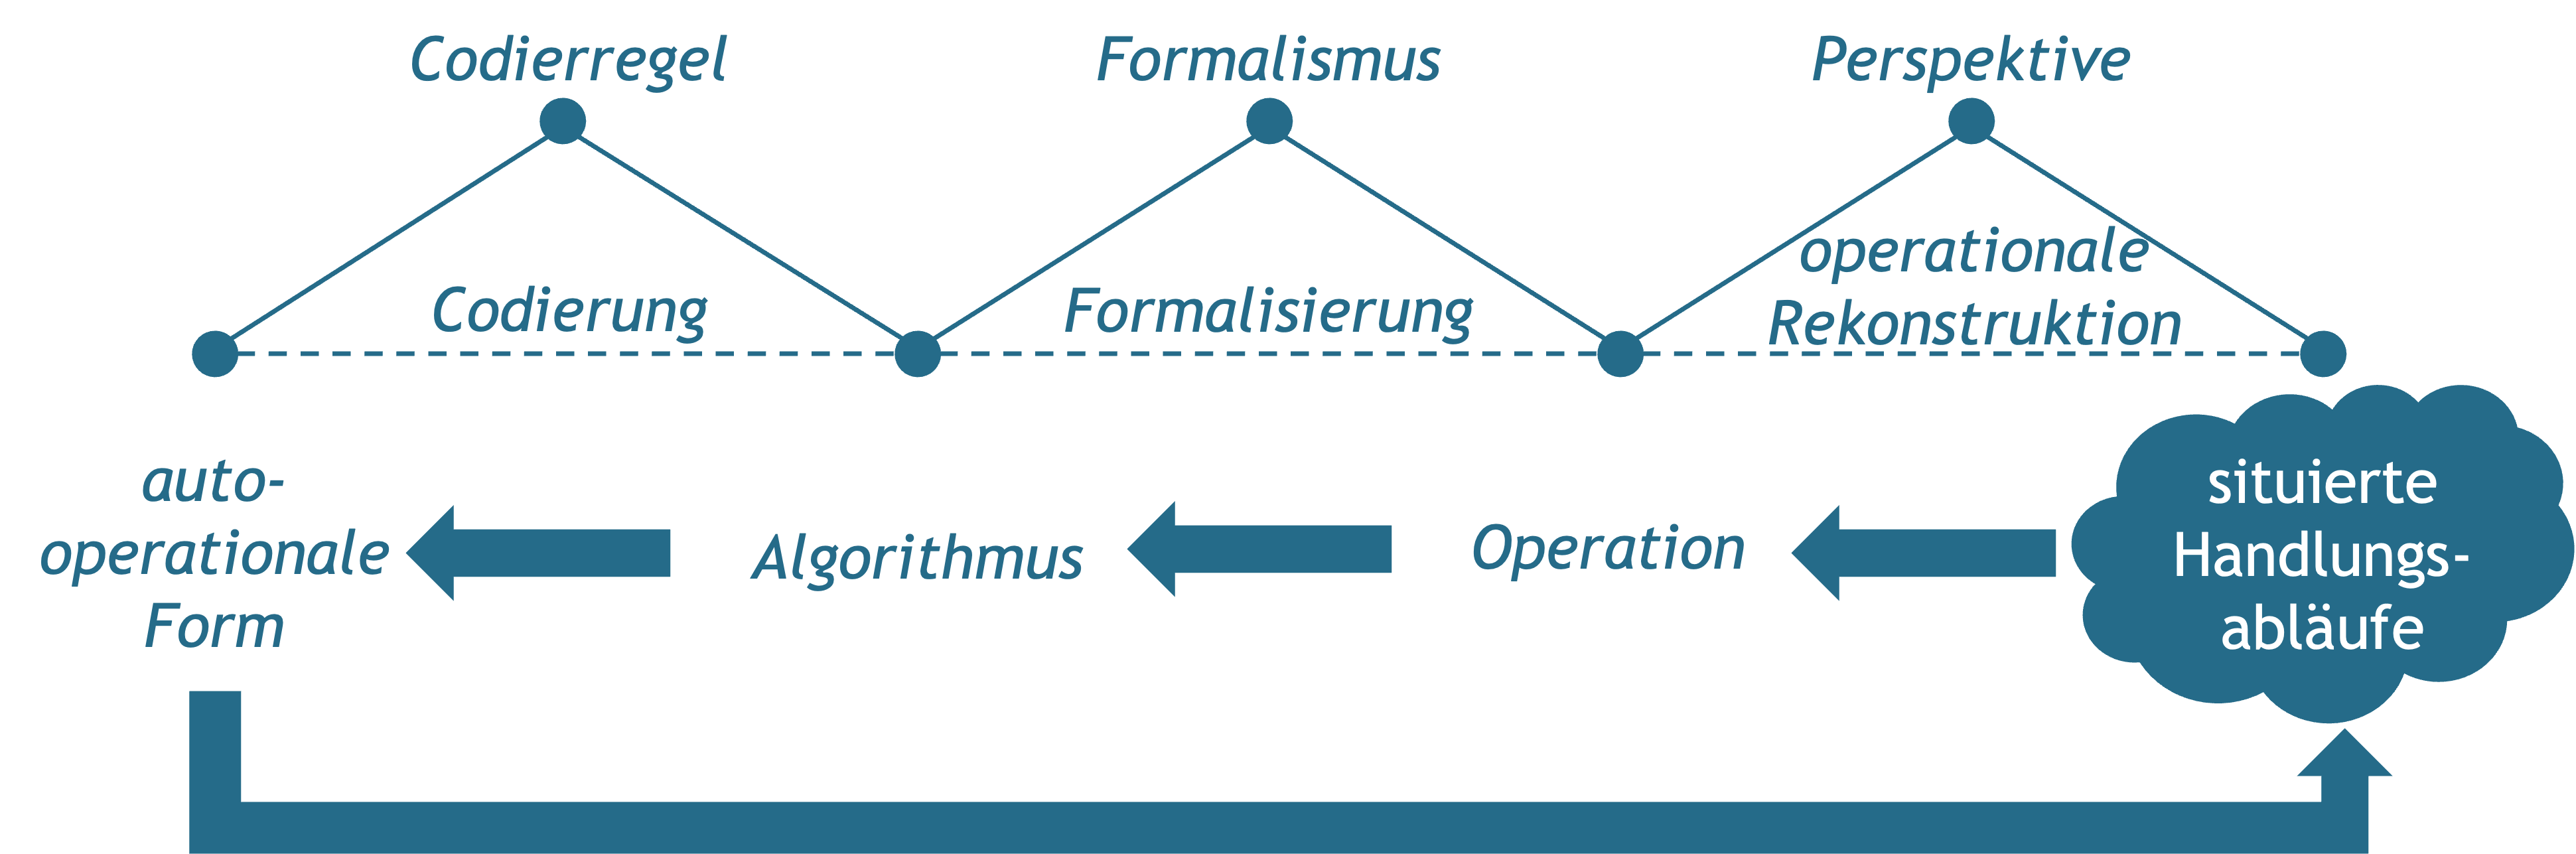
\includegraphics{Figures/09-03-autooperationaleForm} 

}

\caption{Übersetzungsschritte von situierten Handlungsabläufen zur autooperationalen Form.}\label{fig:fig14}
\end{figure}

\section{Beispiel \& Diskussionspunkt Antolin}\label{beispiel-diskussionspunkt-antolin}

Die für die Entwicklung digitaler Produkte notwendigen ›Übersetzungen‹ lassen sich an \href{https://antolin.westermann.de/}{Antolin} als einer Plattform zur Leseförderung exemplarisch veranschaulichen. Im Mittelpunkt der folgenden Rekonstruktion steht dabei die auf Antolin realisierte Überprüfung des Leseverständnisses der Schüler*innen mittels einer Reihe von Multiple-Choice-Fragen zu den jeweils gelesenen Büchern.

Dieser Prozess ist im Kontext von Antolin zentral, da sich an ihm die Punktevergabe und damit die ›Vermessung‹ des Leseverhaltens der Schüler*innen festmacht.

Hinsichtlich der Überführung situierter Handlungsabläufe in eine ›autooperationale Form‹, lassen sich folgende Übersetzungsschritte ausmachen:

\begin{center}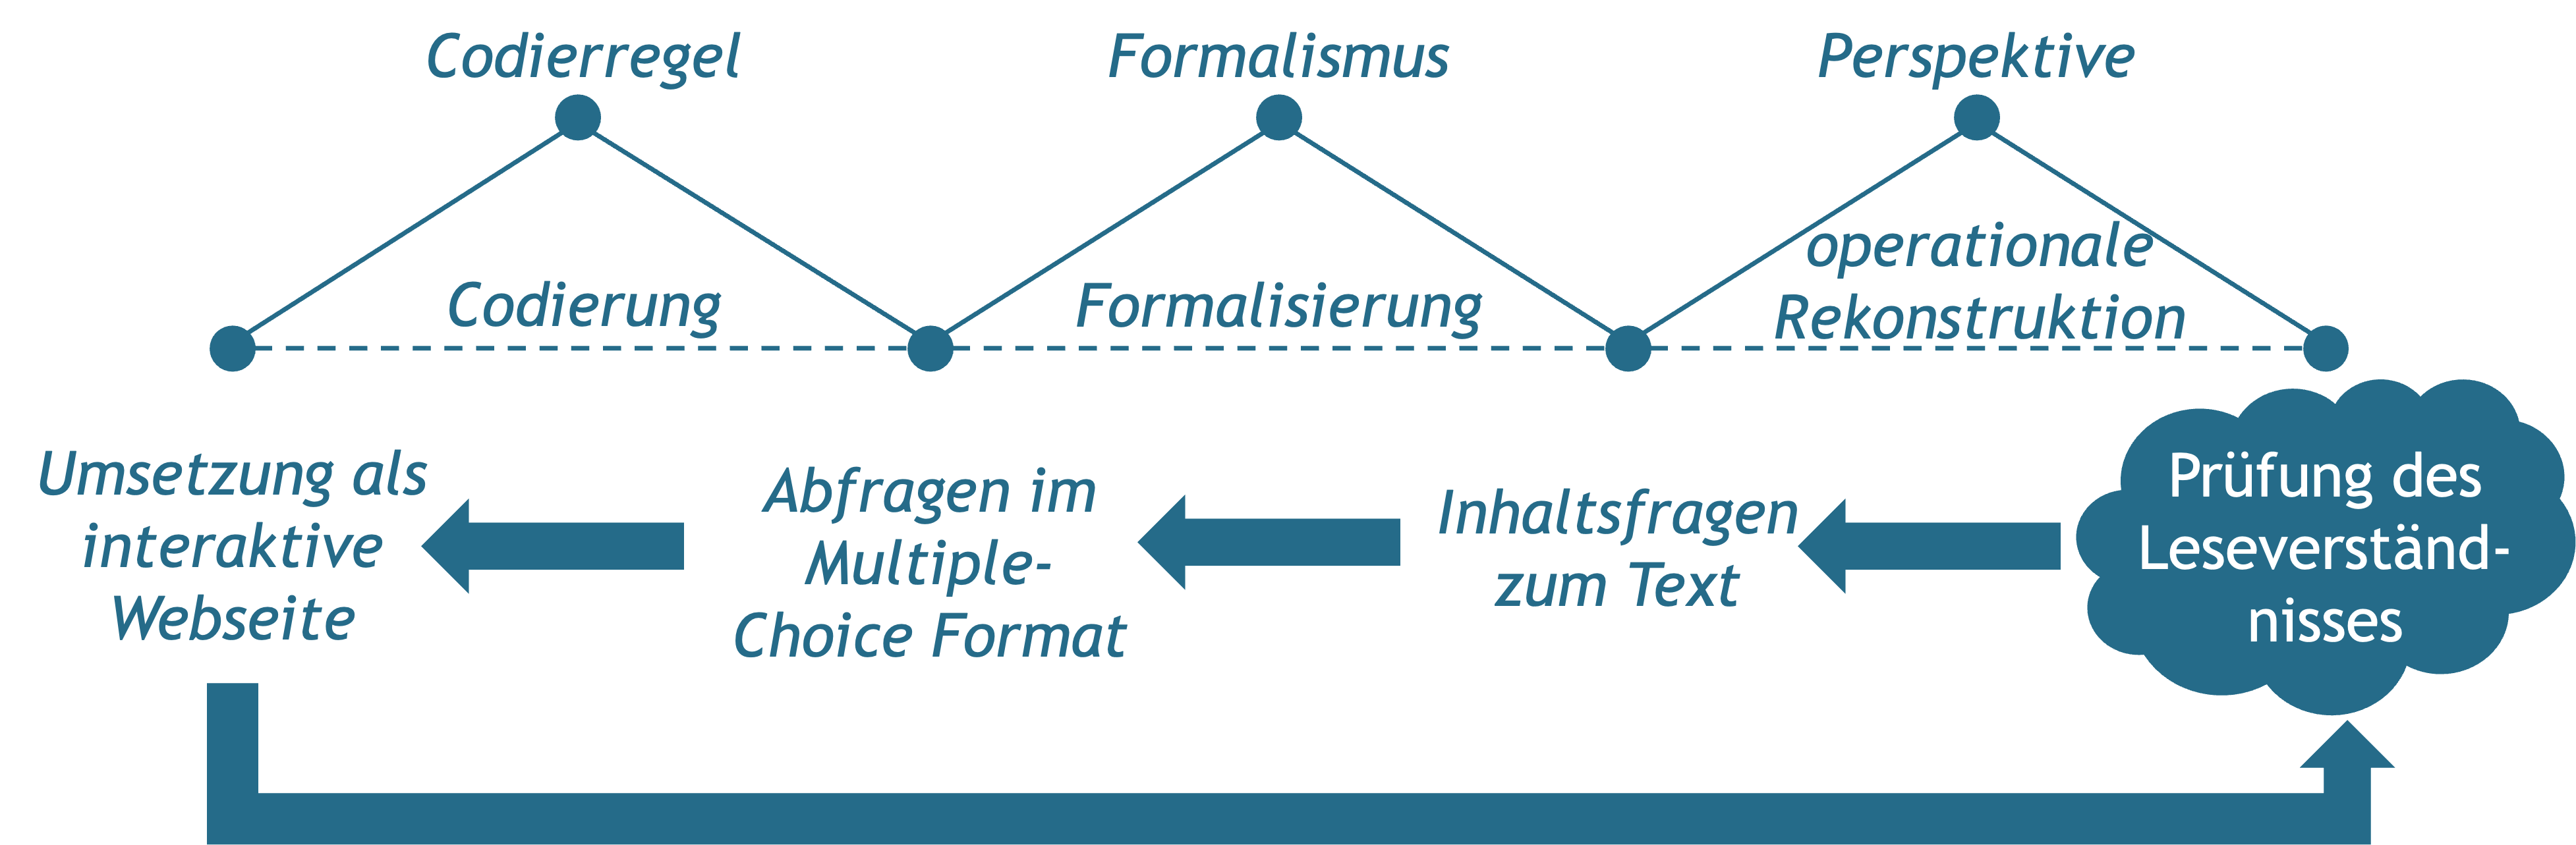
\includegraphics{Figures/09-04-RekonstruktionAntolin} \end{center}

~

\begin{blackbox}
\emph{Von welchen Aspekten des Leseverständnisses wird abstrahiert? Welche neuen Möglichkeiten eröffnen sich?}

\end{blackbox}

\section{Rekonstruktion von Prozessketten}\label{rekonstruktion-von-prozessketten}

\textbf{Ziel}

Die Rekonstruktion von Prozessketten dient dazu, die Schritte eines Vorgangs so zu beschreiben, dass die entsprechenden Prozesse geplant und wiederholt durchgeführt werden können.

\textbf{Leitgedanke}

Die Rekonstruktion von Prozessketten basiert auf der Idee, dass sich wesentliche Aspekte wiederkehrender Prozesse so beschreiben lassen, dass diese Beschreibungen als Anleitungen für andere Menschen aber auch als Grundlage für eine automatisierte Bearbeitung dienen können. Bei der Rekonstruktion werden komplexe Prozesse in einzelne voneinander unterscheidbare Operationen zerlegt, die jeweils durch spezifische Ein- und Ausgaben sowie Bearbeitungsregeln definiert sind. Da entsprechende Modelle von den Details individueller Prozesse abstrahieren, geht mit ihrer Rekonstruktion auch immer eine Unterscheidung von Wesentlichem und Unwesentlichem einher.

\textbf{Anwendungskontext}

Ausgangspunkt für die Rekonstruktion bilden wiederkehrende und regelhaft verlaufende Prozesse. Hierbei kann es sich beispielsweise um routinierte Handlungen, Methoden und Verfahren handeln.

\begin{center}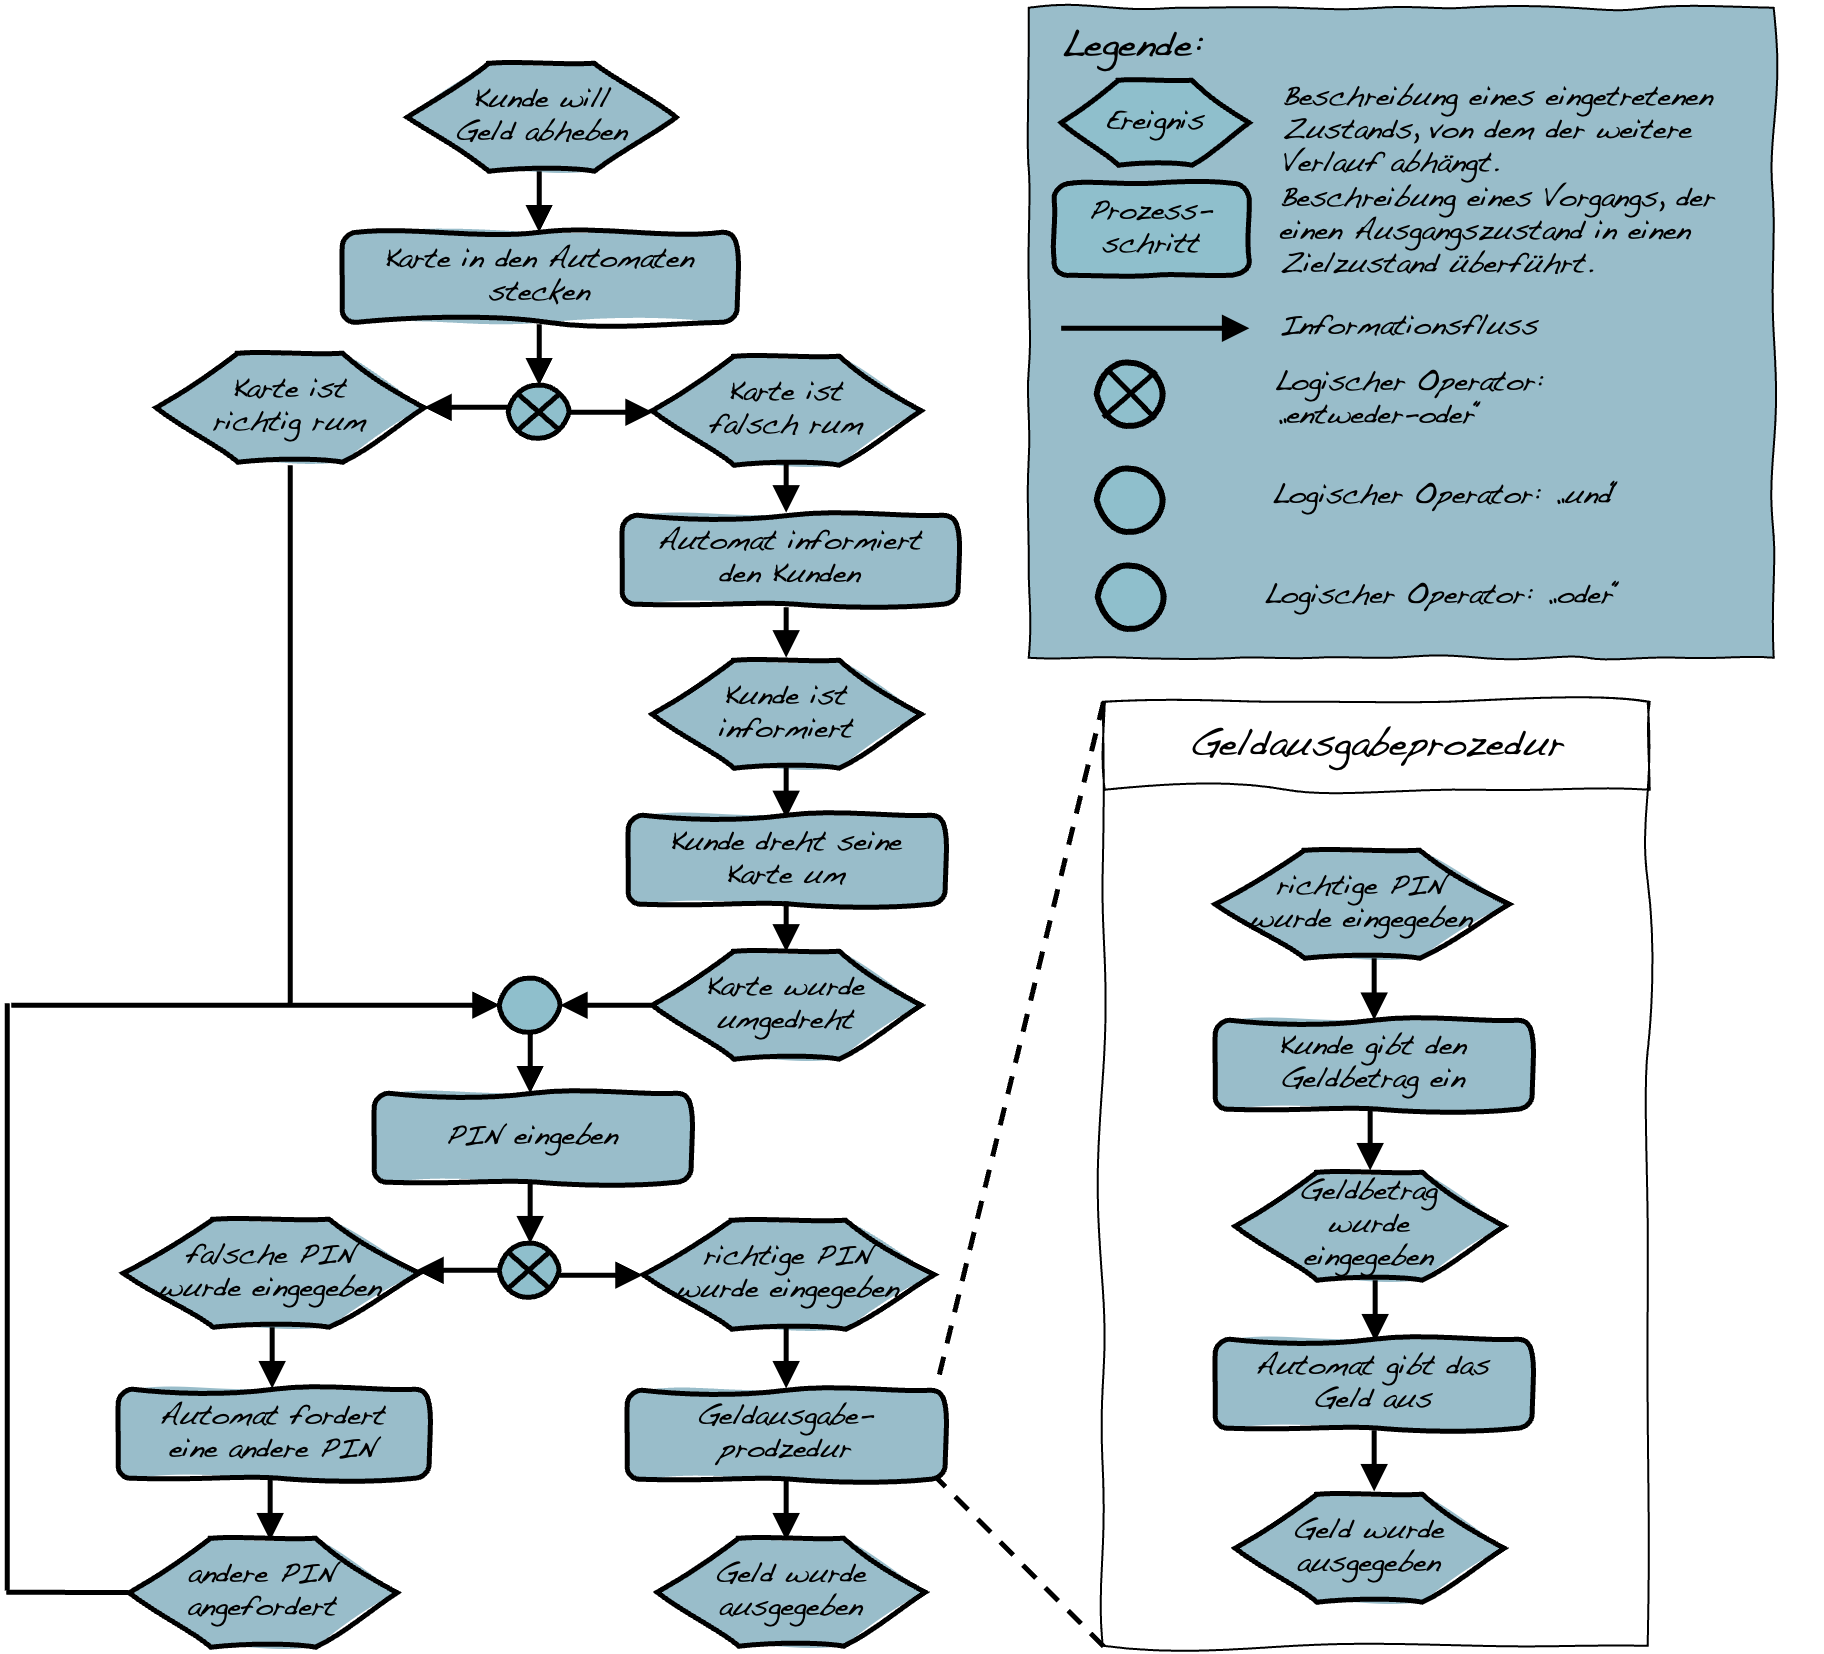
\includegraphics{Figures/09-05-Prozesskette} \end{center}

\textbf{Arbeitsschritte}

\begin{enumerate}
\def\labelenumi{\arabic{enumi}.}
\tightlist
\item
  Auswahl eines wiederkehrenden Handlungsablaufs.
\item
  Sammlung und Sichtung bereits bestehender Beschreibungen des fraglichen Handlungsablaufs (z.B. Anleitungen, Richtlinien, Tutorials).
\item
  Identifikation und Benennung relevanter Ereignisse und Prozesse.
\item
  Organisation und Visualisierung der Ereignisse und Prozesse in einer Prozesskette.
\end{enumerate}

\textbf{Ergebnisformat}

Ein grafische Darstellung als Prozesskette.

\textbf{Praktische Tipps}

\begin{itemize}
\tightlist
\item
  Am Anfang und Ende einer Prozesskette steht jeweils ein Ereignis, das den Ausgangs- beziehungsweise Endzustand beschreibt.
\item
  \textbf{Zwischen zwei Ereignissen liegt immer ein Prozess}, der von einem zum nächsten Ereignis führt.
\item
  Prozesse können sowohl von Menschen wie auch von einem technischen Gerät ausgeführt werden.
\end{itemize}

\textbf{»Fallstricke«}

\begin{itemize}
\tightlist
\item
  Die Rekonstruktion von Prozessketten ist kein Abbildungs-, sondern ein Übersetzungsprozess, der ein kreatives Moment beinhaltet.
\item
  Prozessmodelle lassen sich in unterschiedlichster Form darstellen, wichtig ist, dass alle Elemente definiert sind und konsistent verwendet werden.
\item
  \textbf{Auf ein Ereignis darf keine ›entweder-oder‹-Operation folgen.}
\end{itemize}

\textbf{Weiterführende Literatur zum Leittext}

Floyd, C. (2002). Developing and Embedding Auto-Operational Form. In Y. Dittrich, C. Floyd, \& R. Klischewski (Hrsg.), \emph{Social Thinking---Software Practice} (S. 5--28). MIT Press.

Floyd, C. (1997). Autooperationale Form und situiertes Handeln. \emph{CognitioHumana- XVII. Deutscher Kongreß für Philosophie}, 237
252. \url{https://doi.org/10.1515/9783050073651}

Keller, G., Nüttgens, M., \& Scheer, A.-W. (1992). \emph{Semantische Prozeßmodellierung auf der Grundlage »Ereignisgesteuerter Prozeßketten (EPK)}« (Nr. 89; Veröffentlichungen des Instituts für Wirtschaftsinformatik (IWi)). Universität des Saarlandes. \url{https://web.archive.org/web/20190109111105/http://www.unisaarland.de/fileadmin/user_upload/Fachrichtungen/fr13_BWL/professuren/PDF/heft89.pdf}

\chapter{Daten und Informatisierung}\label{daten-und-informatisierung}

Die automatisierte Ausführung und Steuerung praktisch relevanter Vorgänge mittels digitaler Technologien setzt neben der operationalen Rekonstruktion von Prozessen immer auch die \textbf{Übersetzung relevanter Phänomene in Daten} voraus. Das, was in einem bestimmten Gegenstandsbereich als relevant erachtet wird, muss zunächst in Form von Daten verfügbar gemacht werden, bevor es von einem Programm verarbeitet werden kann.

»In solving a problem with or without a computer it is necessary to choose an abstraction of reality, i.e., to define a set of data that is to represent the real situation. This choice must be guided by the problem to be solved.« \citep{wirthAlgorithmsDataStructures1976}

\begin{figure}

{\centering 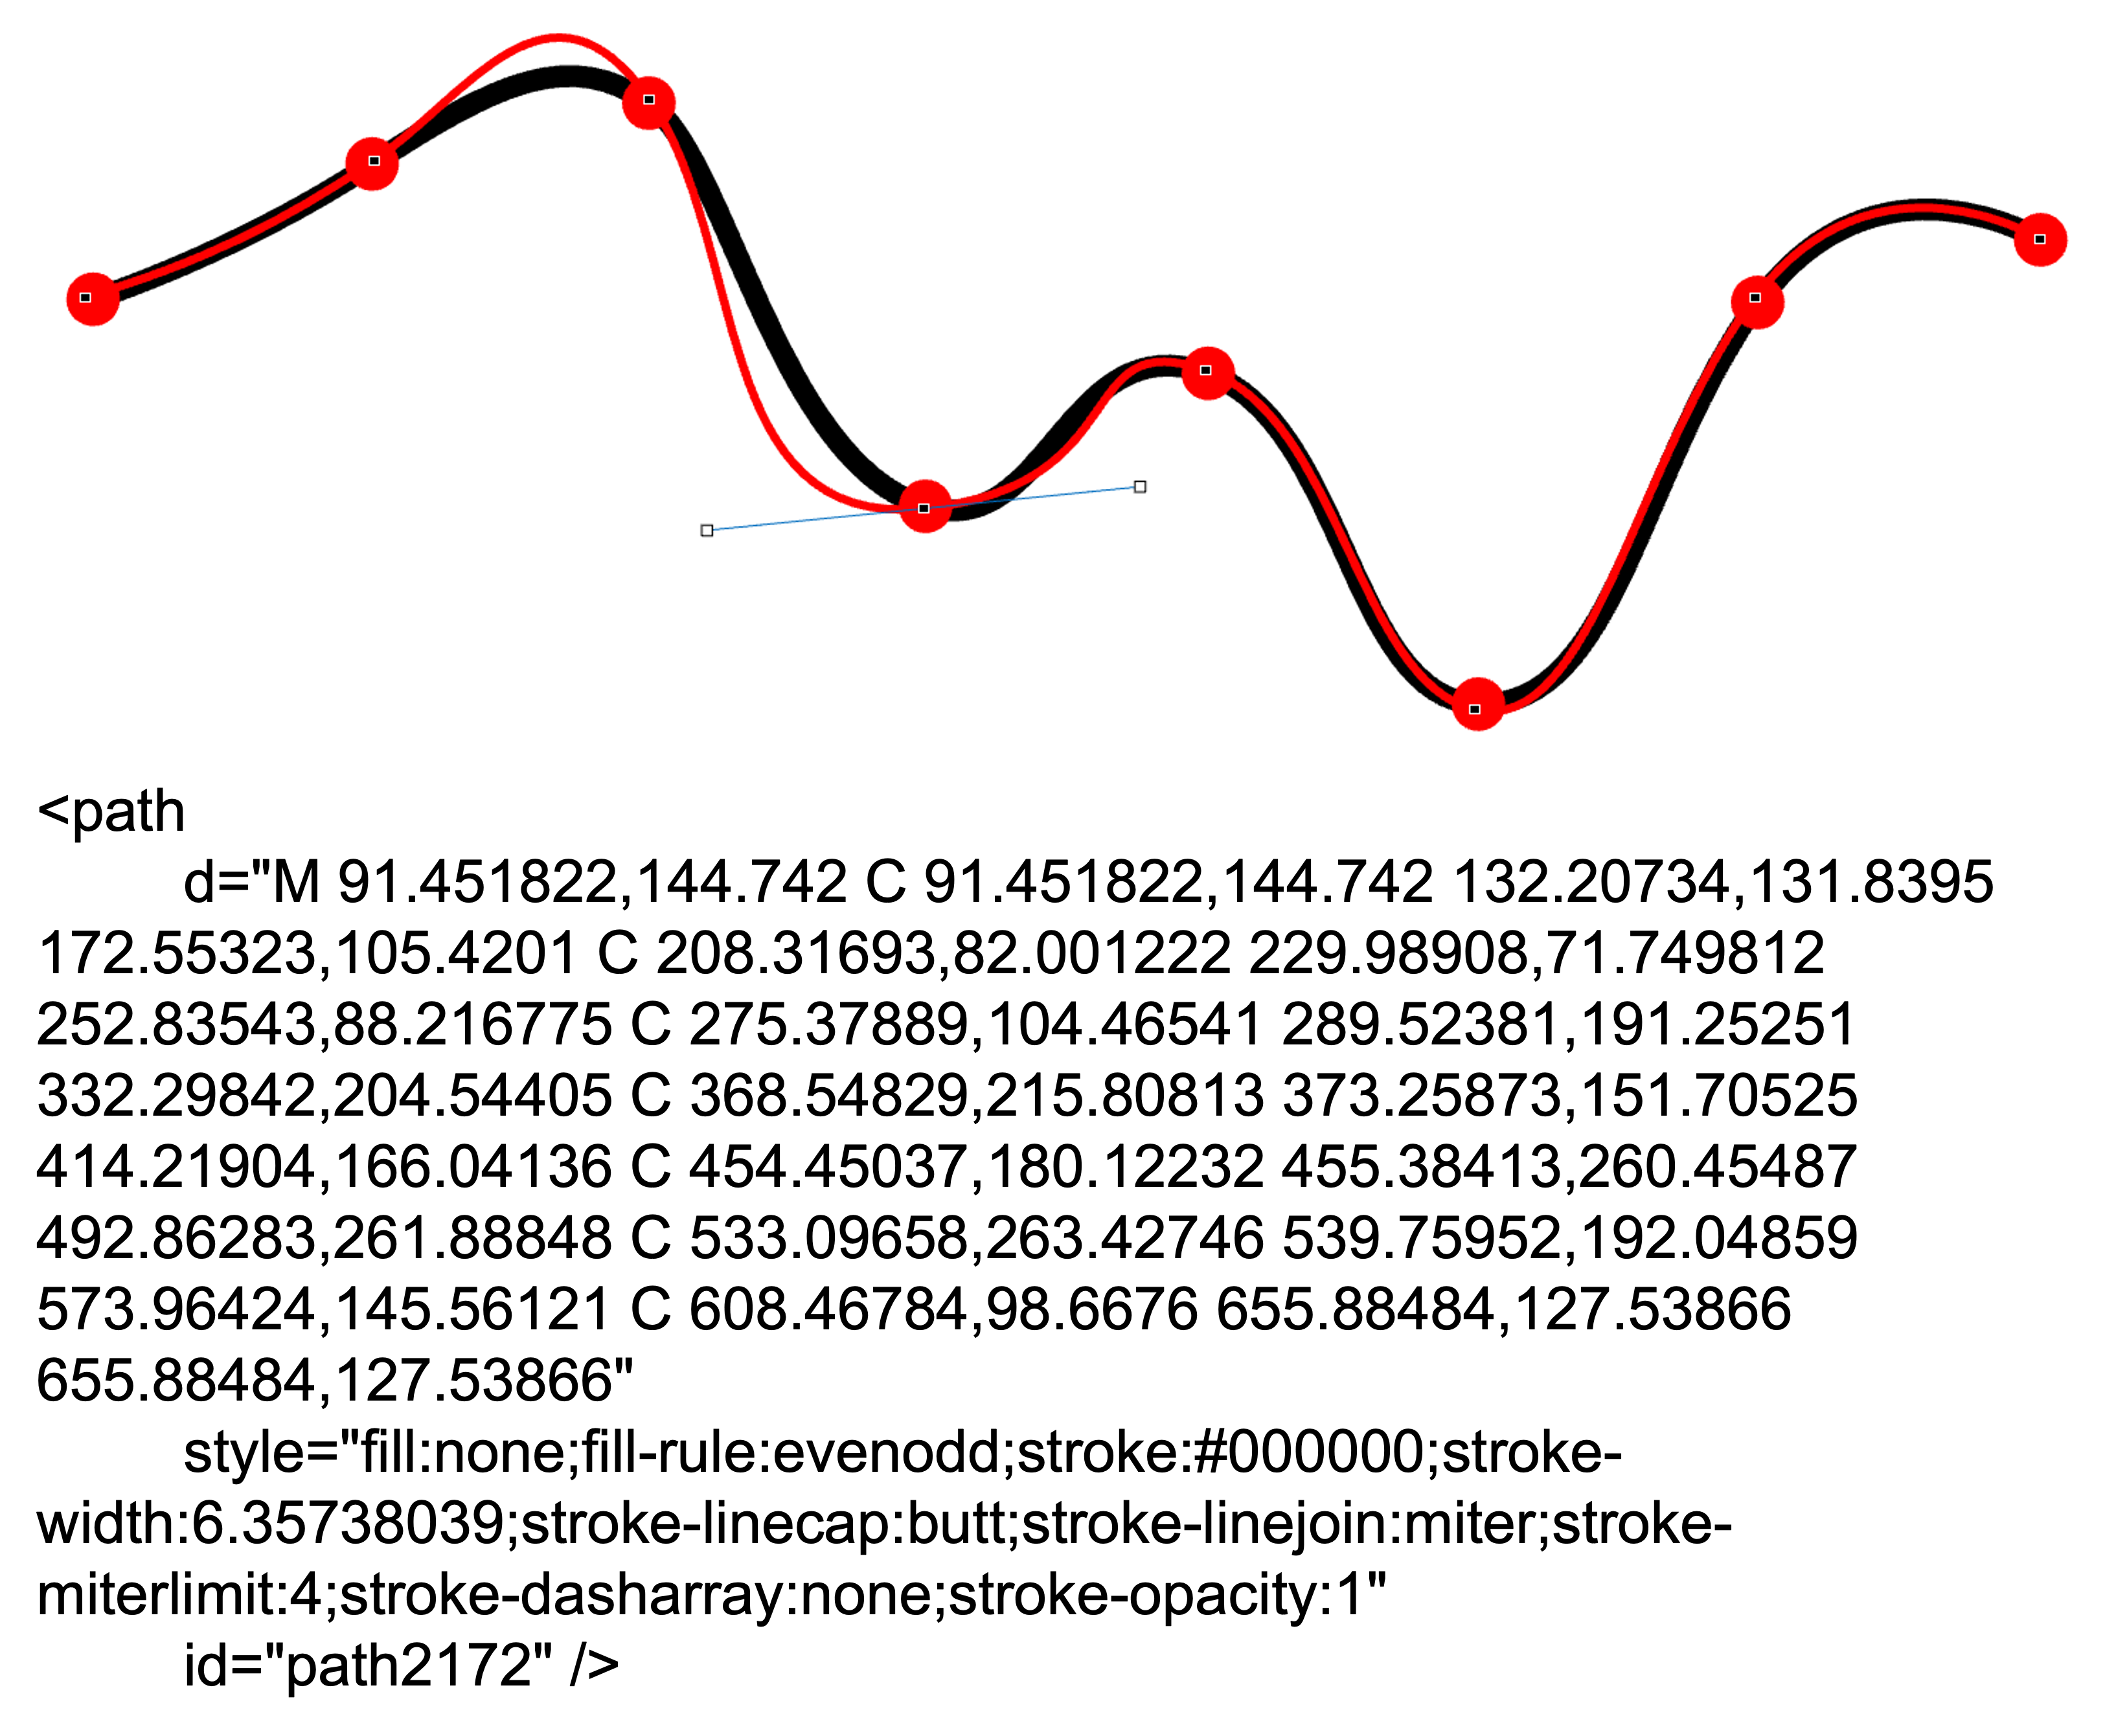
\includegraphics{Figures/10-01} 

}

\caption{Die Übersetzung eines Linienzugs in ein digitales Datenobjekt.}\label{fig:fig15}
\end{figure}

\section{Die Datafizierung des Gegenstandsbereich als Voraussetzung der Digitalisierung}\label{die-datafizierung-des-gegenstandsbereich-als-voraussetzung-der-digitalisierung}

Informationen können nur dann von digitalen Technologien verarbeitet werden, wenn sie in Form eindeutig bestimmter Daten vorliegen. Daten können dabei aus informatischer Sicht als eine \textbf{»reinterpretable representation of information in a formalized manner suitable for communication, interpretation, or processing«} \citep{iec23822015InformationTechnologyVocabulary2015} verstanden werden, die in diskreten Datenobjekten organisiert sind.

Entgegen der etymologischen Bedeutung des Wortes Datum als dem \textbf{Gegebenem}, sind Daten im informationstechnischen Sinne vielmehr etwas \emph{Gemachtes}. Sie werden in einer Weise erzeugt, die für die automatisierte Kommunikation, Interpretation und Verarbeitung geeignet ist. Damit dies möglich wird, muss ihre Verarbeitung \textbf{vollkommen unabhängig von der Interpretation durch einen Menschen} sein \citep[vgl.][]{nakeAlgorithmischeZeichen2001} . Daten existieren dementsprechend nicht nur an und für sich, sondern müssen mit Hilfe entsprechender praktischer Vorkehrungen und Instrumente erzeugt werden \citep[vgl. z.B.][]{gitelmanIntroduction2013, giessmannWasIstDatenkritik2014}. Da analoge, kontinuierliche Ereignisse zum Zweck der digitalen Verarbeitung in diskrete Datenobjekte überführt werden müssen, impliziert die Generierung immer auch den Rückgriff auf entsprechende Datenmodelle und eine hiermit einhergehende explizite oder implizite Kategorisierung. Die Entwicklung digitaler Technologien bedingt insofern immer auch eine \textbf{»Informatisierung des Gegenstandsbereichs«} \citep[S. 245]{floydAutooperationaleFormUnd1997}. Alles, was sich nicht in Daten überführen lässt, entzieht sich somit der digitalen Verarbeitung.

Parallel zum Prozess des Programmierens lässt sich auch die ›Datafizierung‹ als ein \textbf{mehrstufiger Vorgang} verstehen (siehe {Abb. 10.2}). Hierbei wird zunächst ein Gegenstand im Anwendungsbereich mittels einer Sammlung relevanter Informationen überführt, die dann in eine formale Datenstruktur und schließlich in ein digitales Datenobjekt übersetzt werden.

\begin{figure}

{\centering \includegraphics{Figures/10-02-Übersetzung} 

}

\caption{Datafizierung als ein mehrstufiger Übersetzungsprozess.}\label{fig:fig16}
\end{figure}

\section{Wesentliche Ideen}\label{wesentliche-ideen-2}

\textbf{(Digitale) Daten sind Zeichen, die Informationen darstellen -} Daten repräsentieren Informationen über einen Gegenstand. Sie sind eine Form der Beschreibung, die zu einem bestimmten Zweck vorgenommen wird. Damit Daten automatisiert verarbeitet werden können, müssen sie formalisiert werden, sodass ihre Bedeutung eindeutig definiert ist. Im Sinne einer Beschreibung sind Daten nicht gegeben, sondern gemacht. Daten sind insofern niemals ›roh‹ (d.h. unverarbeitet) und können strenggenommen als solche auch nicht gesammelt oder erfasst werden \citep[vgl.][]{gitelmanIntroduction2013}.

\textbf{Die Produktion (digitaler) Daten kann selbst in unterschiedlichem Maße automatisiert sein -} (Digitale) Daten können auf unterschiedliche Weise produziert werden. Neben der direkten und gezielten Eingabe durch einen Menschen (z.B. beim Ausfüllen eines Formulars am Bildschirm), können Daten auch durch automatisierte Messgeräte (z.B. Thermometer, GPS, Bewegungssensoren, \ldots) erzeugt werden. Darüber hinaus können digitale Daten auch in der unmittelbaren Interaktion mit einem digitalen Produkt automatisch generiert werden (z.B. Logfile- und Interaktionsdaten). Je nach Art und Weise der Datenproduktion verlagern sich die Kontrollmöglichkeiten für die Anwender*innen.

\textbf{Als Beschreibungen sind Daten reduktiv -} Wie alle anderen sprachlichen Beschreibungsformate sind auch Daten reduktiv, da sie von der Komplexität realweltlicher Phänomene abstrahieren und entsprechend der jeweiligen Zwecksetzung Wesentliches von Unwesentlichem trennen \citep[vgl.][]{floydAutooperationaleFormUnd1997, nakeAlgorithmischeZeichen2001}. Als Beschreibungen abstrahieren Daten insbesondere von der Einzigartigkeit und Überschüssigkeit der Dinge und fokussieren die Gemeinsamkeiten und Beziehungen zwischen den Dingen, die bereits bekannt sind (und sich in Daten fassen lassen).

\textbf{Daten sind aggegrativ -} Daten erlangen ihre Aussagekraft durch den Vergleich und die Bezugnahme auf andere Daten. Als Datenobjekte haben sie zwar einen eigenständigen Charakter, bedeutsam werden sie aber erst in Relation zu anderen Daten (z.B. steht ein geschichtliches Datum in einem chronologischen Verhältnis zu anderen Daten). Die Produktion von Daten ist dementsprechend ein auf Systematisierung und Akkumulation ausgerichteter Prozess. Daten sind somit immer auch Teil umfassender Datensammlungen \citep[vgl.][]{giessmannWasIstDatenkritik2014}.

\textbf{Die systematische Nutzung von Daten erfordert die Entwicklung von Kategorien und standardisierter Datenformate -} Sobald Daten gesammelt und aggregiert werden, bedarf es definierter Kategorien und standardisierter Datenformate, damit Daten verglichen und ausgetauscht werden können. Entsprechende Kategorien legen zum Beispiel fest, welche Merkmalsausprägungen einer zu beschreibenden Eigenschaft unterschieden werden sollen und wie die einzelnen Merkmalsausprägungen definiert sind. Datenformate wiederum regeln, wie die Daten codiert werden, sodass sie in automatisierter Weise verarbeitet werden können.

\textbf{Als digitale Datenobjekte intervenieren Daten in die Gegenstandsbereiche, die sie zu repräsentieren vorgeben -} Als Objekte sind Daten selbst Gegenstand sozialer Praktiken. Insofern sich in hochgradig technisierten Gesellschaften viele Phänomene erst durch komplexe Datensammlungen erschließen oder selbst das Produkt digitaler Technologien sind, haben Daten nicht nur eine repräsentierende, sondern auch eine wirklichkeitskonstitutierende Funktion. Daten werden insofern zunehmend zu einem Bezugspunkt, an dem Individuen wie auch soziale Gruppen ihr Handeln orientieren.

\section{Beispiel und Diskussionspunkt -- Die Datafizierung von Lernprozessen in Lernmanagementsystemen}\label{beispiel-und-diskussionspunkt-die-datafizierung-von-lernprozessen-in-lernmanagementsystemen}

Mit der zunehmenden Verbreitung digitaler Technologien ist auch das Interesse an der Dokumentation und Analyse von Lernprozessen gestiegen. Digitale Schulbücher, Anwendungen und Lernmanagementsysteme stellen in vielen Fällen nicht mehr nur Inhalte oder Lernangebote zur Verfügung, sondern dokumentieren auch das Interaktionsverhalten der Lernenden. Anhand der gesammelten Daten können sich, je nach Konfiguration der Anwendung, die Lehrer*innen, Eltern, und/oder Schüler*innen über ihre Aktivitäten wie auch die jeweiligen Lernfortschritte informieren.

Die Datafizierung von Lernprozessen lässt sich, wie im Folgenden am Beispiel eines Lernmanagementsystems dargestellt, als eine Reihe von Übersetzungsschritten auffassen.

\begin{center}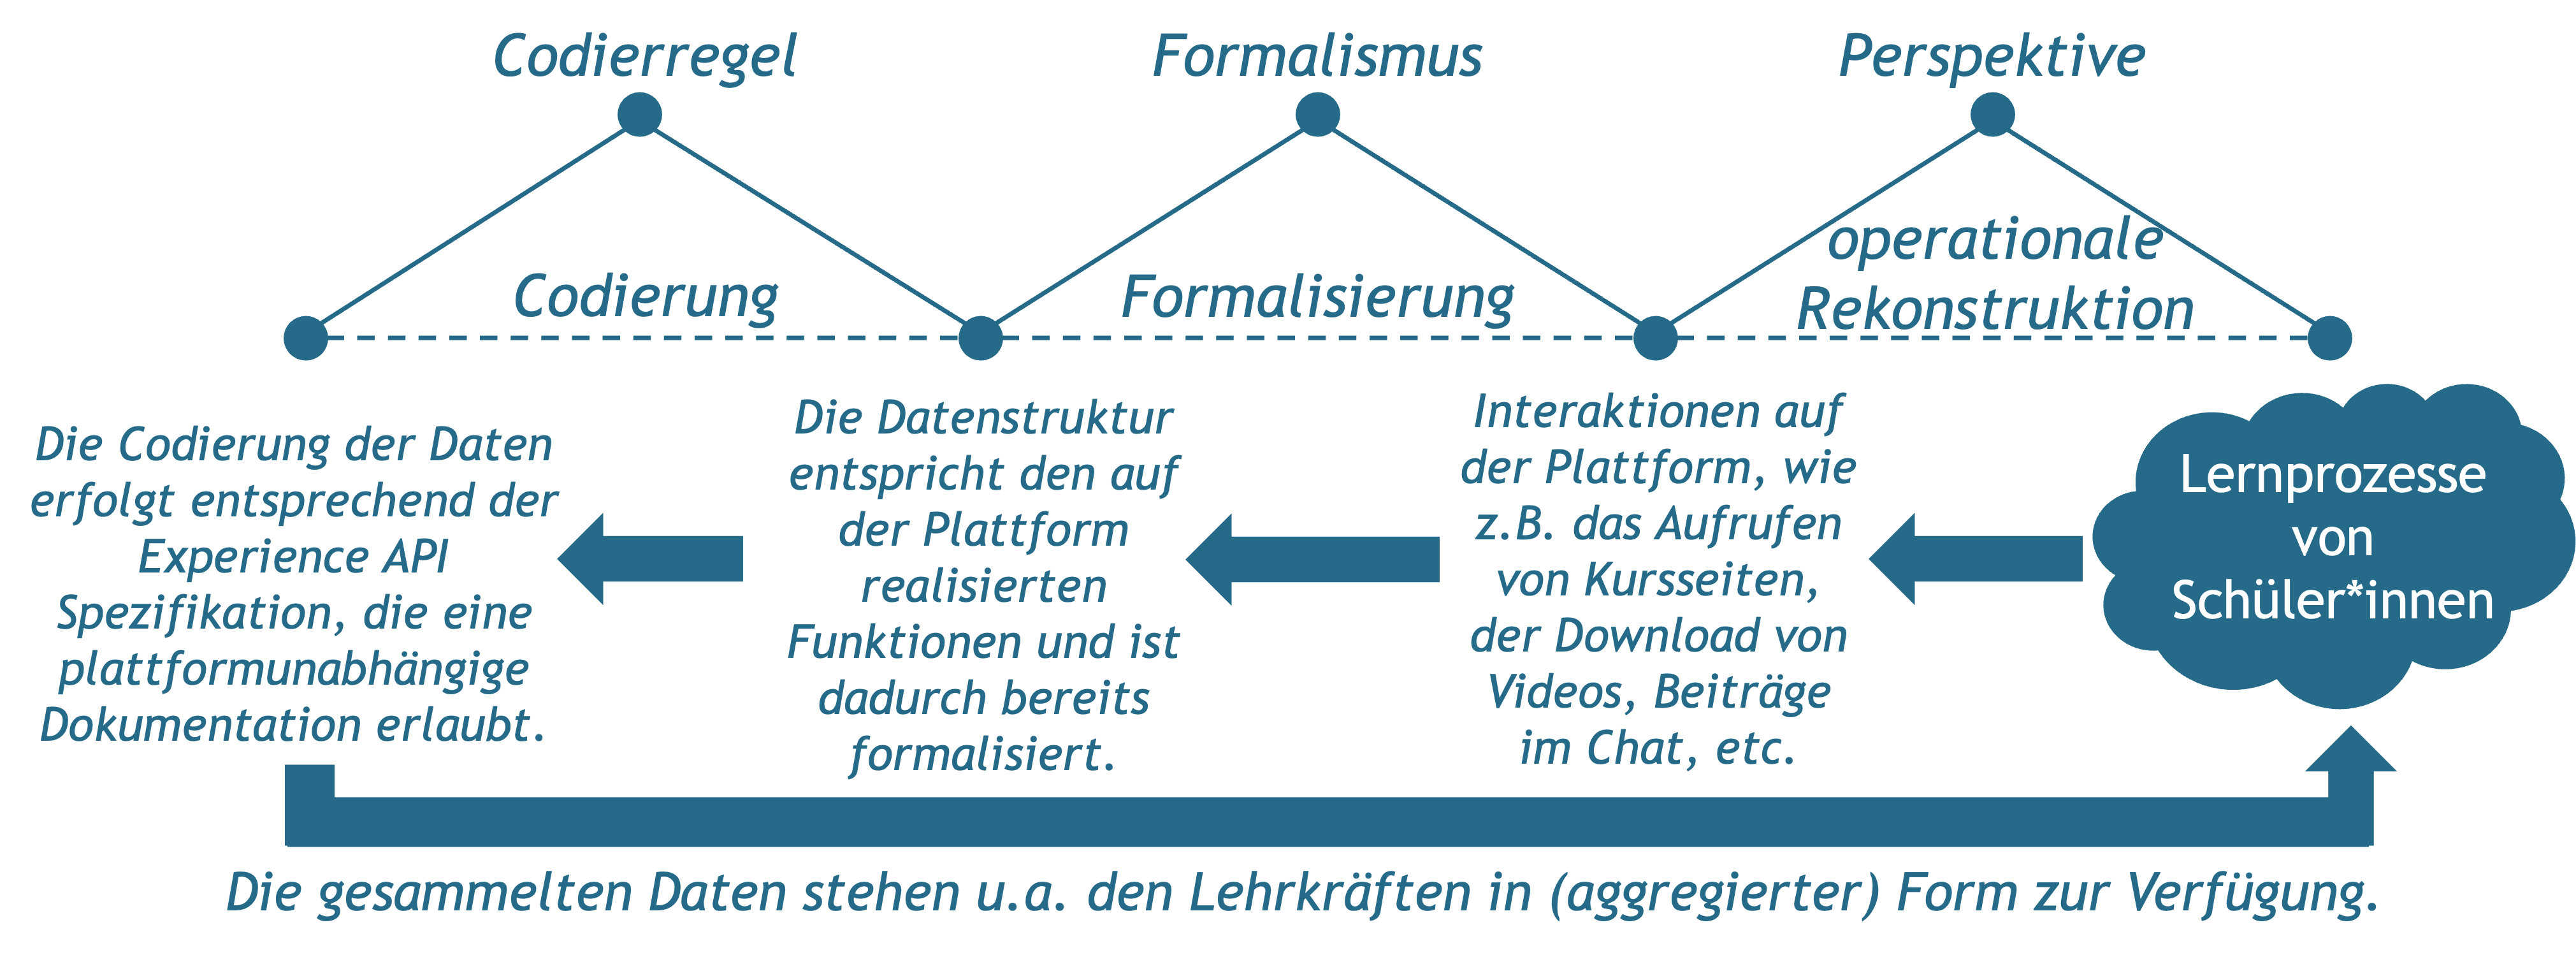
\includegraphics{Figures/10-04-Lernmanagementsystem} \end{center}

~

\begin{blackbox}
\emph{Welche Aspekte des Lernens finden durch die verschiedenen Übersetzungen besondere Beachtung und welche werden nicht erfasst beziehungsweise ausgeblendet?}

\end{blackbox}

\section{Anwendungsbezogene Datenkritik}\label{anwendungsbezogene-datenkritik}

\textbf{Ziel}

Ziel der anwendungsbezogenen Datenkritik ist es, die mit der Produktion von Daten einhergehenden Übersetzungen nachzuzeichnen und den Einfluss der Datafizierung auf den Gegenstandsbereich zu reflektieren.

\textbf{Leitgedanke}

Die anwendungsbezogene Datenkritik basiert auf der Idee, dass wesentliche Aspekte eines Gegenstandsbereichs in Daten übersetzt werden müssen, damit sie von digitalen Technologien verarbeitet werden können. Diese ›Informatisierung des Gegenstandsbereichs‹ (Floyd, 1997) lässt sich als ein mehrstufiger und zweckgebundener Prozess verstehen, durch den spezifische Weltzugänge produziert werden. Da Daten von der Komplexität des Gegenstandsbereichs abstrahieren, liegt ihrer Verwendung auch immer eine Unterscheidung von Wesentlichem und Unwesentlichem zugrunde.

\textbf{Anwendungskontext}

Ausgangspunkt für die Datenkritik bilden die in einem bestimmten Anwendungskontext generierten und mittels digitaler Technologien verarbeiteten Daten.

\begin{center}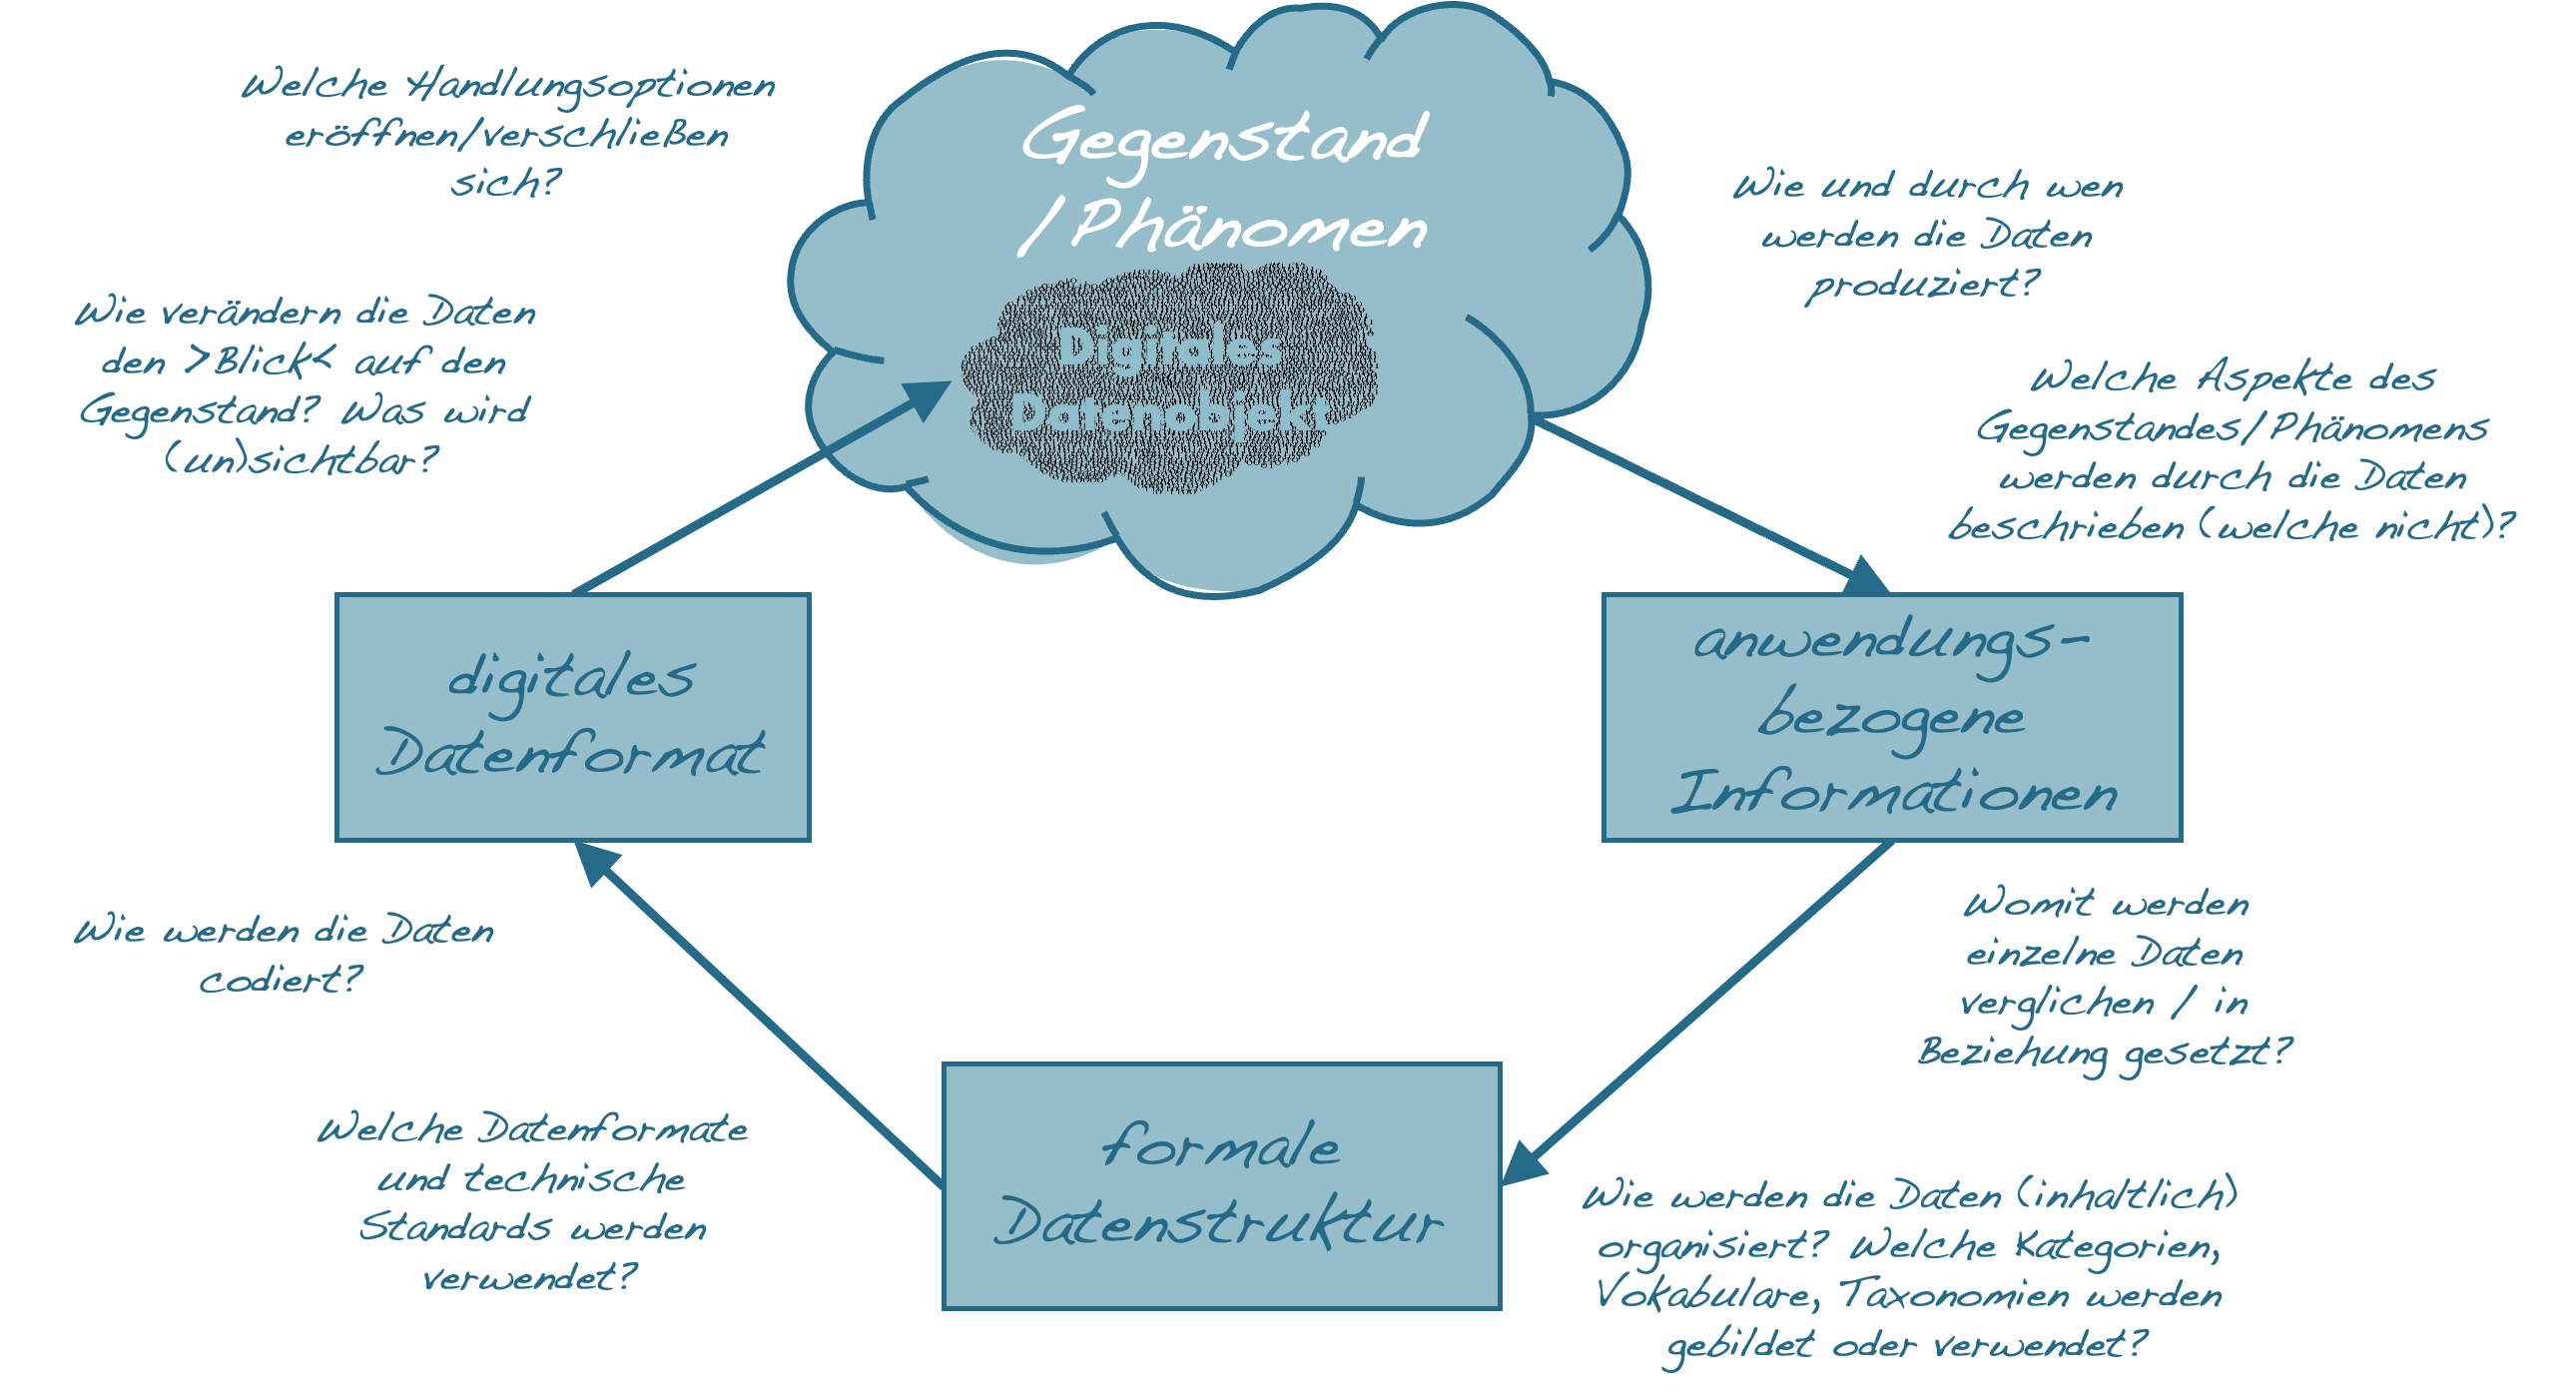
\includegraphics{Figures/10-05-anwendungsbezogeneDatenkritik} \end{center}

\textbf{Arbeitsschritte}

\begin{enumerate}
\def\labelenumi{\arabic{enumi}.}
\tightlist
\item
  Identifikation der für eine Anwendung relevanten digitalen Daten.
\item
  Identifikation des durch die Daten dargestellten Gegenstandes/Phänomens.
\item
  Rekonstruktion der zugrundeliegenden Übersetzungsschritte.
\item
  Analyse impliziter Annahmen und Verzerrungen.
\end{enumerate}

\textbf{Ergebnisformat}

Erläuterte Illustration grundlegender Übersetzungsschritte.

\textbf{Praktische Tipps}

\begin{itemize}
\tightlist
\item
  Jeder Übersetzungsschritt basiert auf einer Perspektive anhand derer zwischen Wesentlichem und Unwesentlichem unterschieden wird.
\item
  Zum besseren Verständnis bietet es sich an, die einzelnen Übersetzungsschritte anhand eines Beispiels zu illustrieren.
\end{itemize}

\textbf{»Fallstricke«}

\begin{itemize}
\tightlist
\item
  Die anwendungsbezogene Datenkritik ist kein Abbildungs-, sondern selbst ein Übersetzungsprozess, der ein kreatives Moment beinhaltet.
\item
  Gerade dann, wenn Daten als gegeben und ihre Verwendung als alternativlos erscheint, sollte dies die Aufmerksamkeit wecken.
\end{itemize}

\textbf{Weiterführende Literatur zum Leittext}

Dander, V. (2014). Von der ‹Macht der Daten› zur ‹Gemachtheit von Daten›. Praktische Datenkritik als Gegenstand der Medienpädagogik. \emph{Mediale Kontrolle unter Beobachtung}, 3(1), 0--21.

Floyd, C. (1997). Autooperationale Form und situiertes Handeln. \emph{CognitioHumana - XVII. Deutscher Kongreß für Philosophie}, 237--252. \url{https://doi.org/10.1515/9783050073651}

\chapter{Schnittstellen}\label{schnittstellen}

Digitale Technologien sind neben den in ihnen realisierten Algorithmen und Datenstrukturen auch durch die Schnittstellen zu ihrer Umgebung definiert. Diese \textbf{Schnittstellen} umfassen sowohl \textbf{technische Schnittstellen}, über die eine Verbindung und ein Austausch zu anderen technischen Dingen möglich wird, wie auch die \textbf{Benutzungsschnittstellen}, durch die Mensch und Maschine miteinander interagieren.

Benutzungsschnittstellen bestimmen die Möglichkeiten der Mensch-Maschine-Interaktion und sind die Voraussetzung einer praktischen »Kopplung zwischen Mensch und Computer« \citep[S. 4]{herczegSoftwareergonomie2005}.

\begin{figure}

{\centering 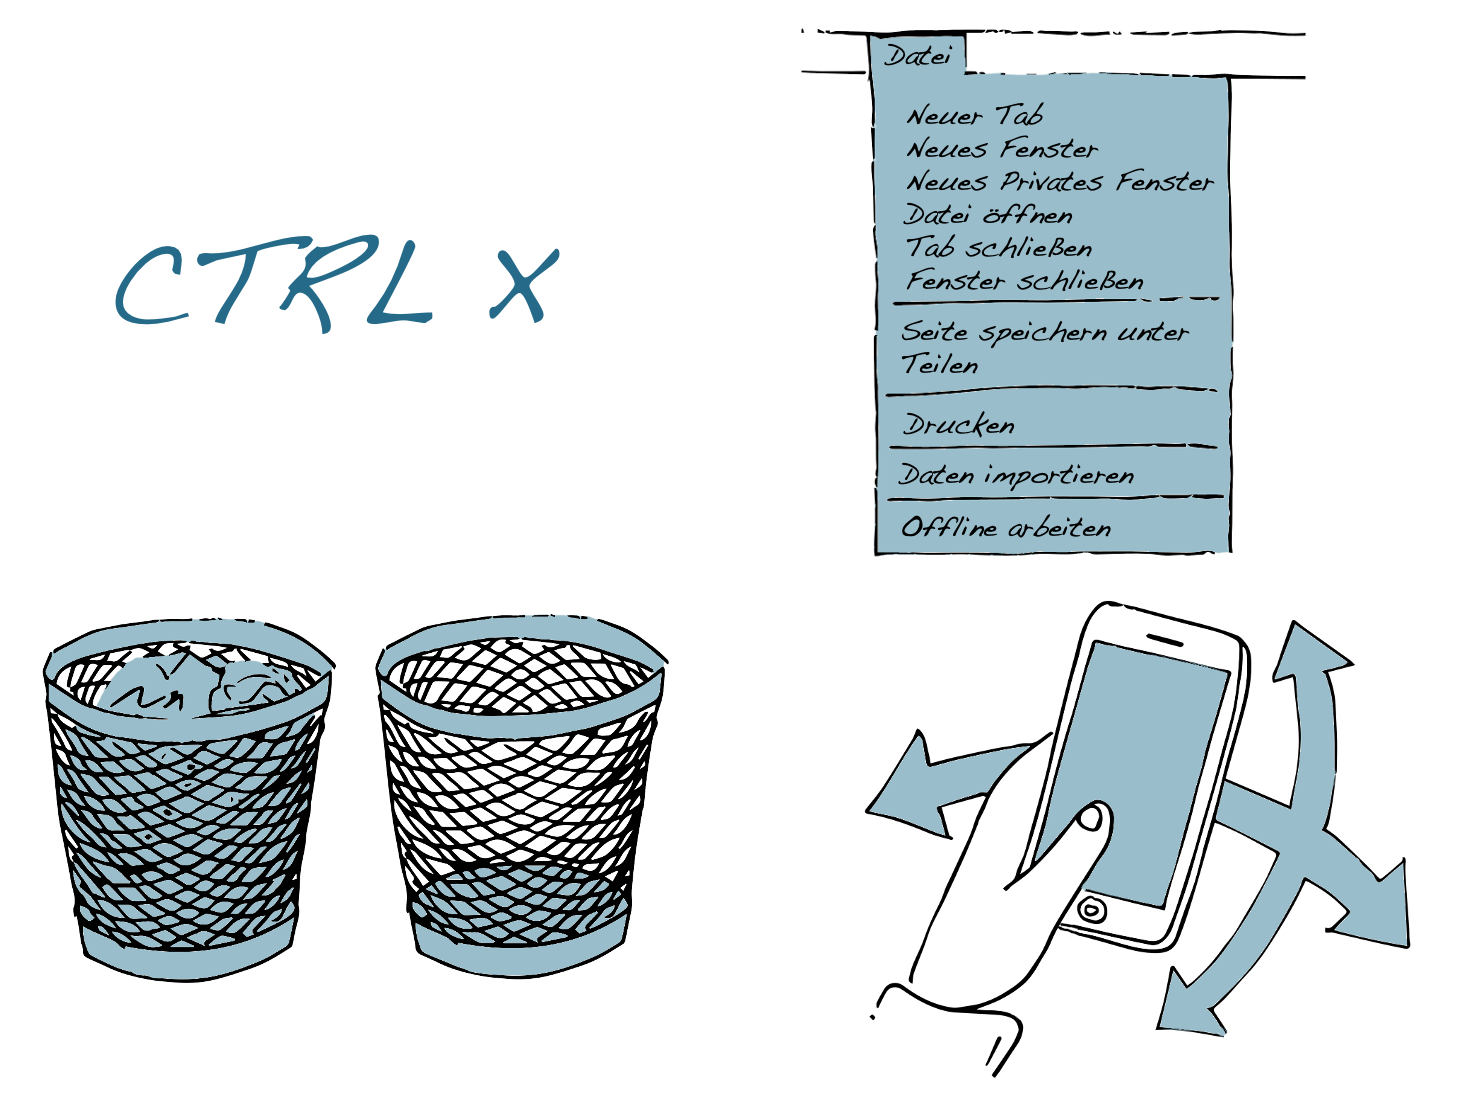
\includegraphics{Figures/11-01-Schnittstellen} 

}

\caption{Beispiele unterschiedlicher Interaktionsformen; vom Befehl über Menüs und grafischen Benutzungsoberflächen zu Gesten.}\label{fig:fig17}
\end{figure}

\section{Die Einbindung der digitalen Dinge in ihre Umgebung}\label{die-einbindung-der-digitalen-dinge-in-ihre-umgebung}

Damit digitale Dinge, wie etwa ein Textverarbeitungsprogramm, eine Anwendung zur Aufnahme von Fotos mit dem Smartphone oder auch eine Messenger-App, ›funktionieren‹ können, müssen sie sowohl \textbf{in ihre technische wie auch nicht-technische Umgebung eingebunden} sein. Hierzu bedarf es vielfältiger \textbf{Schnittstellen (Interfaces)}, die eine Verbindung zwischen den verschiedenen digitalen Dingen, aber auch zwischen den digitalen Dingen und ihren Anwender*innen herstellen.

Eine Schnittstelle lässt sich dabei sehr allgemein als eine \textbf{gemeinsame Grenze zwischen zwei funktionalen Einheiten} verstehen, die durch eindeutig definierte Funktionen, physische Verbindungen oder Formate zum Informationsaustausch charakterisiert ist \citep[vgl.][]{iec23822015InformationTechnologyVocabulary2015}. Schnittstellen ermöglichen die Interaktion bzw. Kommunikation zwischen unterschiedlichen Dingen. Durch die eindeutige Definition der Schnittstelle wird die Interaktion bzw. Kommunikation über die gemeinsame Grenze hinweg möglich, ohne dass die hieran beteiligten Dinge oder Akteur*innen wissen müssen, wie eine bestimmte Funktion auf der anderen Seite der Grenze realisiert ist oder wie die übermittelten Informationen dort konkret verarbeitet werden. Voraussetzung für eine funktionierende Schnittstelle ist vielmehr die ›Passfähigkeit‹ der durch die Schnittstelle verbundenen Dinge.

Neben \textbf{Hardwareschnittstellen}, über die verschiedene Geräte physisch miteinander verbunden werden (z.B. USB-Anschluss), regeln \textbf{Softwareschnittstellen} den Austausch von Daten und die Synchronisation bzw. Steuerung von Prozessen zwischen unterschiedlichen Programmen oder Programmkomponenten. Die sogenannten \textbf{Benutzungsschnittstellen} (user interfaces) markieren wiederum die Grenze, bzw. die Punkte, eines technischen Gerätes, an denen menschliche Akteur*innen mit diesem interagieren. Auch die Benutzungsschnittstellen können sowohl hardware- (z.B. Maus, Touchscreen, Mikrofon) wie auch softwaretechnisch (z.B. virtueller Desktop) realisiert sein. Benutzungsschnittstellen umfassen sowohl \textbf{Eingabe-} (z.B. per Tastatur, Gesten, Sprache, etc.) wie auch \textbf{Ausgabemöglichkeiten} (z.B. per Bildschirm, Lautsprecher, Drucker etc.), mittels derer menschliche Akteur*innen mit einer digitalen Technologie interagieren können.

\begin{figure}

{\centering 
\includegraphics[width=0.5\linewidth]{Figures/11-02-Karl-Klammer} 

}

\caption{ Der digitale Assistent ›Karl Klammer‹ in Microsoft Office 2000.}\label{fig:fig18}
\end{figure}

\section{Formen der Mensch-Maschine-Interaktion}\label{formen-der-mensch-maschine-interaktion}

Im Unterschied zu anderen Schnittstellen lässt sich bei Benutzungsschnittstellen nur die technische Seite formal festlegen. Die menschliche Seite bleibt zumindest in Teilen unbestimmt; unerwartetes und spontanes Verhalten ist möglich. Zudem ist der Umgang mit technischen Dingen immer auch von den individuellen Erfahrungen und Erwartungen der Anwender*innen geprägt, die nur bedingt den tatsächlich realisierten technischen Bedingungen entsprechen müssen. Eine zentrale Herausforderung bei der Gestaltung besteht deshalb darin, Interaktionsformen zu finden, die die technischen Gegebenheiten mit den Gewohnheiten und Erwartungen der Anwender*innen in Einklang bringen.

Im Laufe der Zeit sind verschiedene Formen der Mensch-Maschine-Interaktion entwickelt worden. Das Spektrum reicht von der Interaktion durch \textbf{›Befehle‹}, über die \textbf{menübasierte Steuerung} von Programmen und \textbf{grafische Benutzeroberflächen}, in denen Interaktionselemente bildlich dargestellt und z.B. mittels einer Maus bedient werden, bis hin zur Steuerung digitaler Technologien durch \textbf{Sprache, Gesten oder der direkten Manipulation der physischen Umwelt}, etwa mittels gegenständlicher Benutzungsschnittstellen (tangible user interfaces). Die Benutzungsschnittstellen setzen dabei jeweils ein entsprechendes Vorwissen der Anwender*innen voraus. Während Befehle explizit gelernt werden müssen, erfordern sowohl grafische wie auch gegenständliche Benutzungsschnittstellen oft ein praktisches Erfahrungswissen \citep[vgl. z.B.][]{schelhoweTechnologieImaginationUnd2007}. Einen Grenzfall bilden sogenannte \textbf{unsichtbare Benutzungsschnittstellen}, die keine bewusste Interaktion voraussetzen, sondern vielmehr menschliches Verhalten automatisiert registrieren und auf dieses eigenständig reagieren, wie etwa bei automatischen Türöffnern oder Schrittzählern im Smartphone.

Ebenso vielfältig wie die Formen der Eingabe sind auch die Ausgabemöglichkeiten, mittels derer die Anwender*innen über den jeweiligen Zustand des digitalen Systems und die verfügbaren Handlungsoptionen informiert werden. Die Möglichkeiten reichen hierbei von optischen, akustischen oder taktilen \textbf{Hinweisreizen} über die Ausgabe von \textbf{Fehlermeldungen} und spezifischen \textbf{Eingabeaufforderungen} bis zur \textbf{Sperrung bestimmter Funktionen}.

Die Ausgestaltung der Benutzungsschnittstelle impliziert auch immer eine Form der Führung der Anwender*innen im Interaktionsprozess. Während es bei ›kritischen‹ Prozessen oft zu einer \textbf{direkten Steuerung} des Interaktionsprozesses, etwa durch die Aufforderung zu zwingend erforderlichen Eingaben, kommt, haben die Anwender*innen in anderen Fällen die \textbf{Möglichkeit, den Interaktionsprozess ihren eigenen Vorstellungen und Bedürfnissen anzupassen}. Eine Grauzone tut sich dort auf, wo die Benutzungsschnittstellen so angelegt sind, dass sie den Anwender*innen formal eine Wahl lassen, aber zugleich aufgrund ihrer Gestaltung bestimmte Handlungsoptionen nahelegen oder die Wahl alternativer Optionen erschweren \citep[vgl. z.B.][]{dieterDarkPatternsInterface2015}.

Benutzungsschnittstellen sind darüber hinaus immer auch \textbf{Gegenstand kultureller Codierungen} \citep{manovichLanguageNewMedia2001}. Sie haben Einfluss darauf, wie Anwender*innen den Computer und die medialen Objekte, auf die sie mittels digitaler Technologien zugreifen, wahrnehmen und verstehen. Indem Schnittstellen eine bestimmte Organisation der (digitalen) Welt nahelegen und bestimmte Interaktionsformen erfordern, bilden sie die jeweiligen Verhältnisse nicht bloß ab, sondern schreiben bestehende kulturelle Muster und Ideen fort.

\begin{blackbox}
\emph{Welche Formen der Interaktion erleben Sie in Ihrem Alltag als besonders hilfreich oder problematisch?}

\end{blackbox}

~

\begin{center}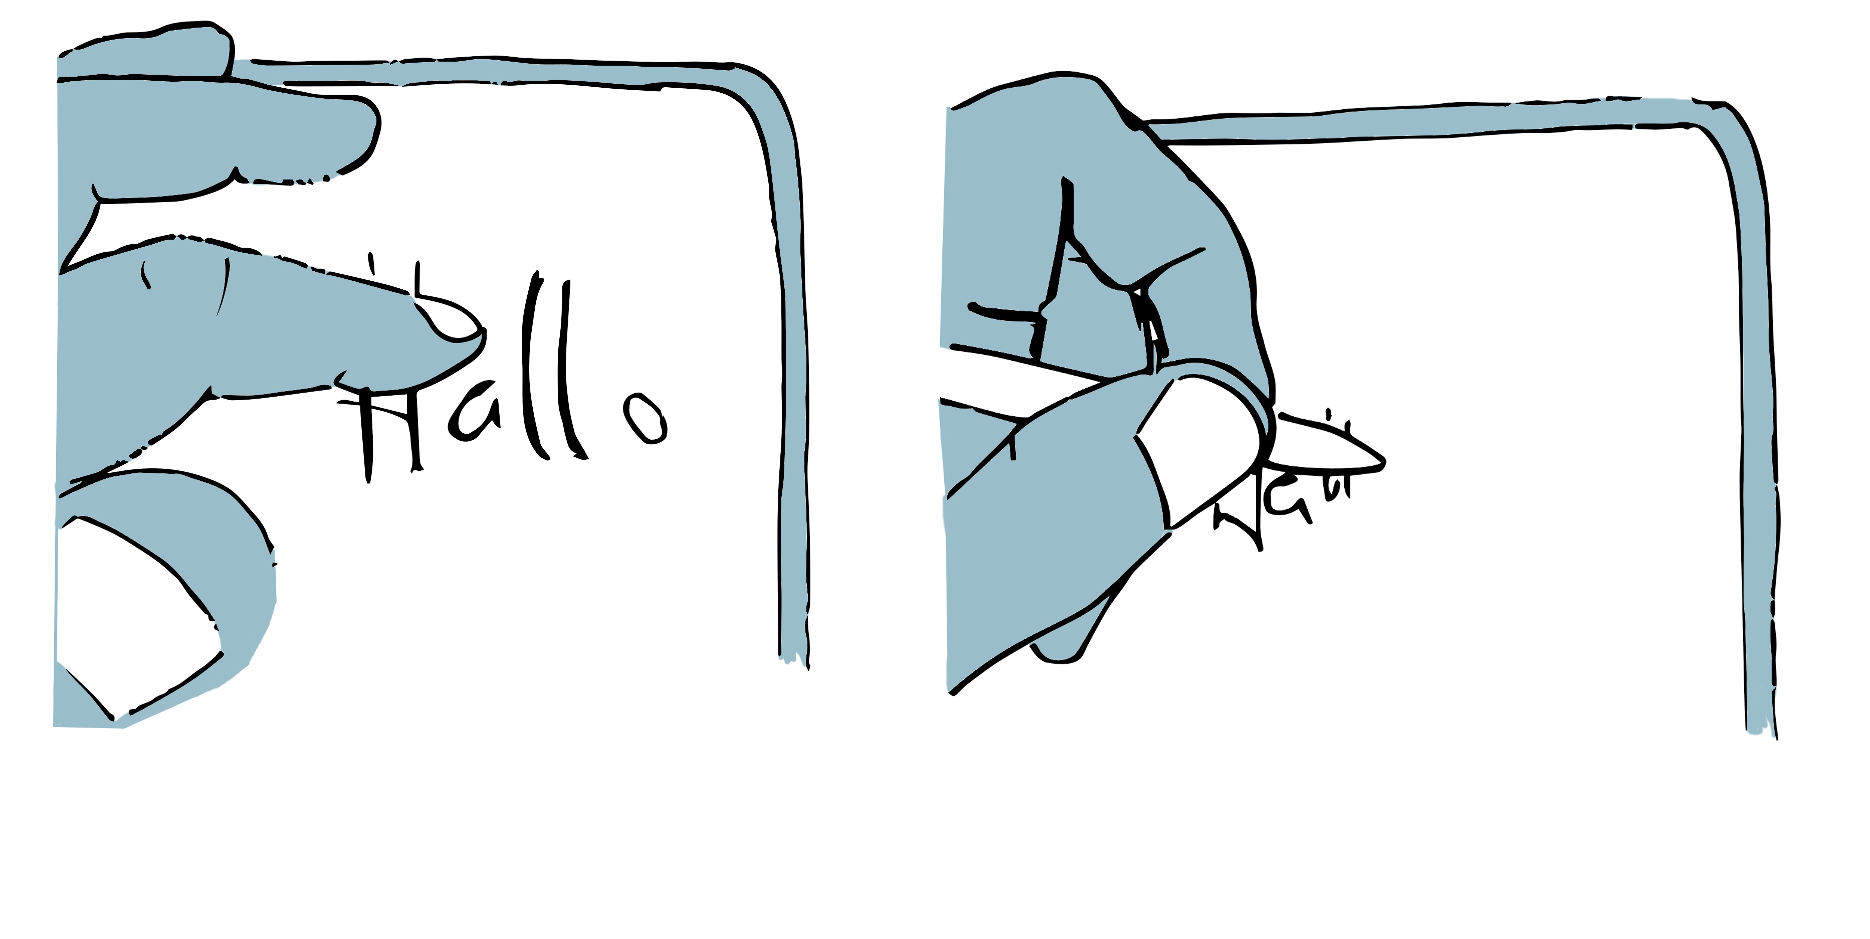
\includegraphics{Figures/11-03-Diskussionspunkt} \end{center}

\begin{blackbox}
\emph{Was ist eigentlich die ›natürlichste‹ Art, in einem digitalen Medium zu schreiben?}

\end{blackbox}

\section{Kartierung von Benutzungsflüssen}\label{kartierung-von-benutzungsfluxfcssen}

\textbf{Ziel}

Benutzungsflüsse dienen der Darstellung der Interaktionen, die Anwender*innen bei der Durchführung einer Handlung mit einem technischen Artefakt durchlaufen.

\textbf{Leitgedanke}

Die Kartierung von Benutzungsflüssen basiert auf der Idee, dass Anwender*innen bei der Nutzung digitaler Technologien für gewöhnlich eine Reihe von Schritten durchlaufen müssen, um die von ihnen intendierten Handlungen auszuführen. Bei jedem dieser Schritte müssen sie mit der Technologie über die jeweils vorhandenen Benutzungsschnittstellen interagieren. Die für die einzelnen Schritte notwendigen Interaktionen basieren auf den Gestaltungsentscheidungen der Entwickler*innen wie auch auf (kulturellen) Konventionen und Erwartungen der Anwender*innen.

\textbf{Anwendungskontext}

Benutzungsflüsse eignen sich sowohl zur Beschreibung aktueller wie auch antizipierter Interaktionsprozesse.

\begin{center}\includegraphics{Figures/11-04-Benutzungsflüsse} \end{center}

\textbf{Arbeitsschritte}

\begin{enumerate}
\def\labelenumi{\arabic{enumi}.}
\tightlist
\item
  Auswahl des zu kartierenden Prozesses.
\item
  Identifikation zentraler Handlungsschritte und hiermit einhergehender Interaktionen.
\item
  Dokumentation der einzelnen Prozessschritte mit Hilfe von Fotos, Screenshots oder Entwurfszeichnungen der jeweiligen Benutzungsschnittstellen.
\item
  Kurzbeschreibung der einzelnen Prozessschritte und Visualisierung des Verlaufs.
\end{enumerate}

\textbf{Ergebnisformat}

Ein Diagramm des Benutzungsflusses anhand von Fotos, Screenshots oder Entwurfszeichnungen der jeweiligen Benutzungsschnittstellen.

\textbf{Praktische Tipps}

\begin{itemize}
\tightlist
\item
  Benutzungsflüsse sollen die zur Durchführung einer Handlungen notwendigen Interaktionen möglichst detailliert darstellen.
\item
  Es soll deutlich werden, welche Fähigkeiten und Kenntnisse für die jeweilige Interaktion erforderlich sind.
\end{itemize}

\textbf{»Fallstricke«}

\begin{itemize}
\tightlist
\item
  Bei der Dokumentation der Interaktionen ist zu überlegen, wie sich diese am besten darstellen lassen. Screenshots reichen hier unter Umständen nicht aus.
\end{itemize}

\textbf{Weiterführende Literatur zum Leittext}

Vang, D. (2018, 22. April. User Journey v. User Flow - Dan Vang. Medium.
\url{https://medium.com/@danvang/user-journey-vs-user-flow-d5f32ae6c555}

\chapter{Soziotechnische Milieus \& Subjektivierung}\label{soziotechnische-milieus-subjektivierung}

Wie bei allen technischen Dingen ist auch die Existenz und Funktion digitaler Technologien an spezifische und auf sie abgestimmte Rahmenbedingungen gekoppelt. Neben geeigneten Ressourcen, Infrastrukturen und Produktionsbedingungen bedarf es hierfür sowohl entsprechender Fertigkeiten und Kenntnisse der Anwender*innen wie auch sozial geteilter Deutungs- und Handlungsmuster, die den praktischen Einsatz der technischen Artefakte ermöglichen und zugleich regulieren.

\begin{figure}

{\centering 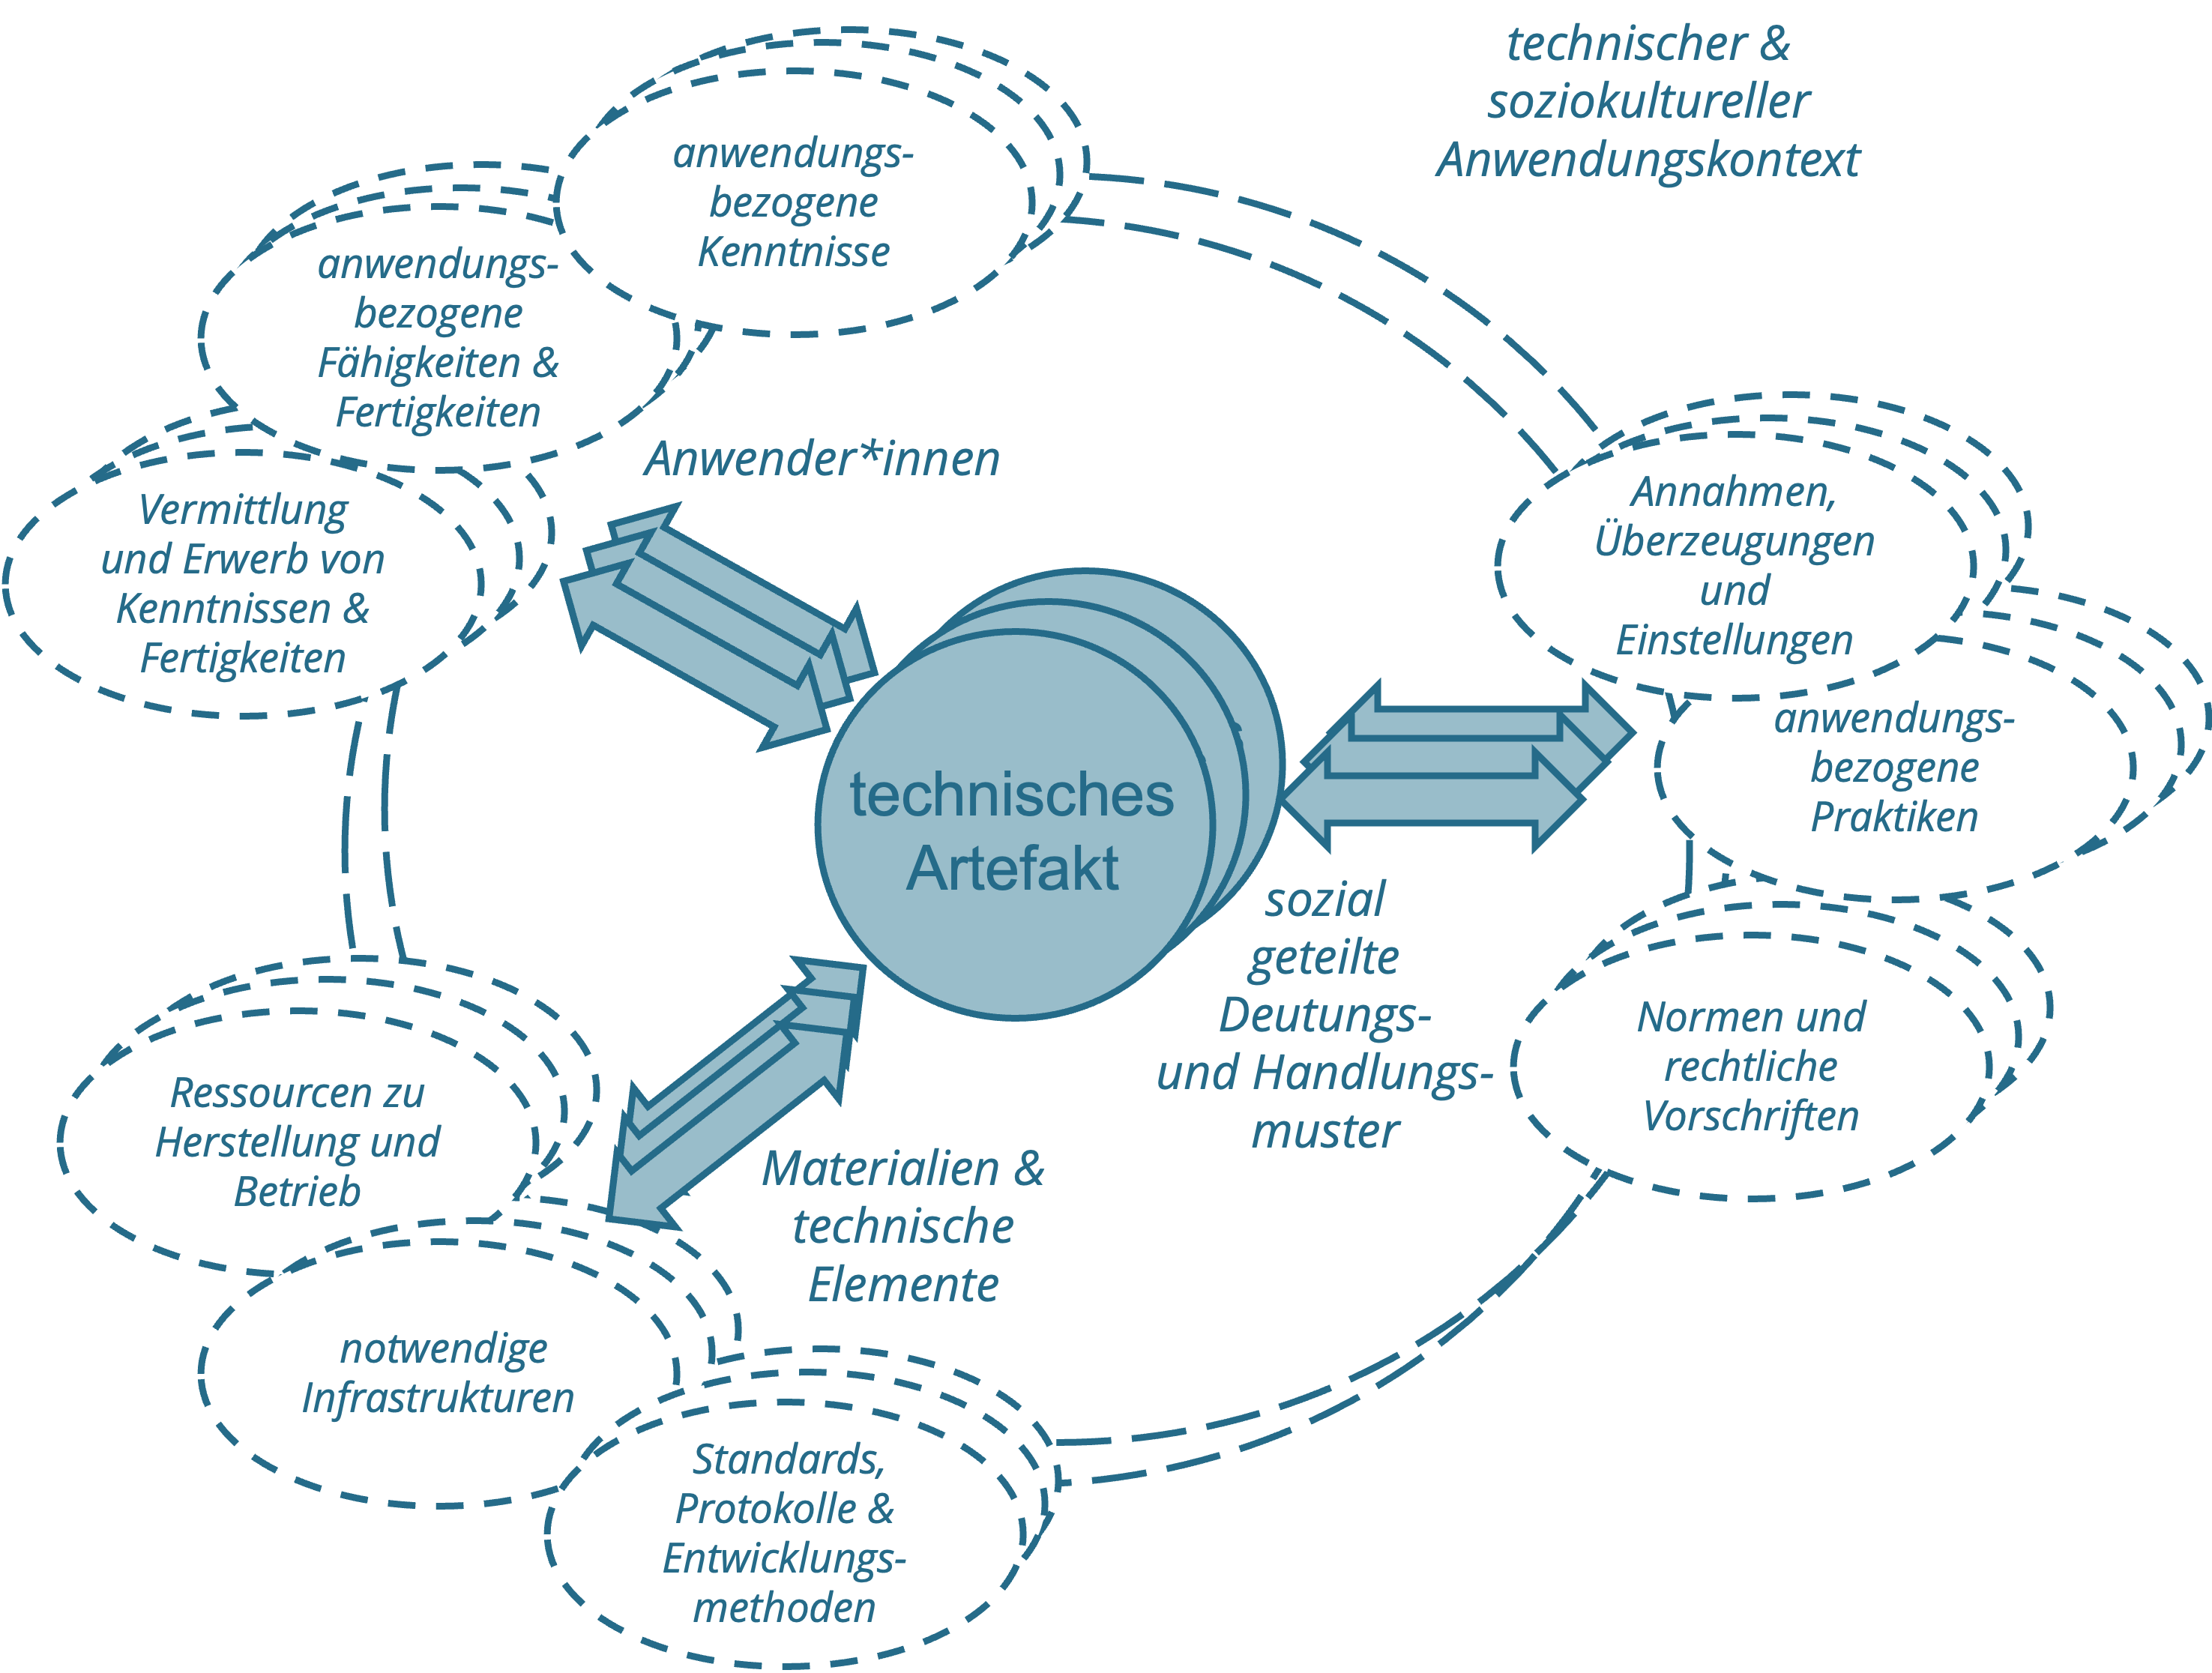
\includegraphics{Figures/12-01-SoziotechnischeMilieus} 

}

\caption{Strukturelemente soziotechnischer Milieus.}\label{fig:fig19}
\end{figure}

\section{Digitale Technologien und ihre assoziierten soziotechnischen Milieus}\label{digitale-technologien-und-ihre-assoziierten-soziotechnischen-milieus}

Obwohl es weitgehend unstrittig ist, dass technische und damit auch digitale Artefakte nicht aus sich selbst heraus existieren und funktionieren, so unterscheiden sich doch die Vorstellungen hinsichtlich der Beziehung zwischen den technischen Dingen und ihrer ›Umwelt‹.

Während klassische ingenieurswissenschaftliche Ansätze diese Beziehung vor allem im Sinne einer Anpassung der technischen Artefakte an gegebene Umweltbedingungen konzipieren, unterstellen insbesondere kulturwissenschaftlich orientierte Ansätze komplexe und reziproke Anpassungsprozesse zwischen den Dingen und ihrer Umwelt \citep[vgl. z.B.][]{akrichDescriptionTechnicalObject1992}. Kulturwissenschaftlich orientierte Ansätze gehen insofern davon aus, dass die Entwicklung und der Gebrauch technischer Artefakte nicht nur durch die jeweiligen Umweltbedingungen (mit-)bestimmt ist, sondern dass die Artefakte selbst Einfluss auf die Umwelten nehmen, in denen sie eingesetzt werden.

Der französische Technikphilosoph Gilbert Simondon hat diesen Gedanken zugespitzt, indem er davon ausgeht, dass die Entwicklung anwendungsfähiger technischer Artefakte immer auch mit der Ausbildung ›assoziierter Milieus‹ einhergeht. Aus der von Simondon entwickelten Perspektive erlangen die technischen Dinge ihre Funktion und Bedeutung erst mit der Ausbildung entsprechender Milieus, die zwar mit der Technikentwicklung einhergehen aber nicht gezielt hergestellt werden können \citep{simondonExistenzweiseTechnischerObjekte2012}.

Wie verschiedene Autor*innen im Anschluss an Simondon argumentieren, haben die mit einer Technologie assoziierten Milieus nicht nur eine technische und natürliche, sondern immer auch eine soziale und kulturelle Dimension \citep[vgl. z.B.][]{delitzGilbertSimondonsTheorie2012, hoelOntologicalForceTechnicity2013, huiWhatDigitalObject2012, mackenzieProblematisingTechnologicalObject2005}. Eine ähnliche Überlegung findet sich in Christiane Floyds Konzept der »Informatisierung des Gegenstandsbereichs« \citep[S. 245]{floydAutooperationaleFormUnd1997} im Zuge der Entwicklung digitaler Technologien wieder.

Der \textbf{Begriff des Milieus} ist sowohl in den Natur- wie auch den Sozial- und Kulturwissenschaften weit verbreitet und wird häufig synonym mit Begriffen wie Umwelt oder Kontext verwendet. Während die Begriffe Umwelt und Kontext oftmals als eine Art Hintergrund oder Rahmen verstanden werden, vor oder in dem ein bestimmtes Objekt oder ein Organismus existiert, unterläuft der Begriff des Milieus die Unterscheidung zwischen Organismus und Umwelt, bzw. Objekt und Kontext. Der Begriff des Milieus, im hier verwendeten Sinn, betont vielmehr den Umstand, dass das Milieu, von dem ein Organismus oder auch ein technisches Objekt abhängig ist, durch den Organismus bzw. das Objekt selbst organisiert und hervorgebracht wird. Das Milieu ist insofern »a pure system of relations without supports« \citep[S. 103]{canguilhemKnowledgeLife2008}.

Die assoziierten Milieus technischer Artefakte umfassen unter anderem (a) entwicklungstechnische Konventionen und Vereinbarungen, wie \textbf{Standards, Protokolle und Methoden}, (b) \textbf{Ressourcen} zu Herstellung und Betrieb der technischen Dinge, (c) \textbf{Infrastrukturen} in bzw. auf denen sie operieren können, (d) sozial geteilte und sanktionierte \textbf{Normen und (rechtliche) Vorschriften} zum Gebrauch der Artefakte, (e) sozial geteilte \textbf{Überzeugungen und Einstellungen} zur Bedeutung und Funktion der Dinge, (f) kollektive und auf die Technologie abgestimmte \textbf{Praktiken}, (g) anwendungsbezogene \textbf{Fertigkeiten und Fähigkeiten}, (h) anwendungsbezogene \textbf{Kenntnisse} sowie (i) \textbf{Verfahren zur Vermittlung und zum Erwerb} der im Umgang mit den Artefakten notwendigen Kenntnisse und Fertigkeiten (siehe {Abb. 12.1}).

\section{Digitale (Medien-)Ideologien und Modelle des Menschen}\label{digitale-medien-ideologien-und-modelle-des-menschen}

Wie bereits angedeutet haben die assoziierten Milieus technischer Artefakte nicht nur eine technische und natürliche, sondern immer auch eine soziale und kulturelle Dimension. Es bedarf nicht zuletzt entsprechender sozial geteilter Überzeugungen, Einstellungen und Praktiken, damit eine Technologie ihre jeweilige Bedeutung und Funktion erlangen kann.

Die Anthropologin Ilana Gershon hat für die auf Technologien beziehungsweise Medien bezogenen Überzeugungen und Einstellungen den Begriff der ›Medienideologien‹ geprägt \citep[vgl.][]{gershonMediaIdeologiesIntroduction2010}. \textbf{Medienideologien} sind für Gershon das Produkt unserer praktischen und kollektiv geteilten Erfahrungen und prägen unseren Umgang mit digitalen Technologien.

Während Gershon die Bedeutung lokaler Praktiken für die Ausbildung von Medienideologien betont, haben andere Autor*innen darauf hingewiesen, dass sich in der Verbreitung digitaler Technologien auch grundlegendere \textbf{kulturelle Deutungsmuster} widerspiegeln. So hat etwa Christiane Floyd darauf argumentiert, dass in der Ausbildung (auto-)operationaler Formen typisch ›westliche‹ Deutungs- und Handlungsmuster zum Ausdruck kommen, in denen die Regelhaftigkeit und Formalisierbarkeit von Prozessen betont wird \citep[vgl.][]{floydDevelopingEmbeddingAutoOperational2002}. In ähnlicher Weise hat etwa Bettina Heintz darauf hingewiesen, dass auch der »Erfolg der Künstlichen Intelligenz {[}\ldots{]} nicht so sehr eine technische als vielmehr eine soziale Angelegenheit {[}ist{]}« \citep[vgl.][S. 289]{heintzHerrschaftRegelZur1993}, die letztlich davon abhängt, wie wir uns selbst zu diesen Technologien in Beziehung setzen und wie wir uns selbst und unsere Rolle in der Welt verstehen.

Technische Artefakte und die mit ihnen assoziierten Milieus beinhalten dementsprechend auch immer spezifische \textbf{Modelle des Menschen}. Diese Modelle umfassen etwa Annahmen darüber, wer wir als Menschen sind, was wir können und in welchem Verhältnis wir zu uns, zu anderen wie auch zur (technischen) Welt stehen. Hiermit einher gehen Fragen nach der Identität, Autonomie und Handlungsträgerschaft des Menschen, seiner ›(Un-)Berechenbarkeit‹, wie auch der (Chancen-)Gleichheit und der Verteilung von Macht \citep[ausführlicher hierzu auch][]{sesinkMenschlicheUndKunstliche2012}.

Auch wenn in der aktuellen wissenschaftlichen Diskussion unterschiedliche Positionen hinsichtlich der Frage vertreten werden, inwiefern entsprechende Medienideologien und Modelle des Menschen durch die Entwickler*innen in die technischen Artefakte ›eingeschrieben‹ werden oder ob sie sich erst im praktischen Gebrauch manifestieren, so ist doch weitgehend unstrittig, dass die technischen Dinge und damit auch die digitalen Technologien keine neutralen Werkzeuge und Instrumente sind, derer wir uns nach Belieben bedienen können. Die technischen Dinge sind vielmehr immer schon Bestandteil und Ausdruck kultureller Entwicklungslinien.

Fragen nach den ›technischen Weltverhältnissen‹ \citep{zornSelbstWeltUnd2014} kommt dementsprechend in der (medien-)pädagogischer Diskussion eine sehr zentrale Rolle zu.

\begin{blackbox}
\emph{Welche pädagogischen Implikationen ergeben sich aus der Verwicklung des Menschen in die technischen Weltverhältnisse im Kontext Schule?}

\end{blackbox}

~

\begin{center}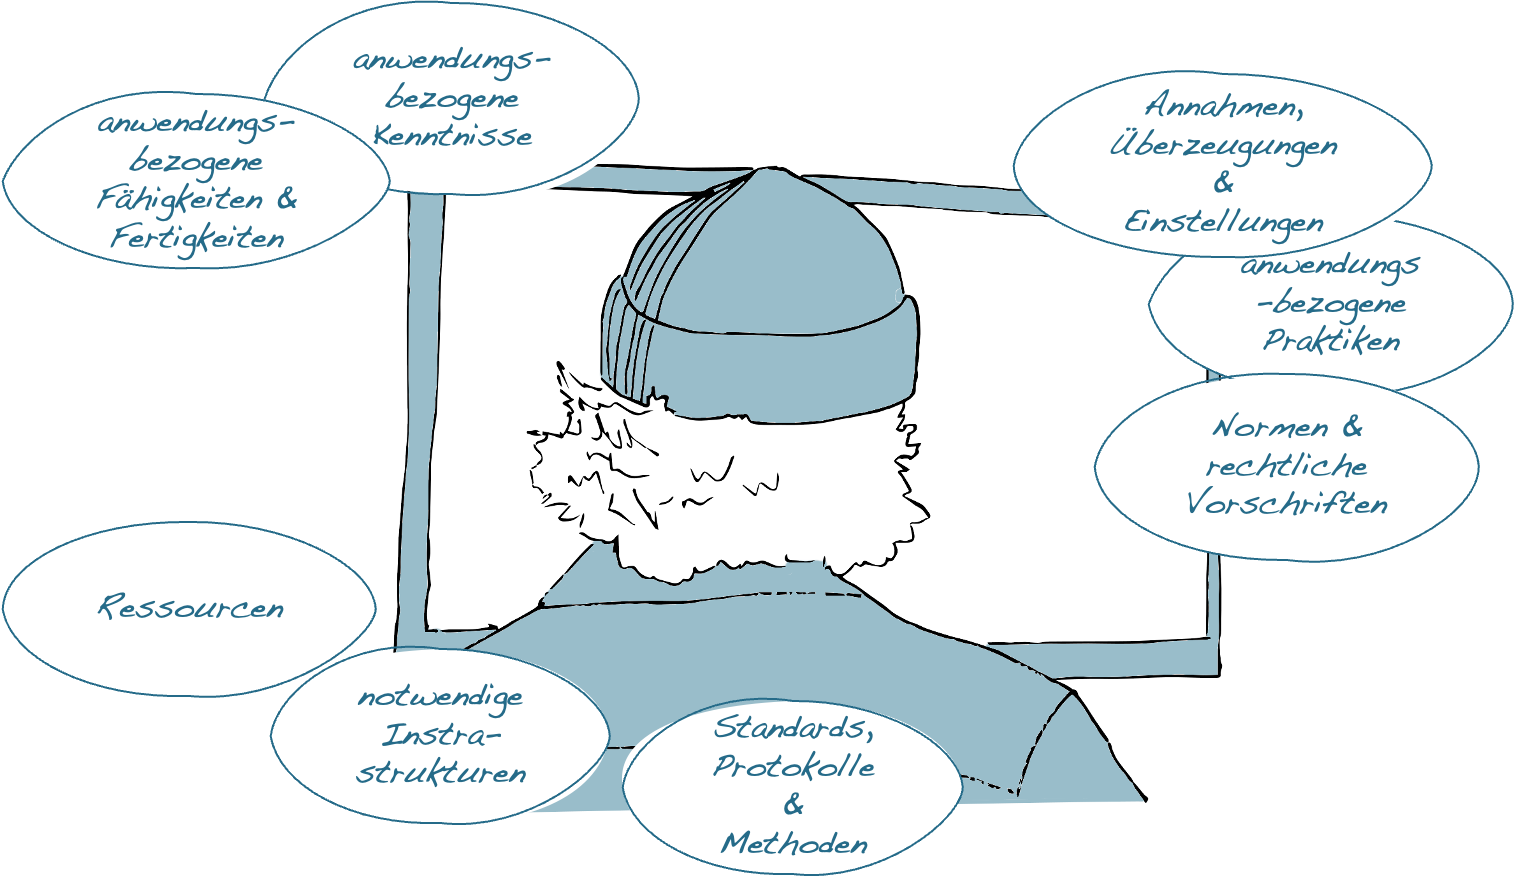
\includegraphics{Figures/12-02} \end{center}

\begin{blackbox}
\emph{Wie ist eigentlich das assoziierte Milieu einer Power-Point-Präsentation im Unterricht beschaffen?}

\end{blackbox}

\section{Kartierung assoziierter Milieus technischer Artefakte}\label{kartierung-assoziierter-milieus-technischer-artefakte}

\textbf{Ziel}

Die Kartierung assoziierter Milieus dient der Verortung technischer Artefakte und der Darstellung grundlegender Rahmenbedingungen.

\textbf{Leitgedanke}

Die Kartierung assoziierter Milieus dient dazu, die für die praktische Einsatzfähigkeit eines technischen Artefakts grundlegenden Rahmenbedingungen zu identifizieren. Die assoziierten Milieus sind dabei zugleich Voraussetzung wie auch Produkt des jeweiligen Artefakts. Neben der Benennung und ›Verortung‹ des technischen Artefakts, gehen hierbei auch die anwendungsbezogene Fertigkeiten und Kenntnisse der Nutzer*innen, materielle Voraussetzungen sowie kollektive Deutungs- und Handlungsmuster in die Kartierung mit ein.

\textbf{Anwendungskontext}

Die Kartierung assoziierter Milieus eignet sich zum Abstecken eines Gegenstandsbereichs und bietet einen Ausgangspunkt für weiterführende Analysen.

\begin{center}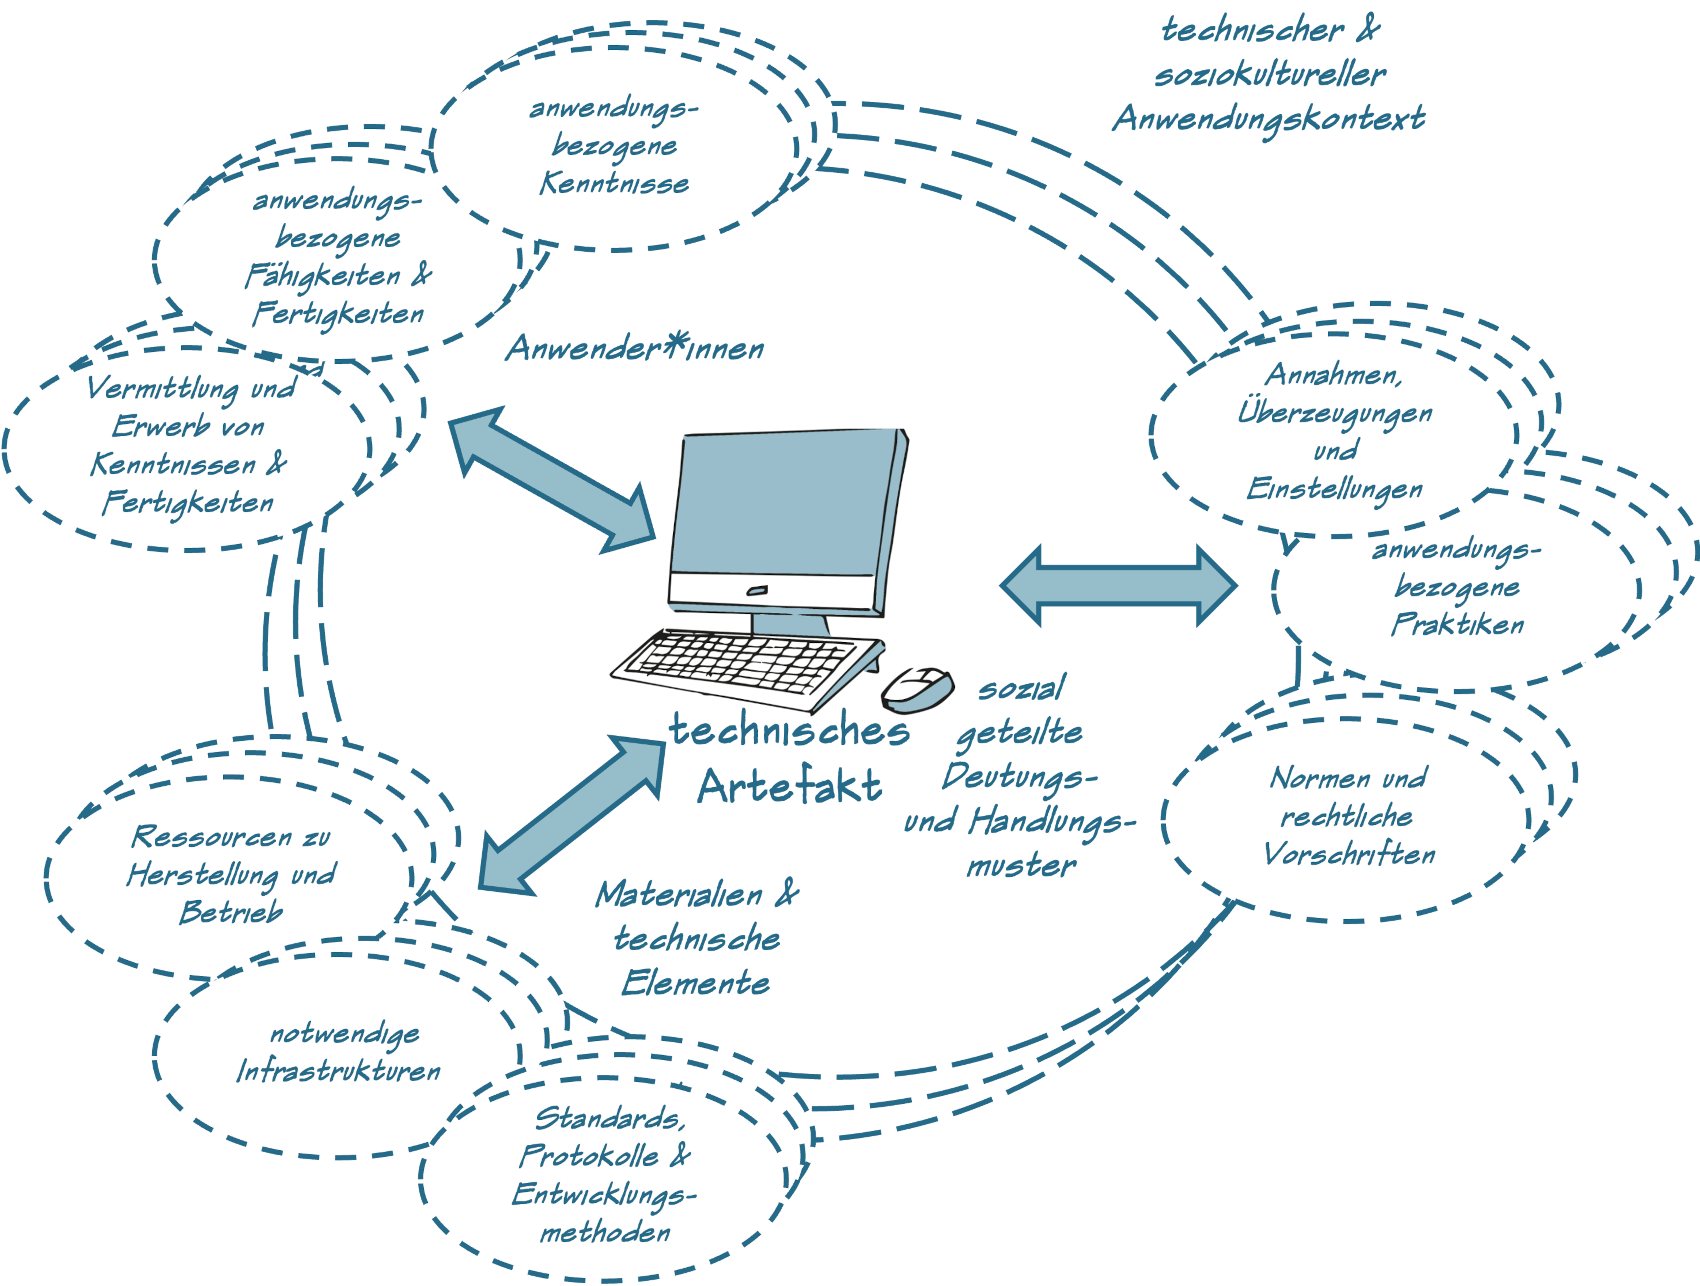
\includegraphics{Figures/12-03-Leittext Milieu} \end{center}

\textbf{Arbeitsschritte}

\begin{enumerate}
\def\labelenumi{\arabic{enumi}.}
\tightlist
\item
  Auswahl des technischen Artefakts, dessen Milieu kartiert werden soll.
\item
  ›Verortung‹ des Artefakts: In welchem technischen und kulturellen Anwendungskontext wird das Artefakt analysiert?
\item
  Beschreibung und ggf. Illustration wesentlicher Strukturelemente, die für die praktische Einsatzfähigkeit des Artefakts existenziell sind.
\item
  Ggf. Überarbeitung oder Erweiterung der Karte.
\end{enumerate}

\textbf{Ergebnisformat}

Eine grafische, evtl. mit Bildern oder Verweisen angereicherte Darstellung der wesentlichen Strukturelemente.

\textbf{Praktische Tipps}

\begin{itemize}
\tightlist
\item
  Die Karte sollte Außenstehenden eine Idee von den für den praktischen Gebrauch der jeweiligen Technologie notwendigen Voraussetzungen vermitteln.
\item
  Die Beschreibung sollte sich an den Begrifflichkeiten der beteiligten Akteur*innen orientieren.
\end{itemize}

\textbf{»Fallstricke«}

\begin{itemize}
\tightlist
\item
  Die technischen Artefakte und ihre Milieus sind keine fixen Entitäten, sondern unterliegen permanenten Veränderungen. Eine entsprechende Kartierung stellt deshalb bestenfalls eine lokale Momentaufnahme dar.
\item
  Die Strukturelemente der assoziierten Milieus technischer Artefakte ähneln denen sozialer Praktiken. Dies ist darin begründet, dass soziale Praktiken zum Milieu technischer Artefakte gehören und umgekehrt.
\end{itemize}

\textbf{Weiterführende Literatur zum Leittext}

Hui, Y. (2012). What is a digital object? Metaphilosophy, 43(4), 380--395.

Shove, E.,Pantzar, M., \& Watson, M. (2012). The Dynamics of Social Practice --- Everyday Life and how it Changes. Los Angeles: Sage.

\chapter{Schulische Medienbildung \& Kompetenzen}\label{schulische-medienbildung-kompetenzen}

Mit der zunehmenden Digitalisierung privater, öffentlicher und beruflicher Lebenswelten wie auch der Möglichkeiten zum Einsatz digitaler Technologien im Unterricht, stellt sich die Frage nach dem Beitrag, den die Institution Schule zu einer zeitgemäßen digitalen Medienbildung leisten kann und soll. Hierbei geht es sowohl um den Einsatz digitaler Technologien als Werkzeuge und Medien im Unterricht wie auch die Auseinandersetzung mit Prozessen der Digitalisierung als Unterrichtsgegenstand.

Im Folgenden werden anhand der »Ergänzungen zu den Fachanforderungen Medienkompetenz --- Lernen mit digitalen Medien« \citep{ministeriumfurbildungwissenschaftundkulturdeslandesschleswig-holsteinErganzungenFachanforderungenMedienkompetenz2018} die Verankerung der ›digitalen Medienbildung‹ als Teil des schulischen Bildungsauftrags sowie die Grundstruktur des hiermit einhergehen Kompetenzrasters dargestellt. Dem hiermit verbundenen funktional-pragmatischen Kompetenzbegriff wird anschließend ein sozial-kollektives Verständnis von Kompetenzen gegenübergestellt.

\begin{center}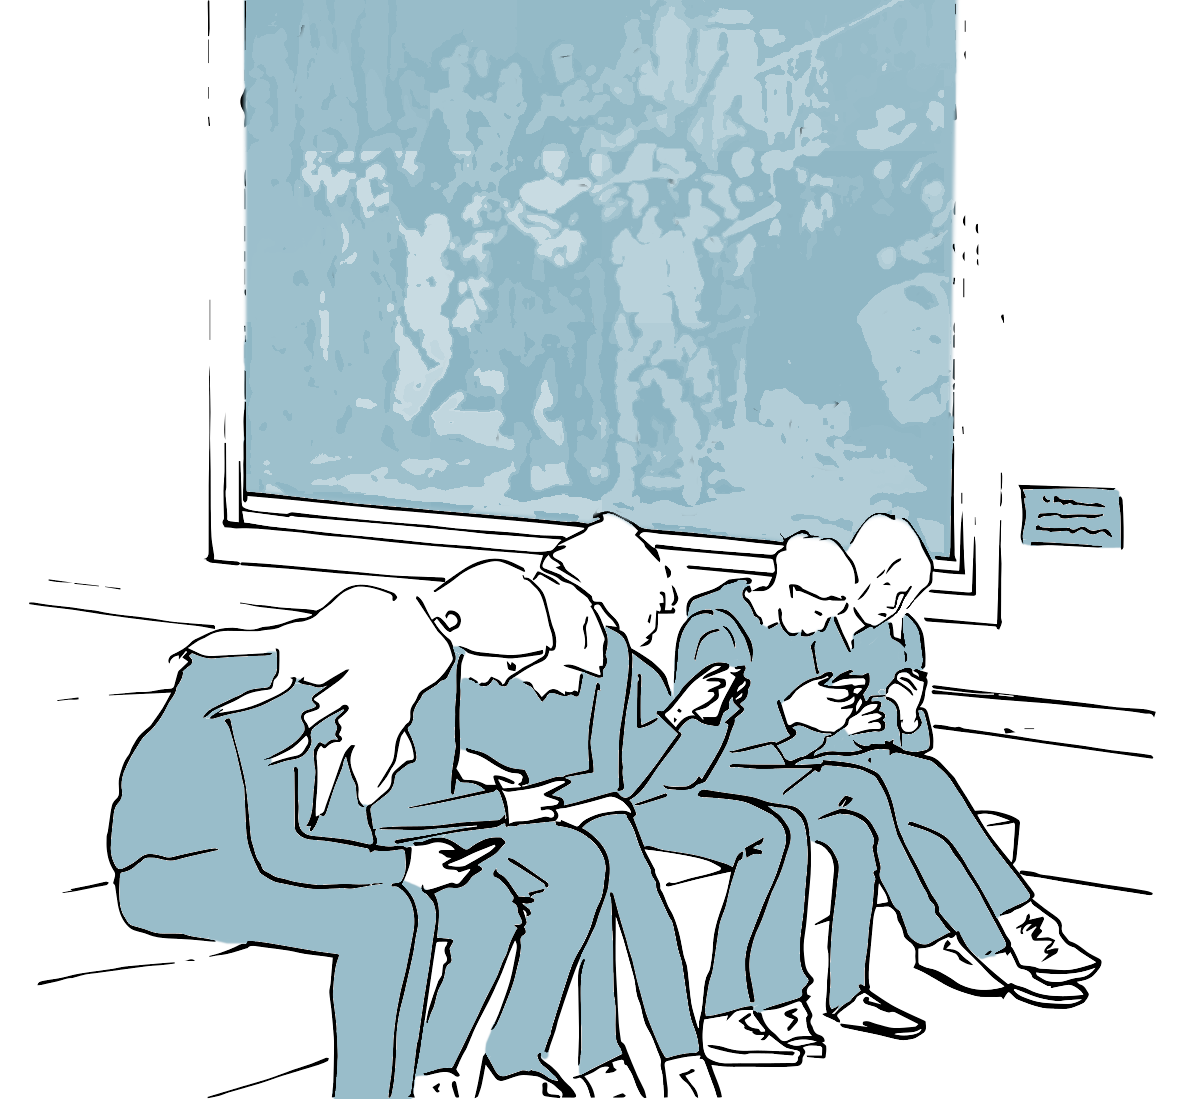
\includegraphics{Figures/13-01-Kompetenz-Color} \end{center}

\section{Digitale Medienbildung als Teil des schulischen Bildungsauftrags}\label{digitale-medienbildung-als-teil-des-schulischen-bildungsauftrags}

Die curriculare Einbindung der digitalen Medienbildung in den Schulunterricht ist in Schleswig-Holstein durch die »Ergänzungen zu den Fachanforderungen Medienkompetenz --- Lernen mit digitalen Medien« \citep{ministeriumfurbildungwissenschaftundkulturdeslandesschleswig-holsteinErganzungenFachanforderungenMedienkompetenz2018} geregelt. Die Fachanforderungen orientieren sich dabei an dem von der Kultusministerkonferenz 2016 verabschiedeten Strategiepapier »Bildung in der digitalen Welt« \citep{kultusministerkonferenzBildungDigitalenWelt2016} und konkretisieren dieses.

Ausgangspunkt dieser Dokumente bildet hierbei die \textbf{Diagnose einer umfassenden ›Digitalisierung aller Lebensbereiche‹}, der auch die Schule Rechnung tragen muss, wenn sie ihrem Bildungs- und Erziehungsauftrag gerecht werden will, der darin besteht:

{»Schülerinnen und Schüler angemessen auf das Leben in der derzeitigen und künftigen Gesellschaft vorzubereiten und sie zu einer aktiven und verantwortungsvollen Teilhabe am kulturellen, gesellschaftlichen, politischen, beruflichen und wirtschaftlichen Leben zu befähigen.« \citep[S. 10]{kultusministerkonferenzBildungDigitalenWelt2016}}

Digitale Technologien bzw. Medien sind aus schulischer Perspektive dabei sowohl in Bezug auf ihren Einsatz zur \textbf{Unterstützung von Lernprozessen} (digitale Technologien als Werkzeuge und Mittel des Unterrichts) und wie auch als \textbf{Thema von Unterricht} (digitale Technologien als Unterrichtsgegenstand) von Bedeutung. In den Fachanforderungen des Landes Schleswig-Holstein wird der diesbezügliche \textbf{Zielhorizont} wie folgt definiert:

{»Schülerinnen und Schüler lernen selbstbestimmt, sachgerecht, sozial verantwortlich, kommunikativ, produktiv und kreativ gestaltend mit digitalen Medien umzugehen. Sie reflektieren ihren eigenen Umgang mit den Medien und setzen sich kritisch mit Inhalten der digitalen Welt auseinander. Hierbei ist verantwortliche, auf demokratischem Grundverständnis basierende Mitgestaltung und Auseinandersetzung mit den kontinuierlich entstehenden Inhalten und Strukturen wesentlich.« \citep[S. 4]{ministeriumfurbildungwissenschaftundkulturdeslandesschleswig-holsteinErganzungenFachanforderungenMedienkompetenz2018}}

Der hierfür notwendige Erwerb von Kenntnissen und Fähigkeiten sowie damit verbundener Kompetenzen wird hierbei als eine fächerübergreifende Aufgabe verstanden, die keinem »isolierten Lernbereich oder Unterrichtsfach zugeordnet werden {[}kann{]}« \citep[S. 10]{ministeriumfurbildungwissenschaftundkulturdeslandesschleswig-holsteinErganzungenFachanforderungenMedienkompetenz2018}, sondern »integraler Bestandteil eines jeden Fachs ist« \citep[S. 4]{ministeriumfurbildungwissenschaftundkulturdeslandesschleswig-holsteinErganzungenFachanforderungenMedienkompetenz2018}. Die Auseinandersetzung mit Fragen der Digitalisierung ist insofern in die einzelnen Unterrichtsfächer zu integrieren.

Aufbauend auf diesen Überlegungen hat die Kultusministerkonferenz mit ihrem Strategiepapier »Bildung in der digitalen Welt« einen \textbf{Kompetenzrahmen} erstellt, der auf den oberen Abstraktionsebenen die folgenden sechs Kompetenzbereiche umfasst:

{\textbf{K1: Suchen, Verarbeiten, Aufbewahren}}

{\textbf{K2: Kommunizieren und Kooperieren}}

{\textbf{K3: Produzieren und Präsentieren}}

{\textbf{K4: Schützen und sicher Agieren}}

{\textbf{K5: Problemlösen und Handeln}}

{\textbf{K6: Analysieren und Reflektieren}}

Für die weitere Ausdifferenzierung und die Abbildung auf die unterschiedlichen Schulstufen siehe die Fachanforderungen für Schleswig Holstein \citep{ministeriumfurbildungwissenschaftundkulturdeslandesschleswig-holsteinErganzungenFachanforderungenMedienkompetenz2018}.

\section{Funktional-pragmatische und sozial-kollektive Modelle der Medienkompetenz}\label{funktional-pragmatische-und-sozial-kollektive-modelle-der-medienkompetenz}

Modelle der Medienkompetenz, wie sie auch den ›Fachanforderungen Medienkompetenz‹ \citep{ministeriumfurbildungwissenschaftundkulturdeslandesschleswig-holsteinErganzungenFachanforderungenMedienkompetenz2018} zu Grunde liegen, orientieren sich an einem individuumsbezogenen, funktional-pragmatischen Kompetenzbegriff. Sie gehen davon aus, dass (Medien-)Kompetenzen im Wesentlichen auf explizit lehr- und lernbaren Wissensbeständen beruhen, die weitgehend kontextunabhängig gültig sind, allgemeinen Gütekriterien genügen und sich als Besitz oder Eigenschaft einer Person verstehen lassen \citep{alkemeyerBefahigenPraxistheoretischeUberlegungen2017, blohRekonstruktiveEvaluationsforschungIm2022}.

Ungeachtet seiner weiten Verbreitung im bildungspolitischen und erziehungswissenschaftlichen Diskurs, bringt ein derartiger Kompetenzbegriff jedoch eine Reihe theoretischer wie auch pädagogischer Herausforderungen mit sich. So stellt sich beispielsweise die Frage, inwieweit ein kontextunabhängiges Verständnis von Medienkompetenz und die Festlegung standardisierter Bewertungskriterien sowohl der Heterogenität medialer Praktiken als auch deren schnellem Wandel Rechnung tragen kann und wer darüber bestimmt, welche Kompetenzen es letztlich auszubilden gilt \citep{kammerlEnkulturationshilfenDigitalenGesellschaft2014}. Ebenso besteht die Gefahr, dass Fragen der Medienkompetenz individualistisch verkürzt und die überindividuelle, gesellschaftliche und kulturelle Dimension medialer und digitaler Transformationsprozesse aus dem Blick gerät \citep{baackeMedienkompetenzBegrifflichkeitUnd1996}. Darüber hinaus wirft die funktional-pragmatische Verkürzung des Kompetenzbegriffs die Frage auf, wie neben der Befähigung zu Teilhabe an bestehenden Praktiken auch die Möglichkeit zur kritischen Reflexion, aktiven Mitgestaltung und nachhaltigen Transformation eben dieser Praktiken gefördert werden kann.

Vor diesem Hintergrund finden sich in der pädagogischen Diskussion vermehrt Positionen, die einen sozial-kollektiven Kompetenzbegriff vertreten und (Medien-)Kompetenzen als Produkt sozialer Praktiken zu verstehen, das sich im wiederholten und gemeinsamen miteinander ausbildet und infolgedessen kontextuell gebunden ist. Kompetenz ist aus dieser Perspektive immer schon sozial und kulturell vermittelt, beinhaltet immer auch inkorporiertes und implizites Wissen und bedarf der sozialen Anerkennung durch andere \citetext{\citealp{blohRekonstruktiveEvaluationsforschungIm2022}; \citealp[vgl.][]{huggerMedienkompetenz2022}}. Die Ausbildung entsprechender Kompetenzen ist hierbei nicht lediglich ein affirmativer Prozess der Anpassung an gegeben kulturelle Formen, sondern ein Prozess der aktiven Aneignung, in dem die Kompetenzen produktiv genutzt werden, um die jeweiligen Praktiken fortzusetzen und auch zu transformieren \citep{lochEnkulturationAlsAnthropologischer1968}.

Die Entwicklung von (Medien-)Kompetenz ist aus dieser Perspektive immer schon bezogenen auf die konkreten (Medien-)Praktiken, in denen jeweiligen Akteur*innen, seien es Schüler*innen oder Lehrkräfte agieren. An die Stelle eines statischen Verständnisses vordefinierter (Medien-)Kompetenzen rückt damit ein dynamischer Zugang, der unter anderem danach fragt, (a) welche Kenntnisse, Fertigkeiten und Haltungen im Rahmen der jeweiligen Praktiken von Bedeutung sind, (b) an welchen Normen und Werten sich ein ›praktisch angemessenes‹ Tun festmacht, aber auch (c) wie diese Normen und Werte zu beurteilen sind und (d) welche Möglichkeiten zur Weiterentwicklung und Transformation der Praktiken sich auftun.

\begin{blackbox}

\emph{Wie gestaltet sich der ›kompetente‹ Umgang mit ChatGPT beim Schreiben der nächsten Hausarbeit?}

\begin{center}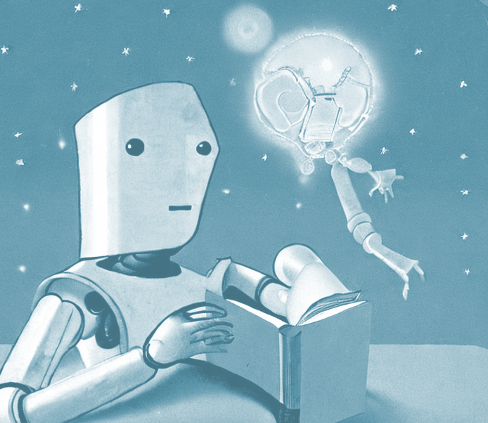
\includegraphics{Figures/13-02-ChatGPT} \end{center}

\begin{center}
*Stable Diffusion: »a robot reading its own mind, hieronymus bosch style."*
\end{center}

\end{blackbox}

~

\section{Erstellung praxisbezogener Kompetenzprofile}\label{erstellung-praxisbezogener-kompetenzprofile}

\textbf{Ziel}

Die Erarbeitung praxisbezogener Kompetenzprofile dient dazu, individuelle und kollektive Entwicklungshorizonte in Bezug auf eine bestimmte mediale Praxis zu identifizieren und zu bewerten.

\textbf{Leitgedanke}

Die Erstellung praxisbezogener Kompetenzprofile basiert auf einem sozial-kollektiven Kompetenzbegriff, der davon ausgeht, dass Kompetenzen ein Produkt sozialer Praktiken sind und infolgedessen nur in Bezug auf die jeweiligen Praktiken definiert werden können. Als Produkt sozialer Praktiken unterliegen Kompetenzen zudem einem permanenten Veränderungsdruck, da letztlich immer wieder neu von den Praktiker*innen in gegenseitiger Abstimmung entschieden werden muss, was als ›angemessen‹ bzw. ›kompetent‹ erachtet wird, beziehungsweise erachtet werden soll. Die Grundstruktur der Kompetenzprofile orientiert sich dabei grob an der von Dieter Baacke vorgeschlagenen Ausdifferenzierung der Medienkompetenz in Medien-Kritik, Medien-Kunde, Medien-Nutzung und Medien-Gestaltung, wobei diese Dimensionen hier jedoch praxistheoretisch interpretiert werden.

\textbf{Anwendungskontext}

Die Erstellung praxisbezogener Kompetenzprofile eignet sich sowohl als Vorarbeit zur Festlegung pädagogischer Ziele wie zur kollaborativen Reflexion und Evaluation unter Praktiker*innen.

\begin{center}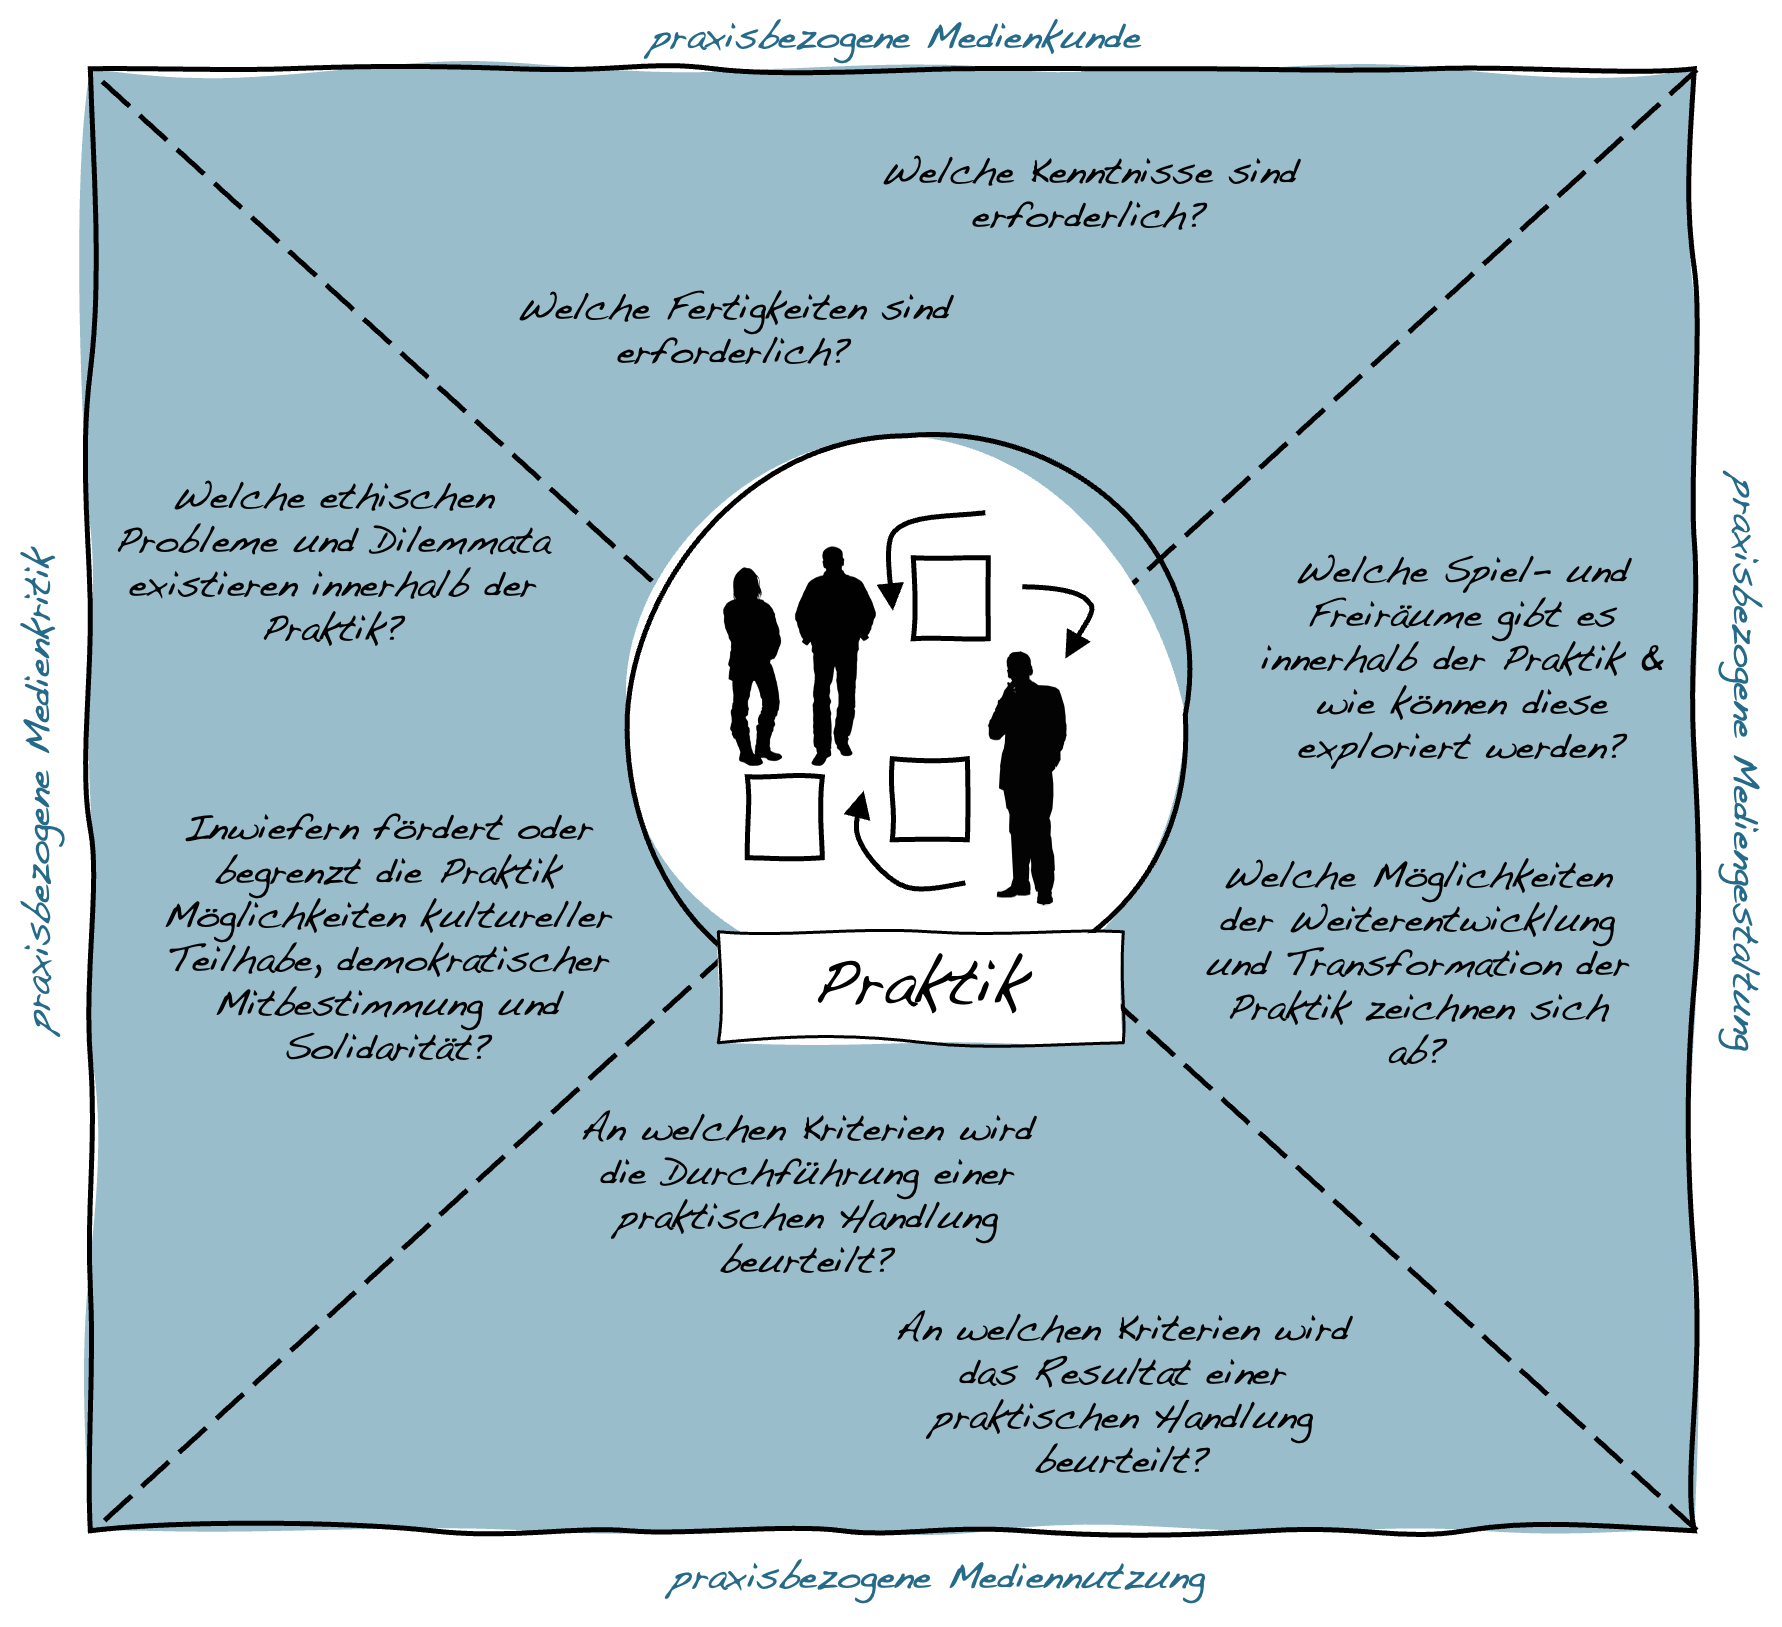
\includegraphics{Figures/13-03} \end{center}

\textbf{Arbeitsschritte}

\begin{enumerate}
\def\labelenumi{\arabic{enumi}.}
\tightlist
\item
  Auswahl und Konkretisierung der Praktik, für die ein Kompetenzprofil erstellt werden soll.
\item
  Sammlung von Informationen über die jeweilige Praktik, einschließlich von Beispielen guter und schlechter Praxis.
\item
  Vergleich mit angrenzenden und/oder ähnlichen Praktiken.
\item
  Austausch mit den Praktiker*innen über das erstellte Kompetenzprofil und eventuelle Überarbeitung.
\end{enumerate}

\textbf{Ergebnisformat}

Eine Übersicht des Kompetenzprofils.

\textbf{Praktische Tipps}

\begin{itemize}
\tightlist
\item
  Die Erstellung der praxisbezogenen Kompetenzprofile sollte in enger Abstimmung mit den Praktiker*innen erfolgen und auf ihre Beschreibungen und Begriffe Bezug nehmen.
\item
  Die einer sozialen Praktik zugrunde liegenden Normen und Werte sind oft impliziter Art. Eine vergleichende Betrachtung verschiedener Praktiken kann hilfreich sein, um Differenzen sichtbar werden zu lassen.
\end{itemize}

\textbf{»Fallstricke«}

\begin{itemize}
\tightlist
\item
  Die Anforderungen an praxisbezogene Kompetenzen unterliegen einem kontinuierlichem Wandel und können aufgrund ihres in Teilen impliziten Charakters nur ansatzweise beschrieben werden. Die Profile sollen entsprechend nicht den aktuellen Zustand festschreiben, sondern zu einer reflexiven Auseinandersetzung einladen und anregen.
\end{itemize}

\textbf{Weiterführende Literatur zum Leittext}

Baacke, D. (1996). Medienkompetenz -- Begrifflichkeit und sozialer Wandel. In A. von Rein (Hrsg.), \emph{Medienkompetenz als Schlüsselbegriff} (S. 112--124). Klinkhardt.

Bloh, T. (2022). Rekonstruktive Evaluationsforschung im Kontext praxeologischer Kompetenzdiskurse. Kritische Reflexionen und konzeptionelle Überlegungen zur Dokumentarischen Evaluationsforschung. \emph{Zeitschrift für Evaluation}, 21(2), 193--215.

\chapter{Schulische Medienbildung \& digitale Transformation}\label{schulische-medienbildung-digitale-transformation}

Die Vorstellung von der Digitalisierung als einem kulturellen Transformationsprozess, in dem digitale Technologien einen tiefgreifenden Einfluss auf unsere Erfahrungs- und Handlungsmöglichkeiten haben, wirft nicht nur die Frage auf, welche Kompetenzen in der Schule vermittelt werden sollen, sondern auch, wie mit digitalen Technologien in der Schule umgegangen werden soll und in welcher Form sie zum Gegenstand von Unterricht werden können.

Ohne an dieser Stelle eine abschließende Antwort auf diese Fragen geben zu können, sollen stattdessen einige Einsatzpunkte und Gedanken skizziert werden, die einerseits versuchen sich der Digitalisierung im Sinne eines ›epochaltypischen Schlüsselproblems‹ \citep{klafkiNeueStudienZur2007} als Gegenstand von Unterricht zu nähern und die andererseits den Umgang mit digitalen Technologien in der Schule in Hinblick auf Fragen von Macht, Mitbestimmung und Teilhabe thematisieren. Als Stichwortgeber dient in beiden Fällen eine Auswahl der vom Land Schleswig-Holstein beschriebenen Kompetenzen für Schüler*innen \citep{ministeriumfurbildungwissenschaftundkulturdeslandesschleswig-holsteinErganzungenFachanforderungenMedienkompetenz2018}.

\begin{center}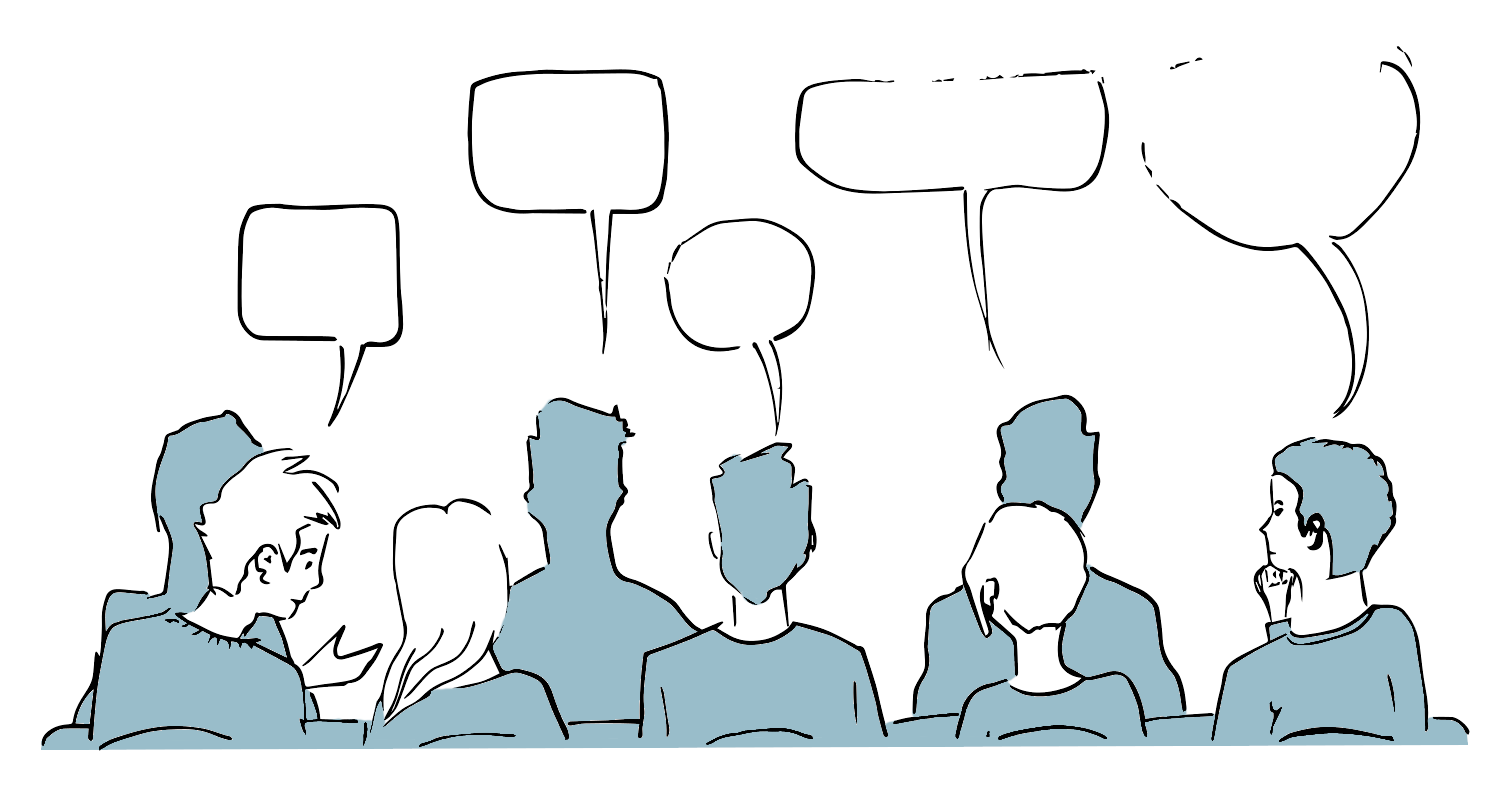
\includegraphics{Figures/14-01-Deliberation} \end{center}

\section{Digitale Technologien als Gegenstand von Unterricht -- Einsatzpunkte und Fragestellungen}\label{digitale-technologien-als-gegenstand-von-unterricht-einsatzpunkte-und-fragestellungen}

Im Sinne eines epochaltypischen Schlüsselproblems markiert die Digitalisierung keinen fixen Zustand, sondern ein ergebnisoffenes Problem- und Handlungsfeld, das gesellschaftlicher Aushandlungen wie auch individueller Positionsbestimmungen bedarf. Aus dieser Perspektive verbergen sich hinter vielen der postulierten Kompetenzen weiterreichende Fragestellungen, wie an den folgenden einigen Beispielen aufgezeigt werden soll:

{\emph{2.4.1 Die Schülerinnen und Schüler können um Regeln der Online-Kommunikation wissen und diese beachten. Sie können die Verhaltensregeln der realen und der virtuellen Welt in Beziehung setzen und diese gleichermaßen beachten.}}

Kommunikations- und Verhaltensregeln erscheinen in dieser Darstellung als objektive Größen, die es zu beachten gelte. Offen bleibt jedoch die Frage, woher diese Regeln eigentlich kommen und woher sie ihre normative Kraft beziehen. Inwiefern sind entsprechende Regeln universell gültig oder doch kulturell geprägt? Basieren sie auf dem Konsens der Nutzer*innen, staatlichen Vorgaben oder den Ideen \& Inter-essen der Unternehmen, die die jeweiligen Plattformen betreiben?

{\emph{3.3. Die Schülerinnen und Schüler können Chancen und Risiken sowie rechtliche Grundlagen im Umgang mit Medien/ medialen Angeboten analysieren und berücksichtigen (z.B. Datenschutz, Datensicherheit, Urheberrecht, Lizenzrecht).}}

Die Chancen, Risiken und rechtlichen Grundlagen erscheinen hier als fixe Größen, die es zu berücksichtigen gelte. Ausgeklammert wird in dieser Perspektive jedoch das gesellschaftliche Ringen um eben jene rechtlichen Grundlagen. Standards zum Datenschutz und zur Datensicherheit mussten kollektiv errungen werden und sind immer noch Gegenstand kontroverser Debatten hinsichtlich ihrer Auslegung. Ebenso verhält es sich mit der Frage, ob das gegenwärtige Urheber- und Lizenzrecht den Bedingungen einer digitalisierten Gesellschaft angemessen ist und wessen Interessen es dient.

{\emph{5.5.2 Die Schülerinnen und Schüler können abschätzen, welche Abläufe sich für eine Automatisierung eignen.}}

Auch hier entsteht der Eindruck, dass sich eindeutig bestimmen ließe, welche Abläufe sich für eine Automatisierung eignen. Die Frage danach, welche Abläufe sich zur Automatisierung eigenen, beruht aber nicht zuletzt auf unseren gesellschaftlichen Vorstellungen bezüglich der Regelhaftigkeit der zu automatisierenden Vorgänge \citep{heintzHerrschaftRegelZur1993}. Ob wir davon ausgehen, dass sich Autos selbständig im Verkehr bewegen, die Erfolgsaussichten einer Person in einem bestimmten Ausbildungsberuf vorausberechnet werden oder Emotionen mittels Künstlicher Intelligenz erkannt werden können, basiert immer auch auf unseren Vorstellungen über uns selbst und ist insofern niemals eine rein technische Frage.

{\emph{6.2.5 Die Schülerinnen und Schüler können die Bedeutung digitaler Medien für die politische Meinungsbildung und Entscheidungsfindung benennen.}}

Die Beschreibung legt nahe, dass es eindeutige Modelle zur Analyse des Medieneinflusses auf die politische Meinungsbildung gäbe. Gerade im Zuge der Digitalisierung sehen wir jedoch, dass sich die Formen der Meinungsbildung ebenfalls wandeln. Von Influencern über Bot-Armeen und Fake-News bis hin zur Bildung von Filterblasen und Echokammern sind wir mit einer Vielzahl neuer Formen und Mechanismen der Meinungsbildung konfrontiert, ohne dass wir ein gefestigtes Wissen über Ausmaß und genaue Wirkung hätten.

\section{Zum Umgang mit Digitalen Technologien im Unterricht - Fragen von Macht, Mitbestimmung und Teilhabe}\label{zum-umgang-mit-digitalen-technologien-im-unterricht---fragen-von-macht-mitbestimmung-und-teilhabe}

Jenseits der Auseinandersetzung mit Aspekten der Digitalisierung als Gegenstand von Unterricht stellen sich aus einer kulturtheoretischen Perspektive aber auch Fragen von Macht, Mitbestimmung und Teilhabe beim Einsatz und Umgang mit digitalen Technologien im Unterricht. Dies gilt insbesondere dann, wenn der Lern- und Bildungsort Schule eine »verantwortliche, auf demokratischem Grundverständnis basierende Mitgestaltung und Auseinandersetzung mit den kontinuierlich entstehenden neuen Inhalten und Strukturen« \citep[S. 4]{ministeriumfurbildungwissenschaftundkulturdeslandesschleswig-holsteinErganzungenFachanforderungenMedienkompetenz2018} befördern will.

{\emph{2.5.1 Die Schülerinnen und Schüler können sich aktiv in virtuellen Räumen beteiligen und als selbstbestimmte Bürgerin/selbstbestimmter Bürger agieren (z.B. E-Government, Online-Banking, Online-Shopping).}}

Welche konkreten Möglichkeiten bieten sich den Schüler*innen, im Kontext von Schule und Unterricht in die Rolle selbstbestimmter Bürger*innen hineinzuwachsen und zum Beispiel darüber mitzubestimmen, welche Daten über ihr digitales Lernverhalten gesammelt, analysiert und zur Grundlage von Entscheidungen gemacht werden, die den ihren individuellen Bildungsweg beeinflussen können?

{\emph{5.4.1 Die Schülerinnen und Schüler können zur Unterstützung des schulischen Lernens geeignete Online-Lernumgebungen identifizieren, erproben und zur Wissensaneignung, -generierung oder Zusammenarbeit nutzen.}}

Auch hier stellt sich die Frage nach der praktischen Umsetzung im Kontext von Schule und Unterricht. Wie und in welchem Ausmaß werden die Schüler*innen in die Identifikation, Auswahl und Erprobung digitaler (Lern-)Technologien im Schulalltag tatsächlich mit einbezogen? Wie können sie diese Kompetenz erwerben und von ihr Gebrauch machen, wenn sie z.B. ihr Smartphone nicht im Unterricht benutzen dürfen? Wer bestimmt darüber, ob die Suche nach Informationen in der Wikipedia, eine Anfrage in einem Expertenforum, oder die Verwendung von Anwendungen wie ChatGPT als ›geeignet‹ zu betrachten ist?

{\emph{6.2.5 Die Schülerinnen und Schüler können sich reflektiert mithilfe von Kommunikationsmedien an politischen Entscheidungs- und Meinungsbildungen beteiligen (z. B. Online-Petition).}}

Auch an dieser Stelle kann die Schule als ein besonderes Lernfeld für die Schüler*innen fungieren, in dem sich, auch unterstützt von digitalen Systemen wie beispielsweise \href{https://www.aula.de/}{›Aula‹}, Schüler*innen die Möglichkeit bietet, sich aktiv an der politischen Entscheidungs- und Meinungsbildung im Kontext der Schule zu beteiligen.

{\emph{6.2.6 Die Schülerinnen und Schüler können Potenziale der Digitalisierung im Sinne sozialer Integration und Teilhabe erkennen und diese detailliert analysieren.}}

Neben den Potenzialen der Digitalisierung im Sinne sozialer Integration und Teilhabe sind unter dem Schlagwort der digitalen Spaltung vielfältige Formen der Desintegration und digitaler Bildungsungleichheiten in der Literatur beschrieben und empirisch belegt worden \citep{kutscherDiskussionsfelderMedienpaedagogikMedien2021, verstandigZeroLevelDigitalDivide2016}. Hieraus ergibt sich die Frage, ob der Einsatz konkreter Technologien tatsächlich den unterschiedlichen Erfahrungen und Möglichkeiten aller betroffenen Schüler*innen gerecht wird, oder ob er bestehende Ungleichheiten verstärkt oder neue schafft.

\begin{blackbox}
\emph{Wie lassen sich Fragen der Digitalisierung als einem epochaltypischen Schlüsselproblem im Rahmen des Fachunterrichts thematisieren?}

\end{blackbox}

~

\begin{blackbox}
\emph{Wie könnten Möglichkeiten der Mitbestimmung und Teilhabe von Schüler*innen bezüglich des Einsatzes und des Umgangs mit digitalen Technologien in Ihrem Unterricht aussehen?}

\end{blackbox}

\section{Partizipationsorientierter Technikeinsatz}\label{partizipationsorientierter-technikeinsatz}

\emph{(Autor*innen: Isabelle Simon \& Christoph Richter, 2023)}

\textbf{Ziel}

Der partizipationsorientierte Technikeinsatz
dient der Identifikation von Mitbestimmungs- und Gestaltungsmöglichkeiten bei der Nutzung digitaler Technologien in institutionellen Kontexten.

\textbf{Leitgedanke}

Insbesondere in institutionellen Kontexten, wie der Schule, erfolgen Entscheidungen über die Auswahl und den Umgang mit digitalen Technologien oftmals ohne die direkte Einbindung aller Nutzer*innen, wie etwa den Schüler*innen. Vor dem Hintergrund einer digitalen Medienbildung, die zu einer demokratischen Mitbestimmung und Mitgestaltung im Kontext der Digitalisierung befähigen soll, erscheint es deshalb notwendig, die mit dem Einsatz digitaler Technologien verbundenen Möglichkeiten einer partizipativen Teilhabe systematisch zu erkunden und umzusetzen. Ein solcher Schritt impliziert dabei immer auch eine Sensibilisierung für die in institutionellen Kontexten implizierten Machtverhältnisse, sowie eine möglichst umfassende Betrachtung der mit dem Einsatz digitaler Technologien verbundenen Formen der In- und Exklusion bestimmter Erfahrungs- und Handlungsmöglichkeiten für die verschiedenen Personengruppen.

\textbf{Anwendungskontext}

Der Anwendungsbereich umfasst alle Phasen des Technikeinsatzes, von der Auswahl- und Einführung über die Nutzung bis hin zur Nachnutzung.

\begin{center}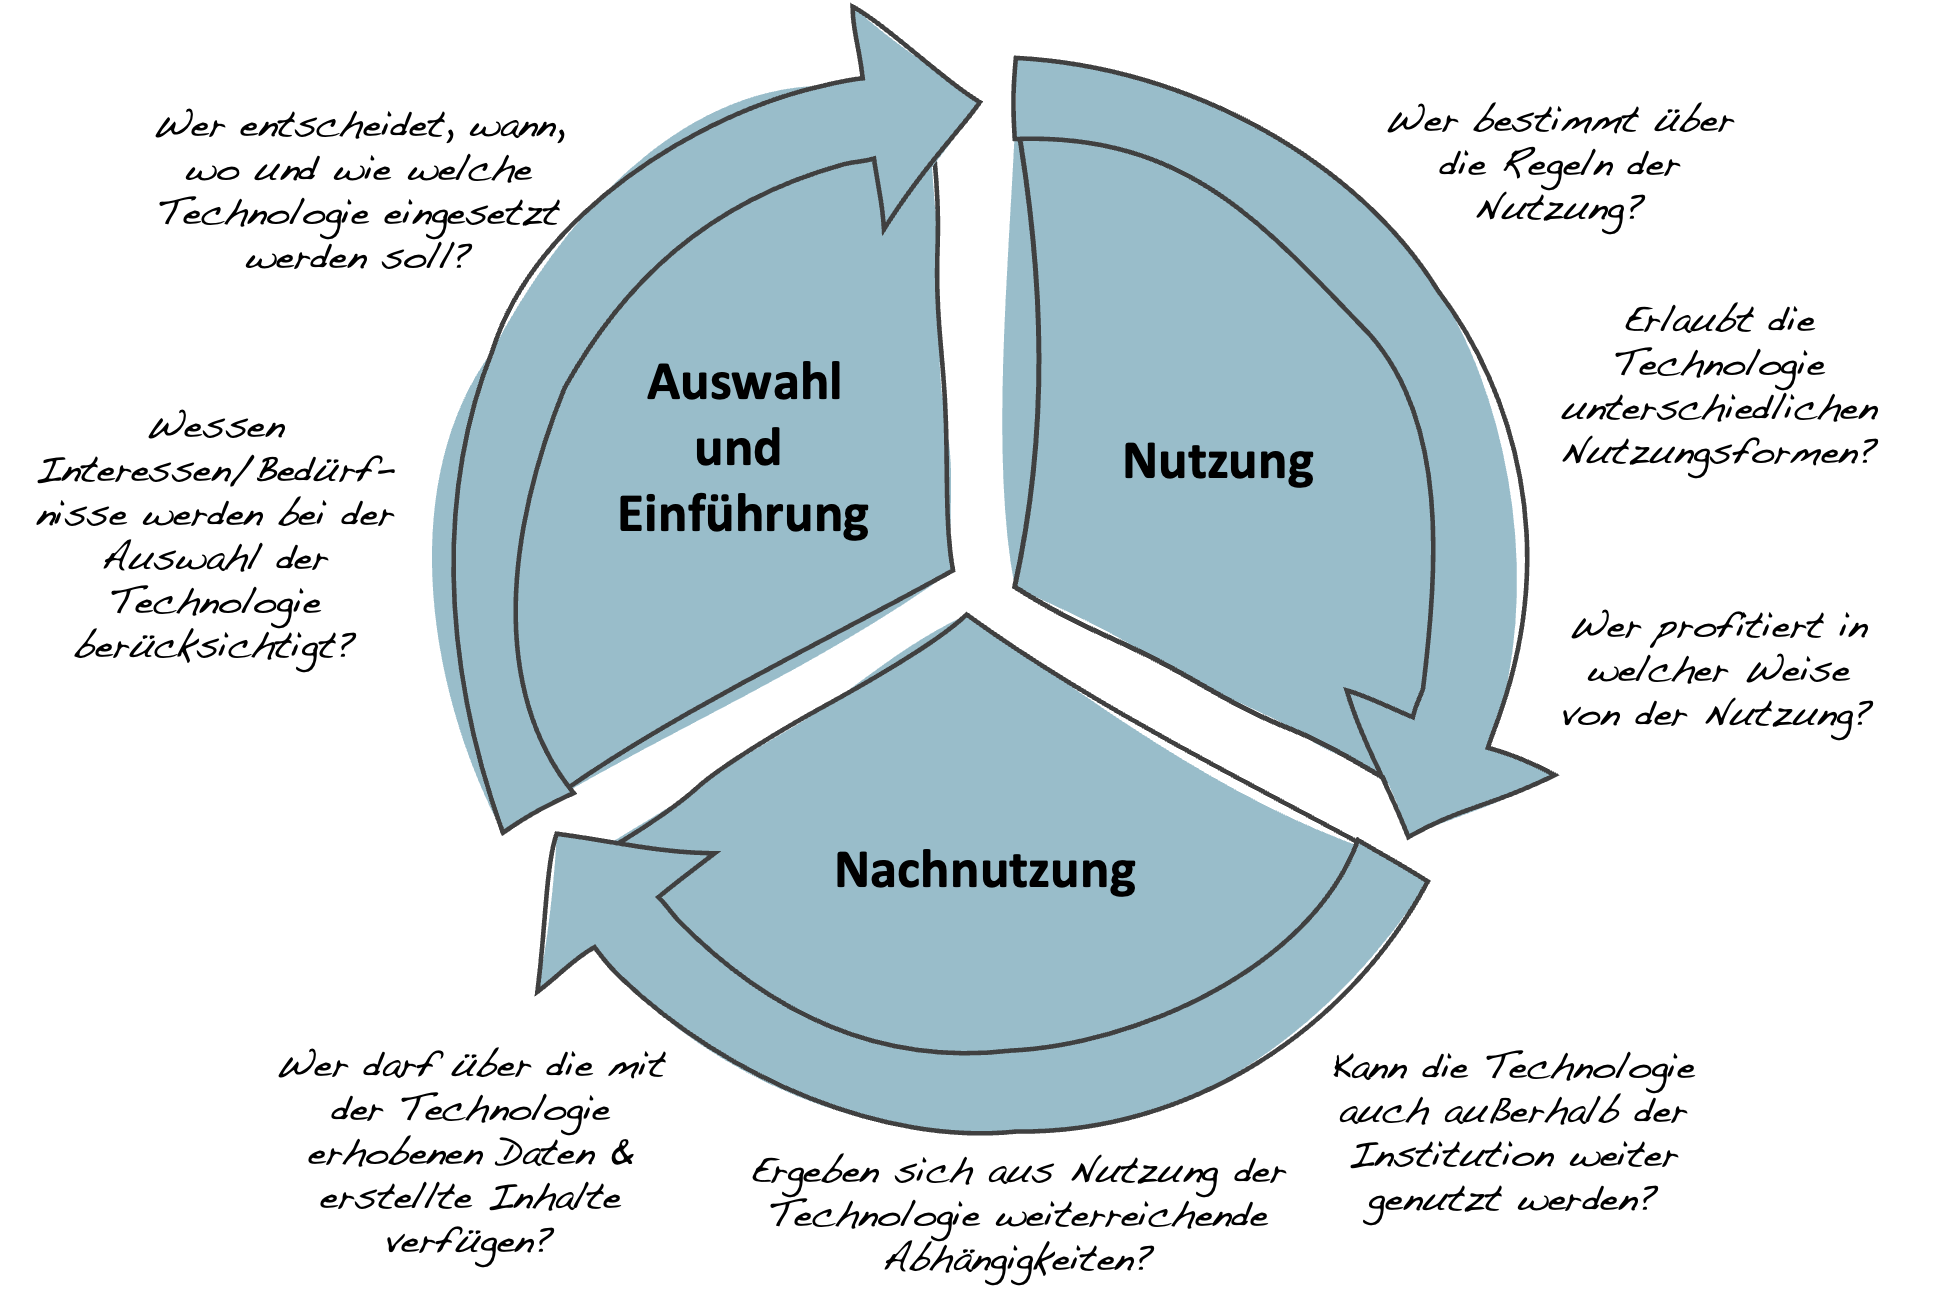
\includegraphics{Figures/14-02-PartTechnik} \end{center}

\textbf{Arbeitsschritte}

\begin{enumerate}
\def\labelenumi{\arabic{enumi}.}
\tightlist
\item
  Identifikation der von dem Technikeinsatz betroffenen Personengruppen.
\item
  Klärung der vorhandenen Gestaltungs- und Entscheidungsspielräume.
\item
  Einladung der betroffenen Personengruppen zur Mitbestimmung und -gestaltung.
\item
  Gemeinsame Exploration realisierbarer Optionen.
\item
  Aushandeln einer verbindlichen Entscheidung.
\item
  Umsetzung und gemeinsame Evaluation der Entscheidung.
\end{enumerate}

\textbf{Ergebnisformat}

Gemeinsam getragene Entscheidungen zum Einsatz digitaler Technologien unter Berücksichtigung der Interessen aller Betroffenen.

\textbf{Praktische Tipps}

\begin{itemize}
\tightlist
\item
  Die vorhandenen Gestaltungs- und Entscheidungsspielräume sollten möglichst klar umschrieben werden, um den Prozess zu fokussieren und irreführende Erwartungen zu vermeiden.
\item
  Bei der Planung eines partizipativen Entscheidungs- bzw. Gestaltungsprozesses sind sowohl die Bereitschaft der Betroffenen wie auch ihre Vorerfahrungen und Kompetenzen mit zu berücksichtigen.
\item
  Für den Partizipationsprozess sollte ein ausreichender Zeitrahmen eingeplant werden, damit sich alle Betroffenen einbringen können und Gehör finden.
\end{itemize}

\textbf{»Fallstricke«}

\begin{itemize}
\tightlist
\item
  Ein partizipatives Vorgehen bedeutet nicht, dass allen Ideen und Wünschen Rechnung getragen werden kann oder sollte. Ziel ist vielmehr die Aushandlung tragfähiger Entscheidungen unter der Prämisse eines demokratischen und solidarischen Miteinanders.
\item
  Ein partizipatives Vorgehen ist nicht geeignet, wenn keine realen Möglichkeiten zur Mitentscheidung und --gestaltung bestehen. Dies gilt insbesondere dann, wenn ein partizipatives Vorgehen nur dazu dienen soll, bereits getroffene Entscheidungen zu legitimieren.
\end{itemize}

\begin{licencebox}{licencebox}
Der Leittext ›Partizipationsorientierter Technikeinsatz‹ wurde 2023 von Isabelle Simon und \href{mailto:richter@paedagogik.uni-kiel.de}{Christoph Richter} erstellt und ist unter einer Creative Commons \href{https://creativecommons.org/licenses/by-sa/4.0/}{CC BY-SA 4.0} Lizenz veröffentlicht.

\end{licencebox}

\chapter*{Anhang}\label{anhang}
\addcontentsline{toc}{chapter}{Anhang}

Die beiden folgenden Beispiele wurden von Helena Hintz und Jamila Becker erstellt. Sie setzen sich anhand der minimalen Leitexte mit dem digitalen ›Referatedienst‹ Blinkist sowie mit der Verwendung von WhatsApp zur Gruppenarbeit im Studium auseinander.

Die Beispiele sollen mögliche Zugänge zur eigenen Auseinandersetzung mit digitalen Technologien und den mit ihnen verbundenen Praktiken aufzeigen. Darüber hinaus können die Reflexionen der Autorinnen als Einsatzpunkte für weiterführende Diskussionen genutzt werden. Die Beispiele erheben keinen Anspruch auf Vollständigkeiten, sondern markieren vielmehr Durchgangspunkte in den Auseinandersetzungen ihrer Autorinnen.

\section*{Beispiel Blinkist}\label{beispiel-blinkist}
\addcontentsline{toc}{section}{Beispiel Blinkist}

\begin{licencebox}{licencebox}
Das Beispiel ›Blinkist‹ wurde 2022 von \href{mailto:hel.hintz@gmail.com}{Helena Hintz} erstellt und ist unter einer Creative Commons \href{https://creativecommons.org/licenses/by-sa/4.0/}{CC BY-SA 4.0} Lizenz veröffentlicht.

\end{licencebox}

\subsection*{Kartierung sozialer Praktiken (Kapitel 5)}\label{kartierung-sozialer-praktiken-kapitel-5}
\addcontentsline{toc}{subsection}{Kartierung sozialer Praktiken (Kapitel 5)}

\begin{center}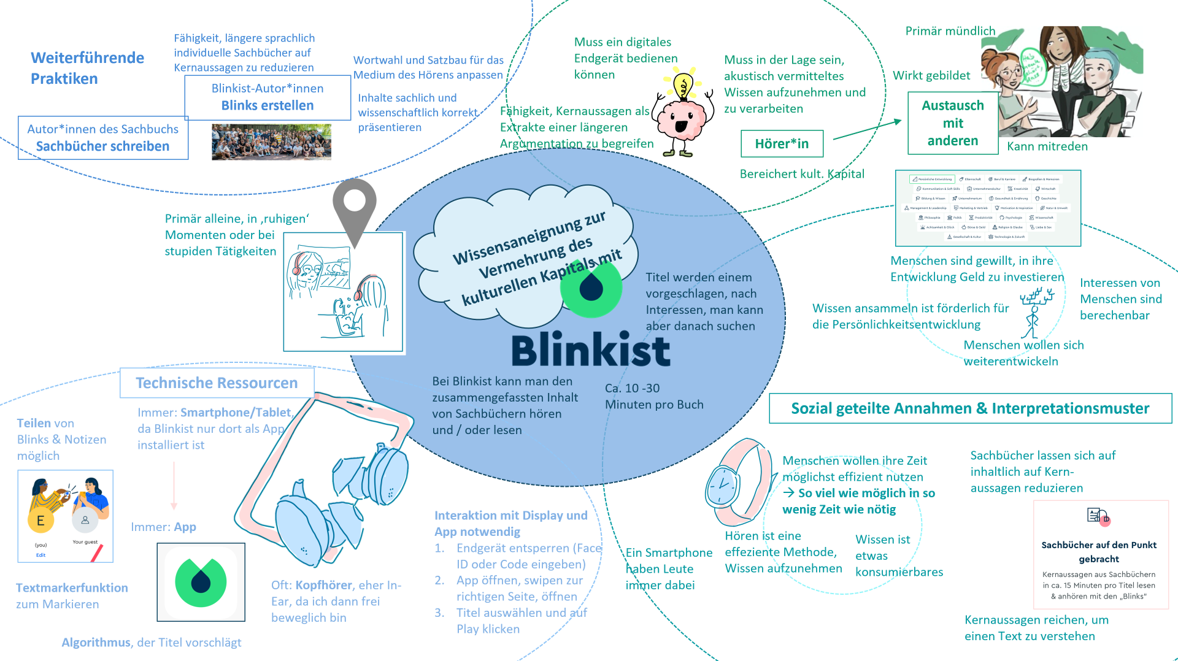
\includegraphics{Figures/05-Bsp.-Blinkist} \end{center}

\textbf{Reflexion}

Bezüglich der technischen Ressourcen fand ich sehr spannend, dass meine Praxis mit einem digitalen mobilen Endgerät und der darauf installierten App Blinkist eng verzahnt ist (in meinem Fall mein Smartphone), ohne welches ich keine Blinks hören kann. Im Gegensatz zu einem Sachbuch (das wäre in meinem Fall das Äquivalent zu Blinks) muss ich nicht nur in der Lage sein, mir ein Buch zu beschaffen und lesen zu können, sondern auch dazu fähig sein, ein digitales Gerät zu bedienen etc.
In Hinblick auf sozial geteilte Annahmen und Interpretationsmuster sind mir primär zwei Punkte besonders aufgefallen.

Zum Ersten unterwirft sich das Modell von Blinkist durch seine auf Minuten verkürzten Buchthesen einem gesellschaftlichen Konsum-System, in welchem davon ausgegangen wird, dass ich als Nutzerin so viel wie möglich in so wenig Zeit wie nötig zu mir nehmen möchte. Wissen wird konsumierbar, was für mich in ein System passt, das Schüler*innen in immer kürzerer Zeit immer mehr Stoff vermitteln möchte. Zeit für Auseinandersetzung mit den Inhalten, ein Innehalten zwischen Buchseiten oder Kapiteln, wie ich es mir beim Lesen erlaube, fällt weg.
Stattdessen kann ich jetzt abwaschen UND mir Wissen aneignen gleichzeitig.

Eine zweite entscheidende Erkenntnis, die sich aus der Auseinandersetzung ergibt, und auf die ich im Abschnitt zur Rekonstruktion operationaler Formen zurückkommen werde, ist die Annahme, dass Sachbücher sich inhaltlich auf Kernaussagen reduzieren lassen. Bei der ‚Umwandlung` in Blinks entstehen völlig neue Texte, die sprachlich mit dem Original wenig zu tun haben. Die Blinks nutzen als optische Anker trotzdem die Cover des Buches. Aus literarischer und linguistischer Perspektive stellen sich für mich die Fragen: Wann ist ein Text ein Text? Wie definiert sich Autorschaft? Was macht es mit einem Text, wenn man nur mit seinem Inhalt arbeitet?

\subsection*{Szenarien (Kapitel 7)}\label{szenarien-kapitel-7}
\addcontentsline{toc}{subsection}{Szenarien (Kapitel 7)}

\textbf{Szenario 1: Wissensaneignung heute}

\begin{center}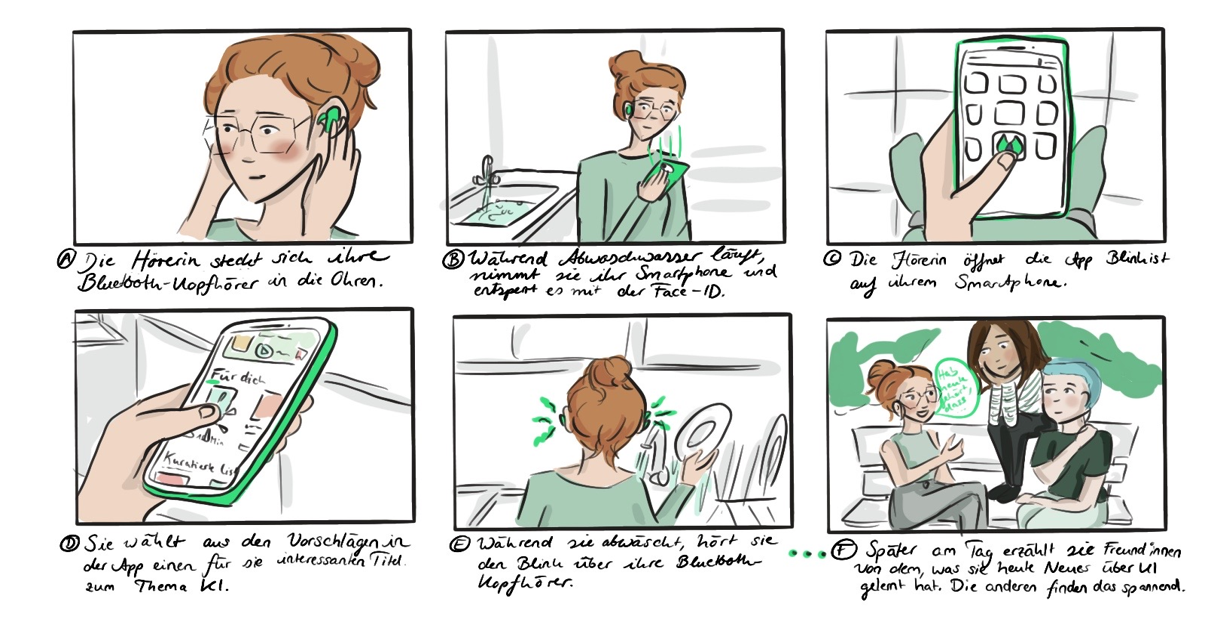
\includegraphics{Figures/07-Bsp.-Szenario1} \end{center}

\textbf{Szenario 2: Wissensaneignung früher}

\begin{center}\includegraphics{Figures/07-Bsp.-Szenario2} \end{center}

\textbf{Reflexion}

Ich habe die Wissensaneignung mit Blinkist zur Vermehrung meines kulturellen Kapitals mit einem fiktiven vor-digitalen Szenario verglichen. Die zwei großen Unterschiede lagen hierbei in der Form der Aneignung (hören vs.~lesen) sowie in der Form der Kommunikation meines neu erworbenen Wissens.

{\textbf{a) Form der Aneignung}}

Blinkist ist praktisch. Ich wähle einen Blink zu einem Thema, das mich interessiert, stecke mir meine Kopfhörer in die Ohren, drücke auf meinem Smartphone auf Play und mache den Abwasch, während mir in 15 Minuten die wichtigsten Thesen eines Sachbuchs zusammengefasst werden. Der Abwasch ist zu Ende. Der Blink ist zu Ende. Ich habe etwas erledigt und etwas gelernt. Check.

Wie hätte ich mir in kurzer Zeit Wissen angeeignet, bevor es sowas wie Blinkist auf dem Markt gab? Da gab es natürlich verschiedene Möglichkeiten, in diesem Beispiel habe ich mich für die Nutzung eines Konversationslexikons entschieden. Das sind Nachschlagewerke, die Wissen möglichst verständlich und umfassend darstellen. Erstmal musste ich natürlich irgendwo hingehen und mir einen der Bände des Konversationslexikons aussuchen mit einem Thema, das mich interessierte. Wenn ich dann das Buch hatte, musste ich irgendwo hingehen und darin den Text zu dem Thema meiner Wahl lesen. Dabei konnte ich nichts nebenbei machen, aber dafür vielleicht weiterblättern und mich zu anderen Themen treiben lassen. Das geht bei Blinkist durch Vorschläge natürlich auch, aber kurz einen Text überfliegen geht nur im Lexikon. Ein Punkt, der das Lexikon problematisch macht, ist, dass die einzelnen Beiträge, besonders in Hinblick auf bestimmte Themen, ideologisch gefärbt sein konnten. Ohne weitere Quellen miteinzubeziehen, könnten manche Definition und Erläuterungen damit sehr problematisch sein. Bei Blinkist habe ich die Möglichkeit, die Namen der Original-Autor*innen einzusehen und über eine Suchmaschine mehr über dieselben herauszufinden.

{\textbf{b) Kommunikation}}

In meinem Blinkist-Szenario erzähle ich zwei Freund*innen von meinem neuen Wissen über KI, welches ich mir über Blinkist erworben habe. Ich schreibe, dass sie es spannend finden. Da sie selber auch Teil einer Welt sind, in denen jede Information nur einen Klick mit dem Finger entfernt ist, sind sie aber auch nicht beeindruckt, sondern stellen vielleicht selber kritische Fragen. Falls sie Nachfragen zum Buch haben, kann ich nicht wirklich darauf eingehen. Ob mir das Buch gefallen hat? Keine Ahnung, aber die Thesen fand ich spannend.

In meinem Konversationslexikons-Szenario sind meine Freund*innen etwas beeindruckter. Ich habe mir Wissen angeeignet in einer Zeit, in der meine Aussagen nicht mittels einer Google-Suchanfrage negiert oder bestätigt werden können. Ich stelle mir vor, dass ich mit meinem Wissen aus einem dicken Buch ernst genommen werde, schließlich war ich ja extra in der Bibliothek, statt nur jemand anderen zu fragen oder ähnliches.

Das Ganze ist mit einem Augenzwinkern gemeint, aber ich möchte damit darauf anspielen, dass Sachwissen heutzutage zugänglicher ist denn je. Natürlich ist es heute auch umso schwieriger, die Seriosität von Quellen zu beurteilen und zu bewerten, wie relevant welche Information ist. Man hat ständig das Gefühl, jedes neue Wissen ins Verhältnis zu anderem zu setzen. Ich stelle mir vor, dass das vor der Dominanz der Internets anders war. Dass man Wissen aus einem Buch mehr angenommen hat, statt es in zwanzig Foren mit anderen Aussagen zu vergleichen.

\subsection*{Rekonstruktion der Produktvision (Kapitel 8)}\label{rekonstruktion-der-produktvision-kapitel-8}
\addcontentsline{toc}{subsection}{Rekonstruktion der Produktvision (Kapitel 8)}

\begin{center}\includegraphics{Figures/08-Bsp.1} \end{center}

\textbf{Reflexion}

Blinkist macht es einem recht leicht, wenn man versucht, die Produktvision nachzuvollziehen. Ich habe als Slogan für das Produkt „Mehr Wissen in weniger Zeit`` gewählt, um die Idee der Effizienz der Anwendung aufzugreifen. Meine Produktverpackung soll die potentielle Zielgruppe vielbeschäftigter, in sich selbst investierender Bürger*innen ansprechen, eben „Alle, die viel wissen wollen, aber wenig Zeit haben``.

Bei der Auseinandersetzung mit der Produktvision wurde mir dieser Aspekt der Effizienz besonders bewusst. Die Gestaltung des Interfaces und der Werbung für die App, die ich in meiner Produktvision rekonstruiere, machen diesen Gedanken zu etwas Attraktivem, vielleicht sogar Hilfreichem. Dass man für die Nutzung der App Geld bezahlt, wird zu Beginn nicht kommuniziert, erst wird ein nützliches Lifestyle-Produkt vermarktet. Das hat mir gezeigt, wie die Ästhetisierung von einer Applikation zu deren Vermarktung beitragen kann. Einem wird vermittelt, dass man mit der App etwas ‚für sich tut`, womit Blinkist sich letztendlich mit anderen Konsumgütern gleichstellt. Mit der Bewerbung von Büchern ist das nicht vergleichbar.

\subsection*{Rekonstruktion operationaler Formen (Kapitel 9)}\label{rekonstruktion-operationaler-formen-kapitel-9}
\addcontentsline{toc}{subsection}{Rekonstruktion operationaler Formen (Kapitel 9)}

\begin{center}\includegraphics{Figures/09-Bsp.1} \end{center}

\textbf{Reflexion}

Die Rekonstruktion der operationalen Formen fiel mir erst ziemlich schwer, aber die Auseinandersetzung mit der Kartierung der Benutzungsflüsse hat dabei geholfen, einen Zugang zu den von der Applikation vorgeschlagenen Handlungsoptionen zu erhalten. Ich war überrascht, wie simpel sich die Flüsse ausgestalten. Spannend fand ich weiterhin, dass es immer wieder Feedbackschleifen gibt, bspw. wenn ein gesuchter Titel nicht gefunden wird, kann immer wieder auf die angebotenen Optionen der App zurückgegriffen werden. Die Entwickler*innen der App scheinen gut vorgesorgt zu haben, dass Nutzer*innen möglichst bei jedem Öffnen dazu kommen, einen Blink anzuhören, indem das Nichtfinden eines Blinks einen zu neuen Vorschlägen weiterleitet, die man entweder in Anspruch nehmen kann oder eben zurück zur Startseite kehrt. Ich glaube, es war am schwierigsten für mich, mich von der Perspektiv der Nutzerin zu lösen und wirklich darauf zu gucken, was genau in der Anwendung passiert und was diese vorgibt.

Um es gut nachzuzeichnen, muss man das menschliche Denken wirklich verlassen und schauen, was auf eine Interaktion mit der Anwendung wirklich folgt. Das fand ich sehr anspruchsvoll, hat mir aber auch Unterschiede zwischen meinem Denken und der Konstruktion der Abläufe verdeutlicht.

\subsection*{Anwendungsbezogene Datenkritik (Kapitel 10)}\label{anwendungsbezogene-datenkritik-kapitel-10}
\addcontentsline{toc}{subsection}{Anwendungsbezogene Datenkritik (Kapitel 10)}

\begin{center}\includegraphics{Figures/10-Bsp.1} \end{center}

\textbf{Reflexion}

In der Datenkritik empfinde ich vor allem die operationale Rekonstruktion und die Formalisierung als spannend. Dass bei Blinkist Sachbuchtexte mit einem eigenen sprachlichen Stil auf ihre Kernthesen reduziert werden und damit eine Objektivierbarkeit dieser Werke impliziert wird, indem der Text auf eine ‚richtige Lesart` reduziert wird, empfinde ich als problematisch. Ich frage mich, ob es überhaupt möglich ist, einen nicht-wissenschaftlichen Text derart zu reduzieren, ohne ihn dabei zu verlieren? Blinkist beschreibt Blinks als eigene Werke, wodurch eine Distanzierung zum Original stattfindet, aber sie werben mit den Covern der Bücher, als würde man das Originalwerk einfach in verkürzter Form kriegen. Dabei folgt die Formalisierung einem scheinbar festen Konzept von Blinkist.

Es wird eine verschriftlichte Struktur erstellt, die die „Schlüsselideen``, also die Kernthesen, verdeutlicht. Jedes Buch erhält dabei eine eigene Struktur. Was bleibt hierbei über vom Text? Kann ich mich als Hörerin darauf verlassen, dass der Inhalt des Textes ‚richtig verstanden` und ‚richtig wiedergegeben` wurde? Vielleicht hätte ich das Original anders aufgefasst. Die entstandenen neuen Strukturen werden eingelesen und in Audiodateien umgewandelt. Der Gegenstand wird zum Blink und kann angehört werden. Er wird auf seinen Informationsgehalt reduziert wahrgenommen und vermutlich dahingehend bewertet, wie nachvollziehbar die Thesen dargestellt werden. So kann ein 528 seitiges Buch auf 11 Kernaussagen reduziert angehört werden.

\subsection*{Kartierung von Benutzungsflüssen (Kapitel 11)}\label{kartierung-von-benutzungsfluxfcssen-kapitel-11}
\addcontentsline{toc}{subsection}{Kartierung von Benutzungsflüssen (Kapitel 11)}

\begin{center}\includegraphics{Figures/11-Bsp.1} \end{center}

\textbf{Reflexion}

Ich fand es spannend, mir mit der Kartierung der Benutzungsflüsse bewusst zu machen, welche Angebote mir das Interface der App Blinkist macht, sobald ich mich für eine der angebotenen Handlungsoptionen entscheide. Ich tippe beispielsweise auf das Icon für ‚Suchen` und habe dann durch das Interface das Angebot, einen Titel, Autor oder Stichwort in die Suchleiste einzutippen oder einen Vorschlag auszuwählen, den ich durch weiteres Tippen noch im Format eingrenzen kann. Bevor ich die Benutzungsflüsse kartiert habe, war mir nicht bewusst, wie sehr die Gestaltung einer Applikation meinen Umgang mit derselben steuert. Dadurch, dass mir verschiedene Handlungsoptionen zur Verfügung gestellt werden, entsteht bei mir ein Gefühl der mehr oder weniger eingeschränkten Wahlfreiheit in meinem Umgang (hier wäre beispielsweise eine Beschränkung auf das Hören eines Audioformats gegeben, ich habe in der Anwendung nicht die Option, gebrauchte Möbel zu kaufen). Dass aber eigentlich die App meinen Benutzungsfluss ‚bestimmt`, indem sie diejenige ist, die mir Optionen anbietet, wird aber erst in dieser ausdifferenzierten Betrachtung des Prozesses bewusst. Spannend finde ich noch, dass das Hören selber außerhalb der Nutzung des Smartphones stattfindet. Zwar läuft der Sound natürlich über die Applikation, aber ich kann das Smartphone aus der Hand legen und mich in der außerdigitalen Welt bewegen und dort handeln, während ich den Blink höre.

\subsection*{Kartierung des technischen Milieus (Kapitel 12)}\label{kartierung-des-technischen-milieus-kapitel-12}
\addcontentsline{toc}{subsection}{Kartierung des technischen Milieus (Kapitel 12)}

\begin{center}\includegraphics{Figures/12-Bsp.1} \end{center}

\textbf{Reflexion}

Aus der Kartierung soziotechnischer Milieus nehme ich vor allem mit, dass Blinkist einige sozial geteilte Handlungs- und Deutungsmuster voraussetzt, die vor allem stark an das sozioökonomische System der ständigen Selbstoptimierung gekoppelt sind. Mehr Wissen in weniger Zeit -- das setzt voraus, dass ich dieses Ziel als erstrebenswert erachte. Ich erachte es als erstrebenswert in einer Gesellschaft, in der ich wenig Zeit habe, aber viel Wissen als hohes Gut angesehen wird. Die Standards und Protokolle, die hinter der Entstehung von Blinks stehen, finde ich dabei nicht transparent. Bei der Datenkritik lässt sich zwar nachvollziehen, wie Blinks generell entstehen, allerdings ist meine Annahme, dass jeder Vorgang immer individuell an das Werk angepasst werden muss, da diese unterschiedlich komplex sind. Bezüglich meiner mit Blinks verbundenen Praktik, der Bereicherung des kulturellen Kapitals, sehe ich mittlerweile ein deutliches Zusammenwirken mit dem System der Wissensgesellschaft. Statt in die Tiefe zu gehen, mich mit einzelnen Sätzen und Gedanken auseinanderzusetzen, wie einem Buch, ermöglicht Blinkist mir, viel aufzunehmen, mir viel Wissen anzueignen, es zu konsumieren. Damit scheint Blinkist gut auf den Markt zu passen, gut in unser Bildungssystem zu passen und ich glaube, dass man diese Anwendung gut für sich nutzen kann, aber reflektieren sollte, was dahinter steht. Die Auseinandersetzung hat mir gezeigt, wie wichtig es ist, sich mit den Praktiken, die mit einer Anwendung verbunden sind, kritisch-reflektierend auseinanderzusetzen. Hinter attraktiven Interfaces und meinem Umgang mit diesen versteckt sich oft viel mehr, als auf den ersten Blick sichtbar ist.

\section*{Beispiel WhatsApp}\label{beispiel-whatsapp}
\addcontentsline{toc}{section}{Beispiel WhatsApp}

\begin{licencebox}{licencebox}
Das Beispiel ›Blinkist‹ wurde 2022 von Jamila Becker erstellt und ist unter einer Creative Commons \href{https://creativecommons.org/licenses/by-sa/4.0/}{CC BY-SA 4.0} Lizenz veröffentlicht.

\end{licencebox}

\subsection*{Kartierung sozialer Praktiken (Kapitel 5)}\label{kartierung-sozialer-praktiken-kapitel-5-1}
\addcontentsline{toc}{subsection}{Kartierung sozialer Praktiken (Kapitel 5)}

\begin{center}\includegraphics{Figures/05-Bsp.-Whatsapp} \end{center}

\textbf{Reflexion}

Die Voraussetzungen für eine soziale Praxis, die eine Technologie integriert/beinhaltet/über diese praktiziert wird/etc., sind viel mehr als nur das Verfügen über diese Technologie. Zwar ist die Technologie als solche elementar, jedoch funktioniert die Praxis nicht ohne entsprechende Fertigkeiten bzw. Kenntnisse und vor allem die sozial geteilten Interpretationsmuster. Ohne die entsprechenden geteilten Vorstellungen, die Bereitschaft, die Technologie zu integrieren, kann eine Technologie keine soziale Praxis ändern. Dies bedeutet ggf. auch eigene Vorstellungen oder Moral zu verändern. So müssen sich zum Beispiel nicht nur alle damit einverstanden erklären, die Gruppenarbeit über WhatsApp stattfinden zu lassen sondern sich auch auf die sozial geteilten Interpretationsmuster wie ständige Verfügbarkeit und Verzicht auf engeren sozialen Kontakt bei der Gruppenarbeit einlassen.

\subsection*{Szenarien (Kapitel 7)}\label{szenarien-kapitel-7-1}
\addcontentsline{toc}{subsection}{Szenarien (Kapitel 7)}

\textbf{Szenario 1: Gruppenarbeit in Präsenz (eigene Erfahrungen)}*

\begin{center}\includegraphics{Figures/07-Bsp.-Whatsapp1} \end{center}

{\textbf{Zoom-In 1: Treffen mit den Anderen}}

\begin{center}\includegraphics{Figures/Zoom-in1} \end{center}

\textbf{Szenario 2: Gruppenarbeit via WhatsApp (eigene Erfahrungen)}

\begin{center}\includegraphics{Figures/07-Bsp.-Whatsapp2} \end{center}

{\textbf{Zoom-In 2: Arbeitsaufteilung}}

\begin{center}\includegraphics{Figures/Zoom-in2} \end{center}

* \emph{Alle in diesem Szenario verwendeten Bilder stammen von den Bilddatenbanken \href{https://unsplash.com}{unsplash} sowie \href{https://www.pexels.com}{pexels}. Das Bildmaterial ist frei lizenziert. Nähere Informationen zu den jeweiligen Lizenzen finden sich unter \url{https://unsplash.com/de/lizenz} sowie \href{\%5Bhttps://www.pexels.com/de-de/lizenz/}{https://www.pexels.com/de-de/lizenz/}.}

\textbf{Reflexion}

Finden Gruppenarbeiten via WhatsApp statt, so führt dies nicht nur zu einer Veränderung der Arbeitsweise, die nun losgelöst ist von Raum und Zeit. Alle Beteiligten können in ihrem eigenen Tempo und mit eigenen Methoden arbeiten, sofern abgesprochene Fristen eingehalten werden. Es wird zwar ggf. ein gemeinsames Arbeitsdokument angelegt und ein Endprodukt angefertigt, jedoch ist der Arbeitsprozess unabhängig voneinander. Eine weitere massive Veränderung findet auf der sozialen Ebene statt: Es ist nicht mehr notwendig, die anderen Gruppenmitglieder kennenzulernen, es findet meist kein privater Austausch statt, die Leben der anderen bleiben unbekannt, wodurch sich der persönliche Kontakt verändern kann (weniger Verständnis, Erwartungshaltung orientiert an eigener Leistungsbereitschaft, Umgang miteinander etc.).

Auch finden weniger Diskussionen sowie Austausch über die Aufgabe und angrenzende Themen statt. Die soziale Praktik der Gruppenarbeit verändert sich durch das Medium WhatsApp massiv. Neben einer ausschließlichen Nutzung der App sind auch viele verschiedene „Hybrid-Versionen`` möglich.
Die Erstellung der Szenarien machte mir deutlich, wie stark sich eine soziale Praktik durch die Einführung einer Technologie ändern kann und wie stark auch weitere, mit der einen Praktik verbundene Praktiken, einer Veränderung unterliegen. Diese Veränderungen können je nach Standpunkt als negativ oder positiv empfunden werden.

\subsection*{Rekonstruktion der Produktvision (Kapitel 8)}\label{rekonstruktion-der-produktvision-kapitel-8-1}
\addcontentsline{toc}{subsection}{Rekonstruktion der Produktvision (Kapitel 8)}

\begin{center}\includegraphics{Figures/08-Bsp.2} \end{center}

\textbf{Reflexion}

WhatsApp ist für den privaten Gebrauch nur auf den ersten Blick kostenlos, gezahlt wird mit Daten. Dennoch nutzen sehr viele Menschen täglich den Messenger und fühlen sich mit ihm anscheinend auch sicher, die Werbekampagnen zu End-zu-End-Verschlüsselung scheinen in der Hinsicht wirksam zu sein. Überrascht hat mich, dass WhatsApp neben einem privaten Gebrauch mittlerweile auch gewerblich genutzt werden kann und hierbei auch teilweise bezahlpflichtig ist.

Die Rekonstruktion der Produktvision machte mir deutlich, wie wichtig es ist, auch hinter Werbeplakate und Selbstdarstellung zu schauen, um zu überprüfen, welche Idee hinter einem Produkt oder Unternehmen steckt.

\subsection*{Rekonstruktion operationaler Formen (Kapitel 9)}\label{rekonstruktion-operationaler-formen-kapitel-9-1}
\addcontentsline{toc}{subsection}{Rekonstruktion operationaler Formen (Kapitel 9)}

\begin{center}\includegraphics{Figures/09-Bsp.2} \end{center}

\begin{center}\includegraphics{Figures/09-Bsp.2unten} \end{center}

\textbf{Reflexion}

Das Erstellen der Prozesskette machte mir zum einen deutlich, wie stark WhatsApp in sämtliche andere Tätigkeiten eingreift. Diese müssen entweder komplett beendet werden, um sich WA zuwenden zu können oder sie werden zumindest kurz unterbrochen, indem die App durch Notifications Aufmerksamkeit zieht. Zum anderen wurde mir bewusst, wie kleinschrittig Prozessketten in ihrer Entwicklung durchdacht werden müssen. Es darf keine Lücken oder undefinierten Zustände geben und sämtliche Handlungsoptionen müssen bedacht und ggf. eingeschränkt werden.

\subsection*{Anwendungsbezogene Datenkritik (Kapitel 10)}\label{anwendungsbezogene-datenkritik-kapitel-10-1}
\addcontentsline{toc}{subsection}{Anwendungsbezogene Datenkritik (Kapitel 10)}

\begin{center}\includegraphics{Figures/10-Bsp.2} \end{center}

\textbf{Reflexion}

Die Beschäftigung mit der Formalisierung und Codierung von WhatsApp hat mir deutlich gemacht, wie vorgebend und in gewisser Hinsicht auch einschränkend diese Strukturen auf die Möglichkeiten der Kommunikation via WhatsApp wirken. So fällt von vorneherein jede Form von Kommunikation weg, die nicht in Zeichen übersetzbar ist. Auch wirkt die Dialogstruktur (geordnete Blöcke, abwechselnd) auf Kommunikationsstile ein. Unterbrechungen oder Austausch während eine Aussage im Entstehen ist, sind so nicht mehr möglich.

\subsection*{Kartierung von Benutzungsflüssen (Kapitel 11)}\label{kartierung-von-benutzungsfluxfcssen-kapitel-11-1}
\addcontentsline{toc}{subsection}{Kartierung von Benutzungsflüssen (Kapitel 11)}

\begin{center}\includegraphics{Figures/11-Bsp.2} \end{center}

Wahrnehmungs- und Handlungsmodalitäten:

\begin{itemize}
\tightlist
\item
  Smartphone nimmt aktiv Kontakt zum/zur Nutzer*in auf (vibriert, leuchtet, zeigt Nachricht an)
\item
  Touchscreen als Hauptschnittstelle
\item
  Tippen und Wischen als Interaktionsmöglichkeiten
\item
  Sicherer Umgang mit Smartphone wird als Gegeben angenommen
\end{itemize}

Kulturelle Codes und Metaphern:

\begin{itemize}
\tightlist
\item
  24/7 Erreichbarkeit durch Smartphones
\item
  Digitale Kommunikation ist effektiv und ausreichend (befriedigend?)
\item
  Zwischenmenschliche Kontakte können entschlackt werden (- Umgangsformeln, - Smalltalk, - Gestik, - Mimik, - Stimme usw.)
\item
  Vibrieren + Leuchten = Alarmsignal? Aufmerksamkeit! Pager/Pieper der Feuerwehr
\item
  Portable
\item
  Datenschutz verliert gegenüber Popularität (WhatsApp finanziert sich über Datengenerierung
\item
  Schreibmaschinentastatur, Gestensteuerung, Umgang mit Smartphone etc. wird als intuitiv nutzbar betrachtet
\end{itemize}

\textbf{Reflexion}

Die Verwendung von WhatsApp erzwingt ein Unterbrechen jeder anderen Tätigkeit, unabhängig davon, ob sie auf dem Smartphone oder anderweitig stattfindet. Sofern diese Option nicht deaktiviert ist, informiert die App über Aktivitäten wie neue Nachrichten, Aktualisierungen, etc.

Es scheint eine Art Herdentrieb zu geben, der Menschen dazu bringt, sich für den Messenger zu entscheiden, den möglichst viele Personen verwenden. Mögliche negative Aspekte werden hierbei in Kauf genommen.

Es wird ein intuitiver Umgang mit einem Smartphone bzw. Touchscreen (wischen, scrollen, vergrößern, tippen, etc.) vorausgesetzt.

\subsection*{Kartierung des technischen Milieus (Kapitel 12)}\label{kartierung-des-technischen-milieus-kapitel-12-1}
\addcontentsline{toc}{subsection}{Kartierung des technischen Milieus (Kapitel 12)}

\begin{center}\includegraphics{Figures/12-Bsp.2} \end{center}

\textbf{Reflexion}

Im Hintergrund der Technologie (App) passiert deutlich mehr als mir als Nutzerin zunächst bewusst ist. Neben den offensichtlichen Ressourcen für die Produktion des Produkts benötigt es viele weitere, um dieses auch am Laufen zu halten und regelmäßig zu optimieren.

Auch wenn der Zugang zunächst relativ barrierefrei erscheint (kostenlos im AppStore), so benötigt man nicht nur die entsprechenden technischen Voraussetzungen und finanziellen Ressourcen (Smartphone, Internetzugang, Strom etc.), sondern auch spezifische Fertigkeiten, um mit ihr umzugehen.

  \bibliography{book.bib,packages.bib}

\end{document}
